%input macros (i.e. write your own macros file called MacroFile1.tex)
%\newcommand{\PdfPsText}[2]{
  \ifpdf
     #1
  \else
     #2
  \fi
}

\newcommand{\IncludeGraphicsH}[3]{
  \PdfPsText{\includegraphics[height=#2]{#1}}{\includegraphics[bb = #3, height=#2]{#1}}
}

\newcommand{\IncludeGraphicsW}[3]{
  \PdfPsText{\includegraphics[width=#2]{#1}}{\includegraphics[bb = #3, width=#2]{#1}}
}

\newcommand{\InsertFig}[3]{
  \begin{figure}[!htbp]
    \begin{center}
      \leavevmode
      #1
      \caption{#2}
      \label{#3}
    \end{center}
  \end{figure}
}


%%% Local Variables: 
%%% mode: latex
%%% TeX-master: "~/Documents/LaTeX/CUEDThesisPSnPDF/thesis"
%%% End: 


 \documentclass[twoside,11pt]{Classes/CUEDthesisPSnPDF}
 \usepackage{enumitem}
\usepackage{tikz}
%allow eps
\usepackage{epstopdf}
%\usepackage{mathpazo}
\newcounter{row}
\newcounter{col}
\makeglossary
%float
\usepackage{float}
%pseudocode
\usepackage{algorithm}
\usepackage{algpseudocode}
%subfigures
\usepackage{subfig}
%\renewcommand*{\familydefault}{\sfdefault}
%good quotes
\usepackage{csquotes}
\MakeOuterQuote{"}

%AMSMaths
\usepackage{amsmath}
\usepackage{amsfonts}

%tight list

%define argmin
\DeclareMathOperator*{\argmin}{arg\,min}
%\DeclareMathAlphabet{\mathcal}{OMS}{cmsy}{m}{n}
\usetikzlibrary{shapes,shadows,arrows,positioning,graphs, decorations.markings}
\usetikzlibrary{bayesnet}
\usepackage{pgfplots}
\pgfplotsset{compat=newest} 
  \pgfplotsset{plot coordinates/math parser=false}
%extern tikz
\usetikzlibrary{external}
\tikzexternalize[prefix=tikzfig/]
\tikzset{external/mode=graphics if exists}
%color pack
\usepackage{xcolor}
%include matlab code
\usepackage[framed,numbered,autolinebreaks,useliterate]{mcode}

\ifpdf
    \pdfinfo { /Title  (Imperial College London EEE Masters Project)
               /Creator (TeX)
               /Producer (pdfTeX)
               /Author (Sebastian Grubb sg3510@ic.ac.uk)
               /CreationDate (D:20030101000000)  %format D:YYYYMMDDhhmmss
               /ModDate (D:20030815213532)
               /Subject (Imperial Electrical and Electronic Engineering Masters)
               /Keywords (Masters, Thesis, EE, Machine Learning)}
    \pdfcatalog { /PageMode (/UseOutlines)
                  /OpenAction (fitbh)  }
\fi

\title{Active Sample Selection for Large Scale Matrix Completion}

\ifpdf
  \author{\href{mailto:sg3510@ic.ac.uk}{Sebastian Grubb}}
  \collegeordept{\href{http://www3.imperial.ac.uk/electricalengineering}{Department of Electrical and Electronic Engineering}}
  \university{\href{http://www3.imperial.ac.uk/}{Imperial College London}}
% insert below the file name that contains the crest in-place of 'UnivShield'
  \crest{
\includegraphics[width=30mm]{imperial}}
\else
  \author{Sebastian Grubb}
  \collegeordept{Department of Electrical and Electronic Engineering}
  \university{Imperial College London}
% insert below the file name that contains the crest in-place of 'UnivShield'
  \crest{
\includegraphics[bb = 0 0 292 336, width=30mm]{imperial}}
\fi
%
% insert below the file name that contains the crest in-place of 'UnivShield'
% \crest{\IncludeGraphicsW{UnivShield}{40mm}{14 14 73 81}}
%
\renewcommand{\submittedtext}{Final year project submitted for the degree of}
\degree{Electrical and Electronic Engineering}
\degreedate{June 2014}

% turn of those nasty overfull and underfull hboxes
\hbadness=10000
\hfuzz=50pt

% Put all the style files you want in the directory StyleFiles and usepackage like this:
\usepackage{StyleFiles/watermark}

% Comment out the next line to get single spacing
\onehalfspacing

\begin{document}
\begin{titlepage}
% \newgeometry{top=25mm,bottom=25mm,left=38mm,right=32mm}
\setlength{\parindent}{0pt}
\setlength{\parskip}{0pt}
% \fontfamily{phv}\selectfont

{
\Large
\raggedright
Imperial College London\\[12pt]
Department of Electrical and Electronic Engineering\\[12pt]
Final Year Project Report 2014\\[12pt]

}
\rule{\columnwidth}{3pt}

\vfill

\centering

\includegraphics[width=0.6\columnwidth,height=60mm,keepaspectratio]{ThesisFigs/imperial_crest.eps}

\vfill

\setlength{\tabcolsep}{0pt}
\begin{tabular}{p{40mm}p{\dimexpr\columnwidth-40mm}}
Project Title: & \textbf{Active Sample Selection for Matrix Completion} \\[12pt]
Student: & \textbf{Sebastian Grubb} \\[12pt] % \href{mailto:sg3510@ic.ac.uk}{Sebastian Grubb}
CID: & \textbf{00639926} \\[12pt]
Course: & \textbf{4T} \\[12pt]
Project Supervisor: & \textbf{Dr Wei Dai \& Dr Moez Draief} \\[12pt]
Second Marker: & \textbf{Dr Cong Ling} \\
\end{tabular}
\end{titlepage}
%\language{english}

% A page with the abstract on including title and author etc may be
% required to be handed in separately. If this is not so, then comment
% the below 3 lines (between '\begin{abstractseparte}' and 
% 'end{abstractseparate}'), normally like a declaration ... needs some more
% work, mind as environment abstracts creates a new page!
% \begin{abstractseparate}
%   
% Thesis Abstract -----------------------------------------------------


\begin{abstractslong}    %uncommenting this line, gives a different abstract heading
%\begin{abstracts}        %this creates the heading for the abstract page

The aim of this project is to investigate and propose active sampling methods. These are useful in the context of matrix completion where an incomplete dataset, such as user-movie ratings or drug-target interactions, are completed by predicting what the empty entries could be. Active sample selection deals with the issue of which new entries are best to request. For example if we know that people liking the film \textit{Alien} also like \textit{Aliens}, then asking a new user if he likes \textit{Aliens} given that he has told us he likes  \textit{Alien} is less informative than asking him if he likes \textit{The Good, the Bad and the Ugly} or another unrelated film. 
Existing active sampling techniques currently differ in their accuracy and performance. A technique is usually considered to perform well when giving it extra samples leads to a lower error on a test set than when the same number of entries are randomly sampled. Active sampling techniques such as requesting the row and column combination which we know the least about are tried. More advanced techniques such as estimating the variance of each predicted sample and look-ahead methods are also investigated. An algorithm of good performance and complexity is also proposed. When dealing with  datasets containing millions of data-points or more, active sampling can be very useful as less samples need to be requested for sizeable prediction improvements - this is especially practical when sampling a new datapoint costs a lot effort-wise or financially, such as carrying out a new scientific experiment, and requesting the most informative is very useful.
 


%\end{abstracts}
\end{abstractslong}

% ----------------------------------------------------------------------


%%% Local Variables: 
%%% mode: latex
%%% TeX-master: "../thesis"
%%% End: 

% \end{abstractseparate}




% Using the watermark package which is in StyleFiles/
% and to remove DRAFT COPY ONLY appearing on the top of all pages comment out below line
%\watermark{DRAFT COPY ONLY}


%\maketitle

%set the number of sectioning levels that get number and appear in the contents
\setcounter{secnumdepth}{3}
\setcounter{tocdepth}{3}

\frontmatter % book mode only
\pagenumbering{roman}
%% Thesis Dedictation ---------------------------------------------------

\begin{dedication} %this creates the heading for the dedication page

I would like to dedicate this thesis to my loving parents ...

\end{dedication}

% ----------------------------------------------------------------------

%%% Local Variables: 
%%% mode: latex
%%% TeX-master: "../thesis"
%%% End: 

% Thesis Acknowledgements ------------------------------------------------


%\begin{acknowledgementslong} %uncommenting this line, gives a different acknowledgements heading
\begin{acknowledgements}      %this creates the heading for the acknowlegments


I would like to thank my project supervisors Dr Wei Dai and Dr Moez Draief for their advice and support throughout the progression of this project.

I would also like to thank my friends for their support throughout this final year at Imperial.
\end{acknowledgements}
%\end{acknowledgmentslong}

% ------------------------------------------------------------------------

%%% Local Variables: 
%%% mode: latex
%%% TeX-master: "../thesis"
%%% End: 


% Thesis Abstract -----------------------------------------------------


\begin{abstractslong}    %uncommenting this line, gives a different abstract heading
%\begin{abstracts}        %this creates the heading for the abstract page

The aim of this project is to investigate and propose active sampling methods. These are useful in the context of matrix completion where an incomplete dataset, such as user-movie ratings or drug-target interactions, are completed by predicting what the empty entries could be. Active sample selection deals with the issue of which new entries are best to request. For example if we know that people liking the film \textit{Alien} also like \textit{Aliens}, then asking a new user if he likes \textit{Aliens} given that he has told us he likes  \textit{Alien} is less informative than asking him if he likes \textit{The Good, the Bad and the Ugly} or another unrelated film. 
Existing active sampling techniques currently differ in their accuracy and performance. A technique is usually considered to perform well when giving it extra samples leads to a lower error on a test set than when the same number of entries are randomly sampled. Active sampling techniques such as requesting the row and column combination which we know the least about are tried. More advanced techniques such as estimating the variance of each predicted sample and look-ahead methods are also investigated. An algorithm of good performance and complexity is also proposed. When dealing with  datasets containing millions of data-points or more, active sampling can be very useful as less samples need to be requested for sizeable prediction improvements - this is especially practical when sampling a new datapoint costs a lot effort-wise or financially, such as carrying out a new scientific experiment, and requesting the most informative is very useful.
 


%\end{abstracts}
\end{abstractslong}

% ----------------------------------------------------------------------


%%% Local Variables: 
%%% mode: latex
%%% TeX-master: "../thesis"
%%% End: 


\tableofcontents
\listoffigures
%\printglossaries
\renewcommand{\nomname}{List of Abbreviations}
\printnomenclature[2cm]  %% Print the nomenclature
%\printglossary
\addcontentsline{toc}{chapter}{Glossary}


\mainmatter % book mode only
%%% Thesis Introduction --------------------------------------------------
\chapter{Introduction}
\ifpdf
    \graphicspath{{Introduction/IntroductionFigs/PNG/}{Introduction/IntroductionFigs/PDF/}{Introduction/IntroductionFigs/}}
\else
    \graphicspath{{Introduction/IntroductionFigs/EPS/}{Introduction/IntroductionFigs/}}
\fi
\markright{\thechapter. Introduction}
\section{Outline}
The aim of this project is to develop an active learning system for recommender systems. Recommender systems are a collection of techniques that are able to find resemblances in certain types of datasets and infer missing information, thus providing \emph{recommendations} as to what the missing items may be. If a column is a song and a row a user we would have a music recommendation system. Applications range from user movie ratings prediction to aiding the discovery of drug-target interactions.

%predicting sport outcomes


%Development of recommender systems is a multi-disciplinary effort which involves experts from various fields such as Artificial intelligence, Human Computer Interaction, Information Technology, Data Mining, Statistics, Adaptive User Interfaces, Decision Support Systems,Marketing, or Consumer Behavior. Recommender Systems Handbook: A Complete Guide for Research Scientists and Practitioners aims to impose a degree of order upon this diversity by presenting a coherent and unified repository of recommender systems’ major concepts, theories, methodologies, trends, challenges and applications. This is the first comprehensive book which is dedicated entirely to the field of recommender systems and covers several aspects of the major techniques. Its informative, factual pages will provide researchers, stu dents and practitioners in industry with a comprehensive, yet concise and convenient reference source to recommender systems. The book describes in detail the classical methods, as well as extensions and novel approaches that were recently introduced. The book consists of five parts: techniques, applications and evaluation of recommender systems, interacting with recommender systems, recommender systems and communities, and advanced algorithms. The first part presents the most popular and fundamental techniques used nowadays for building recommender systems, such as collaborative filtering, content-based filtering, data mining methods and context-aware methods. The second part starts by surveying techniques and approaches that have been used to evaluate the quality of the recommendations. Then deals with the practical aspects of designing recommender systems, it describes design and implementation consideration, setting guidelines for the selection of the



Recommender systems work by having a matrix with each row representing a user (or another type of object) and each column a product or item related to the user. The value of a user-item combination is a numerical value indicating the user's score of the item. Not knowing most values results in a sparse matrix with many empty entries, all representing unscored row-column combinations. A recommender system thus aims to infer the score of missing entries from other existing ones. This means that we can try to predict the empty entries and fill in the empty values, thus leading us to complete the matrix and end up with what we estimate the full dataset to look like.

Research in recommender systems is mainly done in Machine Learning, Data Mining and Statistics, though it is also of interest in other fields, such as marketing. Research can either be focused on novel types of recommender systems, ways to improve the accuracy and precision of current systems or ways in which to improve the performance. 

Active learning is generally agnostic to the technique used to complete the matrix\footnote{We will however be exploring many non-agnostic active learning algorithms relying on a specific completion technique} and instead seeks to build upon these systems, considering them to be a black box. What active learning seeks to do is to tell the system what currently unknown entries in the matrix would be useful in having. For example in the context of a drug-drug interaction database the process of acquiring a new datapoint is expensive and time consuming due to having to carry out new trials. Thus we would want the system to tell us what drug-drug combination experiment would help us improve our predictions the best. 

Also in databases such as the movielens one\footnote{\url{http://grouplens.org/datasets/movielens/}}, complications arise in relation to memory and speed due to their large size. Movielens has 10 million ratings (and this database is just a subset of movielens' full one), other datasets can be in the order of billions as a Netflix user has rated 200 movies on average and has more than 30 million users making an expected 6 billion ratings. Thus going iteratively through each user to look for other similar users is inefficient if not impossible. To efficiently deal with this problem, the most informative users and items could be selected to form a smaller but equally useful subset. From this, recommendations could still be made but much faster. 
\section{Project Specification}
%%The project specification should state clearly what the project is intended to deliver, including all hardware, software, simulation, and analytical work, and provide some motivation.
\begin{figure*}[ht!]
\caption{A diagram of the steps for a typical recommender system with the various methods of achieving each step.}
\label{fig:RecSysDiagram}
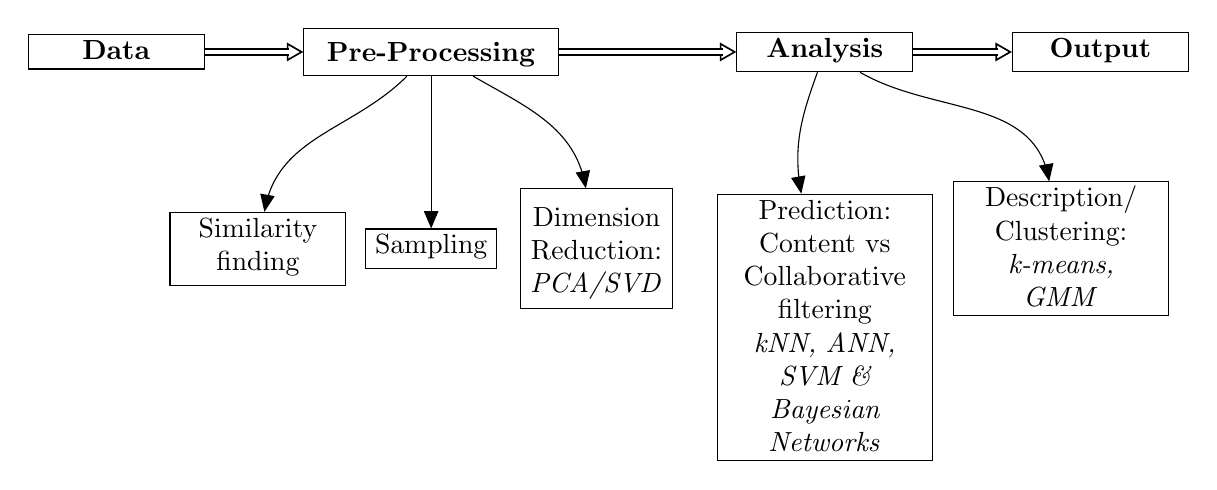
\begin{tikzpicture}
\tikzstyle{vecArrow} = [thick, decoration={markings,mark=at position
   1 with {\arrow[semithick]{open triangle 60}}},
   double distance=1.4pt, shorten >= 5pt,
   preaction = {decorate},
   postaction = {draw,line width=1.4pt, white,shorten >= 4.5pt}]
\node[draw, text width=2cm, text height=0.2cm, align=center] at (1,0) (data){\textbf{Data}};

\node[draw, text width=3cm, text height=0.3cm, align=center] at (5,0) (preproc){\textbf{Pre-Processing}};


\node[draw, text width=2cm, text height=0.2cm, align=center] at (2.8,-2.5) (sim){Similarity finding};
\node[draw, text height=0.2cm, align=center] at (5,-2.5) (sam){Sampling};
\node[draw, text height=1.2cm, align=center] at (7.1,-2.5) (dim){Dimension \\ Reduction:\\ \textit{PCA/SVD}};

\node[draw, text width=2cm, text height=0.2cm, align=center] at (10,0)(analysis) {\textbf{Analysis}};

\node[draw, text width=2.5cm, text height=0.2cm, align=center] at (10,-3.5) (pred){Prediction: \\ Content vs Collaborative filtering \\ \textit{kNN, ANN, SVM \& Bayesian Networks}};
\node[draw, text width=2.5cm, text height=0.2cm, align=center] at (13,-2.5) (desc){Description/\\Clustering: \\ \textit{k-means,} \\ \textit{GMM}};

\node[draw, text width=2cm, text height=0.2cm, align=center] at (13.5,0)(output) {\textbf{Output}};

\draw [vecArrow](data) -- (preproc);
\draw [vecArrow](preproc) -- (analysis);
\draw [vecArrow](analysis) -- (output);
\draw (preproc) edge[in=80,out=-135,->] (sim);
\draw (preproc) edge[->] (sam);
\draw (preproc) edge[out=-30, in=100,->] (dim);

\draw (analysis) edge[out=-110, in=100,->] (pred);
\draw (analysis) edge[out=-30, in=100,->] (desc);
\end{tikzpicture}
\end{figure*}
A typical recommender system works by having multiple data processing stages and active sample selection is part of one of those steps (Figure~\ref*{fig:RecSysDiagram}, explained more in detailed in the Background section, provides a quick overview fo these steps). Thus the first aim is to build a working but flexible recommender system which would include active sample selection. It is expected to base the recommender system on a collaborative filtering model called Probabilistic Matrix Factorization (PMF), which is based on the work of \cite{pmf}. This is because current active sample selection work is often based on this model and this model performs well on large sparse datasets. A library or premade model will not be used as it is less flexible and does not have a useful learning process that will help give insight into the inner workings of a recommender system.

To test the recommender system sample datasets will be used. Several datasets have been identified due to their popularity in recommender systems literature:
\begin{description}[style=standard,leftmargin=.7cm,font=\bfseries]
  \item[MovieLens] is a movie recommendation website that makes subsets of its information(100 thousand, 1 and 10 million ratings in each respective dataset) publicly available for research purposes. Each available dataset is already set-up for use in recommender system testing, with cross-validation and test data already present.
  \item[DrugBank] is a bioinformatics and cheminformatics database that combines detailed drug (i.e., chemical, pharmacological and pharmaceutical) data with comprehensive drug target data. A subset can be downloaded for easier processing and testing. As the data is biological and not user derived it is less likely to contain noise derived from indecisive users and fluctuations of opinions over time.
  \item[Active Learning Challenge] Rather than one dataset, this is a set of datasets used explicitly for an active learning competition, sponsored by two journals \cite{al-chall}. The datasets contained are :
  \begin{itemize}
  \item \underline{HIVA} is a dataset aimed at predicting which compounds are active against the AIDS HIV infection.
  \item \underline{ORANGE} is a noisy marketing dataset. The goal is to predict the likelihood of customers to change network provider, buy complimentary or value-added products or services. 
  \end{itemize}
\end{description}

Small versions (100 thousand entries) of the datasets will be used for development purposes and performance (with respect to error rate and computational intensity) and larger scale use is used for further testing. Synthetic datasets and images will also be used.

Once a working implementation of a recommender system is achieved (this will be done by checking for an acceptable prediction/error rate on the provided test set) focus will be on implementing the work of Sutherland et al.\cite{active-mf}, where his work is made available on his website.

Once this first step is achieved, different methods will be looked at to improve the accuracy or performance of this implementation -  whichever one is determined to be the largest bottleneck. The idea would be to implement either custom ideas or ones present in other papers, such as Jorge Silva's\cite{silva} implementation.

In summary:
\begin{itemize}
\item \textit{Software/language used}: Matlab
\item \textit{Data used}: Synthetic Data, Images, MovieLens, DrugBank and the Active Learning Challenge datasets
\item \textit{Deliverable}: Active sample selection model which should be able to have a better prediction performance than random sampling, ideally with better time complexity.
\end{itemize}

\section{Report Structure}
The report will first give an overview of the various recommender systems (matrix factorisation in particular) with a review of their performance. Given an insight into what matrix factorisation can achieve the concept of active sampling will be introduced by the use of a very basic algorithm. From this a more advanced algorithm is constructed and compared to other already existent algorithms. Performance of each algorithm is compared.
%%% ----------------------------------------------------------------------


%%% Local Variables: 
%%% mode: latex
%%% TeX-master: "../thesis"
%%% End: 

% \pagebreak[4]
% \hspace*{1cm}
% \pagebreak[4]
% \hspace*{1cm}
% \pagebreak[4]
\newcommand\setrow[9]{
  \setcounter{col}{1}
  \foreach \n in {#1, #2, #3, #4, #5, #6, #7, #8, #9} {
    \edef\x{\value{col} - 0.5}
    \edef\y{9.5 - \value{row}}
    \node[anchor=center] at (\x, \y) {\n};
    \stepcounter{col}
  }
  \stepcounter{row}
}
\chapter{Recommender Systems}
\ifpdf
    \graphicspath{{Chapter1/Chapter1Figs/PN1G/}{Chapter1/Chapter1Figs/PDF/}{Chapter1/Chapter1Figs/}}
\else
    \graphicspath{{Chapter1/Chapter1Figs/EPS/}{Chapter1/Chapter1Figs/}}
\fi
\markright{\thechapter. Recommender System Basics}
\section{Basics}
For any decent test of active sample selection a matrix completion algorithm must be used. The basic idea such a system is graphically described in figure \ref{MatrixComp}. We have an incomplete matrix that tells us a certain amount of data about what movies each user likes or dislikes. From this we use a matrix completion algorithm to infer what the empty entries are. This thus allows a system to recommend potential movies a user may like or useful drug-target interactions that have not been tested out.
\begin{figure}[!htbp]
  \begin{center}
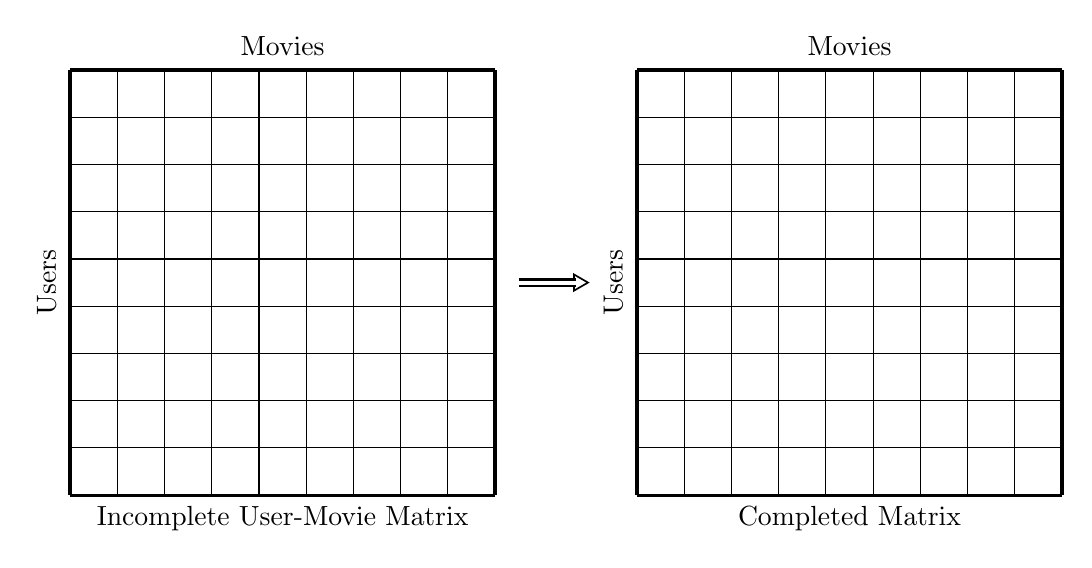
\begin{tikzpicture}[scale=.6]

  \begin{scope}
    \draw (0, 0) grid (9, 9);
    \draw[very thick, scale=9] (0, 0) grid (1, 1);

    \setcounter{row}{1}
    \setrow { }{3}{ }  {5}{ }{5}  { }{ }{ }
    \setrow {1}{ }{ }  { }{ }{ }  { }{4}{ }
    \setrow { }{ }{ }  {4}{3}{ }  {3}{ }{1}

    \setrow { }{3}{ }  { }{4}{ }  {1}{4}{ }
    \setrow { }{ }{2}  {4}{3}{ }  { }{4}{2}
    \setrow { }{ }{ }  { }{3}{ }  { }{ }{1}

    \setrow { }{1}{ }  {2}{ }{2}  { }{ }{ }
    \setrow { }{3}{ }  {4}{ }{ }  {1}{ }{2}
    \setrow { }{ }{ }  {4}{ }{ }  { }{4}{2}

	\node[anchor=center] at (4.5, 9.5) {Movies};
	\node[anchor=center, rotate=90] at (-0.5, 4.5) {Users};
    \node[anchor=center] at (4.5, -0.5) {Incomplete User-Movie Matrix};
  \end{scope}
  
   \begin{scope}
\tikzstyle{vecArrow} = [thick, decoration={markings,mark=at position
   1 with {\arrow[semithick]{open triangle 60}}},
   double distance=1.4pt, shorten >= 5pt,
   preaction = {decorate},
   postaction = {draw,line width=1.4pt, white,shorten >= 4.5pt}]
   
\draw [vecArrow](9.5,4.5) -- (11,4.5);

   \end{scope}

  \begin{scope}[xshift=12cm]
    \draw (0, 0) grid (9, 9);
    \draw[very thick, scale=9] (0, 0) grid (1, 1);

    \setcounter{row}{1}
    \setrow { }{3}{ }  {5}{ }{5}  { }{ }{ }
    \setrow {1}{ }{ }  { }{ }{ }  { }{4}{ }
    \setrow { }{ }{ }  {4}{3}{ }  {3}{ }{1}

    \setrow { }{3}{ }  { }{4}{ }  {1}{4}{ }
    \setrow { }{ }{2}  {4}{3}{ }  { }{4}{2}
    \setrow { }{ }{ }  { }{3}{ }  { }{ }{1}

    \setrow { }{1}{ }  {2}{ }{2}  { }{ }{ }
    \setrow { }{3}{ }  {4}{ }{ }  {1}{ }{2}
    \setrow { }{ }{ }  {4}{ }{ }  { }{4}{2}
    
	\node[anchor=center] at (4.5, 9.5) {Movies};
	\node[anchor=center, rotate=90] at (-0.5, 4.5) {Users};
    \node[anchor=center] at (4.5, -0.5) {Completed Matrix};

    \begin{scope}[blue, font=\sffamily\slshape]
      \setcounter{row}{1}
    \setrow {1}{ }{2}  { }{4}{ }  {2}{4}{2}
    \setrow { }{3}{2}  {4}{3}{4}  {1}{ }{2}
    \setrow {1}{2}{2}  { }{ }{4}  { }{3}{ }

    \setrow {1}{ }{2}  {4}{ }{4}  { }{ }{2}
    \setrow {1}{3}{ }  { }{ }{4}  {1}{ }{ }
    \setrow {1}{2}{1}  {3}{ }{3}  {1}{3}{ }

    \setrow {1}{ }{1}  { }{1}{ }  {1}{2}{1}
    \setrow {1}{ }{2}  { }{4}{4}  { }{4}{ }
    \setrow {1}{3}{2}  { }{3}{4}  {1}{ }{ }
    \end{scope}

  \end{scope}

\end{tikzpicture}
\end{center}
Completed entries have their number represented in blue. Each movie is rated out of 5.
    \caption{Sample Matrix Completion on Movie Data}
    \label{MatrixComp}
  
\end{figure}

Many commercial systems for recommender systems currently exist. For example Amazon, YouTube, Google, Netflix, IMDb and Last.fm are but a small sample of websites using recommender systems to suggest films, ads, music or products to users. In fact Netflix is known for the "Netflix Prize", an open competition that awarded \$1 million to a group of researchers that could create a recommender system achieving a 10\% or more improvement on their previous one.

More formally, a recommender system database comes in matrix form, $R \in \mathbb{R}^{M \times N}$ with each entry containing a numerical quantifier of the relationship between the row item and column item. As not every entry is complete we can associate this to a mask matrix $Z \in \mathbb{R}^{M \times N}$, where $Z_{ij} \in \{0,1\} \forall i,j$. $0$ represents an unknown entry and $1$ a currently known entry.


\nomenclature{RMSE}{Root Mean Square Error -  Measure of differences between values predicted by a model and the actual values:  $\sqrt{\frac{1}{N} \sum\nolimits_{i=1}^{N}(\hat{x}_i-x_i)^2}$}
\nomenclature{CF}{Collaborative Filtering} 
\nomenclature{PMF}{Probabilistic Matrix Factorisation} 
\nomenclature{BPMF}{Bayesian Probabilistic Matrix Factorisation} 



\section{Types of Recommender Systems}


\subsection{Overview}
Recommender systems typically work by having a pre-processing and analysis/matching stage with Figure \ref*{fig:RecSysDiagram} showing the various stages. Pre-processing will typically be clustering the data into groups, reducing the dimensionality (for example by a process similar to SVD) or creating a subset of data that is more manageable. Active sample selection fits in here. Then the actual processing stage is where the empty samples are filled in. There can also be a post-processing stage where certain generated samples are selected either due to their usefulness or high score (i.e. a high predicted product score may be selected as part of a monetisation strategy). 

\nomenclature{SVD}{Singular Value Decomposition - A method to decompose a matrix into smaller dimension matrices}

There are several types of Recommender Systems:
\begin{description}[style=standard,leftmargin=.5cm,font=\bfseries]
\item[Collaborative Filtering] In this type of system the user is placed into sub-groups that have similar taste. From this, it is expected that if user A has similar taste than user B on some products he is more likely to have the same one about different products.
\item[Content-based filtering] In this system features are learned about content (such as item color, film type, music genre etc \ldots) and a user's profile of their tastes is built, allowing products to be recommended by their features rather than group similarity.
\item[Demographic Based] In this system extra data that groups columns or users into categories (based on age or sex for example) is used to recommend users items in their respective category.
\end{description}

Each of the above methods can be done in several different ways and have varying performance. It would thus make sense to select the Netflix prize winner algorithm. However the winning proposal, by a team named "BellKor's Pragmatic Chaos", consisted of an ensemble of various recommender systems. This increases complexity and is not very practical to work with. Thus an algorithm that performs well but simple (and easily built upon) is preferred. This explains the choice of the Probabilistic Matrix Factorisation algorithm. Its RMSE on the Netflix dataset is 0.8861, about 7\% better than Netflix system\footnote{The goal of the Netflix prize was to achieve a performance increase of 10\%}. Bayesian Probabilistic Matrix Factorisation \cite{SalMnih2008}, an extension of PMF, will also quickly be covered due to its good performance on very sparse datasets. Finally it decomposes a matrix into two feature matrices which turn out to be very useful in the goal of active sample selection.

\subsection{Probabilistic Matrix Factorisation}
\label{sec:pmf}
PMF works by assuming that each input sample comes with Gaussian noise. If we decompose $R$ into two matrices $\mathrm{U^{T} V}$ we can describe each item, with index $ij$ as $x_{ij}=\mathbf{u}_{i}^{T}\mathbf{v}_{j}+\epsilon_{ij}$ where $\epsilon_{ij} \sim  \mathcal{N} (0,\sigma^2_\epsilon)$. Equations \ref{eq:rsimeq} and \ref{eq:decomp} provide a quick intuition into the decomposition. The reason we decompose the matrix in two matrices is motivated by the want to extract features from each column and row item. This can be done by performing what is called a latent aspect model, which essentially creates a column and row matrices composed of the features and weightings of these items.
\begin{equation} \label{eq:rsimeq}
R \backsimeq U^{T} \cdot V
\end{equation}
\begin{equation}
 \label{eq:decomp}
U^{T} \cdot V=\begin{bmatrix}
u_{11} & u_{12} & \cdots \\
u_{21} & u_{22}& \cdots \\
u_{31}  & u_{32} & \cdots \\
u_{41}  & u_{42} & \cdots \\
\vdots  & \vdots & \ddots
\end{bmatrix} \cdot \begin{bmatrix}
v_{11} & v_{21} & v_{31} &  \cdots \\[-0.1em] 
v_{12} & v_{22} & v_{32} & \cdots \\[-0.1em]
\vdots & \vdots & \vdots &  \ddots \\[-0.1em]
\end{bmatrix}
\end{equation}

We can choose an arbitrary number of features $D$ to form the matrices $U \in \mathbb{R}^{D\times N}$ and $V \in \mathbb{R}^{D\times M}$. Essentially $U$ and $V$ contain the latent features of each row and column items, with $U_i$ and $V_j$ containing the row and column latent features. Assuming the Gaussian noise we can define the conditional distribution of $R$ as:
\begin{equation}
p(R|U,V,\sigma^2) = \prod_{i=1}^{N} \prod_{j=1}^{M} \left[\mathcal{N}(R_{ij}|U_i^T V_j,\sigma^2)\right]^{Z_{ij}}
\end{equation}
Remember that $Z$ is the mask matrix. $i$ and $j$ are the matrix entry coordinates. In addition to this we place Gaussian priors on row and column feature vectors:
\begin{eqnarray}
p(U|\sigma_U^2) = \prod_{i=1}^{N} \mathcal{N}(U_i|0,\sigma_U^2\mathbf{I}), &   p(V|\sigma_V^2) = \prod_{j=1}^{M} \mathcal{N}(V_j|0,\sigma_V^2\mathbf{I})
\end{eqnarray}
Now we assume row and column independence giving:
\begin{equation*}
P(U,V|\sigma_U^2\mathbf{I},\sigma_V^2\mathbf{I}) = p(U|\sigma_U^2)  p(V|\sigma_V^2)
\end{equation*}
We want to find the likelihood of $U$ and $V$ given the supplied parameters.
\begin{align*}
P(U,V|R,\sigma,\sigma_U^2\mathbf{I},\sigma_V^2\mathbf{I}) &= \dfrac{P(U,V,R|\sigma,\sigma_U^2\mathbf{I},\sigma_V^2\mathbf{I})}{P(R|\sigma^2)} \\
&= \dfrac{P(R|U,V,\sigma^2)P(U,V|\sigma_U^2\mathbf{I},\sigma_V^2\mathbf{I})}{P(R|\sigma^2)} \\
&= \dfrac{P(R|U,V,\sigma^2) p(U|\sigma_U^2)  p(V|\sigma_V^2)}{P(R|\sigma^2)}
\end{align*}
 We take the log likelihood of $P(U,V|R,\sigma,\sigma_U^2\mathbf{I},\sigma_V^2\mathbf{I})$ to maximise it.
\begin{align}
\ln (P(U,V|R,\sigma,\sigma_U^2\mathbf{I},\sigma_V^2\mathbf{I})) &= - \frac{1}{2 \sigma^2} \sum_{i=1}^{N} \sum_{j=1}^{M} Z_{ij}(R_{ij}-U_i^TV_j)^2 - \frac{1}{2\sigma_U^2} \sum_{i=1}^{N} \|U_i\|_{Fro}^2 
\notag \\ &  - \frac{1}{2\sigma_V^2} \sum_{j=1}^{M} \|V_j\|_{Fro}^2 + C \label{eq:pmf_ml_log}
\end{align}
Where C is a number not depending on $U$ or $V$. From this we can get an error function to minimise (by inverting the signs).

\begin{align}
E&=\sum_{i=1}^{N} \sum_{j=1}^{M} Z_{ij}(R_{ij}-U_i^TV_j)^2 + \frac{\lambda_U}{2}\sum_{i=1}^{N} \|U_i\|_{Fro}^2 
+ \frac{\lambda_V}{2} \sum_{j=1}^{M} \|V_j\|_{Fro}^2
\label{eq:pmf_err_func}
\end{align}

With $\lambda_U = \frac{\sigma^2}{\sigma_U^2}$ and $\lambda_V = \frac{\sigma^2}{\sigma_V^2}$ being regularisation parameters. We can remove the mask matrix from the equation and create a cell specific error function:
\begin{align*}
e_{ij}^2= (R_{ij}-U_i^TV_j)^2 + \frac{\lambda_U}{2}\sum_{i=1}^{N} \|U_i\|_{Fro}^2 
+ \frac{\lambda_V}{2} \sum_{j=1}^{M} \|V_j\|_{Fro}^2
\end{align*}

From $e_{ij}^2$ we can find $U$ $V$ satisfying $\underset{U,V}{\argmin} \, E$ through simple gradient descent \cite{nnmf-grad}. We use the simple but effective Widrow-Hoff learning rule:

\begin{align*}
U_{ik}^{t+1} &= U_{ik}^{t} - \mu \frac{\partial}{\partial U_{ik}}(e_{ij}^2) \\
&= U_{ik}^{t} + \mu (2 e_{ij}V_{jk} - \lambda_U  U_{ik}^{t})\\
V_{jk}^{t+1} &= V_{jk}^{t} - \mu \frac{\partial}{\partial V_{jk}}(e_{ij}^2) \\
&= V_{jk}^{t} + \mu (2 e_{ij}U_{ik} - \lambda_V  V_{jk}^{t})\\
\end{align*}
$k$ is the feature index, as defined by $D$, $\mu$ i{\tiny }s the learning rate and $t$ is the iteration index. The steps above are repeated until convergence (as defined by a custom criteria) or a fixed number of iterations. This allows us to learn the features of each column and row. Once $U$ and $V$ are learned we can estimate the full matrix by:
\begin{align}
\hat{R} = U^T V
\end{align}
For very large matrices where only a specific entry is needed a single entry can be predicted by $\hat{R}_{ij} = U_i^T V_j$.
\subsection{Bayesian Probabilistic Matrix Factorisation}
\label{sec:bpmf}
\begin{figure}[!ht]
  \begin{center}
    \begin{tabular}{cc}
      % model_pca.tex
%
% Copyright (C) 2012 Jaakko Luttinen
%
% This file may be distributed and/or modified
%
% 1. under the LaTeX Project Public License and/or
% 2. under the GNU General Public License.
%
% See the files LICENSE_LPPL and LICENSE_GPL for more details.

% PCA model

%\beginpgfgraphicnamed{model-pca}
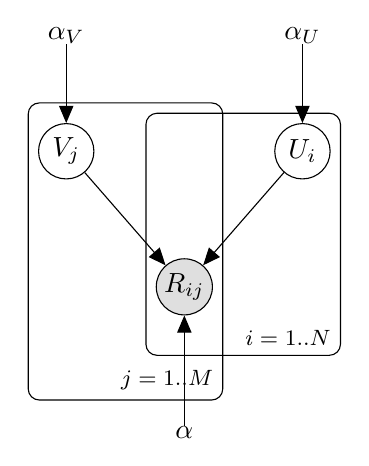
\begin{tikzpicture}

  % Define nodes
  \node[obs]                               (y) {$R_{ij}$};
  \node[latent, above=of y, xshift=-1.5cm] (w) {$V_j$};
  \node[latent, above=of y, xshift=1.5cm]  (x) {$U_i$};
  \node[const, below=1.4cm of y]            (t) {$\alpha$};
  \node[const, above=1cm of w]            (av) {$\alpha_V$};
  \node[const, above=1cm of x]            (au) {$\alpha_U$};

  % Connect the nodes
  \edge {x,w,t} {y} ; %
  \edge {av}{w} ;
  \edge {au}{x} ;

  % Plates
  \plate {yx} {(x)(y)} {$i=1..N$} ;
  \plate {} {(w)(y)(yx.north west)(yx.south west)} {$j=1..M$} ;

\end{tikzpicture}
%\endpgfgraphicnamed

%%% Local Variables: 
%%% mode: tex-pdf
%%% TeX-master: "example"
%%% End: 
 &
      % model_pca.tex
%
% Copyright (C) 2012 Jaakko Luttinen
%
% This file may be distributed and/or modified
%
% 1. under the LaTeX Project Public License and/or
% 2. under the GNU General Public License.
%
% See the files LICENSE_LPPL and LICENSE_GPL for more details.

% PCA model

%\beginpgfgraphicnamed{model-pca}
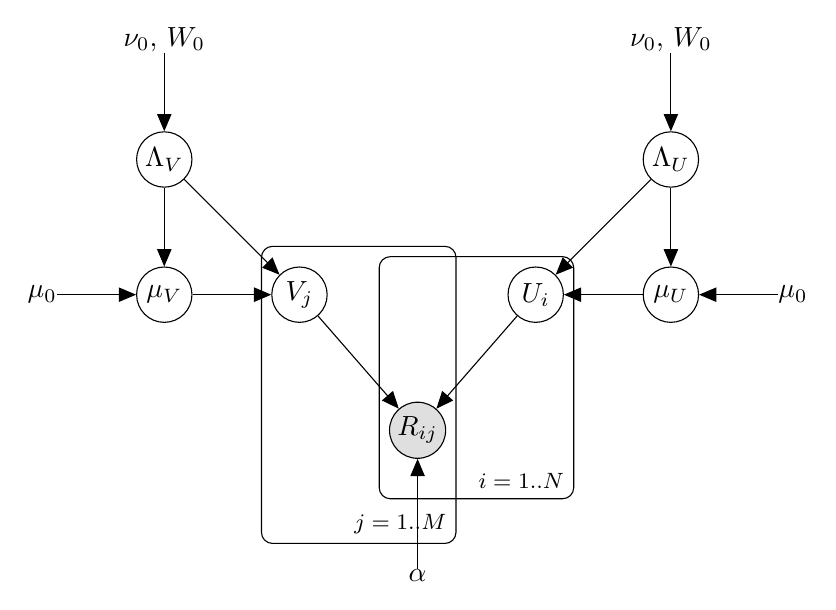
\begin{tikzpicture}

  % Define nodes
  \node[obs]                               (y) {$R_{ij}$};
  \node[latent, above=of y, xshift=-1.5cm] (w) {$V_j$};
  \node[latent, above=of y, xshift=1.5cm]  (x) {$U_i$};
  \node[const, below=1.4cm of y]            (t) {$\alpha$};
  \node[latent, left=1cm of w]            (mv) {$\mu_V$};
  \node[latent, above=1cm of mv]            (lv) {$\Lambda_V$};
  \node[const, left=1cm of mv]            (m0v) {$\mu_0$};
  \node[const, above=1cm of lv]            (l0v) {$\nu_0$, $W_0$};
  
  \node[latent, right=1cm of x]            (mu) {$\mu_U$};
  \node[latent, above=1cm of mu]            (lu) {$\Lambda_U$};
  \node[const, right=1cm of mu]            (m0u) {$\mu_0$};
  \node[const, above=1cm of lu]            (l0u) {$\nu_0$, $W_0$};

  % Connect the nodes
  \edge {x,w,t} {y} ; %
  \edge {mv}{w} ;
  \edge {lv}{mv,w} ;
  \edge {m0v}{mv} ;
  \edge {l0v}{lv} ;
 
  \edge {mu}{x} ;
  \edge {lu}{mu,x} ;
  \edge {m0u}{mu} ;
  \edge {l0u}{lu} ;

  % Plates
  \plate {yx} {(x)(y)} {$i=1..N$} ;
  \plate {} {(w)(y)(yx.north west)(yx.south west)} {$j=1..M$} ;

\end{tikzpicture}
%\endpgfgraphicnamed

%%% Local Variables: 
%%% mode: tex-pdf
%%% TeX-master: "example"
%%% End: 
 \\
      PMF & BPMF
    \end{tabular}
  \end{center}
  \caption{Graphical Model for PMF and BPMF}
  \label{fig:bpmf_pmf_gm}
\end{figure}


Bayesian Probabilistic Matrix Factorisation has been proposed as an extension of PMF \cite{SalMnih2008}. It places Gaussian priors on $U$ and $V$ and Gaussian-Wishart priors on the row and column hyperparameters. A graphical representation to compare to PMF is found in figure \ref{fig:bpmf_pmf_gm}.

\begin{align*}
p(U|\mu_U,\Lambda_U) &= \prod\limits_{i=1}^{N} \mathcal{N}(U_i|\mu_U,\Lambda_U^{-1})\\
p(V|\mu_V,\Lambda_V) &= \prod\limits_{j=1}^{M} \mathcal{N}(V_j|\mu_V,\Lambda_V^{-1})
\end{align*}
$\Lambda^{-1}$ is the precision matrix and $\mu$ is the mean of each feature vector. $\Theta_U=\{\mu_U,\Lambda_U\}$ and $\Theta_V=\{\mu_V,\Lambda_V\}$ are defined as the row and column hyper parameters.
\begin{align*}
p(\Theta_U|\Theta_0) = p(\mu_U|\Lambda_U)p(\Lambda_U)= \mathcal{N}(\mu_U|\mu_0,(\beta_0 \Lambda_U)^{-1})\mathcal{W}(\Lambda_U|W_0, \nu_0) \\
p(\Theta_V|\Theta_0) = p(\mu_V|\Lambda_V)p(\Lambda_V)= \mathcal{N}(\mu_V|\mu_0,(\beta_0 \Lambda_V)^{-1})\mathcal{W}(\Lambda_V|W_0, \nu_0)
\end{align*}
We have $\mathcal{W}$ as the Wishart distribution with $\nu_0$ degrees of freedom and $W_0 \in \mathbb{R}^{D \times D}$. $\Theta_0=\{\mu_0,\nu_0,\Lambda_0\}$ is defined with $\mu_0=0$, $\nu_0=D$ and $W_0=\mathbf{I}_{D\times D}$.
After rearranging we end up with:
\begin{align*}
P(U,V|R,\Theta_U,\Theta_V) =\int \int P(R | U,V) P(U,V | R,\Theta_U,\Theta_V) P(\Theta_U,\Theta_V | \Theta_0)d\Theta_U d\Theta_V
\end{align*}
The above equation cannot be resolved analytically and approximate methods must be used. Thus we resort to a MCMC method, Gibbs sampling. This allows us to generate multiple approximations of $U$ and $V$ feature matrices and then get a better approximation out of it.
\nomenclature{MCMC}{Markov chain Monte Carlo - A means of approximating a probability distribution}
The outline of Gibbs sampling for BPMF is as follows:
\begin{enumerate}
  \item Initialise $U^1$, $V^1$
  \item For $t=1\dots T$
	\begin{itemize}
	  \item Sample hyperparameters $\Theta_U$ and $\Theta_V$
	  \item For $i=1 \dots N$ sample row features in parallel:
	  \begin{align*}
	  U_i^{t+1} \sim p(U_i^t|R, V^t ,\Theta_U^t)
	  \end{align*}
	  \item For $j=1 \dots M$ sample column features in parallel:
	  \begin{align*}
	  V_j^{t+1} \sim p(V_j^t|R, U^t ,\Theta_V^t)
	  \end{align*}
	\end{itemize}
\end{enumerate}
More details on BPMF and can be found in the appendix section \ref{sec:app_bpmf}.

For the purpose of this project it is mainly useful to remember that BPMF performs well on very sparse matrices - in  part due to the MCMC sampling process which provides a good approximation of the true probability distribution of data points.

\subsection{Kernelized Probabilistic Matrix Factorization}
\nomenclature{KMPF}{Kernelized Probabilistic Matrix Factorisation} 
Another variant of PMF that was tested was KMPF \cite{kpmf}. The main ideas to take from it are that it functions like PMF but with the crucial difference that a latent Gaussian process prior is placed over all rows and columns on top of a latent vector on each row and column. This means that it captures side information through kernel matrices that contain the covariance information. The intended use of these kernels is to use separate graph data, such as the social connection between users. However in the case this data does not exist a certain correlation between columns and rows can be assumed, which still results in good performances.

Performance of KPMF is best on very sparse data due to its ability to \textit{smooth} out data from its assumption of inter-row and inter-column correlation. In fact KPMF can work very well on empty rows or columns by filling them in with the most likely values - something PMF and BPMF struggle with.  Once more data on the dataset is available KPMF's performance can even be worse than the traditional model due to forcing these correlations. In the context of active sample selection, where more cells become available over time, this could cause a problem in determining the usefulness of each new discovered cell.
\section{Evaluation and comments}
\subsection{Performance test}

To understand what may be best to use we test each type of algorithm on a dataset. This allows to see its advantages and weaknesses. For the first test we look at figure \ref{fig:5pcmat}.

\begin{figure}[!htbp]
  \begin{center}
    \resizebox{\textwidth}{!}{% This file was created by matlab2tikz v0.4.7 running on MATLAB 8.1.
% Copyright (c) 2008--2014, Nico Schlömer <nico.schloemer@gmail.com>
% All rights reserved.
% Minimal pgfplots version: 1.3
% 
% The latest updates can be retrieved from
%   http://www.mathworks.com/matlabcentral/fileexchange/22022-matlab2tikz
% where you can also make suggestions and rate matlab2tikz.
% 
\begin{tikzpicture}

\begin{axis}[%
width=2.5in,
height=2.5in,
axis on top,
scale only axis,
xmin=0.5,
xmax=50.5,
y dir=reverse,
ymin=0.5,
ymax=80.5,
name=plot2,
title={BPMF $\beta$=1.5 D=10 RMSE=1.4858}
]
\addplot [forget plot] graphics [xmin=0.5,xmax=50.5,ymin=0.5,ymax=80.5] {5pcmatrix-1.png};
\end{axis}

\begin{axis}[%
width=2.5in,
height=2.5in,
axis on top,
scale only axis,
xmin=0.5,
xmax=50.5,
y dir=reverse,
ymin=0.5,
ymax=80.5,
name=plot1,
at=(plot2.left of south west),
anchor=right of south east,
title={PMF $\lambda$=0.1 D=10 RMSE=1.9269}
]
\addplot [forget plot] graphics [xmin=0.5,xmax=50.5,ymin=0.5,ymax=80.5] {5pcmatrix-2.png};
\end{axis}

\begin{axis}[%
width=2.5in,
height=2.5in,
scale only axis,
xmin=0,
xmax=200,
xlabel={Iterations},
xmajorgrids,
ymin=0,
ymax=3,
ylabel={Training RMSE},
ymajorgrids,
name=plot4,
at=(plot1.below south west),
anchor=above north west,
title={PMF learning rate}
]
\addplot [color=blue,solid,forget plot]
  table[row sep=crcr]{1	2.9957906513364\\
2	2.99573240721177\\
3	2.99567087079752\\
4	2.99560398509265\\
5	2.99552944277968\\
6	2.99544457608174\\
7	2.99534622706284\\
8	2.99523059115264\\
9	2.99509302512218\\
10	2.99492780867601\\
11	2.99472784614834\\
12	2.99448429136208\\
13	2.99418607436785\\
14	2.99381930334373\\
15	2.99336650821599\\
16	2.99280568438519\\
17	2.99210908521507\\
18	2.99124170073898\\
19	2.99015934778069\\
20	2.98880628441992\\
21	2.98711225159157\\
22	2.98498884051027\\
23	2.98232509328052\\
24	2.97898227636352\\
25	2.97478783909222\\
26	2.96952870557859\\
27	2.9629442777942\\
28	2.95471988090916\\
29	2.94448187572308\\
30	2.93179626868344\\
31	2.91617324245813\\
32	2.89708032539367\\
33	2.87396644545731\\
34	2.84629732187906\\
35	2.81359927710866\\
36	2.77550428936809\\
37	2.73178610650202\\
38	2.68237855815169\\
39	2.62737436043846\\
40	2.56701265929176\\
41	2.50166889237266\\
42	2.43185545900871\\
43	2.35822904747324\\
44	2.2815908321882\\
45	2.20286717493098\\
46	2.12306850148217\\
47	2.04323341127009\\
48	1.96436780813024\\
49	1.88738658206482\\
50	1.813063007095\\
51	1.74199062760765\\
52	1.67456234235614\\
53	1.61096952933276\\
54	1.55122034782063\\
55	1.49517255046433\\
56	1.44257397351365\\
57	1.39310389892452\\
58	1.34641012611975\\
59	1.30213885061277\\
60	1.25995649081079\\
61	1.21956401494873\\
62	1.18070504334836\\
63	1.14316918830491\\
64	1.10679195620598\\
65	1.07145225951035\\
66	1.03706829752675\\
67	1.00359233383394\\
68	0.971004748523338\\
69	0.939307669076093\\
70	0.908518462325837\\
71	0.878663374149575\\
72	0.84977160838898\\
73	0.82187012422418\\
74	0.794979392714515\\
75	0.76911028767131\\
76	0.744262199288707\\
77	0.720422361470927\\
78	0.69756628832028\\
79	0.675659134456531\\
80	0.654657737871361\\
81	0.634513078513625\\
82	0.615172890885836\\
83	0.596584199641218\\
84	0.578695595085115\\
85	0.561459121046717\\
86	0.544831702289787\\
87	0.528776086465032\\
88	0.513261313526749\\
89	0.498262753077555\\
90	0.483761768507088\\
91	0.469745078018227\\
92	0.456203888584848\\
93	0.443132880925406\\
94	0.430529122417648\\
95	0.418390980711125\\
96	0.406717103562855\\
97	0.39550552013768\\
98	0.384752905992009\\
99	0.374454038929302\\
100	0.36460145699923\\
101	0.355185314470331\\
102	0.346193418011223\\
103	0.337611414716886\\
104	0.329423096750327\\
105	0.321610784462664\\
106	0.314155750631027\\
107	0.307038652236959\\
108	0.300239942077499\\
109	0.29374023946558\\
110	0.287520646425914\\
111	0.281563002403608\\
112	0.275850076089079\\
113	0.27036569727607\\
114	0.265094834664483\\
115	0.260023627300645\\
116	0.255139378109963\\
117	0.250430517955989\\
118	0.245886548091405\\
119	0.241497967960482\\
120	0.237256194240643\\
121	0.233153475901463\\
122	0.229182809001198\\
123	0.225337853988034\\
124	0.221612857453017\\
125	0.218002579602373\\
126	0.214502228173589\\
127	0.211107399099781\\
128	0.207814023914021\\
129	0.204618323661903\\
130	0.201516768939631\\
131	0.198506045580991\\
132	0.195583025466306\\
133	0.192744741908713\\
134	0.189988369078752\\
135	0.18731120495017\\
136	0.184710657282246\\
137	0.182184232192865\\
138	0.179729524918503\\
139	0.177344212400268\\
140	0.175026047377274\\
141	0.172772853708979\\
142	0.170582522685899\\
143	0.168453010122892\\
144	0.166382334060845\\
145	0.164368572930905\\
146	0.162409864060639\\
147	0.160504402423542\\
148	0.158650439552621\\
149	0.156846282555277\\
150	0.155090293180899\\
151	0.153380886904451\\
152	0.151716531999314\\
153	0.150095748580831\\
154	0.148517107608674\\
155	0.146979229841494\\
156	0.145480784741487\\
157	0.144020489329753\\
158	0.142597106995693\\
159	0.14120944626541\\
160	0.13985635953521\\
161	0.138536741777016\\
162	0.137249529222785\\
163	0.135993698035103\\
164	0.134768262970903\\
165	0.133572276044958\\
166	0.132404825199296\\
167	0.131265032984191\\
168	0.130152055255781\\
169	0.129065079894787\\
170	0.128003325550198\\
171	0.126966040411223\\
172	0.12595250101023\\
173	0.12496201105892\\
174	0.123993900319442\\
175	0.123047523511773\\
176	0.122122259258242\\
177	0.121217509065769\\
178	0.120332696346031\\
179	0.119467265473537\\
180	0.118620680881329\\
181	0.117792426193838\\
182	0.116982003396267\\
183	0.116188932039702\\
184	0.115412748481079\\
185	0.11465300515702\\
186	0.113909269890489\\
187	0.113181125229173\\
188	0.112468167814452\\
189	0.111770007779813\\
190	0.11108626817754\\
191	0.110416584432518\\
192	0.109760603822016\\
193	0.109117984980294\\
194	0.108488397426935\\
195	0.107871521117811\\
196	0.107267046017633\\
197	0.10667467169305\\
198	0.106094106925321\\
199	0.105525069341596\\
200	0.104967285063899\\
};
\end{axis}

\begin{axis}[%
width=2.5in,
height=2.5in,
axis on top,
scale only axis,
xmin=0.5,
xmax=50.5,
y dir=reverse,
ymin=0.5,
ymax=80.5,
name=plot5,
at=(plot4.right of south east),
anchor=left of south west,
title={Original Data}
]
\addplot [forget plot] graphics [xmin=0.5,xmax=50.5,ymin=0.5,ymax=80.5] {5pcmatrix-3.png};
\end{axis}

\begin{axis}[%
width=2.5in,
height=2.5in,
axis on top,
scale only axis,
xmin=0.5,
xmax=50.5,
y dir=reverse,
ymin=0.5,
ymax=80.5,
name=plot6,
at=(plot5.right of south east),
anchor=left of south west,
title={Data available to algorithms 5\%}
]
\addplot [forget plot] graphics [xmin=0.5,xmax=50.5,ymin=0.5,ymax=80.5] {5pcmatrix-4.png};
\end{axis}

\begin{axis}[%
width=2.5in,
height=2.5in,
axis on top,
scale only axis,
xmin=0.5,
xmax=50.5,
y dir=reverse,
ymin=0.5,
ymax=80.5,
at=(plot6.above north west),
anchor=below south west,
title={KPMF $\sigma$=8 D=10 RMSE=1.3254}
]
\addplot [forget plot] graphics [xmin=0.5,xmax=50.5,ymin=0.5,ymax=80.5] {5pcmatrix-5.png};
\end{axis}
\end{tikzpicture}%}
    Each colour is made to represent a rating out of 5. Dark blue represents a 1 and red a rating of 5. The mean is represented in green.
    
    A row could be used to represent a user and a column a movie.
    \caption{Rating Predictions on synthetic data 5\% complete}
     \label{fig:5pcmat}
  \end{center}
\end{figure}
\begin{figure}[!htbp]
  \begin{center} 
    \resizebox{\textwidth}{!}{% This file was created by matlab2tikz v0.4.7 running on MATLAB 8.1.
% Copyright (c) 2008--2014, Nico Schlömer <nico.schloemer@gmail.com>
% All rights reserved.
% Minimal pgfplots version: 1.3
% 
% The latest updates can be retrieved from
%   http://www.mathworks.com/matlabcentral/fileexchange/22022-matlab2tikz
% where you can also make suggestions and rate matlab2tikz.
% 
\begin{tikzpicture}

\begin{axis}[%
width=2.5in,
height=2.5in,
axis on top,
scale only axis,
xmin=0.5,
xmax=50.5,
y dir=reverse,
ymin=0.5,
ymax=80.5,
name=plot2,
title={BPMF $\beta$=4 D=7 RMSE=1.0815}
]
\addplot [forget plot] graphics [xmin=0.5,xmax=50.5,ymin=0.5,ymax=80.5] {15pcmatrix-1.png};
\end{axis}

\begin{axis}[%
width=2.5in,
height=2.5in,
axis on top,
scale only axis,
xmin=0.5,
xmax=50.5,
y dir=reverse,
ymin=0.5,
ymax=80.5,
at=(plot2.left of south west),
anchor=right of south east,
title={PMF $\lambda$=0.01 D=7 RMSE=1.1015}
]
\addplot [forget plot] graphics [xmin=0.5,xmax=50.5,ymin=0.5,ymax=80.5] {15pcmatrix-2.png};
\end{axis}

\begin{axis}[%
width=2.5in,
height=2.5in,
axis on top,
scale only axis,
xmin=0.5,
xmax=50.5,
y dir=reverse,
ymin=0.5,
ymax=80.5,
at=(plot2.right of south east),
anchor=left of south west,
title={Data available to algorithms 15\%}
]
\addplot [forget plot] graphics [xmin=0.5,xmax=50.5,ymin=0.5,ymax=80.5] {15pcmatrix-3.png};
\end{axis}
\end{tikzpicture}%}
    For KPMF: RMSE=1.1867 for $\sigma=10$
    \caption{Rating Predictions on synthetic data 15\% complete}
    \label{fig:15pcmat}
  \end{center}
\end{figure}
For this figure data was randomly generate by generating 2 matrices $U \in \mathbb{R}^{80\times 5}$ and $V \in \mathbb{R}^{50\times 5}$, that is 5 latent features. A  random mask allowing the variants of PMF to only access 5\% of the data was made and used for matrix completion. The Root Mean Square Error(RMSE) of the predicted data was used as a measure of success. According to RMSE the best performing algorithm is KPMF, which was on average 1.3 off the real value. However all it has effectively done is predicted the mean with some amount of variation for all unknown values. We can see the effect of Gibbs sampling from BPMF as it captures the data distribution better than PMF or KPMF. Despite this it has a higher RMSE. This is one weakness of RMSE as some data sets may penalise more for guessing a value off the mean than one nearer to the mean. Finally PMF is seen to perform the worse, simply failing to predict many entries having very little information.

Making more data available, such as 15 \% of the dataset lead to an improvement for both BPMF and PMF as seen in figure \ref{fig:15pcmat}. PMF experienced the largest RMSE decrease -  something to keep in mind for sample selection. KPMF's RMSE has also improved however its output did not look any better.
\begin{figure}[!htbp]
  \begin{center}
    \resizebox{\textwidth}{!}{% This file was created by matlab2tikz v0.4.7 running on MATLAB 8.1.
% Copyright (c) 2008--2014, Nico Schlömer <nico.schloemer@gmail.com>
% All rights reserved.
% Minimal pgfplots version: 1.3
% 
% The latest updates can be retrieved from
%   http://www.mathworks.com/matlabcentral/fileexchange/22022-matlab2tikz
% where you can also make suggestions and rate matlab2tikz.
% 
\begin{tikzpicture}

\begin{axis}[%
width=2.5in,
height=2.5in,
axis on top,
scale only axis,
xmin=0.5,
xmax=300.5,
y dir=reverse,
ymin=0.5,
ymax=300.5,
name=plot2,
title={BPMF $\beta$=3.5 D=120 RMSE=0.4224}
]
\addplot [forget plot] graphics [xmin=0.5,xmax=300.5,ymin=0.5,ymax=300.5] {eiffel_tower-1.png};
\end{axis}

\begin{axis}[%
width=2.5in,
height=2.5in,
axis on top,
scale only axis,
xmin=0.5,
xmax=300.5,
y dir=reverse,
ymin=0.5,
ymax=300.5,
name=plot1,
at=(plot2.left of south west),
anchor=right of south east,
title={PMF $\lambda$=0.01 D=120 RMSE=0.36275}
]
\addplot [forget plot] graphics [xmin=0.5,xmax=300.5,ymin=0.5,ymax=300.5] {eiffel_tower-2.png};
\end{axis}

\begin{axis}[%
width=2.5in,
height=2.5in,
axis on top,
scale only axis,
xmin=0.5,
xmax=300.5,
y dir=reverse,
ymin=0.5,
ymax=300.5,
name=plot4,
at=(plot1.below south west),
anchor=above north west,
title={PMF $\lambda$=0.05 D=150 RMSE=0.3666}
]
\addplot [forget plot] graphics [xmin=0.5,xmax=300.5,ymin=0.5,ymax=300.5] {eiffel_tower-3.png};
\end{axis}

\begin{axis}[%
width=2.5in,
height=2.5in,
axis on top,
scale only axis,
xmin=0.5,
xmax=300.5,
y dir=reverse,
ymin=0.5,
ymax=300.5,
name=plot5,
at=(plot4.right of south east),
anchor=left of south west,
title={Original Image}
]
\addplot [forget plot] graphics [xmin=0.5,xmax=300.5,ymin=0.5,ymax=300.5] {eiffel_tower-4.png};
\end{axis}

\begin{axis}[%
width=2.5in,
height=2.5in,
axis on top,
scale only axis,
xmin=0.5,
xmax=300.5,
y dir=reverse,
ymin=0.5,
ymax=300.5,
name=plot6,
at=(plot5.right of south east),
anchor=left of south west,
title={Data available to algorithms 88.23\%}
]
\addplot [forget plot] graphics [xmin=0.5,xmax=300.5,ymin=0.5,ymax=300.5] {eiffel_tower-5.png};
\end{axis}

\begin{axis}[%
width=2.5in,
height=2.5in,
axis on top,
scale only axis,
xmin=0.5,
xmax=300.5,
y dir=reverse,
ymin=0.5,
ymax=300.5,
at=(plot6.above north west),
anchor=below south west,
title={KPMF $\sigma$=10 D=120 RMSE=0.6856}
]
\addplot [forget plot] graphics [xmin=0.5,xmax=300.5,ymin=0.5,ymax=300.5] {eiffel_tower-6.png};
\end{axis}
\end{tikzpicture}%}
    Image corrupted by drawing over and virtual spray paint
    \caption{Image Restoration}
    \label{fig:eiffel_tower}
  \end{center}
\end{figure}

In an effort to better understand each algorithm an image restoration trial was done. This is possible due to the rows and columns (pixel wise) in images to exhibit features about them. For example a column may have features indicating 45\% sky hue, 25\% Eiffel tower hue and 30\% ground hue with a row another having its own distribution. Multiplying both together would give the best estimate of the pixel at the specific row-column combination.
In figure \ref{fig:eiffel_tower} a picture with drawing over was supplied to each PMF variant. This was equivalent with supplying 88\% of the data. This time the scales are reversed, with PMF coming out as the clear winner. Not only is the image very similar to the original but little corruption in the overall restoration happened. BPMF failed at this task and distorted the picture overall, blurring it up\footnote{In a practical application of this algorithm it would be possible to only replace the unknown pixels.}. KPMF was able to restore the know pixels correctly but did not do a good job of predicting the missing ones, choosing to predict the mean color instead. KMPF is supposed to provide superior image restoration if supplied the correct kernel \cite{kpmf}. However, despite providing a diffusion kernel indicating that each pixel is correlated to its neighbouring ones, KPMF did not live up to the task.


For the purpose of this project mainly PMF and BPMF will be used as they showed the most promising performances and can be easily customised and built upon. This is especially useful as active sampling builds on top of recommender systems.

Note that the used datasets, synthetic and movielens, have their values ranging from 1 to 5. Thus a RMSE of 2 would mean that predictions are off by 2 stars on average. A good RMSE would thus be under 1, meaning movie predictions are only off by 1 star or less. When possible, other datasets used will be normalised between 1 and 5 to have the RMSE somewhat comparable.

\subsection{Choosing parameters}
All the above PMF variants all relied on one or many parameters. For example PMF uses\footnote{This is actually a combination of $\lambda_U$ and $\lambda_V$ from equation \ref{eq:pmf_err_func}} $\lambda$. These parameters nearly always affect the system performance and choosing them correctly is essential. While it is possible optimise them as such:
\begin{align*}
\underset{U,V,\lambda}{\argmin}\, E(U,V,\lambda)
\end{align*}
This is not a good idea. Indeed $\lambda$ is a regularisation parameter needed to allow the function to correctly generalise\footnote{In an optimisation context it can be seen as a Lagrange multiplier that enforces a constraint} and if optimised in a similar way it would tend to 0 defeating its purpose, see \ref{sec:lag_lambd_optim}. It would essentially perfectly (over)fit the data but not perform predictions correctly. 

Other parameters, such as D (the number of features), could be optimised in a similar way but this increases complexity necessarily. Instead these parameters are usually tweaked by hand and this is what has been done here as this is not the main focus of research.
\subsubsection{Learning rate $\mu$}

$\mu$ is an essential parameter to most iterative learning algorithms. It is appropriately called the learning rate as it defines the rate at which parameters are learnt. If we imagine a convex curve and we are located at a random location on it $\mu$ essentially defines how far we can go on each iteration to get closer to the minimum. Should it be too small a very high number of iterations will be needed to reach satisfactory performance. A too large learning rate may fail to converge due to the steps "jumping around" a minimum but never reaching it - alternatively it could simply overflow with the error increasing at each iteration.

\subsection{Pre-Processing datasets}
Before processing data, it is often advisable to pre-process it. This means cleaning up the data in ways that ensure good performance.
\subsubsection{Normalisation}
The first step that is often taken is to normalise data between two values - by convention 0 and 1 \footnote{For other types of learning algorithms normalisation may be between $[-1,1]$ and zero meaned.}. This ensures that some parameters used, such as regularisation or precision, need not be tweaked a lot when switching between datasets. Additionally when performing gradient descent (as in section \ref{sec:pmf}) over multiple dimensions it is preferable the error for each datapoint is in a similar order of magnitude.
\subsubsection{Discrete Data}
Discrete data is data that only takes a fixed number of values, which is applicable to movie-user datasets where a 5 star rating is given. To process these data is first be normalised between 0 and 1, 0 representing 1 and 1 representing 5. From this, parameters are learnt and data can be predicted. Placing the values back between 1 and 5 will result in non-integer values. Expectedly values are rounded up or down accordingly. Since $3.1$ and $3.45$ will both be rounded down to $3$ we can use the decimal as a measure of uncertainty, that is $3.1$ has a greater probability of actually being $3$ rather than $3.45$. While this is not a fail safe system the deviation from the discrete values can be useful for measuring uncertainty in the model.
\subsection{Online vs Offline learning}
Usually data will be fed to an algorithm and parameters returned to be used for prediction. However there are instances when new data points will be made available and a better performance will be achieved by retraining the parameters with the new data. When a model is retrained from scratch it is said to be done offline. Doing it online means training it once initially and then only carrying out a few steps to update the model when a new sample is received. Collaborative Filtering Algorithms, such as PMF, can be made online \cite{onlinepmf} by first training $U$ and $V$ for initial data and then updating these parameters at each incoming sample.

\begin{table}[!htb]
 \begin{tabular}{l|p{0.4\textwidth}|p{0.4\textwidth}|}
  & \textbf{Online} & \textbf{Offline} \\ \hline
  \textbf{Pro} & Fast update, less iterations  &  Adapts better to new items \\
 & Reuses parameters  & Less local minima issues   \\  \hline
    \textbf{Con} &   Can get stuck in local minima  &     Time intensive    \\
    & & Reinitialises parameters \\
    \hline
 \end{tabular}
 \caption{Comparison of online and offline matrix completion algorithms}
 \label{table:online_offline}
\end{table}


Table \ref{table:online_offline} shows a comparison of the pros and cons of online and offline learning for matrix factorisation systems. The general problem with online PMF is that the error function for PMF \ref{eq:pmf_err_func} is biconvex in $U$ and $V$ and that the minimum is found by alternatively updating each variable, which does not ensure global minimum. Thus if the parameters are stuck in a local minimum online updating will not help and randomly reinitialising them will be better. This is why we will default to using offline updating for the purpose of this report.


\subsection{Test and Validation dataset}
\begin{figure}[!htbp]
  \begin{center} 
    \resizebox{\textwidth}{!}{% This file was created by matlab2tikz v0.4.7 running on MATLAB 8.1.
% Copyright (c) 2008--2014, Nico Schlömer <nico.schloemer@gmail.com>
% All rights reserved.
% Minimal pgfplots version: 1.3
% 
% The latest updates can be retrieved from
%   http://www.mathworks.com/matlabcentral/fileexchange/22022-matlab2tikz
% where you can also make suggestions and rate matlab2tikz.
% 
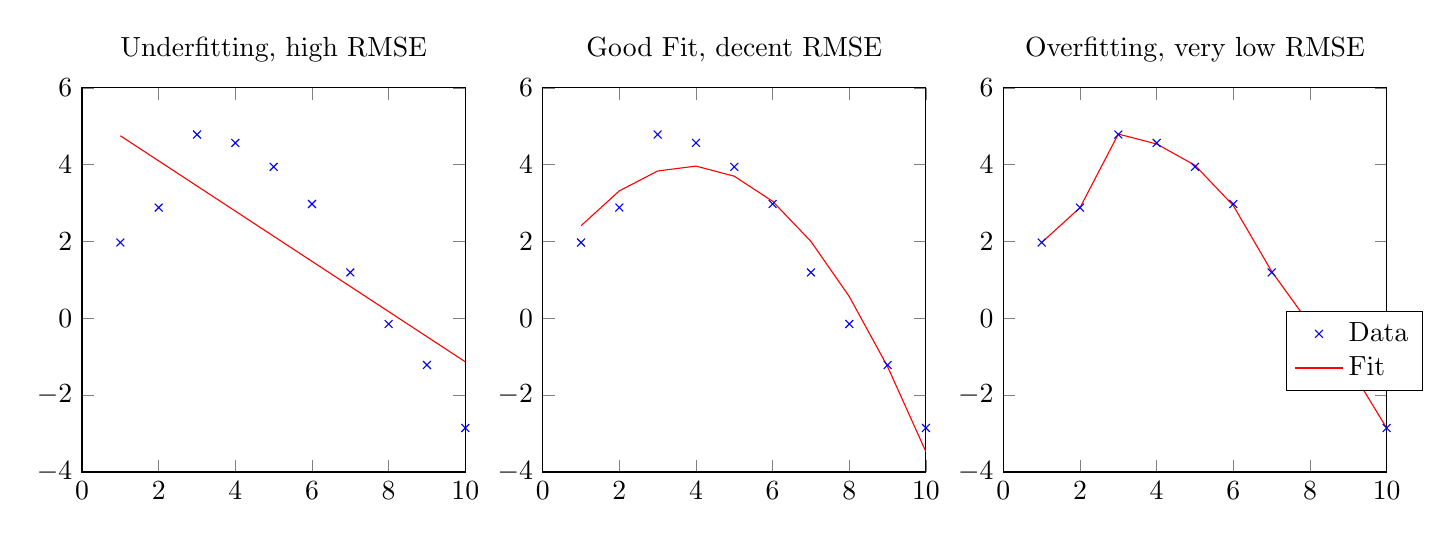
\begin{tikzpicture}

\begin{axis}[%
width=1.91620621980676in,
height=1.92052083333333in,
scale only axis,
xmin=0,
xmax=10,
ymin=-4,
ymax=6,
name=plot2,
title={Good Fit, decent RMSE}
]
\addplot [color=blue,only marks,mark=x,mark options={solid},forget plot]
  table[row sep=crcr]{1	1.97374569656748\\
2	2.88406786873516\\
3	4.78553661488987\\
4	4.5675745314657\\
5	3.94342674696089\\
6	2.9770548882854\\
7	1.19483170610871\\
8	-0.14695915605463\\
9	-1.21420046517419\\
10	-2.85419171271952\\
};
\addplot [color=red,solid,forget plot]
  table[row sep=crcr]{1	2.41023287753905\\
2	3.31851727633452\\
3	3.83626634177898\\
4	3.96348007387242\\
5	3.70015847261484\\
6	3.04630153800625\\
7	2.00190927004665\\
8	0.566981668736026\\
9	-1.25848126592561\\
10	-3.47447953393826\\
};
\end{axis}

\begin{axis}[%
width=1.91620621980676in,
height=1.92052083333333in,
scale only axis,
xmin=0,
xmax=10,
ymin=-4,
ymax=6,
at=(plot2.left of south west),
anchor=right of south east,
title={Underfitting, high RMSE}
]
\addplot [color=blue,only marks,mark=x,mark options={solid},forget plot]
  table[row sep=crcr]{1	1.97374569656748\\
2	2.88406786873516\\
3	4.78553661488987\\
4	4.5675745314657\\
5	3.94342674696089\\
6	2.9770548882854\\
7	1.19483170610871\\
8	-0.14695915605463\\
9	-1.21420046517419\\
10	-2.85419171271952\\
};
\addplot [color=red,solid,forget plot]
  table[row sep=crcr]{1	4.75344487764515\\
2	4.09958794303656\\
3	3.44573100842797\\
4	2.79187407381938\\
5	2.13801713921079\\
6	1.48416020460219\\
7	0.830303269993603\\
8	0.176446335385012\\
9	-0.47741059922358\\
10	-1.13126753383217\\
};
\end{axis}

\begin{axis}[%
width=1.91620621980676in,
height=1.92052083333333in,
scale only axis,
xmin=0,
xmax=10,
ymin=-4,
ymax=6,
at=(plot2.right of south east),
anchor=left of south west,
title={Overfitting, very low RMSE},
legend style={at={(0.737312217300616,0.210441045204993)},anchor=south west,draw=black,fill=white,legend cell align=left}
]
\addplot [color=blue,only marks,mark=x,mark options={solid}]
  table[row sep=crcr]{1	1.97374569656748\\
2	2.88406786873516\\
3	4.78553661488987\\
4	4.5675745314657\\
5	3.94342674696089\\
6	2.9770548882854\\
7	1.19483170610871\\
8	-0.14695915605463\\
9	-1.21420046517419\\
10	-2.85419171271952\\
};
\addlegendentry{Data};

\addplot [color=red,solid]
  table[row sep=crcr]{1	1.97407548210884\\
2	2.88109979888774\\
3	4.79740889434664\\
4	4.53987254606422\\
5	3.98497972506559\\
6	2.93550191018698\\
7	1.22253369151728\\
8	-0.158831435498733\\
9	-1.21123239530863\\
10	-2.85452149827793\\
};
\addlegendentry{Fit};

\end{axis}
\end{tikzpicture}%}
    \caption{Examples of different model fitting}
    \label{fig:over_underfit}
  \end{center}
\end{figure}
From section \ref{sec:pmf} we see that learning from a dataset involves minimising an error function. The problem with this is that we are subject to a "tunnel vision" where only the given data is considered while minimising the error function. A model that only fits the test data, as in figure \ref{fig:over_underfit}, can overfit it and not generalise well. This is one of the reason the regularisation parameters $\lambda_U$ and $\lambda_V$ exist, as they avoid $U$ and $V$ becoming too large and only being specific to the test data. Another way to avoid this is to consider splitting up the dataset into a test set and a validation set. The test set will be used for training. However at each parameter step update, we can calculate the RMSE from the validation data - i.e. data not used for training. As soon as a step is found to lead to an increase of validation RMSE we can infer that the model is potentially starting to overfit and stopping training of parameters is preferable.

\subsection{Data quality}
Another issue with any machine learning system is that of data quality. Any inaccurate or badly generated data can prove to be a major bottleneck in the performance of machine learning systems. Many datasets, especially when they come from human made sources (such as film ratings or opinion polls), have a lot of noise. Noise is essentially the $\epsilon_{ij}$ component which we referred to earlier and creating a model assuming a certain amount of noise is one of the first steps that can be taken to deal with this issue. Note that only incidental noise rather than intentional noise can be dealt with (intentional noise would be defined as data that is maliciously entered or be subject to a strong bias for external reasons). Incidental noise could be reduced to a certain extent by grouping items or users into categories and smoothing out the similar ratings. This and similar techniques can introduce bias in the system and their use is only suggested if it translates to real-world performance increase. Other methods to reduce noise include re-querying a particular sample (\cite{toledo13} i.e. asking a user to re-rate an item, or performing the same experiment again), however this will not be done as the aim of this project is to reduce requeries as well as the fact that we cannot just ask for a data-point to be re-evaluated in our datasets.

To avoid these issues most simulations will be carried on synthetic data, which is less affected by noise.


%... and some more ...
%
%Now I would like to cite the following: \cite{latex} and \cite{texbook}
%and \cite{Rud73}.
%
%I would also like to include a picture ...
%
%\begin{figure}[!htbp]
%  \begin{center}
%    \leavevmode
%    \ifpdf
%      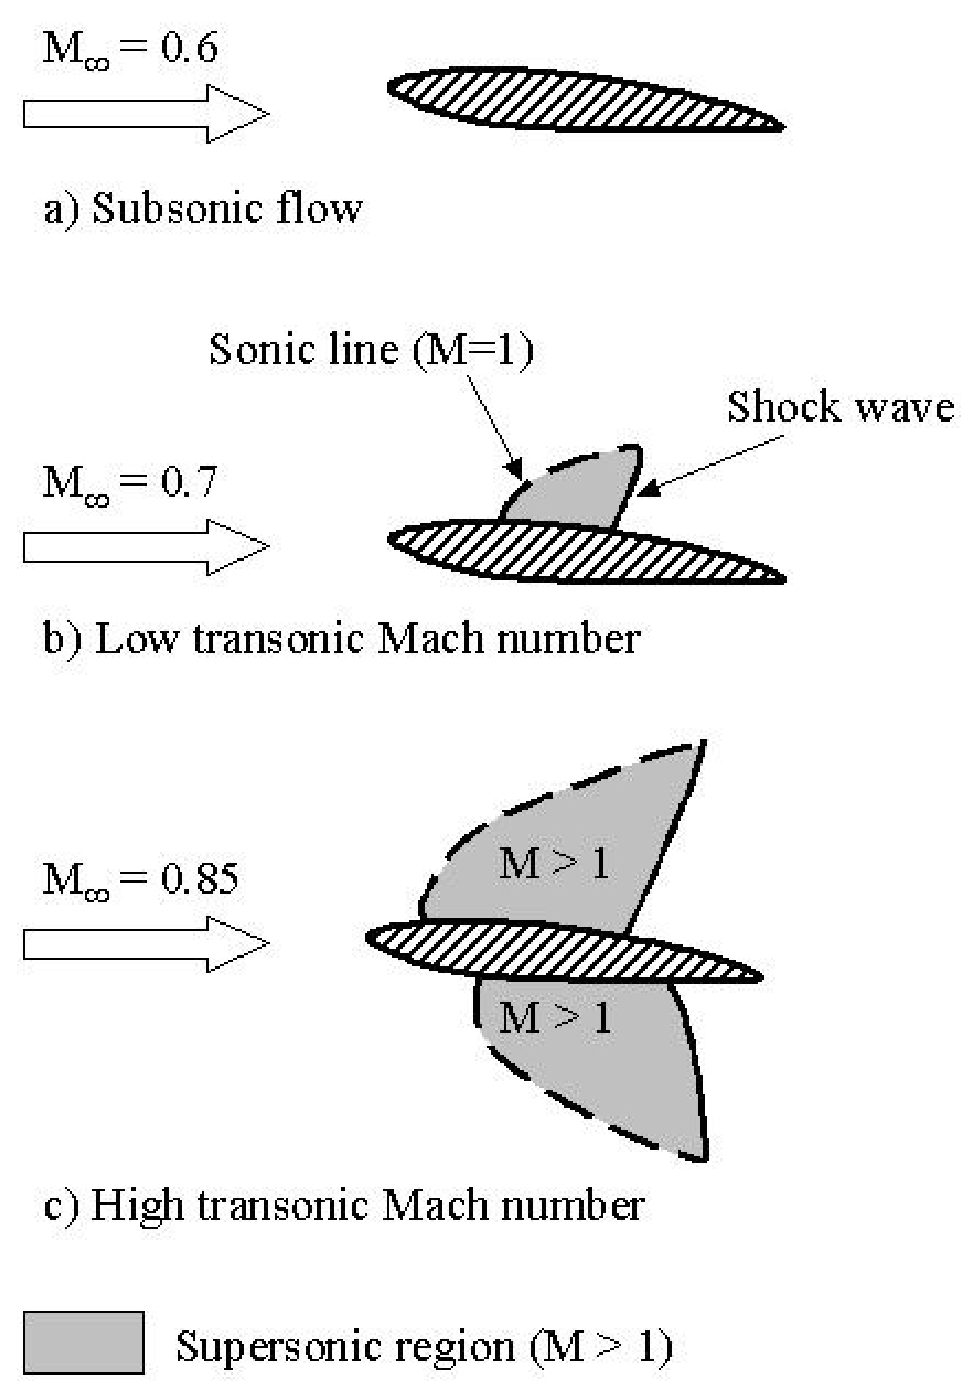
\includegraphics[height=6in]{aflow}
%    \else
%      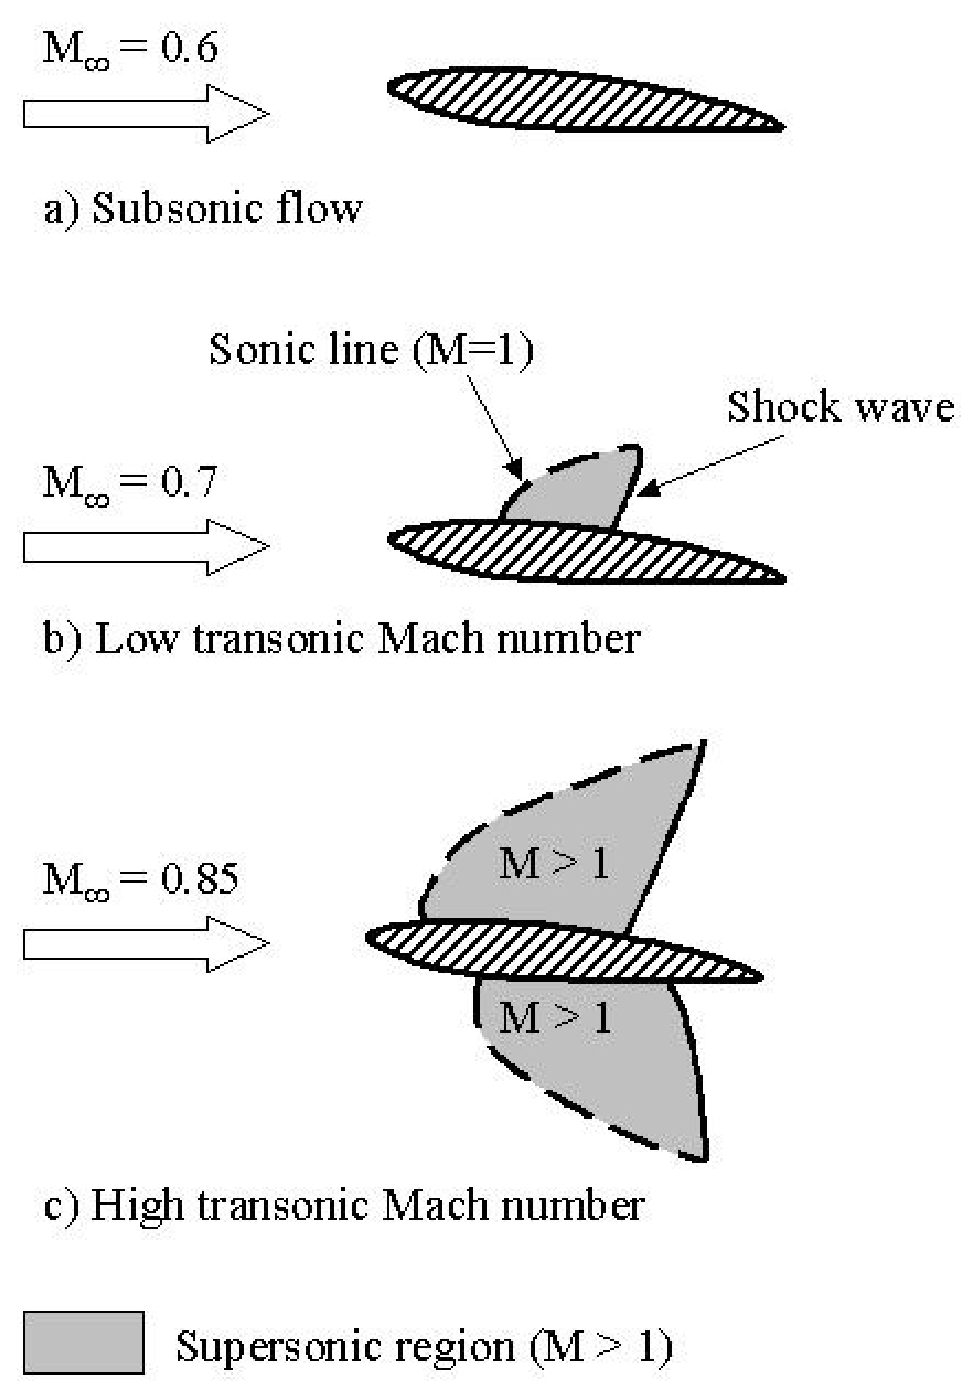
\includegraphics[bb = 92 86 545 742, height=6in]{aflow}
%    \fi
%    \caption{Airfoil Picture}
%    \label{FigAir}
%  \end{center}
%\end{figure}
%
%% above code has been macro-fied in Classes/MacroFile.tex file
%%\InsertFig{\IncludeGraphicsH{aflow}{6in}{92 86 545 742}}{Airfoil Picture}{FigAir}
%
%So as we have now labelled it we can reference it, like so (\ref{FigAir}) and it
%is on Page \pageref{FigAir}. And as we can see, it is a very nice picture and we
%can talk about it all we want and when we are tired we can move on to the next
%chapter ...
%
%I would also like to add an extra bookmark in acroread like so ...
%\ifpdf
%  \pdfbookmark[2]{bookmark text is here}{And this is what I want bookmarked}
%\fi
% ------------------------------------------------------------------------


%%% Local Variables: 
%%% mode: latex
%%% TeX-master: "../thesis"
%%% End: 

\chapter{Active Sample Selection}
\ifpdf
    \graphicspath{{Chapter2/Chapter2Figs/PNG/}{Chapter2/Chapter2Figs/PDF/}{Chapter2/Chapter2Figs/}}
\else
    \graphicspath{{Chapter2/Chapter2Figs/EPS/}{Chapter2/Chapter2Figs/}}
\fi
\markright{\thechapter. Active Sample Selection}
\section{Background}

%\markboth{\MakeUppercase{\thechapter. My Second Chapter }}
Now that we have a good understanding of what matrix factorisation can do, we focus on active learning. Typical collaborative filtering system applications are done online where parameters evolve over time by adding new samples. For example Amazon would gradually add samples of products a user has rated on the go, improving its model. Alternatively, a research laboratory will be conducting experiments on drug-biological targets and gradually adding the results of each experiment to a database. All of these situations involve a new row-column combination being sampled. Choosing the new sample can be a matter of human judgement but cannot guarantee model improvement. Active sample selection is the process of intelligently selecting a new sample that best increases the models performance.

%\begin{figure}[!htbp]
\begin{figure}[H]
  \begin{center}
    \leavevmode
    \ifpdf
      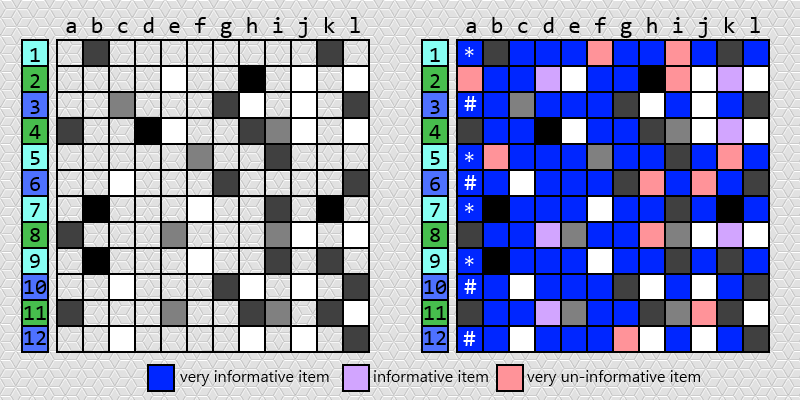
\includegraphics[width=\textwidth]{RS-ALdiag}
    \else
      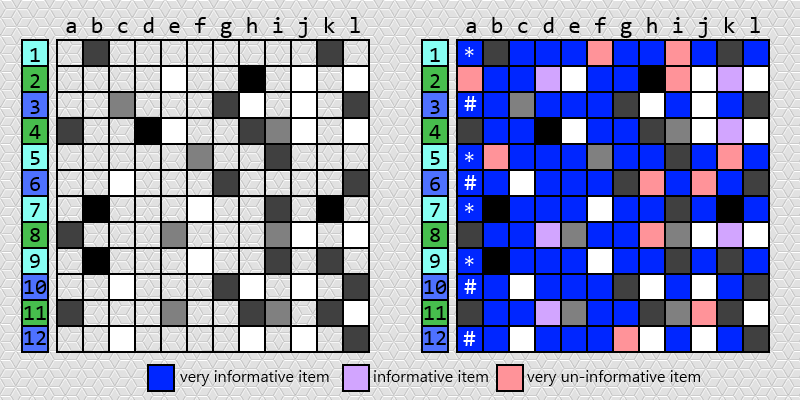
\includegraphics[bb = 92 86 545 742, width=\textwidth]{RS-ALdiag}
    \fi
    \end{center}
Users are represented in rows, and there has been 3 type of users defined, dark blue, light blue and green. Items are represented in the columns by letters. User item pairs that are rated are represented by a shade of grey and unrated squares are left blank.
    \caption{Diagram of a simplified user-item matrix used for recommender systems}
    \label{fig:al-diag}
\end{figure}

Figure \ref{fig:al-diag} gives us a very simplified graphical explanation of what an active learning system can achieve. To the left we have a sparse user-item matrix, each coloured square represents a rating, with the intensity representing a rating or interaction (for example black could represent 4, dark grey 3, light grey 2 and white 1). To simplify, we can assume that the system has recognised that there are 3 types of user groups, light blue, dark blue and green. Each of these user groups have the same interests. Using a film database analogy, a green user could be an action movie fan whereas light blue users could be comedy aficionados. Thus if it needed to predict what the rating \texttt{a2} would be, extra sampling would not really be useful as we know \texttt{a4}, \texttt{a8} and \texttt{a11}, which are all part of the green group. Knowing \texttt{a2}, along with \texttt{b5} and other pink ratings (from the right matrix) is of little use. However knowing just one of \texttt{a1-5-7-9} and \texttt{a3-6-10-12} is very useful as it gives us a rough idea as to what light and dark blue users think of item \texttt{a}. Collecting samples for users we already have a reasonably good profile of only helps us improve the certainty of certain ratings rather than be able to say something new about the dataset. Again it may be the case that the item rating isn't the same for one user group but this is an idealistic scenario.


\section{Measuring Effectiveness}
Determining whether or not a sampling method is effective or not is mainly a matter of seeing how well it impacts the performance. For example if the average sample added to a model leads to a 0.01 RMSE decrease and we can select the ones leading to 0.02 RMSE decrease on average then it can be said that this is effective. The benchmark case is defined to be random sampling, that is choosing a new sample at random. As random sampling may select an informative sample just as well as a less useful one, many random sampling trials must be done and averaged together to see the expected random performance. The benchmark RMSE for random sampling can be seen in the appendix figure \ref{fig:RandomPMF}. This is because one random sampling instance may outperform a poor active sampling method. Figure \ref{fig:al_minknowl} shows a case of random sampling performing as well or outperforming an active sampling method (in this case this is a basic one developed for this project called minimum knowledge search).

\begin{figure}[!htbp]
  \begin{center}
    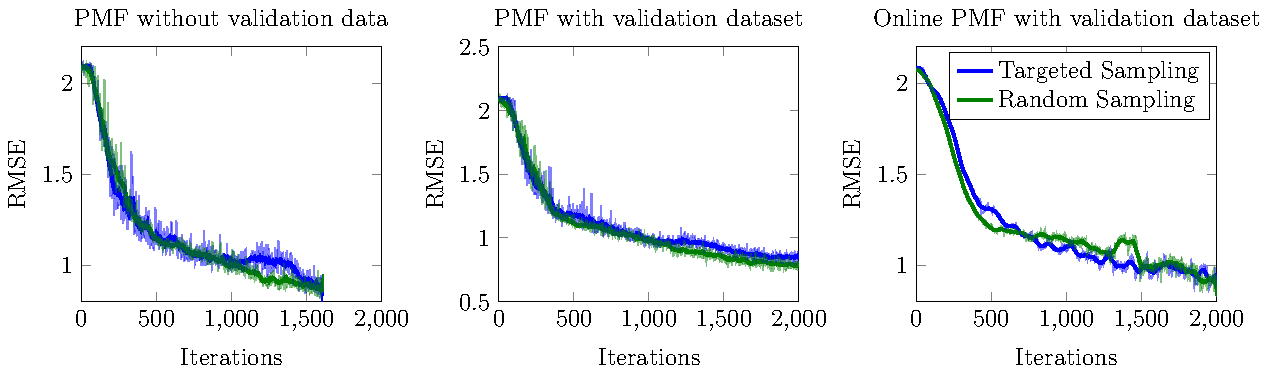
\includegraphics[width=\textwidth]{min_knowl_rate}
    Each iteration involves the discovery of one new sample. Dataset is the synthetic one from figure \ref{fig:5pcmat}.
    \caption{Active Sampling trial for the "minimum knowledge" selection}
    \label{fig:al_minknowl}
  \end{center}
\end{figure}

Another measure of the active sampling algorithm is to compare the area under the curve of the RMSE over the number of discovered samples. This measure gives an idea of what total advantage the targeted sampling may have.



It is important to be consistent with what model is used to predict data as some samples may be more useful for one model than an another. For example one model, like BPMF, will perform well by knowing a bit of everything to infer a posterior distribution of data, however PMF which does not do this will not find this sample as useful.

Effectiveness could also be linked to individual RMSE decrease, that is when a sample is discovered the amount by which it has decreased RMSE is used to rate how useful it has been. This can be a somewhat subjective error as the more about a model is know the harder RMSE decrease is.

\subsection{Discrete vs Continuous Data}
RMSE will be different for discrete and continuous data due to the way it is post-processed. Continuous data, obtained from $\hat{R}=U^TV$, is left untouched and used to calculate RMSE. For discrete data the values of $\hat{R}$ are first bounded between the minimum and maximum, for example 1 and 5 for film ratings. After this $\hat{R}$ is rounded to the nearest number in the discrete set. Error can then be calculate as traditional RMSE or as number of correct(sometimes referred to as positive) samples \cite{recsyshand}.
\section{Formal Definition}
The mask matrix $Z$ is used to determine whether a value is known (or more accurately, part of the training set, the training set mask is called $Z_{tr}$). Its indices are the same as $R$ except that values can only be $0$ or $1$. The known values are represented by $1$ and form the set $\mathcal{O}$. In other words $R_\mathcal{O}$ is the matrix of the known values. We will also have the pool of queriable samples $\mathcal{P}$, that is the samples not yet known but that may be requested. Note that it is not always the case that $R_{\mathcal{O}} \cap R_{\mathcal{P}} = R$ as there may be unqueriable unknown samples. The samples queried part of the active sampling process will form the set $\mathcal{A}$, with $R_{\mathcal{A}}$ being the requested values. In graphical form the matrix representing $\mathcal{A}$ will usually be coloured. White represents the unrequested samples and the coloured cells represent the order of sampling.


\section{Goals of Active Sampling}
\label{sec:as_goals}
To select certain samples some aspects which are thought to be able to reduce RMSE better than random selection are outlined.

\begin{description}[style=standard,leftmargin=.7cm,font=\bfseries]
  \item[Model] Look at samples that may produce the greatest change in the parameters $U$ and $V$, with he hope that this will mean a large change towards the true distribution.
  \item[Sample Uncertainty] Try to seek the samples that are most likely to vary based on current distribution of parameters, that is their uncertainty.
  \item[Knowledge] How much is known about a current row or column and aiming to maximise this overall, with the aim of getting a global insight of the data.
  \item[Max-Minimum] To best determine the boundaries of the data the largest and smallest estimated values are queried with the aim of minimising over and under estimation error.
\end{description}


\section{Minimum Knowledge Search}
\label{sec:mks_alg}
%\markboth{\MakeUppercase{\thechapter. My Second Chapter }}
Before looking at advanced sampling techniques a basic one was made to illustrate the concepts and basic increase in performance possible.
\subsection{Algorithm}
For any matrix factorisation problem we have the mask matrix $Z \in \mathbb{R}^{M \times N}$, with elements being 1 for every known value and 0 for every unknown value (values in the validation set would be also 0).

\begin{algorithm}
\caption{Minimum Knowledge Search algorithm}\label{alg:min_knowl}
\begin{algorithmic}[1]
\Procedure{MinKnowSearch}{$Z$}\Comment{The mask matrix as input}
\State $\mathbf{a} \gets \text{meanrow}(Z)$ \Comment{Mean of rows, $\mathbf{a} \in \mathbb{R}^N$}
\State $\mathbf{b} \gets \text{meancol}(Z)$ \Comment{Mean of columns, $\mathbf{b} \in \mathbb{R}^M$}
\State $K \gets \mathbf{a} \cdot \mathbf{b}$ \Comment{ $K \in \mathbb{R}^{M\times N}$}
\State $x,y \gets index\_of\_min(K)$ \Comment{Often multiple candidates, select first one}
\While{$Z(x,y)==1$}\Comment{Also check for validation mask}
\State $x,y \gets next\_min\_index(K)$
\EndWhile
\State \textbf{return} $x,y$\Comment{Return $x,y$ that has least knowledge}
\EndProcedure
\end{algorithmic}
\end{algorithm}

Knowing a bit about each column and row is a good first step to discover more about a matrix. This is the motivation of creating a heatmap of what we know about each cell. To do this we take the mean of the row and columns of $Z$. Say $\mathbf{a}=meanrow(Z)$ and $\mathbf{b}=meancolumn(Z)$. This defines the amount known for each row and column - i.e. if $\mathbf{a}_i = 0$ then there is no known sample of row $i$, if $\mathbf{b}_j = 1$ then we know all samples of column $j$. From this we can get a knowledge matrix $K= \mathbf{a} \cdot \mathbf{b}$, which acts as a heatmap of what is known of $R$. From this we can find the cells with the minimum values and target them. There will often be multiple cells of lower value but not all may be available. For example it may be impossible to sample them or it may be a cell in the validation set. For this reason we select the lowest compatible cell. The full algorithm is described in algorithm \ref{alg:min_knowl}.

\begin{figure}[!htbp]
  \begin{center}
    \resizebox{\textwidth}{!}{% This file was created by matlab2tikz v0.4.7 running on MATLAB 8.1.
% Copyright (c) 2008--2014, Nico Schlömer <nico.schloemer@gmail.com>
% All rights reserved.
% Minimal pgfplots version: 1.3
% 
% The latest updates can be retrieved from
%   http://www.mathworks.com/matlabcentral/fileexchange/22022-matlab2tikz
% where you can also make suggestions and rate matlab2tikz.
% 
\begin{tikzpicture}

\begin{axis}[%
width=2.5in,
height=2.75in,
axis on top,
scale only axis,
xmin=0.5,
xmax=50.5,
y dir=reverse,
ymin=0.5,
ymax=80.5,
name=plot2,
title={Knowledge Matrix $K$}
]
\addplot [forget plot] graphics [xmin=0.5,xmax=50.5,ymin=0.5,ymax=80.5] {search_mat-1.png};
\end{axis}

\begin{axis}[%
width=2.5in,
height=2.75in,
axis on top,
scale only axis,
xmin=0.5,
xmax=50.5,
y dir=reverse,
ymin=0.5,
ymax=80.5,
at=(plot2.left of south west),
anchor=right of south east,
title={Known Samples $Z \in \mathbb{R}^{M \times N}$}
]
\addplot [forget plot] graphics [xmin=0.5,xmax=50.5,ymin=0.5,ymax=80.5] {search_mat-2.png};
\end{axis}

\begin{axis}[%
width=.25in,
height=2.75in,
axis on top,
scale only axis,
%xmin=0.5,
%xmax=1.5,
xticklabels={,,},
%y dir=reverse,
ymin=0.5,
ymax=50.5,
name=plot3,
at=(plot2.right of south east),
anchor=left of south west
]
\addplot [forget plot] graphics [xmin=0,xmax=1,ymin=0.5,ymax=50.5] {search_mat-3.png};
\end{axis}

\begin{axis}[%
width=2.5in,
height=2.75in,
axis on top,
scale only axis,
xmin=0.5,
xmax=50.5,
y dir=reverse,
ymin=0.5,
ymax=80.5,
at=(plot3.right of south east),
anchor=left of south west,
title={Search Matrix}
]
\addplot [forget plot] graphics [xmin=0.5,xmax=50.5,ymin=0.5,ymax=80.5] {search_mat-4.png};
\end{axis}
\end{tikzpicture}%}
  \end{center}
  The darker the colour in the knowledge matrix, the least is known about that cell due to the column-row combination.
    \caption{Diagram of initial parameters and search path}
    \label{fig:min_know_search}
\end{figure}

Figure \ref{fig:min_know_search} illustrates the way minimum knowledge search works. From the known samples we see that the knowledge matrix has many "low knowledge" areas (in dark blue) to select from. A sequence of 200 sample selections is shown on the rightmost image. The first samples are blue in color, tending to red as the final samples are targeted (as shown by the colour legend to the left of it). As we see it selects the least known elements in the first row then column first. The pattern is due to selecting the very first possible least known element - a variant would be to randomly select an element to potentially try and get a temporary advantage.

\textit{Note:} Other variants of this algorithm that were tried included selecting the minimum suitable index of $\mathbf{a}$ and $\mathbf{b}$ - i.e. the coordinates that intersect with the least known row and column. However this technique did not perform as well due to not seeking to maximise one row and column first at the start. The random minimum knowledge matrix selection variant also suffers from this.


\subsection{Notes on performance}

To better compare sampling algorithms we benchmark them against random sampling by defining the advantage value as 
\begin{align*}
\frac{\text{RMSE Area under random selection}}{\text{RMSE Area under targeted selection}}
\end{align*}


\begin{figure}[!htbp]
  \begin{center}
    \resizebox{\textwidth}{!}{% This file was created by matlab2tikz v0.4.7 running on MATLAB 8.1.
% Copyright (c) 2008--2014, Nico Schlömer <nico.schloemer@gmail.com>
% All rights reserved.
% Minimal pgfplots version: 1.3
% 
% The latest updates can be retrieved from
%   http://www.mathworks.com/matlabcentral/fileexchange/22022-matlab2tikz
% where you can also make suggestions and rate matlab2tikz.
% 
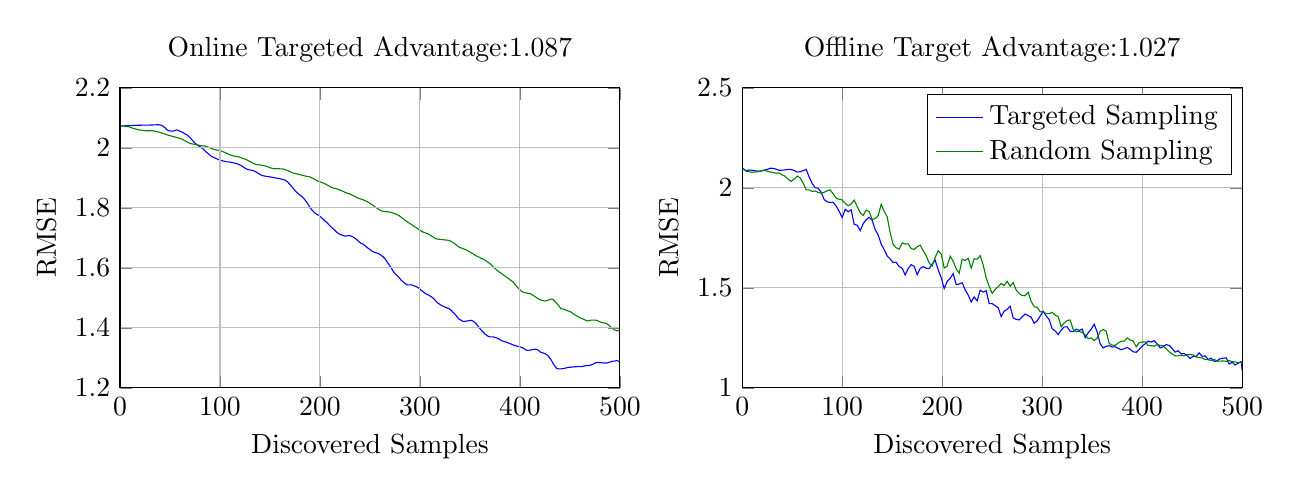
\begin{tikzpicture}

\begin{axis}[%
width=2.5in,
height=1.5in,
axis on top,
scale only axis,
xmin=0,
xmax=500,
xlabel={Discovered Samples},
xmajorgrids,
ymin=1.2,
ymax=2.2,
ylabel={RMSE},
ymajorgrids,
name=plot2,
title={Online Targeted Advantage:1.087}
]
\addplot [color=blue,solid,forget plot]
  table[row sep=crcr]{1	2.07310604133759\\
3	2.07326671713631\\
5	2.07357900586304\\
7	2.07388454435722\\
9	2.07413520970242\\
11	2.07442055079419\\
13	2.07468552217153\\
15	2.07495763872169\\
17	2.07517479065046\\
19	2.07541279796415\\
21	2.07552681878607\\
23	2.07567554770087\\
25	2.07574842378073\\
27	2.0758351989298\\
29	2.07601197081117\\
31	2.07624426489261\\
33	2.07640751446076\\
35	2.07668859545529\\
37	2.07700457165685\\
39	2.07733472347428\\
41	2.07547584678732\\
43	2.07267437054161\\
45	2.06719425000654\\
47	2.06045449193378\\
49	2.05704843627313\\
51	2.05622179611769\\
53	2.05559423696112\\
55	2.05798565857626\\
57	2.06001165822928\\
59	2.05672667279463\\
61	2.05441791887093\\
63	2.05079338565582\\
65	2.04704134065486\\
67	2.0432464385897\\
69	2.03767594564495\\
71	2.03080465916258\\
73	2.02332466132037\\
75	2.01606511084671\\
77	2.01050836397315\\
79	2.00600177919479\\
81	2.00207646759487\\
83	1.99674907672468\\
85	1.99004841108889\\
87	1.98406230282771\\
89	1.97900396970908\\
91	1.97256442314763\\
93	1.96946098036203\\
95	1.96642629748446\\
97	1.96337100951813\\
99	1.96038831260488\\
101	1.95815696385899\\
103	1.95638732161264\\
105	1.95468169501334\\
107	1.95357209186961\\
109	1.95305916135409\\
111	1.95184558004146\\
113	1.95045062137535\\
115	1.94894180782721\\
117	1.94733170690149\\
119	1.94449810032508\\
121	1.94145719906061\\
123	1.93721860458704\\
125	1.93261215856807\\
127	1.928900820703\\
129	1.92696944278035\\
131	1.92571495682112\\
133	1.92442479753473\\
135	1.9219685297118\\
137	1.91798018780745\\
139	1.91375563422737\\
141	1.90965903286238\\
143	1.90705998351704\\
145	1.905924351467\\
147	1.90459694248099\\
149	1.90378962343441\\
151	1.90281136704651\\
153	1.90115254618828\\
155	1.89997381696884\\
157	1.89896582484351\\
159	1.89769006901247\\
161	1.89642054022761\\
163	1.89480113466052\\
165	1.89259634741089\\
167	1.88858193219726\\
169	1.88140951305761\\
171	1.87415627460295\\
173	1.86647177694502\\
175	1.85775278240807\\
177	1.85127347700434\\
179	1.84584684421737\\
181	1.84002596175315\\
183	1.8346474166887\\
185	1.82673564948299\\
187	1.81786732647924\\
189	1.80720989947165\\
191	1.79704968680991\\
193	1.78919071530109\\
195	1.78254362882129\\
197	1.77865600407582\\
199	1.77449187926219\\
201	1.76918447147305\\
203	1.7629513941636\\
205	1.75651116970766\\
207	1.75149701009629\\
209	1.74332521729506\\
211	1.73676357113323\\
213	1.73087441735158\\
215	1.72489402787526\\
217	1.71814668294055\\
219	1.7135034789444\\
221	1.71056025906535\\
223	1.70786032246719\\
225	1.70594703893975\\
227	1.7064549179845\\
229	1.70807128247458\\
231	1.70605250584992\\
233	1.70312810539291\\
235	1.6988038168626\\
237	1.69329117085346\\
239	1.68705328798764\\
241	1.68182250636833\\
243	1.67963830038975\\
245	1.67427709968178\\
247	1.66841765463489\\
249	1.66358120989105\\
251	1.65840680159531\\
253	1.65381938848512\\
255	1.65120784910666\\
257	1.64960980153934\\
259	1.64719710037129\\
261	1.64236248029456\\
263	1.6372697043131\\
265	1.6305726585535\\
267	1.62103791792682\\
269	1.61081741702213\\
271	1.60121859066473\\
273	1.59010524580202\\
275	1.58088894946804\\
277	1.57515369253082\\
279	1.56853535308195\\
281	1.55984905705212\\
283	1.55345652263816\\
285	1.54825474217291\\
287	1.54366424047559\\
289	1.54334466460373\\
291	1.54360121997258\\
293	1.5417615920569\\
295	1.53934629418234\\
297	1.53640636314194\\
299	1.53194037094738\\
301	1.52632904431432\\
303	1.52108820369212\\
305	1.51562303243172\\
307	1.51160799635526\\
309	1.50891484650005\\
311	1.50422634621712\\
313	1.4997213453529\\
315	1.49290263640234\\
317	1.48500633147118\\
319	1.48039968308882\\
321	1.47551031245921\\
323	1.47218314734148\\
325	1.46942252162529\\
327	1.46682488606447\\
329	1.46401748046693\\
331	1.45893077258082\\
333	1.45211345526009\\
335	1.44610464082881\\
337	1.43769925190376\\
339	1.42911316167982\\
341	1.42586829841142\\
343	1.42174872679996\\
345	1.4214296918236\\
347	1.42332220005112\\
349	1.4236563895757\\
351	1.42534453017348\\
353	1.42321065405664\\
355	1.41751953701089\\
357	1.41054200072895\\
359	1.40219266832331\\
361	1.39329254132761\\
363	1.38637121611743\\
365	1.37964942139744\\
367	1.37478934480892\\
369	1.37057644950698\\
371	1.36980021255196\\
373	1.37016578268997\\
375	1.36849878544926\\
377	1.36600312508128\\
379	1.36317789593027\\
381	1.35855002160093\\
383	1.35561418417972\\
385	1.35344425555225\\
387	1.35185296943341\\
389	1.34882878450625\\
391	1.34627502381213\\
393	1.3436214481878\\
395	1.34098246428187\\
397	1.33921814362833\\
399	1.33820071413604\\
401	1.3354915618712\\
403	1.3330208174832\\
405	1.32868815157956\\
407	1.32484813178625\\
409	1.32507458826941\\
411	1.32664010835803\\
413	1.32798295074099\\
415	1.32903727816498\\
417	1.3282399154655\\
419	1.32359490486935\\
421	1.31842904260654\\
423	1.31639869325332\\
425	1.31414661928195\\
427	1.31018634608281\\
429	1.30341378448534\\
431	1.29460767232202\\
433	1.2821770172429\\
435	1.27232536557794\\
437	1.2645582533132\\
439	1.26313548931517\\
441	1.26337388673075\\
443	1.26431047268404\\
445	1.26546456951398\\
447	1.26725718514147\\
449	1.26876682904483\\
451	1.26885628670924\\
453	1.26961787462963\\
455	1.27037995920581\\
457	1.27068347516571\\
459	1.27078690497629\\
461	1.27083685399705\\
463	1.27166414782999\\
465	1.27345911263117\\
467	1.2741474168869\\
469	1.27434088523759\\
471	1.27651748043922\\
473	1.27875119564344\\
475	1.28247518214614\\
477	1.28468612076\\
479	1.28436084815503\\
481	1.28392412046332\\
483	1.28347928549919\\
485	1.28277225370072\\
487	1.28319989413008\\
489	1.28512421343161\\
491	1.28725828246269\\
493	1.28901363374399\\
495	1.28936602600243\\
497	1.29156219174095\\
499	1.28772549126402\\
500	1.28852400740035\\
};
\addplot [color=black!50!green,solid,forget plot]
  table[row sep=crcr]{1	2.07273486064028\\
3	2.07269718381591\\
5	2.07207773367045\\
7	2.07136282740526\\
9	2.07027448149238\\
11	2.06786230875929\\
13	2.06534441128157\\
15	2.06356333901095\\
17	2.06173328791467\\
19	2.06004227573472\\
21	2.05910548214283\\
23	2.05838424784717\\
25	2.05755798942924\\
27	2.05693269060563\\
29	2.0571709027592\\
31	2.05710941025419\\
33	2.05691498078809\\
35	2.05543771802835\\
37	2.05390367098843\\
39	2.05243943323188\\
41	2.05046108144473\\
43	2.04851158507928\\
45	2.0462022301676\\
47	2.04373646038315\\
49	2.04142481195887\\
51	2.03999919717474\\
53	2.03821157131603\\
55	2.03634853447946\\
57	2.03450626193127\\
59	2.0324709318215\\
61	2.03019705854381\\
63	2.02762814112215\\
65	2.02372983225735\\
67	2.01992164605917\\
69	2.01631269543438\\
71	2.01387316909839\\
73	2.01292768341919\\
75	2.01159687681705\\
77	2.01017193053528\\
79	2.00876764141652\\
81	2.0073175826654\\
83	2.00673400558414\\
85	2.00621494530757\\
87	2.00433376110501\\
89	2.00153619376714\\
91	1.99899125789614\\
93	1.9958294536442\\
95	1.99378977562286\\
97	1.99287231771115\\
99	1.99174488329168\\
101	1.98989301514239\\
103	1.9874859182881\\
105	1.98457721799165\\
107	1.98133411090366\\
109	1.97823871999702\\
111	1.97597888954311\\
113	1.97362908642283\\
115	1.97215187691542\\
117	1.97110251152674\\
119	1.96986189620474\\
121	1.96757155142401\\
123	1.96495689005109\\
125	1.96255143277317\\
127	1.96004569234656\\
129	1.95600702804609\\
131	1.95263731729457\\
133	1.94930393616194\\
135	1.94579517351422\\
137	1.9440219663311\\
139	1.94345924332638\\
141	1.94283532669952\\
143	1.9414643778858\\
145	1.93979929500294\\
147	1.93795540880696\\
149	1.93537415868857\\
151	1.93275895518515\\
153	1.93119726760837\\
155	1.93027734756375\\
157	1.93089373361375\\
159	1.93040045064236\\
161	1.92991454517862\\
163	1.92966004755571\\
165	1.92780129287495\\
167	1.92516480255259\\
169	1.9228116766269\\
171	1.91929104747833\\
173	1.91646847257185\\
175	1.91470426541642\\
177	1.91337976250874\\
179	1.91140772177429\\
181	1.90976391854329\\
183	1.90803981477576\\
185	1.90629695418856\\
187	1.90502081613502\\
189	1.903867372766\\
191	1.90165381329393\\
193	1.89840061356952\\
195	1.89454538088788\\
197	1.89080151856267\\
199	1.88760243532117\\
201	1.88578372128689\\
203	1.88298865851811\\
205	1.88024772260958\\
207	1.87681445170193\\
209	1.87303303950111\\
211	1.86911132960192\\
213	1.86636849750195\\
215	1.86462220722285\\
217	1.86331721169568\\
219	1.86053664743174\\
221	1.85798543831125\\
223	1.85548032151616\\
225	1.85190192536975\\
227	1.84936981877731\\
229	1.84741729078074\\
231	1.84477851681337\\
233	1.84119975342469\\
235	1.83771053918094\\
237	1.83430110402774\\
239	1.83155403929362\\
241	1.82918012653496\\
243	1.82719096966126\\
245	1.82419052244626\\
247	1.82119461975891\\
249	1.81727876511456\\
251	1.81253065789519\\
253	1.80886950779078\\
255	1.80425444679067\\
257	1.79916320501629\\
259	1.79444314818509\\
261	1.79134966250026\\
263	1.78869236256182\\
265	1.78736620048557\\
267	1.78712276571121\\
269	1.78658647730534\\
271	1.78483057407413\\
273	1.78264039788359\\
275	1.78052656980415\\
277	1.77740890983066\\
279	1.77451075306677\\
281	1.76924177249018\\
283	1.76420485369328\\
285	1.7589703598607\\
287	1.75429573859356\\
289	1.74991752472778\\
291	1.74558496165372\\
293	1.74108665583289\\
295	1.73649922694422\\
297	1.73260272536152\\
299	1.72742959923414\\
301	1.72358635766568\\
303	1.71962667584446\\
305	1.71720749911194\\
307	1.71483821299807\\
309	1.71176314116979\\
311	1.70728771832818\\
313	1.70335716048384\\
315	1.69882950335931\\
317	1.69628082535797\\
319	1.69527400934709\\
321	1.69491454482463\\
323	1.69397986357916\\
325	1.69316745473562\\
327	1.6927036066882\\
329	1.6914198932547\\
331	1.6886754428624\\
333	1.68494020500824\\
335	1.68005185496385\\
337	1.67416676625924\\
339	1.66969183991548\\
341	1.6668683040587\\
343	1.66397991920486\\
345	1.66147417376529\\
347	1.65906488942949\\
349	1.65525448066485\\
351	1.65065993029129\\
353	1.64727554951556\\
355	1.64252438564956\\
357	1.63882912730723\\
359	1.63602548617199\\
361	1.63200619424515\\
363	1.62948769076905\\
365	1.62565402111873\\
367	1.62132406834684\\
369	1.61695186847789\\
371	1.61101443180133\\
373	1.60415832438942\\
375	1.59851020796185\\
377	1.59217142296305\\
379	1.58673395734103\\
381	1.58252731088254\\
383	1.57780113026447\\
385	1.57286972547394\\
387	1.56840709394255\\
389	1.56313388791699\\
391	1.5582048828967\\
393	1.55331482357838\\
395	1.54520145783292\\
397	1.53728310651685\\
399	1.52993433356511\\
401	1.52371164110378\\
403	1.51958812343301\\
405	1.5172891526535\\
407	1.51577380981124\\
409	1.51468393953684\\
411	1.51317678444096\\
413	1.50867049372451\\
415	1.50470933432015\\
417	1.49994949606754\\
419	1.49540387377287\\
421	1.49269844866819\\
423	1.4909014464262\\
425	1.48962769543592\\
427	1.49072174272157\\
429	1.49355732074938\\
431	1.49591547834098\\
433	1.49478794974311\\
435	1.48802152015223\\
437	1.48072511194826\\
439	1.47324294134576\\
441	1.46386363227968\\
443	1.46312090117667\\
445	1.46065877443958\\
447	1.45796725612642\\
449	1.45569724049918\\
451	1.45287798998927\\
453	1.44764756061492\\
455	1.44333827238177\\
457	1.43945794536372\\
459	1.43575893140027\\
461	1.43193963415499\\
463	1.42975866882633\\
465	1.42655364396775\\
467	1.42306743343297\\
469	1.42402017484595\\
471	1.42553586963352\\
473	1.42603146555452\\
475	1.42608032701067\\
477	1.42484323113859\\
479	1.42158070572272\\
481	1.41895651444658\\
483	1.41701295189395\\
485	1.41587636236088\\
487	1.41343810856089\\
489	1.40851427344181\\
491	1.40244372478748\\
493	1.39687537335943\\
495	1.39282856164765\\
497	1.38999068219996\\
499	1.39150679218542\\
500	1.39030254853776\\
};
\end{axis}

\begin{axis}[%
width=2.5in,
height=1.5in,
scale only axis,
xmin=0,
xmax=500,
xlabel={Discovered Samples},
xmajorgrids,
ymin=1,
ymax=2.5,
ylabel={RMSE},
ymajorgrids,
at=(plot2.right of south east),
anchor=left of south west,
title={Offline Target Advantage:1.027},
legend style={draw=black,fill=white,legend cell align=left}
]
\addplot [color=blue,solid]
  table[row sep=crcr]{1	2.09623558837252\\
4	2.08557349037409\\
7	2.08941881915104\\
10	2.08810235513169\\
13	2.08528717647888\\
16	2.08368014315202\\
19	2.08349698341216\\
22	2.08898947634742\\
25	2.09236980810638\\
28	2.09796306515968\\
31	2.09777717202992\\
34	2.09303393262892\\
37	2.08777634564646\\
40	2.08852121436469\\
43	2.08995827267659\\
46	2.09256803234949\\
49	2.09169930356983\\
52	2.08658620882621\\
55	2.07945768763512\\
58	2.08068089042345\\
61	2.08621291062325\\
64	2.09258212001829\\
67	2.0542058818581\\
70	2.02210523804509\\
73	2.00033493183981\\
76	1.9981335625122\\
79	1.97872236741582\\
82	1.94140003217971\\
85	1.93060632291208\\
88	1.92687580167824\\
91	1.928208650656\\
94	1.90819705872971\\
97	1.88247183915474\\
100	1.85203041700107\\
103	1.89263828462933\\
106	1.88064430604419\\
109	1.89004831396205\\
112	1.81776837072684\\
115	1.81356653937725\\
118	1.7866644793684\\
121	1.82130467528387\\
124	1.84066550456028\\
127	1.85257625605776\\
130	1.83778378268688\\
133	1.79090500800056\\
136	1.76504190122341\\
139	1.71852334723789\\
142	1.69138855831463\\
145	1.65955104916942\\
148	1.64374996416446\\
151	1.62700545978928\\
154	1.62805841327501\\
157	1.60640282197778\\
160	1.59796309510609\\
163	1.56461229076778\\
166	1.5969255240773\\
169	1.61589295020528\\
172	1.60800140768756\\
175	1.56560748860849\\
178	1.59733589863452\\
181	1.60631219378402\\
184	1.59836503478009\\
187	1.59677922141894\\
190	1.61938847478455\\
193	1.63833230002915\\
196	1.5902394680023\\
199	1.55128520425811\\
202	1.49691177252886\\
205	1.53267550874508\\
208	1.5481229318826\\
211	1.57147425283505\\
214	1.51701589379702\\
217	1.51882054354361\\
220	1.52599256965096\\
223	1.48967665748365\\
226	1.46492482452034\\
229	1.42963487207446\\
232	1.45454414118878\\
235	1.43538311769399\\
238	1.48860176991854\\
241	1.47881243482667\\
244	1.48558190138466\\
247	1.42162604238114\\
250	1.42131112364471\\
253	1.41097835412453\\
256	1.40075480194048\\
259	1.35648946186223\\
262	1.38293641189566\\
265	1.39351226437504\\
268	1.40806431121776\\
271	1.35003740901968\\
274	1.34234875204519\\
277	1.33980333293141\\
280	1.35540243532046\\
283	1.3695812506518\\
286	1.36071571972052\\
289	1.3536985677449\\
292	1.32311148211838\\
295	1.3353322909363\\
298	1.35957413603505\\
301	1.38329491469548\\
304	1.35938035748346\\
307	1.34144645254962\\
310	1.2958979364115\\
313	1.28451415338732\\
316	1.26630672359156\\
319	1.28862354037248\\
322	1.304650178528\\
325	1.30531679354453\\
328	1.28296408867899\\
331	1.28104188752466\\
334	1.29338045409757\\
337	1.28709680143707\\
340	1.2937556124161\\
343	1.25093754566392\\
346	1.27542438464222\\
349	1.29367672538461\\
352	1.31831032055013\\
355	1.27927958090711\\
358	1.22050829708344\\
361	1.19968072447957\\
364	1.20787413555955\\
367	1.21125886047017\\
370	1.20425280652824\\
373	1.20560249522302\\
376	1.19777809597297\\
379	1.19047173137184\\
382	1.19593798976182\\
385	1.20219234974779\\
388	1.19279268203412\\
391	1.18048591479491\\
394	1.17788785225877\\
397	1.19214086630369\\
400	1.20946196406756\\
403	1.22018549445231\\
406	1.23363888661019\\
409	1.22894652874213\\
412	1.23645543338356\\
415	1.22008915667504\\
418	1.20018135249687\\
421	1.2059073531626\\
424	1.21664376577866\\
427	1.21215117662033\\
430	1.19732051507061\\
433	1.1788061330717\\
436	1.18561560279885\\
439	1.17002411488917\\
442	1.17183737388939\\
445	1.16173419562447\\
448	1.14694528339278\\
451	1.1584418315822\\
454	1.15718890613823\\
457	1.17530476412869\\
460	1.15760458870801\\
463	1.16009324205582\\
466	1.14169100000451\\
469	1.1483717150176\\
472	1.13258990901309\\
475	1.13555122302965\\
478	1.14616568657655\\
481	1.14836757627439\\
484	1.15029284211486\\
487	1.11937892444902\\
490	1.12839908103115\\
493	1.11417433212312\\
496	1.12341215670216\\
499	1.13107448027654\\
500	1.08668410908653\\
};
\addlegendentry{Targeted Sampling};

\addplot [color=black!50!green,solid]
  table[row sep=crcr]{1	2.09501172349217\\
4	2.08293870028101\\
7	2.08045379104404\\
10	2.07804993771589\\
13	2.07960926239589\\
16	2.08070758961635\\
19	2.08659654329752\\
22	2.08698059751515\\
25	2.08372191822112\\
28	2.07958988226961\\
31	2.07717778867386\\
34	2.0729447617295\\
37	2.07435901201342\\
40	2.06506462372548\\
43	2.05782756707244\\
46	2.0431666551047\\
49	2.03273931655845\\
52	2.04398815532092\\
55	2.05846140897223\\
58	2.04975864740821\\
61	2.02341162058181\\
64	1.98995433096665\\
67	1.99010890763763\\
70	1.98217891559289\\
73	1.98471274698831\\
76	1.97696137891592\\
79	1.97394935088951\\
82	1.97825743949756\\
85	1.98556259020551\\
88	1.99021035616647\\
91	1.96983766458318\\
94	1.94825841505483\\
97	1.94307209454356\\
100	1.93971453711601\\
103	1.92259485112982\\
106	1.91054335163527\\
109	1.91990824388004\\
112	1.93881315150296\\
115	1.90726268821967\\
118	1.87568821474338\\
121	1.86240064198228\\
124	1.8886402936451\\
127	1.88125116194824\\
130	1.84217791750189\\
133	1.8465042475188\\
136	1.86124269972939\\
139	1.91841606935752\\
142	1.88243201685829\\
145	1.85522441497156\\
148	1.77571870088768\\
151	1.71629539737682\\
154	1.70038322564714\\
157	1.69335511504176\\
160	1.72499588414554\\
163	1.71951511280064\\
166	1.71996542736959\\
169	1.69687223969179\\
172	1.69204457145387\\
175	1.70583018895992\\
178	1.71370884781952\\
181	1.68624132316335\\
184	1.66077403131635\\
187	1.62406406009842\\
190	1.609710112789\\
193	1.65272336588136\\
196	1.68579688066345\\
199	1.66879896851576\\
202	1.59965096673837\\
205	1.60885655719668\\
208	1.65859130548986\\
211	1.63368404741668\\
214	1.59538008534167\\
217	1.57296508833288\\
220	1.64333960214517\\
223	1.63704548741144\\
226	1.64755931922927\\
229	1.59855720305325\\
232	1.64576301295597\\
235	1.64328708688335\\
238	1.6610194350617\\
241	1.61510744865109\\
244	1.54947336430295\\
247	1.50760947759938\\
250	1.47231274285789\\
253	1.49308164602425\\
256	1.50615944196781\\
259	1.52168372612609\\
262	1.51213674885728\\
265	1.53277361500399\\
268	1.50788835084955\\
271	1.52670131041786\\
274	1.48897024187698\\
277	1.47228626179601\\
280	1.46115631482788\\
283	1.46078239963633\\
286	1.47790905368603\\
289	1.43232005406434\\
292	1.40568503277145\\
295	1.4028853987067\\
298	1.38078336394117\\
301	1.37987703280474\\
304	1.37160939503333\\
307	1.37098711603995\\
310	1.3780306759949\\
313	1.36365060159499\\
316	1.35632478725668\\
319	1.30524682081509\\
322	1.32496668875371\\
325	1.33705005462304\\
328	1.33943336108902\\
331	1.29172086141883\\
334	1.2805294706101\\
337	1.28239383509277\\
340	1.27719896562986\\
343	1.26573281850245\\
346	1.2464588393257\\
349	1.2497762588219\\
352	1.23696939355274\\
355	1.24796094031928\\
358	1.28275420364581\\
361	1.29192354645752\\
364	1.28346042815004\\
367	1.22198827043422\\
370	1.21372420348027\\
373	1.21250865874745\\
376	1.22433469913556\\
379	1.23306009853477\\
382	1.23412430492534\\
385	1.25025601339111\\
388	1.23925302577228\\
391	1.23448273107499\\
394	1.20543006731131\\
397	1.22599463503145\\
400	1.22896913685223\\
403	1.23029987714075\\
406	1.21157092252635\\
409	1.21060074776435\\
412	1.20843389564234\\
415	1.21688722820609\\
418	1.21237602156283\\
421	1.21096931775804\\
424	1.19484119909435\\
427	1.17998872640249\\
430	1.1693634680154\\
433	1.16046738879857\\
436	1.16019442991082\\
439	1.1636002745657\\
442	1.15998304862206\\
445	1.16687269643565\\
448	1.16703518583644\\
451	1.16453964363033\\
454	1.15409859651281\\
457	1.15155556156158\\
460	1.14989801984772\\
463	1.14125214893952\\
466	1.14110841823961\\
469	1.13656250413446\\
472	1.14257239295239\\
475	1.13306781671376\\
478	1.13394865406197\\
481	1.134749468441\\
484	1.13246745227602\\
487	1.13675870768403\\
490	1.13064794801889\\
493	1.13005967021843\\
496	1.12577638968963\\
499	1.12964183605538\\
500	1.12000525208853\\
};
\addlegendentry{Random Sampling};

\end{axis}
\end{tikzpicture}%}
  \end{center}
  Over 10 online trials, minimum knowledge search advantage was $1.043$. Final random RMSE:1.390, targeted RMSE:1.289.
  
   Over 10 offline trials, minimum knowledge search advantage was $1.017$. Final random RMSE:1.120, targeted RMSE:1.087. 
    
Carried out on the sample synthetic dataset with 1.25\% of samples initially discovered.  $\lambda = 0.01$, $D=7$
    \caption{RMSE vs Samples Discovered for Online PMF}
    \label{fig:online_pmf_active}
\end{figure}


Figure \ref{fig:online_pmf_active} shows the change in RMSE over time as a function of discovered samples. From this it can be seen that Minimum Knowledge Search works well on the synthetic dataset compared to random sampling, nearly always outperforming it. This is in part due to the nature of the data, which has most rows and columns containing a similar level of information that their neighbours, thus a search to find out more about the average row and column is preferred and useful. However, should most of the information only be contained in one area of the matrix then the performance would not be as satisfactory. For datasets of very low variance or uniform regions, this search could perform even better. This search method was tested on non-synthetic data, trying to recover an Eiffel Tower image, as seen in appendix figure \ref{fig:eiffel_active_mks}. As this is a somewhat uniform picture (a sky and just a structure) minimum knowledge search performed very well - 12\% advantage in this case.
\begin{figure}%
    \centering
    \subfloat[10 new samples]{{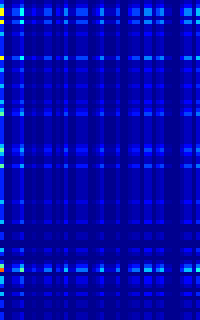
\includegraphics[width=0.25\textwidth]{know-10} }}%
    \qquad
    \subfloat[50 new samples]{{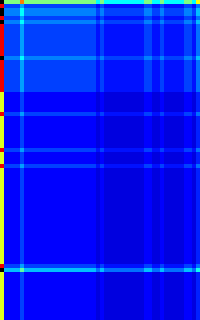
\includegraphics[width=0.25\textwidth]{know-50} }}%
    \qquad
    \subfloat[200 new samples]{{
\includegraphics[width=0.25\textwidth]{know-200} }}%
    
    Knowledge scaled is same as figure \ref{fig:min_know_search} - the darker the blue the less is known.
    \caption{Evolution of Knowledge Matrix over time}%
    \label{fig:know_mat_it}
\end{figure}

The main weakness in this algorithm is described in figure \ref{fig:know_mat_it}. As it targets the row-column combinations with the least knowledge the number of samples available for selection at each step can actually increase due to the matrix becoming more uniform. Thus the potential for sample discrimination decreases over time and the advantage only exists during initial matrix sampling. Initialising a search trial with many more known samples can cause minimum knowledge search to perform 20\% worse \footnote{In terms of advantage value}.

\subsection{Comments}
The minimum knowledge search algorithm does not take the known matrix elements, nor the predicted ones, into consideration. These also contain information in themselves and could greatly help with the selection of better samples. Being dataset agnostic is an weakness of minimum knowledge search as dataset properties can greatly impact performance. For example a dataset where a row and column that has most of the less useful elements known but very useful unknown elements will not be targeted until very late on, potentially giving the random sampling an edge. Minimum knowledge search only really works on datasets where useful elements are not found in clusters.

Additionally the aim of homogenising the amount known in each column and row is not always possible in constrained situations where the sampling space is limited, that is a sample determined for selection is not available(i.e. it may not be possible to ask a user his 5 star rating of a film if he hasn't seen it).

Algorithms presented later on will take advantage of the dataset to try and get better performance.

% ------------------------------------------------------------------------

%%% Local Variables: 
%%% mode: latex
%%% TeX-master: "../thesis"
%%% End: 

\chapter{Advanced Sample Selection}
\ifpdf
    \graphicspath{{Chapter3/Chapter3Figs/PNG/}{Chapter3/Chapter3Figs/PDF/}{Chapter3/Chapter3Figs/}}
\else
    \graphicspath{{Chapter3/Chapter3Figs/EPS/}{Chapter3/Chapter3Figs/}}
\fi


Now that we have a good idea of what active sampling involves attention will be focused to more advanced algorithms with the aim of improving performance.
\section{Clustered Knowledge Sampling}
\label{sec:cks}
\markboth{\MakeUppercase{\thechapter. Advanced Sample Selection }}{\thechapter. Advanced Sample Selection}
In the proposed minimum knowledge search algorithm (section \ref{sec:mks_alg}), its poor performance was mainly due to ignoring the data and only focusing on the mask matrix, which homogenised the amount of known samples. This had two problems, one in situations with search space constraints and the other for actually ignoring data and not taking "information" into account.


\subsection{Outline}

\begin{figure}[!htbp]
  \begin{center}
    \resizebox{\textwidth}{!}{% This file was created by matlab2tikz v0.4.7 running on MATLAB 8.1.
% Copyright (c) 2008--2014, Nico Schlömer <nico.schloemer@gmail.com>
% All rights reserved.
% Minimal pgfplots version: 1.3
% 
% The latest updates can be retrieved from
%   http://www.mathworks.com/matlabcentral/fileexchange/22022-matlab2tikz
% where you can also make suggestions and rate matlab2tikz.
% 
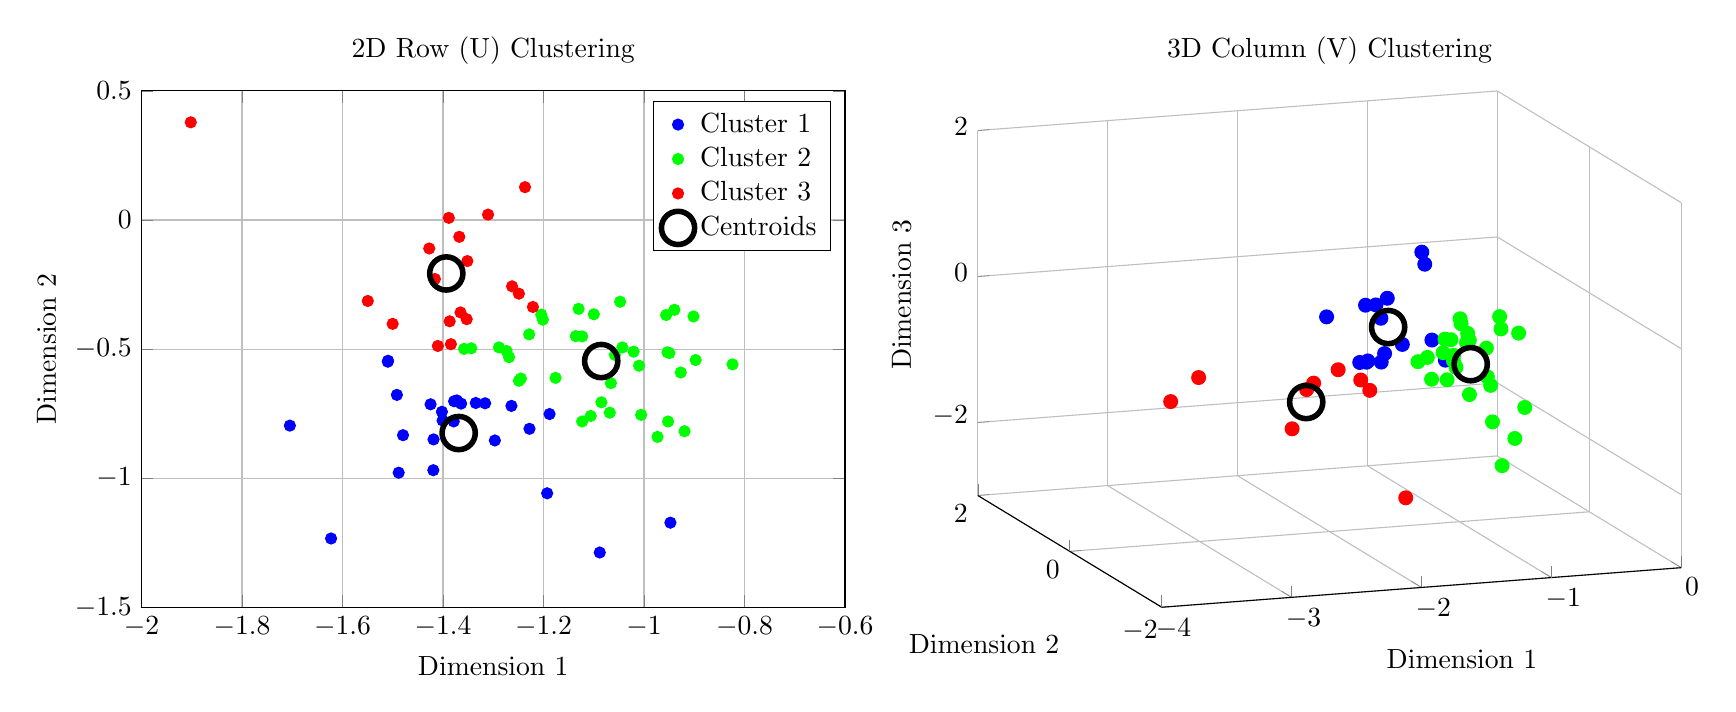
\begin{tikzpicture}

\begin{axis}[%
width=3.51740648674242in,
height=2.58151041666667in,
view={-19.5}{18},
scale only axis,
xmin=-4,
xmax=0,
xlabel={Dimension 1},
xmajorgrids,
ymin=-2,
ymax=2,
ylabel={Dimension 2},
ymajorgrids,
zmin=-3,
zmax=2,
zlabel={Dimension 3},
zmajorgrids,
name=plot1,
title={3D Column (V) Clustering},
axis x line*=bottom,
axis y line*=left,
axis z line*=left
]
\addplot3 [color=blue,mark size=2.5pt,only marks,mark=*,mark options={solid}]
 table[row sep=crcr] {-1.59044540063681	0.148396996168405	-0.00698558731390522\\
-1.86602726252353	-0.404299596558771	0.238047600835955\\
-2.15402023110266	-0.370963692226637	0.104703420377893\\
-2.01836370251589	-0.708482579480979	-0.409582767022601\\
-1.3601021205625	-0.263476524470756	0.677007101878209\\
-1.84863640992759	-0.405737385391855	-0.527296075866767\\
-1.8297149862398	-0.635270366202015	0.142259654037909\\
-1.85319119891177	-1.591979484085	1.4180250028355\\
-1.53407932701679	-1.2029284069621	-0.254406365200206\\
-1.96308377629313	-1.02005617297288	-0.292600342652495\\
-1.4800140593837	-0.757826699388731	-0.156283097895312\\
-1.98325658275392	-1.14987990275354	-0.123521101234678\\
-2.0902575666433	-1.06113716256017	-0.261223194073795\\
-1.6044250712648	-0.138809835184553	0.196026800172275\\
-1.79360406022386	-1.00024498034514	-0.0808198205638491\\
};
 \addplot3 [color=green,mark size=2.5pt,only marks,mark=*,mark options={solid}]
 table[row sep=crcr] {-1.47671051242454	-0.740544172774373	-0.700265880452768\\
-0.93252978607874	-0.737858573994506	-1.95864940281495\\
-1.39095127404548	-1.03082252266447	-0.436930323751058\\
-0.826190098315246	-0.796788433464611	-0.135195116811069\\
-1.14564673815213	-0.226979187418543	-0.400313692051324\\
-1.28640712006202	-0.454245485913808	-0.471703201832827\\
-1.07636956454563	-0.823100337923473	-0.689844042349405\\
-1.12469679933646	-0.389700844325155	-0.123064999816717\\
-1.09992565114399	-0.498384325340187	-0.31048726329556\\
-1.41309679459476	-1.38500223790909	-0.671990025552719\\
-1.25556262289311	-0.595096473274391	-0.458811626470363\\
-1.38017147536982	-0.806158272944827	-0.696454758506215\\
-1.1184806298713	-1.755123688963	-0.747224784979808\\
-1.0831580755134	-0.820895730212531	-0.296258382112644\\
-1.48188468231259	-0.460624191506098	-0.566309707097411\\
-1.11563748443596	-1.00507440936161	-0.732314861859024\\
-0.929163965552316	-0.519647699876556	-1.44361838242822\\
-1.19434558073037	-0.703961212433198	-0.251105760079353\\
-1.46380901634084	-0.611874379533737	-0.452599705977574\\
-1.31478254435664	-0.575143613118262	-0.236189435731263\\
-1.09688073201687	-0.289096106073911	-0.0960876831079487\\
-0.773050817612426	-0.233815087553789	-0.131884904110039\\
-0.813338320663528	-0.377167666478255	-0.24029048766129\\
-0.876771344375913	-0.857072651175691	-1.54870993973188\\
-1.14990983972071	-0.29358421798426	-0.663112219132381\\
-1.13003602840388	-0.546883342757847	-0.193711899583056\\
};
 \addplot3 [color=red,mark size=2.5pt,only marks,mark=*,mark options={solid}]
 table[row sep=crcr] {-2.11607881604296	-1.20309665474736	-0.589023084252537\\
-2.35807960849134	-1.19898464092221	-0.275036292209193\\
-2.45276407893644	-0.465205348869312	-1.35246640183301\\
-1.85926734892307	-1.25963112352855	-2.07438098640639\\
-3.47098887962986	-0.700065408270514	-0.751679331712361\\
-2.21876190776304	-1.29614469556361	-0.397752621498269\\
-2.47690496220663	-1.00083546374682	-0.518829309125334\\
-2.45427807746748	-0.78414820561212	-0.692778019848313\\
-3.4342351998618	-1.2039455085677	-0.234307040855988\\
};
 \addplot3 [color=black,line width=2.0pt,mark size=6.0pt,only marks,mark=o,mark options={solid}]
 table[row sep=crcr] {-1.79794811706667	-0.704179719494315	0.0442234152209426\\
-1.15190413457187	-0.674409417883699	-0.563581864896033\\
-2.53792876436918	-1.01245078331424	-0.765139231971266\\
};
 \end{axis}

\begin{axis}[%
width=3.51740648674242in,
height=2.58151041666667in,
scale only axis,
xmin=-2,
xmax=-0.6,
xlabel={Dimension 1},
xmajorgrids,
ymin=-1.5,
ymax=0.5,
ylabel={Dimension 2},
ymajorgrids,
at=(plot1.left of south west),
anchor=right of south east,
title={2D Row (U) Clustering},
legend style={draw=black,fill=white,legend cell align=left}
]
\addplot [color=blue,mark size=2.0pt,only marks,mark=*,mark options={solid}]
  table[row sep=crcr]{-0.947397094097976	-1.17240232446132\\
-1.42464042756946	-0.713815591075102\\
-1.22781208226467	-0.808765943560055\\
-1.37238484821147	-0.698803283515191\\
-1.37781059027466	-0.702054360358239\\
-1.08796797285841	-1.28792997752542\\
-1.41920362072619	-0.969141960295007\\
-1.49169444482093	-0.67739390245747\\
-1.26374363723324	-0.720049936258417\\
-1.33466016547064	-0.708718593754529\\
-1.48811954757637	-0.9788217818583\\
-1.1878838257152	-0.751578697212706\\
-1.36389755394777	-0.711223029487005\\
-1.50926630817321	-0.545099702809181\\
-1.40069149027704	-0.776586360666373\\
-1.50975621361547	-0.548801346804066\\
-1.37855408387926	-0.780159670397303\\
-1.31611978200492	-0.709930659849702\\
-1.418751280377	-0.849795612755271\\
-1.19267570375899	-1.05856633692692\\
-1.47951050417601	-0.833441522749927\\
-1.40210224009503	-0.742883948823392\\
-1.70466946988011	-0.796421429139088\\
-1.62266369930196	-1.23367702017733\\
-1.29673298795604	-0.853960506960763\\
};
\addlegendentry{Cluster 1};

\addplot [color=green,only marks,mark=*,mark options={solid}]
  table[row sep=crcr]{-0.952004639322655	-0.780407744162834\\
-1.35800804056431	-0.499095126768185\\
-1.12301132961619	-0.450813783470718\\
-1.06803088855719	-0.746252586925583\\
-1.04742072820829	-0.316512594208732\\
-1.00563006266044	-0.754667394539394\\
-1.08471290104999	-0.706052703408371\\
-0.972986130578649	-0.840038953765678\\
-0.926768452677666	-0.590670764290693\\
-1.10598706869137	-0.759020761417815\\
-1.12299454549838	-0.780455778963848\\
-1.34375616408669	-0.496931240615796\\
-0.823701319540284	-0.55922528432968\\
-1.27345811398	-0.506983755622736\\
-1.05784721496967	-0.52241729560441\\
-0.949405224340586	-0.515403391466322\\
-1.00973566569467	-0.564270108492813\\
-0.897178142840313	-0.542394334642152\\
-1.28850500158151	-0.493491662522362\\
-1.20120133077088	-0.385865901893781\\
-1.13005221396697	-0.344149415912444\\
-1.22851393427091	-0.442937560581115\\
-1.26844999472948	-0.531171960691112\\
-1.09980175514811	-0.365281432703934\\
-0.901446106339055	-0.373594412602389\\
-1.24886587648314	-0.622710283455377\\
-0.955827125951069	-0.368068581593385\\
-0.919233297957232	-0.818242177080642\\
-1.02058986705701	-0.509959799649133\\
-1.20447547808101	-0.36632574209671\\
-0.939403310754379	-0.347838228723723\\
-1.06577253942638	-0.631933383632939\\
-1.13563758881092	-0.449750374425283\\
-1.17592385721954	-0.611327813248462\\
-0.953229779684915	-0.512455651100702\\
-1.04297625053534	-0.493442994365538\\
-1.24488239946148	-0.61392004639489\\
};
\addlegendentry{Cluster 2};

\addplot [color=red,only marks,mark=*,mark options={solid}]
  table[row sep=crcr]{-1.38667570143095	-0.392327756779921\\
-1.90191402108737	0.37843174742415\\
-1.35145177681762	-0.159014906937421\\
-1.38834556565347	0.00828026112936182\\
-1.42731217565679	-0.110223842769362\\
-1.50012813166991	-0.402262676901485\\
-1.23673403705109	0.127286862615916\\
-1.54961317850779	-0.313606751908253\\
-1.38424609474405	-0.480950419640141\\
-1.41015507760762	-0.487840276904245\\
-1.31029966299755	0.0210377007725251\\
-1.3650626694132	-0.358014675162437\\
-1.35275033416153	-0.384139741274205\\
-1.24893755013947	-0.285353484220869\\
-1.22099935349909	-0.336870067395305\\
-1.36748608818927	-0.0650839050816374\\
-1.41608032676241	-0.228524593438377\\
-1.26244189537061	-0.256869879155967\\
};
\addlegendentry{Cluster 3};

\addplot [color=black,line width=2.0pt,mark size=6.0pt,only marks,mark=o,mark options={solid}]
  table[row sep=crcr]{-1.36874838297048	-0.825200939995123\\
-1.08506552273261	-0.54632651419918\\
-1.39336853559777	-0.207002578090426\\
};
\addlegendentry{Centroids};

\end{axis}
\end{tikzpicture}%}
  \end{center}
    
$U$ and $V$ from synthetic dataset with 15\% of samples initially discovered.  $\lambda = 0.01$, $D=7$

Dimensions reduced for plotting purposes
    \caption{Sample k-means clustering of U and V by features}
    \label{fig:u_v_cluster}
\end{figure}

Minimum knowledge search failed to integrate information about the known data to target more informative samples. Here we decide to take advantage of the $U$ and $V$ matrices formed during matrix factorisation, as in equation \ref{eq:rsimeq}. Each of the columns of $U$ and $V$ are supposed to represent features of the related row or column. We now assume that if we knew a minimal amount of each feature it will be possible to cluster rows and columns into groups. Figure \ref{fig:u_v_cluster} shows the features of U and V clustered into 3 different groups\footnote{3 was arbitrarily chosen as the number of clusters}. In the case of drug-target interaction database dimension 1 could represent the estimated presence of a chemical, say $H_2O$ and the second dimension of the presence that represents the presence of another chemical.

In collaborative filtering we seek to infer these features to best reconstruct the full matrix. The idea behind clustered sample selection is to target the groups with the least certainty, to improve their accuracy and the model as a whole. In a movie-user scenario this means that we can separate the thriller film liking users from the drama movie liking users, then if we find out that less is know on thriller liking people then the model should be better off learning an extra datapoint on that group. This would allow for row selection and the selection of columns can be done in a similar way. We will define knowledge in the same way as minimum knowledge search, as the fraction of known rows and columns.



\subsection{Algorithm}

We base the work of the clustered knowledge search on the minimum knowledge search algorithm, in that we will target not the specfic row-column combination we know less about but the row-colum cluster we know the less about. 

The first step involves determining the ideal number of clusters for a dataset. In itself this is not an easy task and can increase algorithm complexity due to having to test for all different candidate number of clusters. To determine the number of clusters we use the silhouette measure \cite{kmean-sil} which essentially measures how tight data is when in a group. It is not always effective but does the job. 
%Explain how to cluster in silhoutettes



\begin{algorithm}
\caption{Clustered Knowledge Search algorithm}\label{alg:cks}
\begin{algorithmic}[1]
\Procedure{ClusKnowSearch}{$U$,$V$,$Z$}
\State $k_U \gets \text{NumOfClust}(U)$ \Comment{Returns best guess of number of clusters}
\State $k_V \gets \text{NumOfClust}(V)$
\State $u_{\text{clusters}} = \text{kmeans}(U,k_U)$ \Comment{Assigns cluster IDs}
\State $v_{\text{clusters}} = \text{kmeans}(V,k_V)$
\State $\mathbf{u_{info}} \gets \text{meanrow}(Z)$ \Comment{$\in \mathbb{R}^N$}
\State $\mathbf{v_{info}} \gets \text{meancol}(Z)$ \Comment{$\in \mathbb{R}^M$}
\State $\mathbf{a} \gets \mathbf{0}^{N}$ \Comment{$\in \mathbb{R}^N$}
\State $\mathbf{b} \gets \mathbf{0}^{M}$ \Comment{$\in \mathbb{R}^M$}
\For{$i=1\dots k_U$}
\State $\mathbf{u_{knowl}}[i] \gets \sum\limits_{\text{index}=i} \mathbf{u_{info}}$ \Comment{Adds up all info values}
\State $\mathbf{a}[{index\; u_{\text{clusters}} =i}] = \mathbf{u_{knowl}}[i]$ \Comment{Assigns sum of info to clusters}
\EndFor

\For{$j=1\dots k_V$}
\State $\mathbf{v_{knowl}}[j] \gets \sum\limits_{\text{index}=j} \mathbf{v_{info}}$
\State $\mathbf{b}[{index\; v_{\text{clusters}} =j}] = \mathbf{v_{knowl}}[j]$
\EndFor

\State $K \gets \mathbf{a}^T \cdot \mathbf{b}$ \Comment{ $K \in \mathbb{R}^{M\times N}$}
\State $x,y \gets index\_of\_min(K)$ \Comment{Many candidates, one is chosen at random} \label{alg:line:select}
\While{$x,y$ not valid sample request}
\State $x,y \gets next\_min\_index(K)$
\EndWhile
\State \textbf{return} $x,y$\Comment{Return $x,y$ that has least knowledge}
\EndProcedure
\end{algorithmic}
\end{algorithm}

Once we have determined the number of clusters, we cluster the rows and columns according to the features of $U$ and $V$ using a clustering algorithm. K-means was chosen for being fast yet good at clustering. Alternatives such as GMM were considered but found to not be appropriate due to their great increase in complexity and little increase in clustering quality - further work could look into better clustering algorithm.

\nomenclature{GMM}{Gaussian Mixture Model - A probabilistic model for representing the presence of subsets within an overall dataset}

\nomenclature{K-Means}{K-Means Clustering - A popular algorithm for cluster analysis, which separates $N$ data points into $K$ clusters around centroids}


From the clustered rows we create the vectors $\mathbf{a}$ and $\mathbf{b}$ which contain the amount know of each cluster. This allows the create of the knowledge matrix, $K =\mathbf{a}^T \cdot \mathbf{b}$. From this a sample is selected as in section \ref{sec:mks_alg}.

This algorithm is defined formally in algorithm \ref{alg:cks}.
%\subsubsection{Clustering observations}
%... and some more in the first subsub section otherwise it all looks the same
%doesn't it? well we can add some text to it ...

\subsection{Performance}
The first initial observations on the performance is that during a cold-start, that is when very little is know about the matrix, clustering will not perform well and sample selection will effectively be random. As soon as enough data is gathered a large advantage compared to random sampling is usually observed. This is because, unlike the minimum knowledge search, the search area is always restricted to a reasonably small subset.


It will also tend to cluster currently unknown groups of data together and targeting them even later on in execution which is useful. However once the number of unknown rows and columns have fallen down it suffers from not requesting individual rows and columns with no knowledge if they are assigned to a cluster of high information - this seemed to be the main drawback from this algorithm. This can be seen from the lines in figure \ref{fig:eiffel_clustering_random} which are never requested. This is why it is preferred to randomly sample from the restricted subset (line \ref{alg:line:select} in algorithm \ref{alg:cks}) as it can mitigate this problem. In cases where the first available value of the subset is selected, the algorithm was found to sometimes perform worse than random in very late stages, due to removing the ability to sample from certain, useful, areas.



\begin{figure}[!htbp]
  \begin{center}
    \resizebox{\textwidth}{!}{% This file was created by matlab2tikz v0.4.7 running on MATLAB 8.1.
% Copyright (c) 2008--2014, Nico Schlömer <nico.schloemer@gmail.com>
% All rights reserved.
% Minimal pgfplots version: 1.3
% 
% The latest updates can be retrieved from
%   http://www.mathworks.com/matlabcentral/fileexchange/22022-matlab2tikz
% where you can also make suggestions and rate matlab2tikz.
% 
\begin{tikzpicture}

\begin{axis}[%
width=1.67990913120567in,
height=2.06885416666667in,
axis on top,
scale only axis,
xmin=0.5,
xmax=50.5,
y dir=reverse,
ymin=0.5,
ymax=80.5,
name=plot2,
title={Targeted RMSE:0.806}
]
\addplot [forget plot] graphics [xmin=0.5,xmax=50.5,ymin=0.5,ymax=80.5] {eiffel_clustering_random-1.png};
\end{axis}

\begin{axis}[%
width=1.67990913120567in,
height=2.06885416666667in,
axis on top,
scale only axis,
xmin=0.5,
xmax=50.5,
y dir=reverse,
ymin=0.5,
ymax=80.5,
at=(plot2.left of south west),
anchor=right of south east,
title={Random RMSE:0.839}
]
\addplot [forget plot] graphics [xmin=0.5,xmax=50.5,ymin=0.5,ymax=80.5] {eiffel_clustering_random-2.png};
\end{axis}

\begin{axis}[%
width=1.67990913120567in,
height=2.06885416666667in,
scale only axis,
xmin=0,
xmax=1000,
xlabel={Discovered Samples},
xmajorgrids,
ymin=0.5,
ymax=3.5,
ylabel={RMSE},
ymajorgrids,
name=plot3,
at=(plot2.right of south east),
anchor=left of south west,
title={Target Advantage:1.033}
]
\addplot [color=blue,solid,forget plot]
  table[row sep=crcr]{1	3.23608821969601\\
4	3.23874456682935\\
7	3.23400303366272\\
10	3.22686273151906\\
13	3.22064145645356\\
16	3.210065518808\\
19	3.20609812591828\\
22	3.20094180016412\\
25	3.19290280170711\\
28	3.18218381413051\\
31	3.16964031933361\\
34	3.1683939149483\\
37	3.14902695809985\\
40	3.14063222906248\\
43	3.13273566512044\\
46	3.13792693466917\\
49	3.13819075795978\\
52	3.13919418631302\\
55	3.12774596457256\\
58	3.10462488420985\\
61	3.08908746474799\\
64	3.06099903675343\\
67	3.03884916723113\\
70	2.99517372420138\\
73	2.97196825627754\\
76	2.97256611010417\\
79	2.95382968686519\\
82	2.95634785166779\\
85	2.94868953281047\\
88	2.94325789737375\\
91	2.94350848161074\\
94	2.91336774342895\\
97	2.90056982311092\\
100	2.85923501691438\\
103	2.83740090301335\\
106	2.79845083538125\\
109	2.77376523447295\\
112	2.75413976151122\\
115	2.74400949224298\\
118	2.70028004286642\\
121	2.67358627982908\\
124	2.62618230680027\\
127	2.5991518051474\\
130	2.56216884913842\\
133	2.50799167659206\\
136	2.50385337795266\\
139	2.4803382802154\\
142	2.44636183251382\\
145	2.41592726658385\\
148	2.39933224583661\\
151	2.40277511320256\\
154	2.34731779980291\\
157	2.3070855826964\\
160	2.2896257555724\\
163	2.23026298414911\\
166	2.21708749193983\\
169	2.17344338947626\\
172	2.13681549115793\\
175	2.13195859805556\\
178	2.08980570866445\\
181	2.07051216580413\\
184	2.0290780770062\\
187	2.00290502932381\\
190	1.97208451698914\\
193	1.94062234122199\\
196	1.91740161345952\\
199	1.87986542638094\\
202	1.84671693422685\\
205	1.82186129157887\\
208	1.79450537588702\\
211	1.76763352842766\\
214	1.74168676243316\\
217	1.72430216808774\\
220	1.71889477376259\\
223	1.68961112331644\\
226	1.67025781087249\\
229	1.65326196179016\\
232	1.60945972087621\\
235	1.58258047471896\\
238	1.54487313115169\\
241	1.51817513386755\\
244	1.49070521269874\\
247	1.46080281702285\\
250	1.44720905111535\\
253	1.43926025170762\\
256	1.40292904023112\\
259	1.38659439540347\\
262	1.37895909165236\\
265	1.35672297317994\\
268	1.35092785676313\\
271	1.33117400480906\\
274	1.33258414460804\\
277	1.3253190477257\\
280	1.31368167800342\\
283	1.29119318682901\\
286	1.2847957937692\\
289	1.26668265767296\\
292	1.24925263988163\\
295	1.22933860498004\\
298	1.22269200109639\\
301	1.217588049285\\
304	1.20608664660767\\
307	1.19807300208598\\
310	1.19758312124881\\
313	1.1938256302761\\
316	1.18716489873387\\
319	1.19029671808817\\
322	1.18292779724569\\
325	1.17282069844146\\
328	1.15851505986828\\
331	1.15456764680907\\
334	1.14508764016097\\
337	1.12668385447176\\
340	1.11143941981602\\
343	1.10514593946996\\
346	1.10304784064215\\
349	1.10116816111664\\
352	1.09107633565513\\
355	1.08633596051687\\
358	1.08516499819841\\
361	1.07959210657411\\
364	1.07530032022216\\
367	1.07216539510789\\
370	1.06622687994884\\
373	1.06630297628754\\
376	1.06260705350293\\
379	1.06175827182202\\
382	1.06143183296372\\
385	1.05791649140148\\
388	1.05409250877161\\
391	1.05161336131875\\
394	1.05116623420654\\
397	1.05016516103723\\
400	1.04877986780112\\
403	1.04630129440592\\
406	1.04418511076514\\
409	1.04450441148256\\
412	1.0411350617253\\
415	1.04074781344838\\
418	1.04105816040508\\
421	1.03891783350241\\
424	1.03846898033468\\
427	1.03366056108131\\
430	1.0349054643268\\
433	1.03293572208455\\
436	1.02914529258533\\
439	1.02837604894394\\
442	1.02288217203224\\
445	1.01917734623858\\
448	1.01660529190564\\
451	1.01104633503953\\
454	1.00738780460553\\
457	1.00472484329262\\
460	1.0039520994342\\
463	1.00523368157343\\
466	1.0034014855957\\
469	1.00115415201671\\
472	1.00131717115537\\
475	1.00140154452006\\
478	0.999600501577712\\
481	0.997030854659885\\
484	0.996596829338407\\
487	0.998956506591063\\
490	0.996396119941576\\
493	0.99678747484711\\
496	0.995812517884907\\
499	0.996549742510299\\
502	0.997814025890126\\
505	0.997465160219533\\
508	0.998205183905975\\
511	0.996700572212048\\
514	0.992192014135254\\
517	0.99017274589718\\
520	0.988246220181901\\
523	0.983527543116826\\
526	0.980158352527665\\
529	0.976936631596359\\
532	0.973841590288914\\
535	0.971683759345203\\
538	0.97021998537905\\
541	0.970087303017605\\
544	0.966875404562843\\
547	0.965446355399993\\
550	0.961156860324029\\
553	0.960736860199741\\
556	0.959573196397698\\
559	0.958172455028803\\
562	0.958770783614183\\
565	0.95942333309407\\
568	0.95675523315015\\
571	0.954985652638341\\
574	0.953754982262894\\
577	0.951951640394101\\
580	0.950033484240326\\
583	0.947777327611643\\
586	0.944826363270912\\
589	0.944952886290964\\
592	0.94315558643634\\
595	0.941699990458453\\
598	0.938536696327822\\
601	0.937049163550473\\
604	0.936679555970613\\
607	0.936292576650164\\
610	0.934670013600377\\
613	0.933201096489967\\
616	0.932154862665519\\
619	0.935070401434189\\
622	0.935818514423071\\
625	0.934527979357141\\
628	0.934906714264051\\
631	0.935615129794311\\
634	0.936366242579699\\
637	0.935284780247618\\
640	0.932280549739419\\
643	0.931216722723593\\
646	0.930150141619051\\
649	0.928546240457424\\
652	0.925445991397538\\
655	0.92497766091949\\
658	0.92524494521337\\
661	0.925938557632788\\
664	0.921872445167552\\
667	0.922655597972024\\
670	0.926914387150573\\
673	0.923358707406725\\
676	0.918656594203506\\
679	0.923113626000366\\
682	0.923673712709766\\
685	0.923765488220372\\
688	0.925829658005833\\
691	0.928196910759219\\
694	0.930349324771632\\
697	0.930915786574827\\
700	0.928988500185951\\
703	0.931445992770396\\
706	0.931045664349461\\
709	0.930085759627698\\
712	0.927684194495509\\
715	0.924206707903442\\
718	0.917216929973831\\
721	0.9138815695211\\
724	0.910281899990097\\
727	0.9048235024033\\
730	0.901690576891687\\
733	0.901556019448105\\
736	0.901076836371851\\
739	0.898997400601895\\
742	0.898609734264734\\
745	0.898487285087361\\
748	0.896874150045249\\
751	0.896184674262905\\
754	0.89464558708581\\
757	0.89371816401248\\
760	0.891675939489928\\
763	0.889270954104735\\
766	0.887393356920999\\
769	0.888966477789644\\
772	0.889796743924115\\
775	0.889217325274594\\
778	0.886175970567902\\
781	0.887831673635639\\
784	0.884393887310554\\
787	0.881405784230714\\
790	0.875125770607302\\
793	0.875491739240181\\
796	0.873320815865276\\
799	0.872607897223783\\
802	0.871275216169282\\
805	0.870729415201652\\
808	0.868897845035715\\
811	0.867814864589322\\
814	0.865641713524941\\
817	0.867104401643685\\
820	0.864460449379786\\
823	0.865104730667196\\
826	0.864160878179792\\
829	0.864625887542073\\
832	0.863328213106487\\
835	0.860767751860216\\
838	0.859966998307642\\
841	0.857019519810177\\
844	0.857987718098942\\
847	0.856739782088524\\
850	0.856577326039197\\
853	0.856560098757885\\
856	0.854184426682648\\
859	0.85348915660362\\
862	0.851685450224478\\
865	0.848851766170523\\
868	0.849928253030711\\
871	0.851961364717722\\
874	0.853659193033011\\
877	0.856835734709883\\
880	0.859220693886935\\
883	0.863043394077267\\
886	0.865315484430734\\
889	0.866086515663051\\
892	0.867300737937679\\
895	0.868230565044493\\
898	0.868322860414097\\
901	0.86568408442662\\
904	0.861998055926054\\
907	0.86052347090935\\
910	0.859925430757205\\
913	0.858086205182545\\
916	0.857451962604108\\
919	0.856321452316256\\
922	0.858089207726632\\
925	0.856844921576297\\
928	0.853638586216406\\
931	0.85396213461611\\
934	0.852728595458033\\
937	0.851397625110357\\
940	0.852107411623177\\
943	0.852585438816453\\
946	0.853087631098825\\
949	0.853034693501791\\
952	0.851691813071311\\
955	0.850075931017224\\
958	0.849901912244008\\
961	0.85075354738233\\
964	0.850944767696275\\
967	0.852958404901457\\
970	0.852455885899463\\
973	0.853813692669622\\
976	0.850166490037983\\
979	0.842975103185344\\
982	0.83575002197476\\
985	0.827782779485582\\
988	0.820562807360585\\
991	0.81380117214787\\
994	0.808463151894714\\
997	0.807083983661091\\
1000	0.805551012207653\\
};
\addplot [color=black!50!green,solid,forget plot]
  table[row sep=crcr]{1	3.24667882730123\\
4	3.2435760427341\\
7	3.2438488616279\\
10	3.2424788351965\\
13	3.24088412783809\\
16	3.23948781631039\\
19	3.23556651206499\\
22	3.23217273672512\\
25	3.2300815993755\\
28	3.23065844219907\\
31	3.22997790456822\\
34	3.2270553385783\\
37	3.22116850178826\\
40	3.21877709340252\\
43	3.20660229985026\\
46	3.19044056467919\\
49	3.18148218093542\\
52	3.17677886402666\\
55	3.17964492085272\\
58	3.14798984955541\\
61	3.14866997577402\\
64	3.14199420790457\\
67	3.14922638803591\\
70	3.13272093075182\\
73	3.1041246960365\\
76	3.09495763692531\\
79	3.05083523201981\\
82	3.05979709428272\\
85	3.02802925777727\\
88	3.02621565795659\\
91	3.01363816272817\\
94	2.97206618284224\\
97	2.96627103645061\\
100	2.88848078228225\\
103	2.90892165749103\\
106	2.89217936301548\\
109	2.91002875512088\\
112	2.84100163670117\\
115	2.77656105100302\\
118	2.72226625688616\\
121	2.64718886956543\\
124	2.57230614466224\\
127	2.51796311084138\\
130	2.51341345162893\\
133	2.457934677154\\
136	2.41216464329626\\
139	2.39019724926956\\
142	2.41979527654761\\
145	2.42997988194484\\
148	2.36767403079863\\
151	2.34220014133621\\
154	2.27146555058509\\
157	2.26381175648033\\
160	2.19015834157452\\
163	2.17901333427551\\
166	2.12729776359819\\
169	2.14037190936422\\
172	2.11685132555664\\
175	2.10032067546914\\
178	2.04802767273072\\
181	2.01009719871541\\
184	1.96507594315842\\
187	1.95127289197761\\
190	1.92107992050017\\
193	1.94255439202863\\
196	1.92109968419691\\
199	1.90327933898412\\
202	1.87919365605718\\
205	1.86622355233829\\
208	1.81965592005564\\
211	1.7868256534388\\
214	1.72202671957349\\
217	1.68833205456928\\
220	1.66841794704626\\
223	1.61679766966419\\
226	1.58070358282027\\
229	1.52129843610789\\
232	1.50601491932452\\
235	1.4882803549476\\
238	1.48374290333434\\
241	1.48014628253269\\
244	1.47116790096055\\
247	1.4689533454162\\
250	1.45729960830311\\
253	1.44961088872314\\
256	1.42798386598537\\
259	1.40611829124032\\
262	1.38007571775529\\
265	1.35823667444576\\
268	1.34478238699759\\
271	1.35743427365165\\
274	1.34523611019655\\
277	1.34574532570706\\
280	1.33118640223234\\
283	1.32423683908421\\
286	1.34537145116777\\
289	1.32494914943826\\
292	1.31807964605098\\
295	1.30459315471877\\
298	1.30517504765669\\
301	1.28921748440169\\
304	1.26520659366356\\
307	1.25925431390801\\
310	1.25714531537487\\
313	1.26200670498607\\
316	1.26754791348723\\
319	1.25632331458006\\
322	1.24209484897227\\
325	1.24977467352911\\
328	1.26843905604531\\
331	1.26418479880575\\
334	1.22786010557008\\
337	1.19409108238437\\
340	1.177937734003\\
343	1.16186774532945\\
346	1.16082118933295\\
349	1.15215819838023\\
352	1.1655364185071\\
355	1.17096808333259\\
358	1.16916767693502\\
361	1.16399921373453\\
364	1.1613093140485\\
367	1.16450511690737\\
370	1.16631905601109\\
373	1.17232111936959\\
376	1.16521640201083\\
379	1.15713648874277\\
382	1.14680368798413\\
385	1.14920238366715\\
388	1.139541614917\\
391	1.14287924400412\\
394	1.1380485365836\\
397	1.14424166003219\\
400	1.13991841915678\\
403	1.15366396822683\\
406	1.15071835619347\\
409	1.14236702688225\\
412	1.13279698582236\\
415	1.13770432805869\\
418	1.13296652412981\\
421	1.1180821456956\\
424	1.10585566982699\\
427	1.10133012732575\\
430	1.10225968583522\\
433	1.10341975436429\\
436	1.11024641731785\\
439	1.11037555971131\\
442	1.10705606366527\\
445	1.09610234736523\\
448	1.0950737935554\\
451	1.09792403272501\\
454	1.09880450602705\\
457	1.09654946250601\\
460	1.09795586229571\\
463	1.0922687520895\\
466	1.09731976262045\\
469	1.08960784530391\\
472	1.09175052829022\\
475	1.08706236574414\\
478	1.08514859063252\\
481	1.0822850318279\\
484	1.07444778644049\\
487	1.07526638679887\\
490	1.07660283066706\\
493	1.06687601079684\\
496	1.06424549530261\\
499	1.0572345901834\\
502	1.06675235376528\\
505	1.06183273149632\\
508	1.06048086233928\\
511	1.06126709229488\\
514	1.05932795141337\\
517	1.05388946366008\\
520	1.04486940768727\\
523	1.03999931790233\\
526	1.04148493214252\\
529	1.04546496169882\\
532	1.04134978253229\\
535	1.04440914511982\\
538	1.03658985214061\\
541	1.03143140969346\\
544	1.02502617798373\\
547	1.01774513854361\\
550	1.01874344246358\\
553	1.01348062013771\\
556	1.01674044903832\\
559	1.01803559855934\\
562	1.01336516833175\\
565	1.01078502040422\\
568	1.00592116880043\\
571	1.00318651428343\\
574	1.00752120419032\\
577	1.00437341140392\\
580	1.01058269364257\\
583	1.00221116715667\\
586	1.00238413439302\\
589	0.99476630198291\\
592	0.993451005967499\\
595	0.987198605014026\\
598	0.983157931766563\\
601	0.979326347997727\\
604	0.98083913781656\\
607	0.988361597463705\\
610	0.992518985657409\\
613	0.994260917003344\\
616	0.990682237329702\\
619	0.987508636894006\\
622	0.983797828412314\\
625	0.97878209008954\\
628	0.969252406005422\\
631	0.96688715935815\\
634	0.965365010557941\\
637	0.965191067105658\\
640	0.963171900774426\\
643	0.956248304078486\\
646	0.954346031893998\\
649	0.950033740246131\\
652	0.952186971157129\\
655	0.945831452647525\\
658	0.948742300482949\\
661	0.950006299853029\\
664	0.956173826494509\\
667	0.955494373423616\\
670	0.953162007175834\\
673	0.950442366455411\\
676	0.946215130001838\\
679	0.947135405501538\\
682	0.948271153818378\\
685	0.949460308418332\\
688	0.9494097006112\\
691	0.952873220507865\\
694	0.951047059786972\\
697	0.948452598239001\\
700	0.947865478083654\\
703	0.949565265032962\\
706	0.949128157443452\\
709	0.943419051639621\\
712	0.940662065513259\\
715	0.940538490546073\\
718	0.940010658657872\\
721	0.936309123390409\\
724	0.929518963498868\\
727	0.924689271759408\\
730	0.925187302000752\\
733	0.932043152159921\\
736	0.932747386666725\\
739	0.932485061603865\\
742	0.928094539357111\\
745	0.927988427374509\\
748	0.924485248939693\\
751	0.92116173876263\\
754	0.916546132969657\\
757	0.921944326255094\\
760	0.920764965446072\\
763	0.921585179482203\\
766	0.920346831536161\\
769	0.920842207079354\\
772	0.92525630135009\\
775	0.91874041549047\\
778	0.915766251418009\\
781	0.909089712905178\\
784	0.910501802901478\\
787	0.905088554209274\\
790	0.900185329061209\\
793	0.894228546373429\\
796	0.89811679165602\\
799	0.90240975028097\\
802	0.903339053536558\\
805	0.900977365569723\\
808	0.895406648502211\\
811	0.886991564576314\\
814	0.883384272083953\\
817	0.879795840693289\\
820	0.877232423590057\\
823	0.87283118249419\\
826	0.874154384837074\\
829	0.877027421211353\\
832	0.878591959259125\\
835	0.874612174887775\\
838	0.872100121645488\\
841	0.870674442796846\\
844	0.874327334458882\\
847	0.880808384055368\\
850	0.875020334631098\\
853	0.872576255696658\\
856	0.866689228335173\\
859	0.867178084061787\\
862	0.861890947661884\\
865	0.85674550969247\\
868	0.857512919078819\\
871	0.855531390089869\\
874	0.851569743302146\\
877	0.847040212364781\\
880	0.847618130202726\\
883	0.852294329606801\\
886	0.857095354071123\\
889	0.858816453136022\\
892	0.860393032276869\\
895	0.85922670095144\\
898	0.858123540641051\\
901	0.854468354982509\\
904	0.851935702195683\\
907	0.850413727403093\\
910	0.854125825451894\\
913	0.855001250485642\\
916	0.854270294889417\\
919	0.850223890352724\\
922	0.850124052901973\\
925	0.8540631442743\\
928	0.852204277011117\\
931	0.844677105499305\\
934	0.838682820864548\\
937	0.836156918492309\\
940	0.839602997937953\\
943	0.83664986483535\\
946	0.839087398595206\\
949	0.842110730998713\\
952	0.848585252548505\\
955	0.846223207421055\\
958	0.8426674811306\\
961	0.837203358332947\\
964	0.835680003871634\\
967	0.83390118871131\\
970	0.830896259348348\\
973	0.832521354485093\\
976	0.832985621662204\\
979	0.833204284259533\\
982	0.830236193476539\\
985	0.832480992134418\\
988	0.833253546474358\\
991	0.837248620566774\\
994	0.833591124219517\\
997	0.833361915991257\\
1000	0.819160550168973\\
};
\end{axis}

\begin{axis}[%
width=1.67990913120567in,
height=2.06885416666667in,
axis on top,
scale only axis,
xmin=0.5,
xmax=50.5,
y dir=reverse,
ymin=0.5,
ymax=80.5,
at=(plot3.right of south east),
anchor=left of south west,
title={Targeted Samples Matrix}
]
\addplot [forget plot] graphics [xmin=0.5,xmax=50.5,ymin=0.5,ymax=80.5] {eiffel_clustering_random-3.png};
\end{axis}
\end{tikzpicture}%}
  \end{center}
    
5\% of samples initially discovered.  PMF $\lambda = 0.01$, $D=15$

 The targeted samples matrix uses the same scale as in figure \ref{fig:min_know_search}. The darker blue the colour is the earlier on it was targeted.
 
 Blue line is targeted sampling and green on is random sampling.
 
 
 The random subgroup sampling method was employed for algorithm \ref{alg:cks}
    \caption{Clustering Knowledge Search on Eiffel Tower Image}
    \label{fig:eiffel_clustering_random}
\end{figure}
%Not good at the very start nor at the very end
%very weakness in the clustering

In figure \ref{fig:eiffel_clustering_random} we see from the targeted samples matrix that the search first started a bit randomly (the scatter blue points) and that as data was gathered the areas with higher data variance were targeted, that is the groups belonging to level 1 and 2 of the Eiffel tower. A realtime simulation of allows us to see that the sky area of the picture is discovered early on and then ignored in favour of the more complex areas of the structure.


\begin{figure}[!htbp]
  \begin{center}
    \resizebox{\textwidth}{!}{% This file was created by matlab2tikz v0.4.7 running on MATLAB 8.1.
% Copyright (c) 2008--2014, Nico Schlömer <nico.schloemer@gmail.com>
% All rights reserved.
% Minimal pgfplots version: 1.3
% 
% The latest updates can be retrieved from
%   http://www.mathworks.com/matlabcentral/fileexchange/22022-matlab2tikz
% where you can also make suggestions and rate matlab2tikz.
% 
\begin{tikzpicture}

\begin{axis}[%
width=2.33197463768116in,
height=2.48604166666667in,
scale only axis,
xmin=0,
xmax=500,
xlabel={Discovered Samples},
xmajorgrids,
ymin=1,
ymax=2.4,
ylabel={RMSE},
ymajorgrids,
name=plot2,
title={Target Advantage:1.071},
legend style={draw=black,fill=white,legend cell align=left}
]
\addplot [color=blue,solid]
  table[row sep=crcr]{1	2.09605205419641\\
4	2.0855430113021\\
7	2.08215350992599\\
10	2.08076905420891\\
13	2.07262994903198\\
16	2.06524859322496\\
19	2.05717813146063\\
22	2.05337127630108\\
25	2.04116496679461\\
28	2.02981996005782\\
31	2.02155390879592\\
34	2.02085865449889\\
37	2.01303207615211\\
40	2.00665473454645\\
43	2.00317754669449\\
46	1.99435320801059\\
49	1.99659896706514\\
52	1.98912331303213\\
55	1.97659075819099\\
58	1.97792409993712\\
61	1.9695393608528\\
64	1.96528414491713\\
67	1.95429159654481\\
70	1.94494852518109\\
73	1.9464349293184\\
76	1.94273396242194\\
79	1.93167893276328\\
82	1.93068046862956\\
85	1.92522767931863\\
88	1.92158785710357\\
91	1.92117581757485\\
94	1.9041472552041\\
97	1.89907811254786\\
100	1.89109582552751\\
103	1.89387627790631\\
106	1.87949471479236\\
109	1.87341897838324\\
112	1.86975263700992\\
115	1.86003368056268\\
118	1.86554281169786\\
121	1.85470843092767\\
124	1.85102596897277\\
127	1.85160746794753\\
130	1.81928225214668\\
133	1.81366870390674\\
136	1.79366467140847\\
139	1.76475114490131\\
142	1.74532478994513\\
145	1.72472698172917\\
148	1.71841325854495\\
151	1.70057375679975\\
154	1.69504315183158\\
157	1.67092276901866\\
160	1.64912612625297\\
163	1.61379430409187\\
166	1.61283040265372\\
169	1.58798688741805\\
172	1.57429665159345\\
175	1.54562346671792\\
178	1.54353797870172\\
181	1.55725113439967\\
184	1.55676029375658\\
187	1.55597804873342\\
190	1.5523840127028\\
193	1.54504684678957\\
196	1.55380751358153\\
199	1.52989574628472\\
202	1.50795433116074\\
205	1.50395771803547\\
208	1.51603617658917\\
211	1.51044738011589\\
214	1.49526625199149\\
217	1.48802328699252\\
220	1.49610201516608\\
223	1.49587081983262\\
226	1.47313698768501\\
229	1.44223552218718\\
232	1.42314816114629\\
235	1.40082785627838\\
238	1.37518666595413\\
241	1.35958045033887\\
244	1.33165702248063\\
247	1.32460197629359\\
250	1.33105657465142\\
253	1.32049326466402\\
256	1.31366387223641\\
259	1.29949310460994\\
262	1.2938087646916\\
265	1.28652308710179\\
268	1.28143205205379\\
271	1.27099953481464\\
274	1.26339318206054\\
277	1.25922787108336\\
280	1.24850334230023\\
283	1.24673964569477\\
286	1.24879050855337\\
289	1.2454236347872\\
292	1.24536647461714\\
295	1.23593920840588\\
298	1.2277237229873\\
301	1.22707443027193\\
304	1.21450504876381\\
307	1.19224992690447\\
310	1.18077273327932\\
313	1.16854637393525\\
316	1.1626155906597\\
319	1.15223055993071\\
322	1.13961785778857\\
325	1.1337480229769\\
328	1.13445119187484\\
331	1.13238355864625\\
334	1.1279113196251\\
337	1.12915992208297\\
340	1.12441111624259\\
343	1.11749351587456\\
346	1.11542123548305\\
349	1.10875901057834\\
352	1.10836781551794\\
355	1.10556501099893\\
358	1.10160905045129\\
361	1.0973748371512\\
364	1.0994444725723\\
367	1.10590147735777\\
370	1.10354880217436\\
373	1.09906555445215\\
376	1.10097281108099\\
379	1.09843607500988\\
382	1.09106965919488\\
385	1.08364654253632\\
388	1.08301589099838\\
391	1.08251017515203\\
394	1.07799246950119\\
397	1.07479903172157\\
400	1.074007479146\\
403	1.07201018790714\\
406	1.07008138251254\\
409	1.06568161522971\\
412	1.06185274162314\\
415	1.06141919191099\\
418	1.06015925293404\\
421	1.05834543697727\\
424	1.05410028248408\\
427	1.0541162791023\\
430	1.05342990451194\\
433	1.04885552437551\\
436	1.0444778200324\\
439	1.04328452887219\\
442	1.03959619564161\\
445	1.03589843569877\\
448	1.03088253205482\\
451	1.02808842696167\\
454	1.02642837689159\\
457	1.02348591620633\\
460	1.02106017570418\\
463	1.02091226569726\\
466	1.02007539210071\\
469	1.02294943041959\\
472	1.0240879856085\\
475	1.02223793867073\\
478	1.02028351454013\\
481	1.01911875718392\\
484	1.01704224749965\\
487	1.01552532552276\\
490	1.01458873980993\\
493	1.01490317939285\\
496	1.01605756568797\\
499	1.02176603559748\\
500	1.0219646592255\\
};
\addlegendentry{Targeted sampling};

\addplot [color=black!50!green,solid]
  table[row sep=crcr]{1	2.08737177550677\\
4	2.08467184403021\\
7	2.08298650087891\\
10	2.08348084945761\\
13	2.08235832565932\\
16	2.08278336567022\\
19	2.07997182596675\\
22	2.07911563225928\\
25	2.07822621974444\\
28	2.07619799809029\\
31	2.07509690461574\\
34	2.07037368540558\\
37	2.06796467565784\\
40	2.06249287777274\\
43	2.06005976089149\\
46	2.05720714465723\\
49	2.0496930022108\\
52	2.04530723149985\\
55	2.03888774106181\\
58	2.03873361093176\\
61	2.03199201729195\\
64	2.02591876819778\\
67	2.01848311414454\\
70	2.01262361605077\\
73	2.00395155190626\\
76	1.99462540594667\\
79	1.9852882756053\\
82	1.98091641778124\\
85	1.97347796749868\\
88	1.96446618648546\\
91	1.95785514086079\\
94	1.95138422004017\\
97	1.94229146720604\\
100	1.93366901648982\\
103	1.92342241018382\\
106	1.92051777604366\\
109	1.91496899516326\\
112	1.90839163752708\\
115	1.89586488086919\\
118	1.88066140255096\\
121	1.87395392292007\\
124	1.87550781674251\\
127	1.87264828173258\\
130	1.85683936289269\\
133	1.83307619089402\\
136	1.81464118524864\\
139	1.82249171408737\\
142	1.81510203517035\\
145	1.81115487870425\\
148	1.78991566680894\\
151	1.78768268232496\\
154	1.77419933459181\\
157	1.75914470656101\\
160	1.74201480568861\\
163	1.73337351081135\\
166	1.73037832871174\\
169	1.72524028710671\\
172	1.7172640519419\\
175	1.70530684126998\\
178	1.69022289382998\\
181	1.67781688837803\\
184	1.6651866018857\\
187	1.65786833325152\\
190	1.64163461056598\\
193	1.64621427296132\\
196	1.6386410457844\\
199	1.64045407738492\\
202	1.61837347420205\\
205	1.60981307131975\\
208	1.59221952958318\\
211	1.58892920883708\\
214	1.58329322993786\\
217	1.58301614026078\\
220	1.567965103681\\
223	1.55038370751194\\
226	1.53919574761702\\
229	1.53327736766467\\
232	1.52476495571093\\
235	1.50581086034833\\
238	1.49171998420279\\
241	1.49342951724959\\
244	1.5007717380585\\
247	1.50204426605883\\
250	1.49192696470451\\
253	1.48121566474336\\
256	1.46672052014451\\
259	1.45844805265428\\
262	1.44355779059618\\
265	1.43703738035327\\
268	1.4253302052287\\
271	1.42074401790011\\
274	1.41449212897748\\
277	1.40253724549153\\
280	1.40069222665835\\
283	1.39180532175089\\
286	1.38940725648008\\
289	1.38487970543042\\
292	1.38110597813458\\
295	1.3745230010058\\
298	1.36230351141792\\
301	1.3501871378517\\
304	1.3412095644929\\
307	1.33173351861769\\
310	1.32304550636488\\
313	1.31840292381511\\
316	1.31334104190201\\
319	1.31933152266431\\
322	1.31495091989763\\
325	1.31047964925082\\
328	1.29756420173432\\
331	1.29097480308478\\
334	1.28685145817632\\
337	1.27805122623317\\
340	1.27212012515377\\
343	1.26156765537743\\
346	1.2546533090913\\
349	1.2459105816125\\
352	1.24972460480505\\
355	1.24957136202949\\
358	1.25251678013392\\
361	1.25017249793226\\
364	1.24889540351554\\
367	1.24207233711686\\
370	1.23558814397032\\
373	1.22809686061264\\
376	1.23060254216309\\
379	1.22558605980194\\
382	1.22682227549603\\
385	1.21920191679697\\
388	1.21968643397675\\
391	1.21442053358153\\
394	1.21472677378805\\
397	1.2076025372052\\
400	1.20488826736279\\
403	1.20264160565174\\
406	1.19732675748935\\
409	1.19427745019973\\
412	1.18787560986912\\
415	1.18824687142166\\
418	1.18569285163679\\
421	1.18301310411735\\
424	1.17815756614337\\
427	1.1733234895432\\
430	1.170920066358\\
433	1.16705564895868\\
436	1.16758311592514\\
439	1.16291304863818\\
442	1.15974434515618\\
445	1.15677495393665\\
448	1.15445458443966\\
451	1.15467135208282\\
454	1.15233728237269\\
457	1.15149389611694\\
460	1.1479855493612\\
463	1.14753512073225\\
466	1.14791346977819\\
469	1.14654344230593\\
472	1.14456063957849\\
475	1.13791032233366\\
478	1.13570570496753\\
481	1.13306893975319\\
484	1.13318773014601\\
487	1.13032176593801\\
490	1.12855069123371\\
493	1.12682279115302\\
496	1.12434455628116\\
499	1.11658124448945\\
500	1.10494857330348\\
};
\addlegendentry{Random Sampling};

\end{axis}

\begin{axis}[%
width=2.33197463768116in,
height=2.48604166666667in,
axis on top,
scale only axis,
xmin=0.5,
xmax=50.5,
y dir=reverse,
ymin=0.5,
ymax=80.5,
at=(plot2.left of south west),
anchor=right of south east,
title={Targeted RMSE:1.022}
]
\addplot [forget plot] graphics [xmin=0.5,xmax=50.5,ymin=0.5,ymax=80.5] {synthetic_cks_rand-1.png};
\end{axis}

\begin{axis}[%
width=2.33197463768116in,
height=2.48604166666667in,
axis on top,
scale only axis,
xmin=0.5,
xmax=50.5,
y dir=reverse,
ymin=0.5,
ymax=80.5,
at=(plot2.right of south east),
anchor=left of south west,
title={Targeted Samples}
]
\addplot [forget plot] graphics [xmin=0.5,xmax=50.5,ymin=0.5,ymax=80.5] {synthetic_cks_rand-2.png};
\end{axis}
\end{tikzpicture}%}
  \end{center}
    
1.25\% of samples initially discovered. Offline PMF $\lambda = 0.01$, $D=7$
 
 Random sampling RMSE curve is average of 10 trials. On average CKS performs 5\% better over 500 samples.
 
 The random subgroup sampling method was employed for algorithm \ref{alg:cks}
    \caption{Clustering Knowledge Search on Synthetic Data}
    \label{fig:synthetic_cks_rand}
\end{figure}


The eiffel tower image, while real word data, has very uneven groups (about 70\% is sky) and has very high dimensions for reconstruction. Thus it is more informative to see how CKS performs on low rank data that resembles that of a movie recommendation system. This is done in figure \ref{fig:synthetic_cks_rand} on synthetic data. This time the increase in performance is obvious - the minimum knowledge search had a random advantage of 1.017 compared to 1.071 for MKS over 500 new requested samples. Additionally CKS led to CKS RMSE being consistently under the random RMSE curve over trials carried out on synthetic data. From the targeted samples matrix, constructed in the same way as figure \ref{fig:eiffel_clustering_random}, we can see the search strategy CKS employs, first randomly targeted samples where little is know and then moving on to specific films and users. The advantages of using the currently known data as well as the mask matrix is clear, in contrast to MKS ignoring the underlying data.


The complexity of CKS is bounded by that of the clustering stage, which for K-Means is $O(n^{Dk+1} \ln n)$. $k$ is the number of clusters and $n$ of data-points.

\nomenclature{CKS}{Clustered Knowledge Search - Active sampling algorithm described in section \ref{sec:cks}}
\nomenclature{MKS}{Minimum Knowledge Search - Active sampling algorithm described in section \ref{sec:mks_alg}}
\subsection{Improvements and Limitations}
Some improvements involve more effectively detecting outliers. For example in figure \ref{fig:u_v_cluster} there is a clear outlier in the red row cluster. Detecting these and considering them separately would help avoid some of the problems detected in figure \ref{fig:eiffel_clustering_random} and demonstrated on synthetic data in appendix figure \ref{fig:cks_end_synth}. This can be as simple as changing clustering algorithm - though this will increase complexity. Related to this would be the ability to deal with uneven clusters, for example in the case of an image there can be very even areas, such as the sky, yet very little is needed to be known due to the uniform colour.

Also for high dimension data, clustering is not always reliable \cite{highdim-clust}. Thus if a high feature dimension for $U$ and $V$ is chosen some pre-processing such as PCA to reduce dimension should be considered.

It would also be useful to use side information when clustering rows and columns. For example in a user-item scenario the user age and gender could be useful in better clustering.

Finally the issue of differently sized clusters can be an issue while targeting, as is expanded upon later on in section \ref{sec:cks_mcmc_imp}.  



\section{Cell Specific Search Methods}
%\markboth{\MakeUppercase{\thechapter. My Third Chapter }}{\thechapter. My Third Chapter}
In the methods outlined above samples were targeted by restricting the search space in some way to allow choosing one particular sample that satisfied the requirements. Sutherland et al. \cite{active-mf} outline active sampling methods that give a criteria for selecting specific cells. An overview of their performance is given in figure \ref{fig:sutherland_alg}.
\begin{figure}[!htbp]
  \begin{center}
    \leavevmode
    \ifpdf
      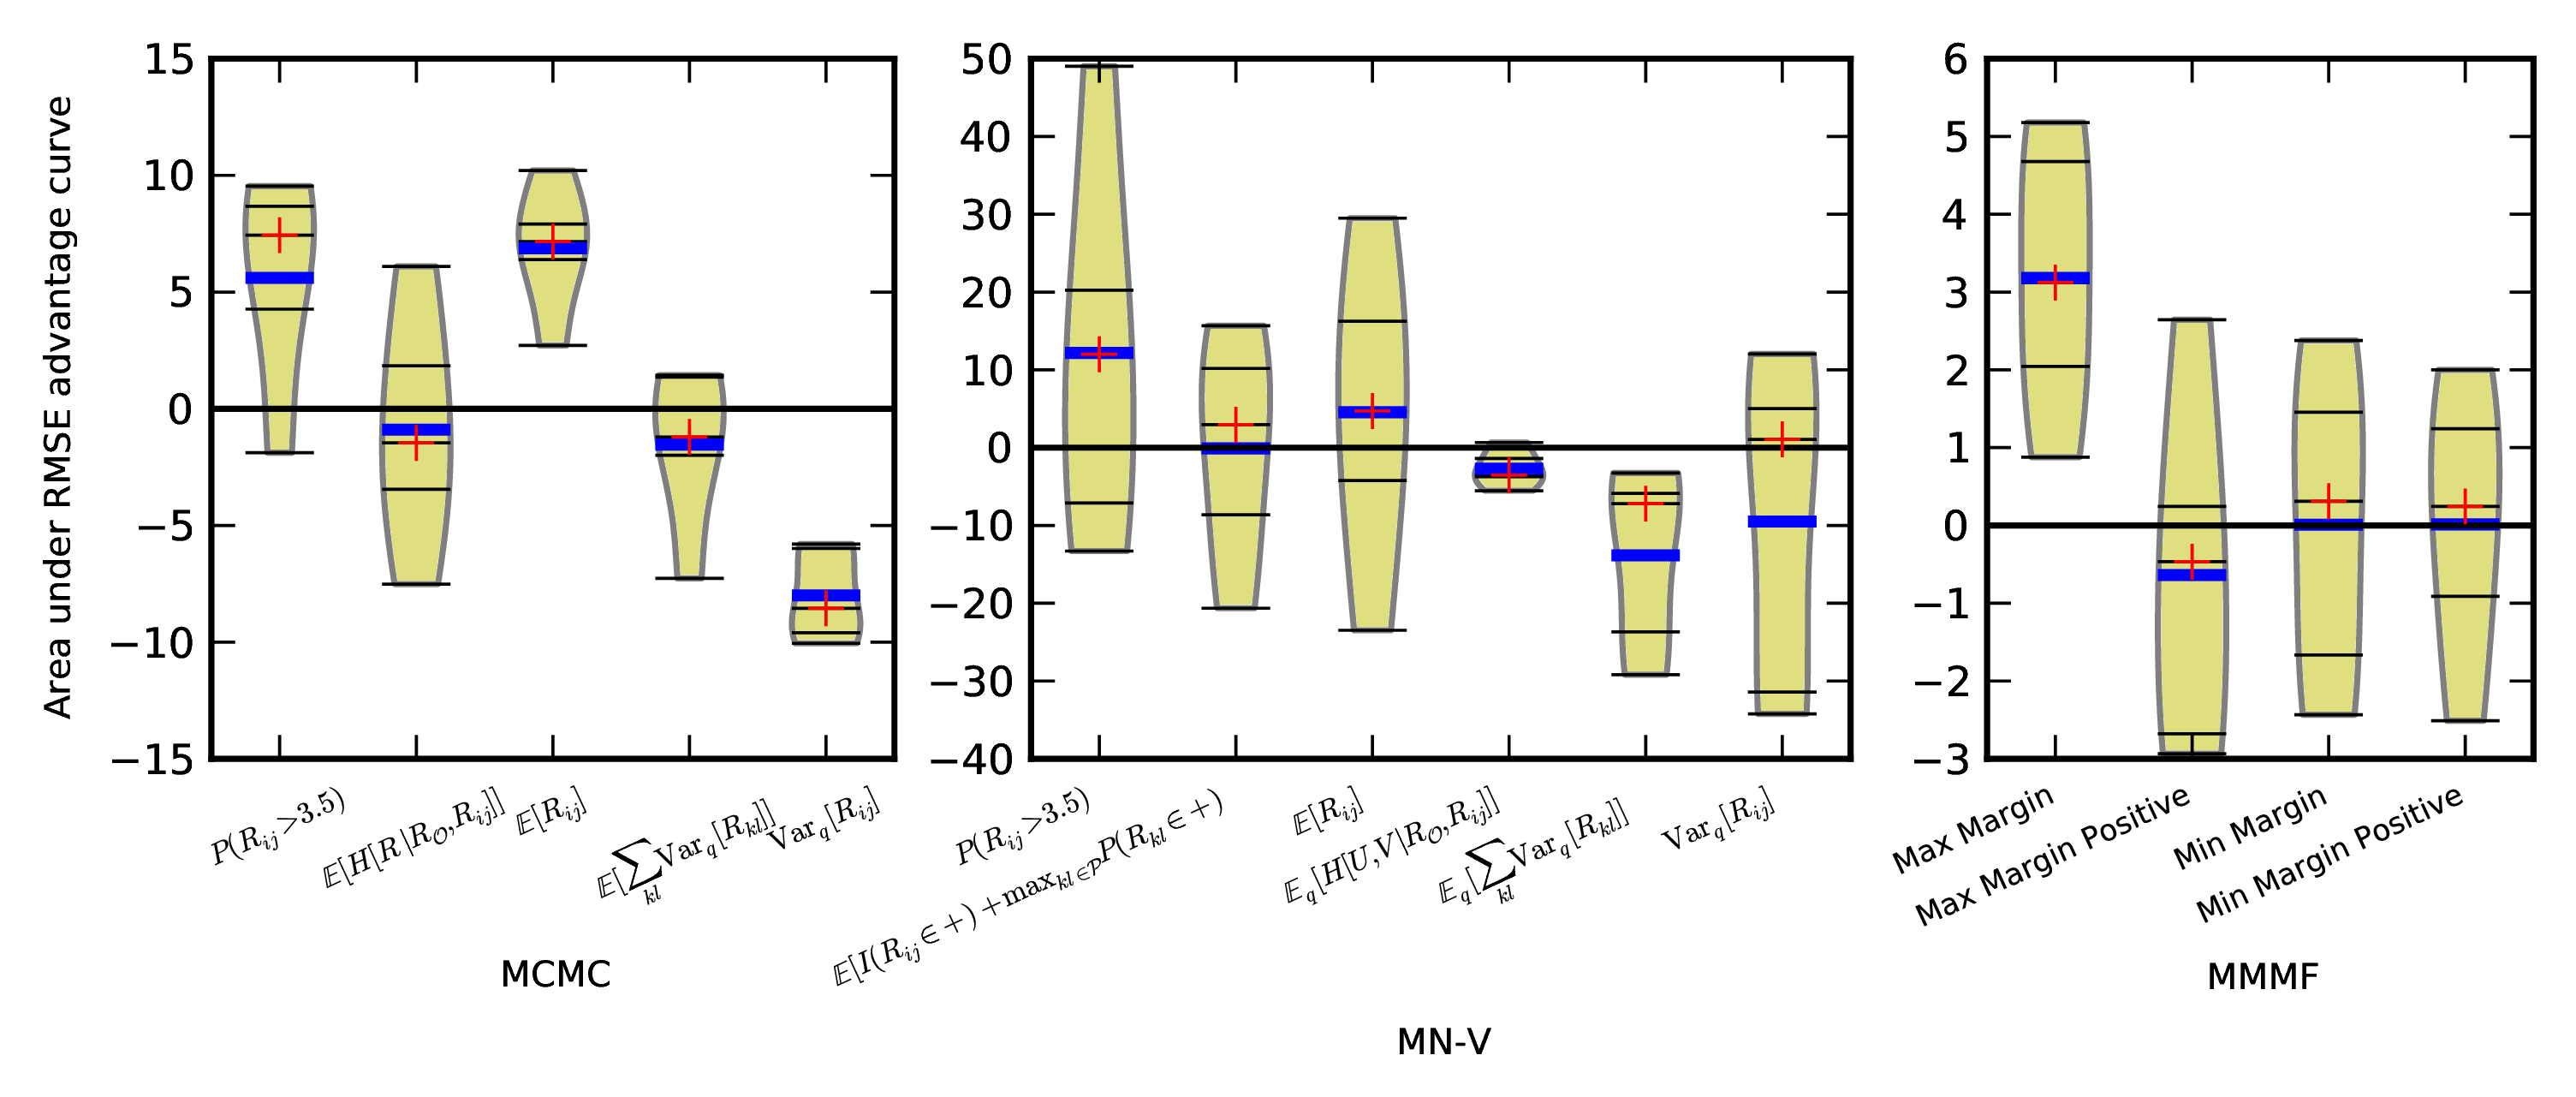
\includegraphics[width=\textwidth]{SutherlandPerformance}
    \else
      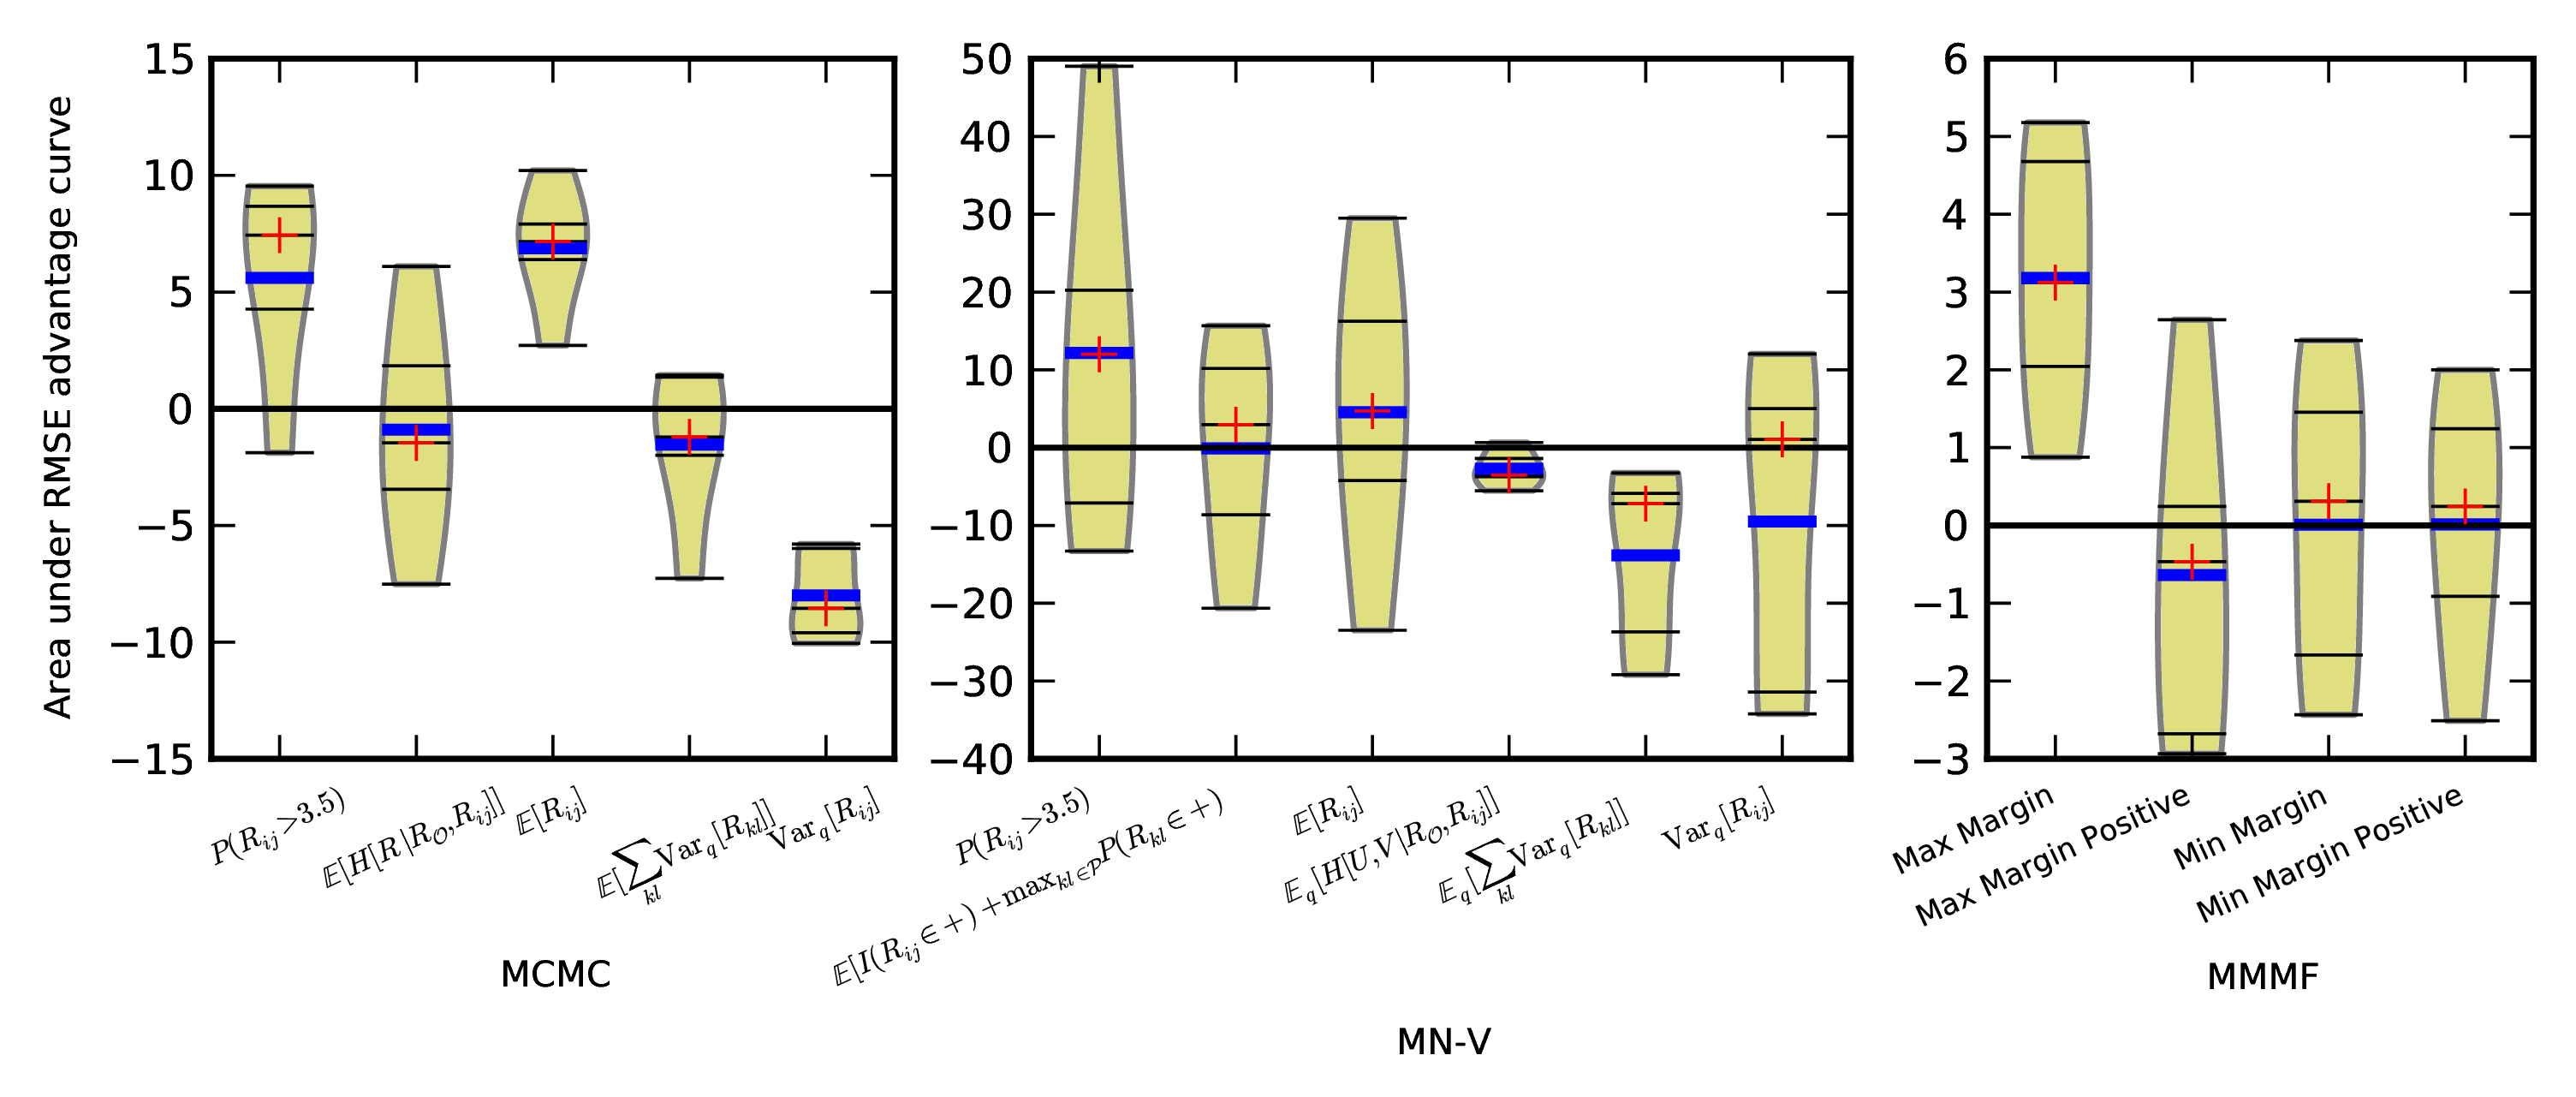
\includegraphics[bb = 92 86 545 742, width=\textwidth]{SutherlandPerformance}
    \fi
    \end{center}
This figure from Sutherland et al.'s paper \cite{active-mf} gives the prediction results of various techniques observed. The Area under RMSE advantage curve values represent the results of five runs of a $10 \times 10$ rank 1 continuous synthetic experiment against random sampling. Thus a negative value represents a method outperforming random selection.
  \begin{center}
    \leavevmode
    \ifpdf
      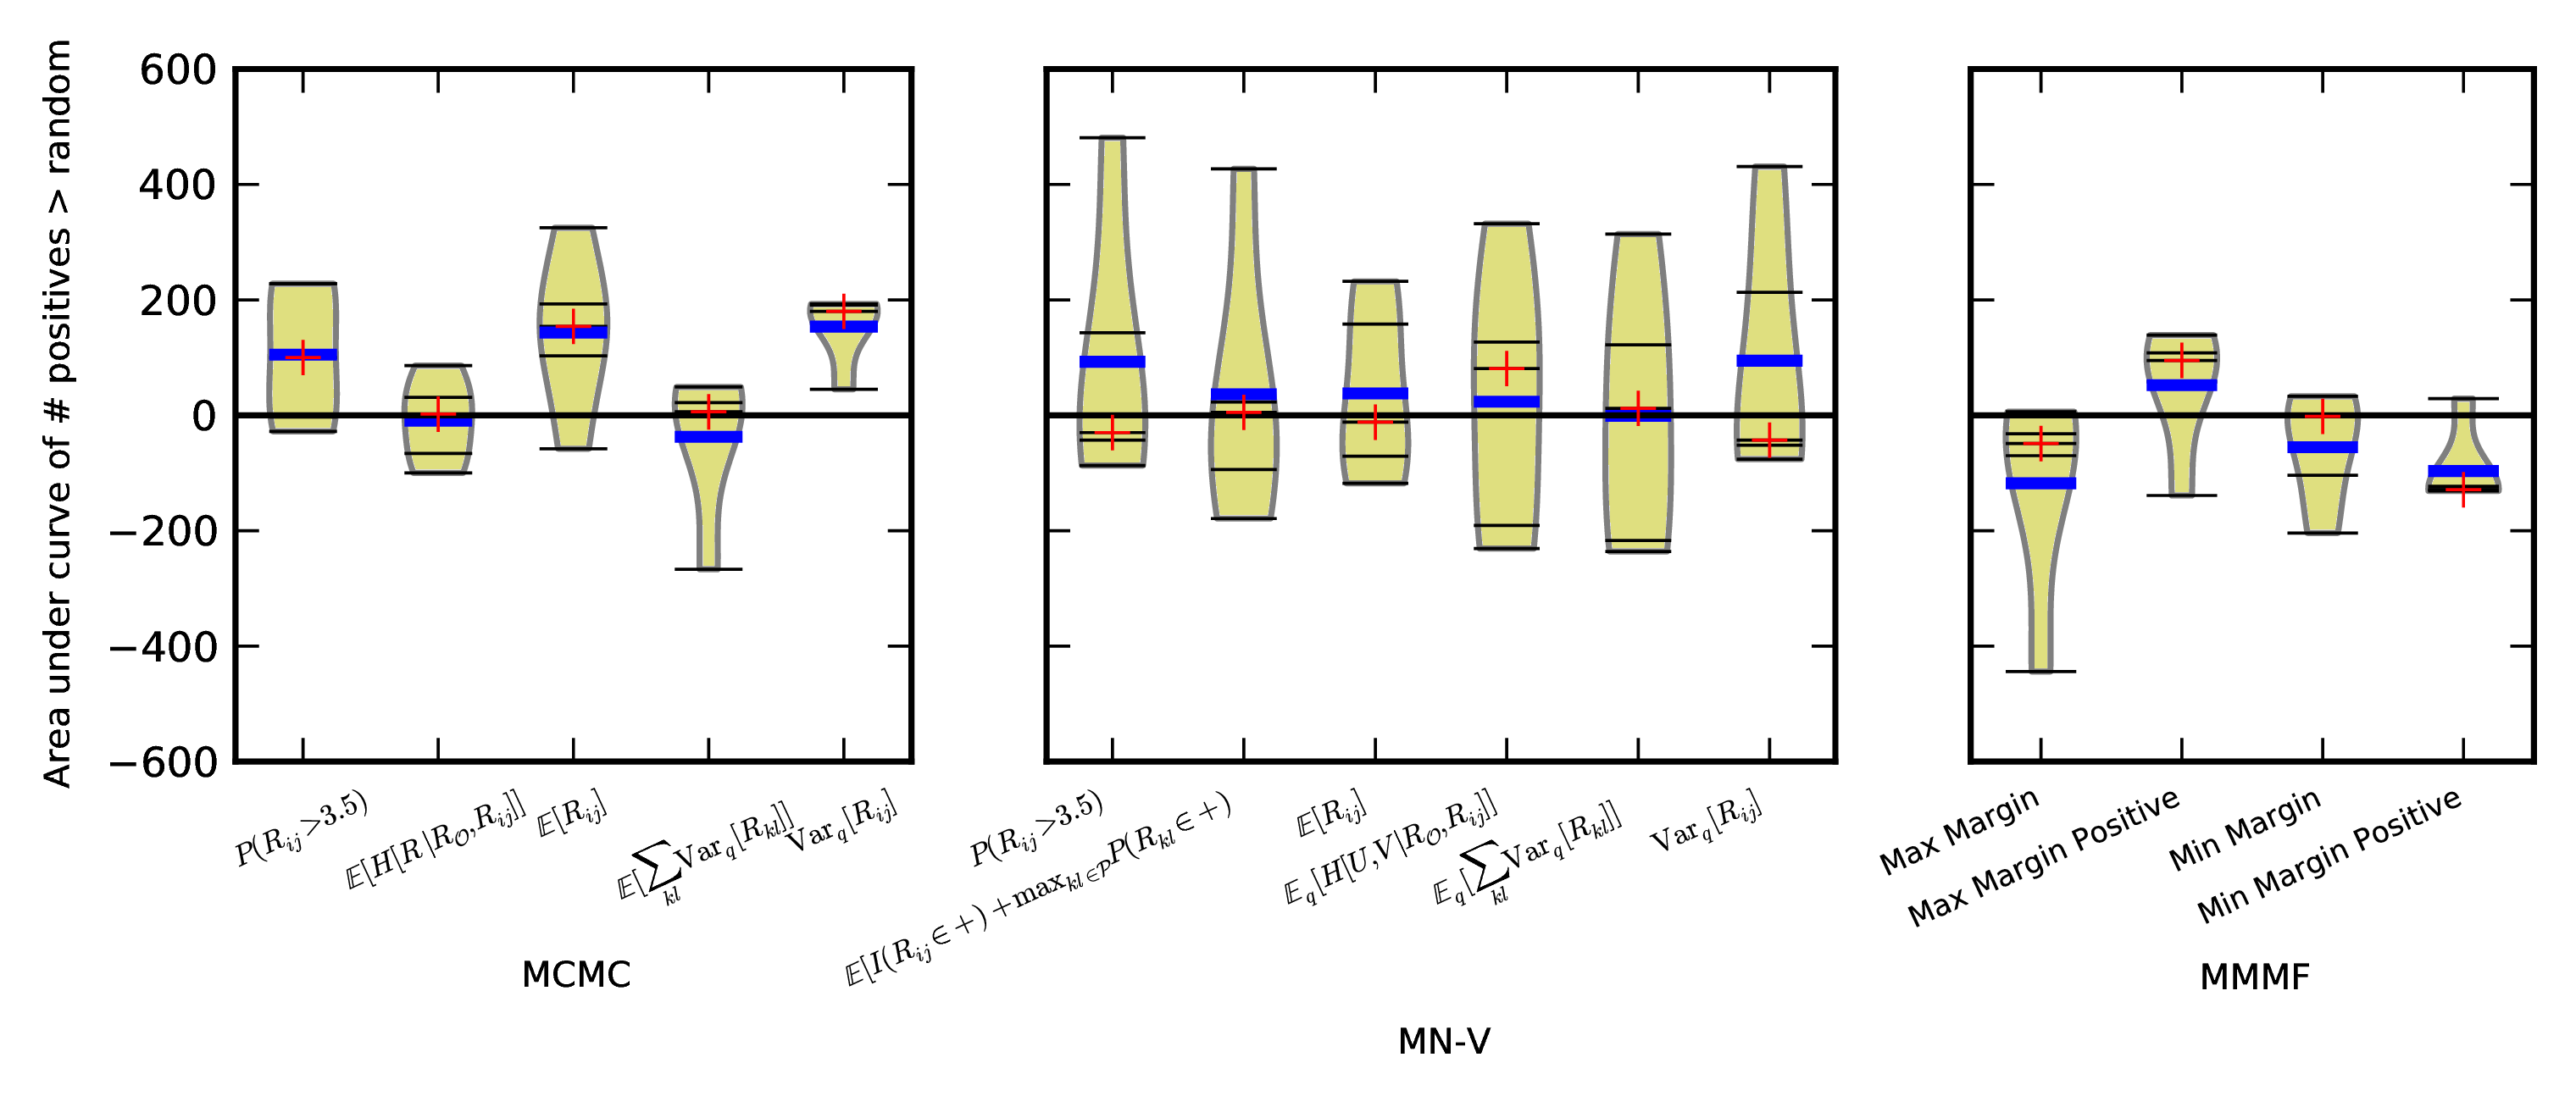
\includegraphics[width=\textwidth]{SutherlandPerformance_disc}
    \else
      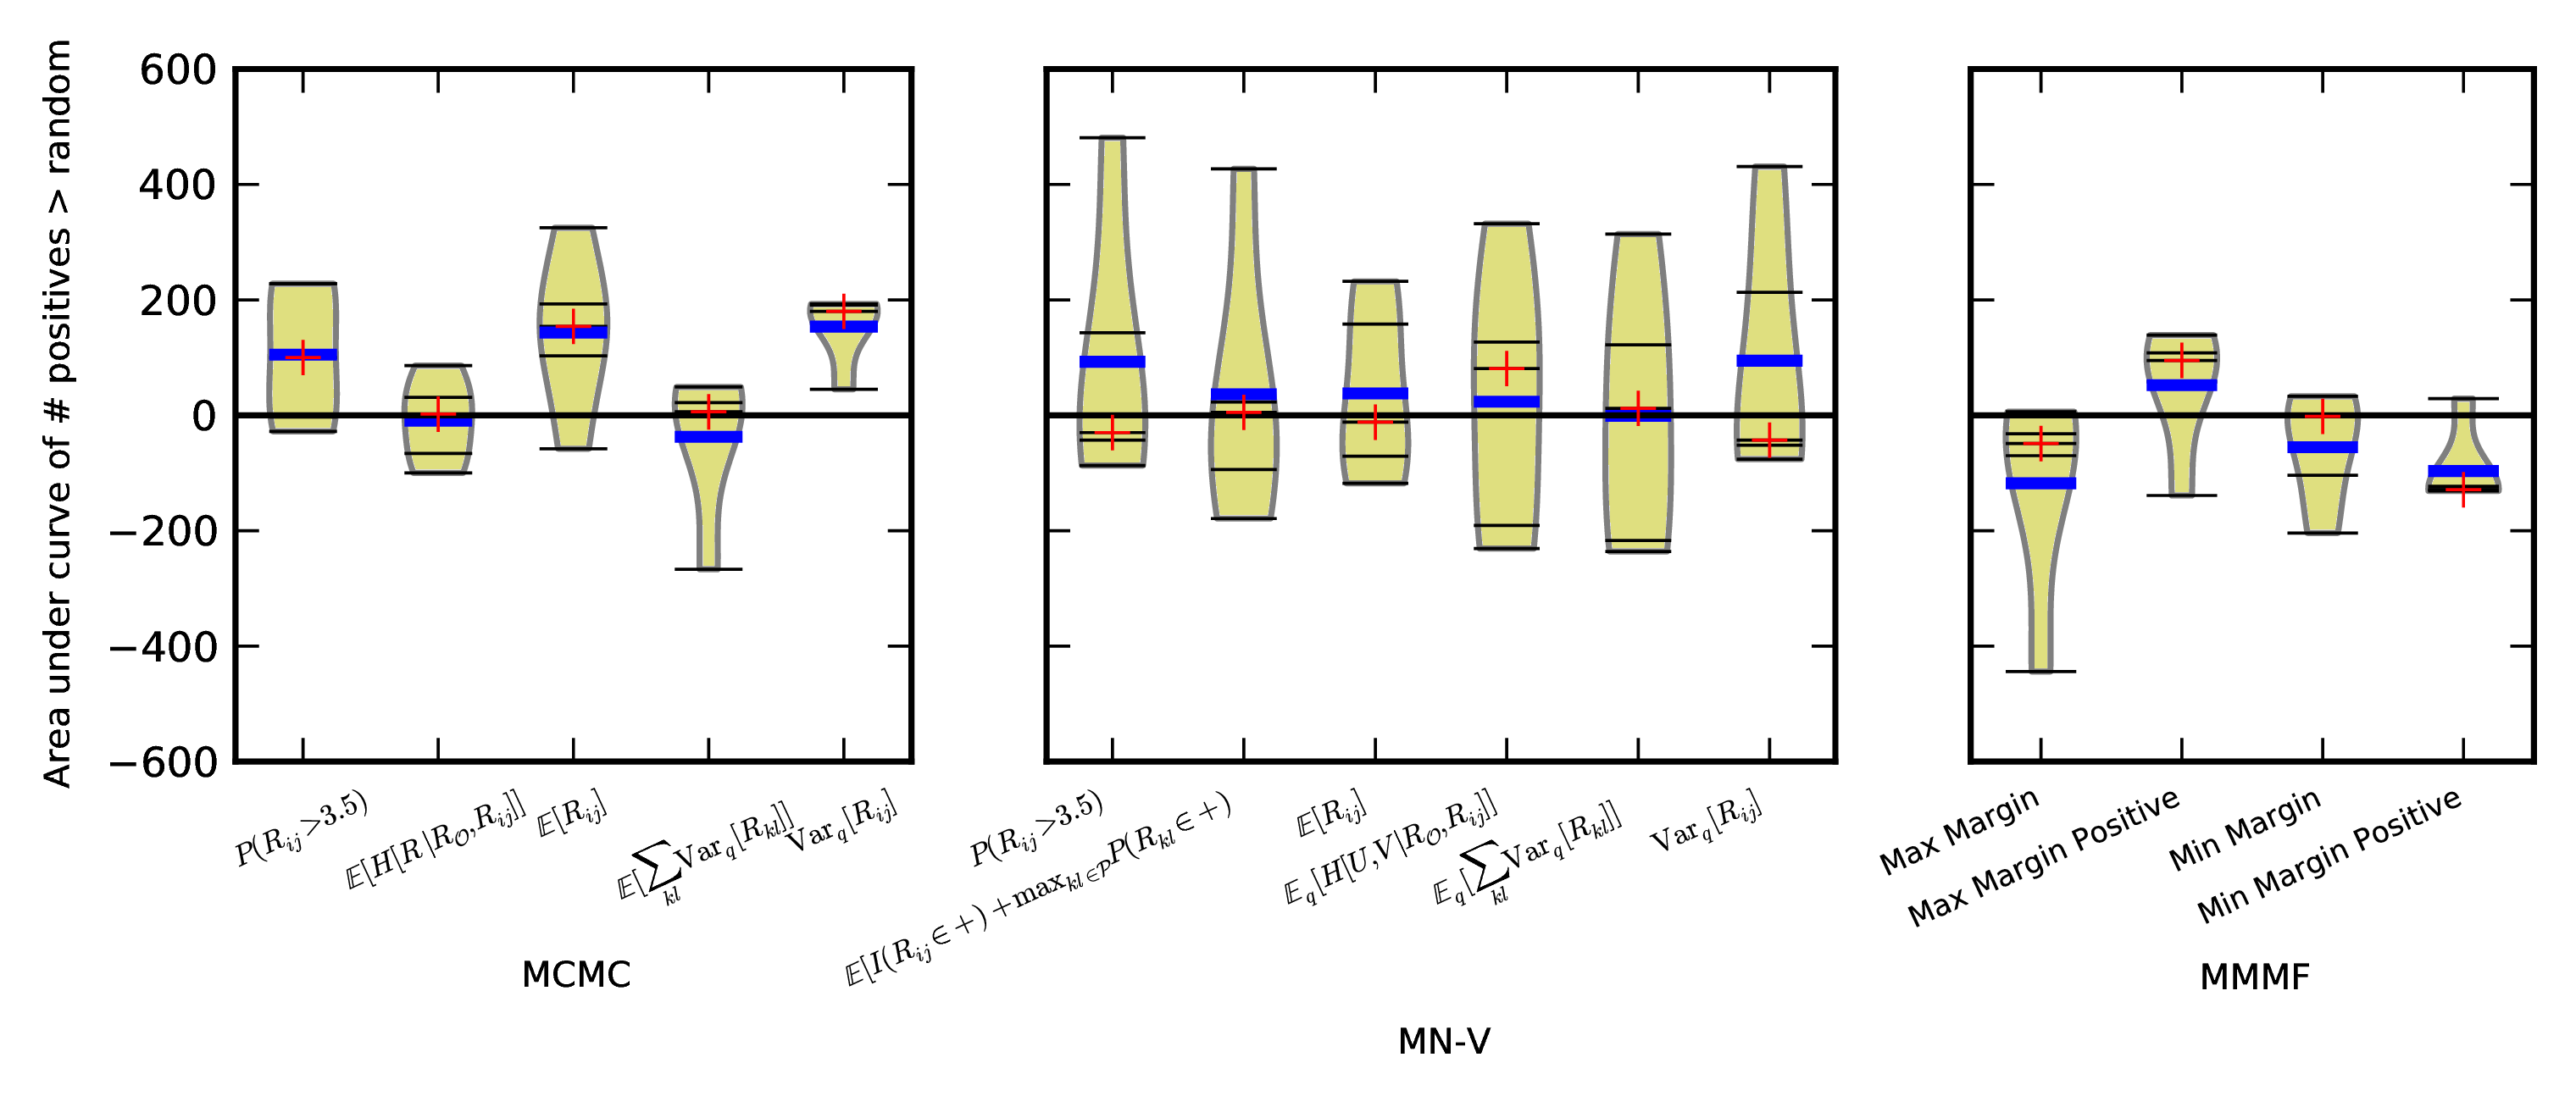
\includegraphics[bb = 92 86 545 742, width=\textwidth]{SutherlandPerformance_disc}
    \fi
    \end{center}
This figure gives the prediction results of various techniques observed for a synthetic discrete dataset. This time the measure is the number of useful values queried in a  $10 \times 10$ rank 4 discrete synthetic experiment against random sampling. A positive value represents a method outperforming random selection.

    \caption{Outline of the performance of algorithms proposed by Sutherland et al.}
    \label{fig:sutherland_alg}
\end{figure}
\nomenclature{MN-V}{Matrix-Normal Variational framework - Variational inference of the probability distribution of data in a matrix assuming Gaussian distribution}

\nomenclature{MMMF}{Maximum Margin Matrix Factorization - A collaborative prediction algorithm using low-norm instead of low-rank factorizations}

As can be seen, not all proposed methods performed well and even underperformed random selection. For this reason all Maximum Margin Matrix Factorization based methods are ignored, having little significant improvement over random selection. The two methods that exhibited good performance over the discrete and continuous datasets where the $\mathrm{Var}[R_{ij} \mid R_\mathcal{O}]$ searches, under Matrix-Normal and MCMC approximations. Thus, these will be the two algorithms implemented to be tested.

\section{Matrix-Normal Variance Search}
\label{sec:mnvar}
Here the idea is to infer the variance of unknown samples to be able to choose a target. The variance is used as a proxy for uncertainty, where samples with a high variance are assumed to be the most "uncertain", due to being able to vary more.
\subsection{Derivation}
The value we seek for each sample is the variance of each individual sample given the observed set, that is $\mathrm{Var}[R_{ij} \mid R_\mathcal{O}]$. We derive it as such:
\begin{align*}
\mathrm{Var}[R_{ij} \mid R_\mathcal{O}] &= \mathbb{E} [\mathrm{Var}[R_{ij} \mid U,V] \mid R_\mathcal{O}] + \mathrm{Var} [\mathbb{E}[R_{ij} \mid U,V] \mid R_\mathcal{O}]\\
&= \mathbb{E}[\sigma^2] + \mathrm{Var}[\mathbf{u}_i^T \mathbf{v}_j \mid R_\mathcal{O}] \\
\mathrm{Var}[\mathbf{u}_i^T \mathbf{v}_j \mid R_\mathcal{O}] &= \mathrm{Var}\left[\sum\limits_{k=1}^{D} U_{ik}V_{jk} \mid R_\mathcal{O}\right] \\
&= \sum\limits_{k=1}^{D} \sum\limits_{l=1}^{D} \mathrm{Cov}[U_{ik}V_{jk},U_{il}V_{jl} \mid R_\mathcal{O}] \\
&= \sum\limits_{k=1}^{D} \sum\limits_{l=1}^{D} \mathbb{E}[U_{ik}V_{jk}U_{il}V_{jl} \mid R_\mathcal{O}] - \mathbb{E}[U_{ik}V_{jk} \mid R_\mathcal{O}] \mathbb{E}[U_{il}V_{jl} \mid R_\mathcal{O}]\\
\end{align*}


As $\mathbb{E}[\sigma^2]$ is a constant, we can ignore it. Now $\mathbb{E}[U_{ik}V_{jk} \mid R_\mathcal{O}]$ and $\mathbb{E}[U_{il}V_{jl} \mid R_\mathcal{O}]$ are not yet usable in their current form, we find their value via:
\begin{align*}
\mathbb{E}[X_a X_b] = \mathbb{E}[X_a] \mathbb{E}[X_b] + \mathrm{Cov}[X_a, X_b] = \mu_a\mu_b + \Sigma_{a,b}
\end{align*}
Where $\Sigma_{a,b}$ is the covariance matrix -  $\Sigma_{ab}= \mathrm{Cov}(X_a, X_b) = \mathbb{E}\left[
(X_a - \mu_a)(X_b - \mu_b)\right]$

The expression for $\mathbb{E}[U_{ik}V_{jk}U_{il}V_{jl} \mid R_\mathcal{O}]$ is slightly more complicated and requires the use of Isserlis' theorem \cite{isserlis1918}. Note that it assumes the random variables used are normal. 
\begin{align*}
\mathbb{E}[X_aX_bX_cX_d] &= \mu_a\mu_b\mu_c\mu_d +\mu_c\mu_d\Sigma{a,b}+\mu_b\mu_d\Sigma_{a,c}+\mu_b\mu_c\Sigma_{a,d}+\mu_a\mu_d\Sigma_{b,c}+\mu_a\mu_c\Sigma_{b,d}\\
&+\mu_a\mu_b\Sigma_{c,d} + \Sigma_{a,b}\Sigma_{c,d} + \Sigma_{a,c}\Sigma_{b,d} + \Sigma_{a,d}\Sigma_{b,c}
\end{align*}

To move from the $a,b,c,d$ coordinate system to $i,j,k,l$ to calculate $\mathrm{Var}[\mathbf{u}_i^T \mathbf{v}_j \mid R_\mathcal{O}]$ we create what is called the Matrix-Normal Framework approximation, which is a multivariate matrix assuming Gaussian distribution \cite{gupta1999matrix}.  For this we build a matrix system as such \cite{active-mf-slides}:
\begin{align}
\Sigma_{ij} = \mathrm{Cov}(\left[\begin{smallmatrix} U^T\\ V^T \end{smallmatrix}\right], \left[\begin{smallmatrix} U^T\\ V^T \end{smallmatrix}\right]) &=  
\begin{array}{c|c|c|c|c|c|c|c|c|}
  & \mathbf{u}_1 & \mathbf{u}_2 & \mathbf{u}_3 & \mathbf{u}_4 & \mathbf{u}_5 & \mathbf{v}_1 & \mathbf{v}_2 & \mathbf{v}_3 \\ \hline
\mathbf{u}_1  &  &   &   &   &   &  &  &  \\ \hline
\mathbf{u}_2 &  &   &   &   &   &  &  &  \\ \hline
\mathbf{u}_3  &  &   &   &   &   &  &  &  \\ \hline
\mathbf{u}_4  &  &   &   &   &   &  &  &  \\ \hline
\mathbf{u}_5  &  &   &   &   &   &  &  &  \\ \hline
\mathbf{v}_1  &  &   &   &   &   &  &  &  \\ \hline
\mathbf{v}_2  &  &   &   &   &   &  &  &  \\ \hline
\mathbf{v}_3  &  &   &   &   &   &  &  &  \\ \hline
\end{array} \label{eq:sigma_cov} \\
\Omega_{kl} =  \mathrm{Cov}(\left[\begin{smallmatrix} U & V \end{smallmatrix}\right], \left[\begin{smallmatrix} U & V \end{smallmatrix}\right]) &= 
\begin{array}{c|c|c|c|c|}
  & \mathbf{f}_1 & \mathbf{f}_2 & \mathbf{f}_3 & \mathbf{f}_4  \\ \hline
\mathbf{f}_1  &  &   &   &    \\ \hline
\mathbf{f}_2 &  &   &   &     \\ \hline
\mathbf{f}_3  &  &   &   &    \\ \hline
\mathbf{f}_4  &  &   &   &    \\ \hline
\end{array} \label{eq:omega_cov}
\end{align}

That is we assemble $U$ and $V$ into a single matrix and create the covariance matrices $\Sigma$ and $\Omega$. $\Sigma$ is the covariance of the features of each row ($U$) and column ($V$), thus $\Sigma \in \mathbb{R}^{(M+N)\times (M+N)}$. $\Omega$ is the covariance of the features themselves, thus $\Omega \in \mathbb{R}^{D\times D}$. This is used to get the full covariance matrix over all features of rows and columns by $\Sigma \otimes \Omega$.

From this we can consider $U$ and $V$ to be one variable, thus $\mathbb{E}[U_{ik}V_{jl}] = \mathbb{E}[X_{a}X_{b}]$ where $a = (i,j)$ and $b=(k,l)$. This gives:
\begin{align*}
\mathbb{E}[X_a X_b]  &= \mu_a\mu_b + \Sigma_{a,b}\\
&=\mathbb{E}[U_{ik}V_{jl}] = U_{ik}V_{jl} + \Sigma_{ij} \Omega_{kl}
\end{align*}
The indices $i,j$ refer to the $U,V$ coordinates in $\Sigma$ in equation \ref{eq:sigma_cov}. $k,l$ refers to the coordinates of the features of $\Omega$ in equation \ref{eq:omega_cov}. Note that the complexity to calculate $\Sigma$ and $\Omega$ combined is $O(D^3+(N+M)^3)$. Additionally note that $U_{ik}V_{jl}$ are used as means taken from the PMF best fit - while not ideal is an assumption required for calculation \cite{active-mf}.

\subsection{Performance}

This was first tested on the same $80\times 50$ synthetic data as in previous experiments and while the performance was good, it tended to "edge out" after more than 25\% of the dataset became available. A typical run is show in figure \ref{fig:MN-V-perf}. This is consistent with the performance reported by Sutherland et al. in figure \ref{fig:sutherland_alg}. 

  \begin{figure}[!htbp]
    \begin{center}
      \resizebox{\textwidth}{!}{% This file was created by matlab2tikz v0.4.7 running on MATLAB 8.1.
% Copyright (c) 2008--2014, Nico Schlömer <nico.schloemer@gmail.com>
% All rights reserved.
% Minimal pgfplots version: 1.3
% 
% The latest updates can be retrieved from
%   http://www.mathworks.com/matlabcentral/fileexchange/22022-matlab2tikz
% where you can also make suggestions and rate matlab2tikz.
% 
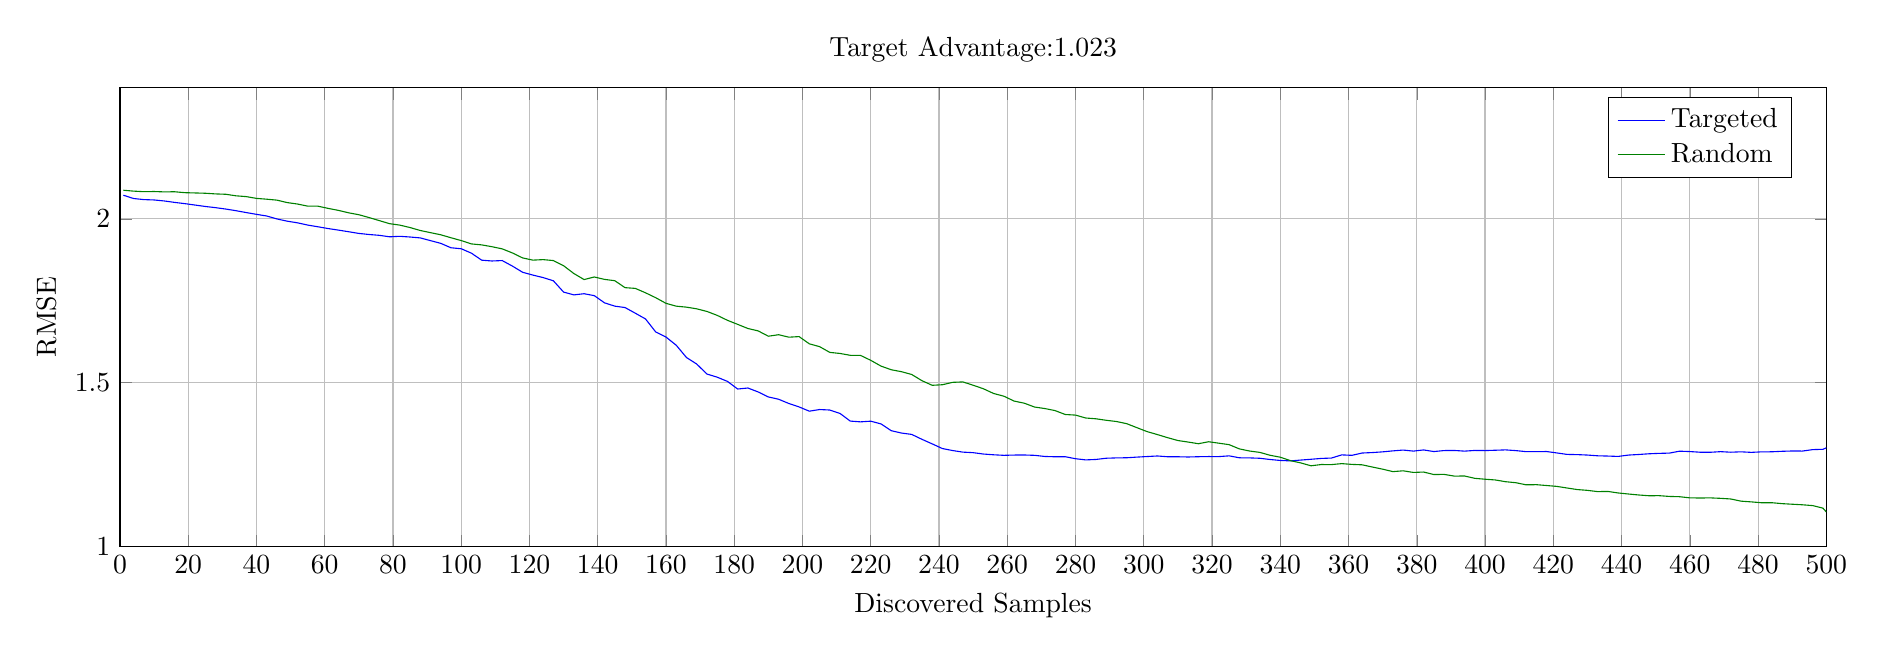
\begin{tikzpicture}

\begin{axis}[%
width=8.53186185641769in,
height=2.2921875in,
scale only axis,
xmin=0,
xmax=500,
xlabel={Discovered Samples},
xmajorgrids,
ymin=1,
ymax=2.4,
ylabel={RMSE},
ymajorgrids,
title={Target Advantage:1.023},
legend style={draw=black,fill=white,legend cell align=left}
]
\addplot [color=blue,solid]
  table[row sep=crcr]{1	2.07217796492918\\
4	2.06212270493792\\
7	2.05882437356678\\
10	2.05770772310212\\
13	2.05463256819977\\
16	2.05029038999817\\
19	2.04649955568304\\
22	2.04214711050768\\
25	2.03784797301423\\
28	2.03423279648376\\
31	2.02993729993713\\
34	2.02491635055087\\
37	2.01922342208279\\
40	2.01378732920106\\
43	2.00872741451322\\
46	1.99976064873121\\
49	1.99293235568156\\
52	1.98793139275403\\
55	1.98110244914886\\
58	1.97582861008334\\
61	1.97037647217666\\
64	1.96568743235825\\
67	1.96067642065653\\
70	1.95553225814245\\
73	1.95222363231337\\
76	1.94968837600179\\
79	1.94519452757987\\
82	1.94671582574677\\
85	1.94456924839872\\
88	1.94184800352677\\
91	1.93349583223219\\
94	1.92521848332823\\
97	1.91172130596277\\
100	1.90872882346895\\
103	1.8951253682236\\
106	1.87382958242028\\
109	1.87133938997235\\
112	1.87267011501452\\
115	1.85575306466301\\
118	1.83687065850172\\
121	1.82824122276525\\
124	1.82068993413038\\
127	1.81087884392425\\
130	1.77638745622223\\
133	1.76782438413003\\
136	1.77138943510964\\
139	1.76545820964674\\
142	1.74346779835438\\
145	1.73344175033161\\
148	1.72913726284919\\
151	1.71195929165539\\
154	1.69433936018818\\
157	1.65448344243473\\
160	1.63908694767779\\
163	1.61406681384958\\
166	1.57657630015616\\
169	1.5566917565721\\
172	1.52609994092278\\
175	1.51652904610699\\
178	1.50368856939048\\
181	1.48034402085276\\
184	1.4834528761387\\
187	1.47143288411547\\
190	1.45616474257825\\
193	1.44914891665654\\
196	1.43612670123312\\
199	1.4256581573023\\
202	1.41268358703128\\
205	1.41771340661325\\
208	1.41622550427769\\
211	1.40570120787203\\
214	1.38237721813787\\
217	1.38011853506596\\
220	1.3821246187814\\
223	1.37381796929417\\
226	1.35312809052608\\
229	1.34590495237109\\
232	1.34172684008272\\
235	1.32677225750146\\
238	1.3128521315865\\
241	1.2985509003513\\
244	1.29244945131536\\
247	1.28763987729826\\
250	1.28600061641922\\
253	1.28182325718132\\
256	1.27951413932043\\
259	1.27785169964859\\
262	1.27868774427141\\
265	1.27889345984466\\
268	1.27784137986272\\
271	1.27440947077995\\
274	1.27345121745604\\
277	1.2735928261685\\
280	1.26750193622842\\
283	1.26391104521067\\
286	1.26528659700911\\
289	1.26901035717902\\
292	1.27001218520397\\
295	1.27045536007768\\
298	1.27244298118008\\
301	1.2741919126503\\
304	1.27586897349281\\
307	1.27351270608901\\
310	1.27347313801709\\
313	1.27278813577858\\
316	1.27363043193357\\
319	1.27414402457253\\
322	1.27397896515088\\
325	1.27627622196343\\
328	1.27034812716924\\
331	1.27000627074729\\
334	1.2688956149271\\
337	1.26510646390248\\
340	1.26219130517703\\
343	1.2609059246488\\
346	1.26338860069923\\
349	1.26582053648389\\
352	1.26838961520604\\
355	1.26955477380922\\
358	1.27923001828898\\
361	1.27787091977098\\
364	1.28491935067654\\
367	1.28632801279594\\
370	1.2884657736677\\
373	1.29146883806027\\
376	1.29393893355191\\
379	1.29077127223434\\
382	1.29432065066798\\
385	1.28937288250242\\
388	1.29241691857647\\
391	1.2926933454363\\
394	1.29068756028848\\
397	1.29278769210034\\
400	1.29239303326408\\
403	1.29338884344584\\
406	1.2944748838647\\
409	1.29229343793145\\
412	1.28914655804349\\
415	1.28899567267332\\
418	1.28948087633663\\
421	1.28524664406664\\
424	1.28067337280748\\
427	1.28003038581361\\
430	1.2786961804855\\
433	1.27642714256949\\
436	1.27562242107382\\
439	1.27450140845304\\
442	1.27861911267101\\
445	1.28040813099069\\
448	1.28257635215677\\
451	1.28385629785686\\
454	1.28464215850466\\
457	1.29051195243648\\
460	1.28936667759647\\
463	1.28736885772353\\
466	1.28715448817792\\
469	1.28908509561051\\
472	1.28738485746969\\
475	1.28857929723097\\
478	1.2868948476176\\
481	1.28845828893595\\
484	1.2886646594279\\
487	1.29015662030612\\
490	1.29112064688728\\
493	1.29087869993448\\
496	1.29532409422768\\
499	1.29620725378601\\
500	1.30079161418323\\
};
\addlegendentry{Targeted};

\addplot [color=black!50!green,solid]
  table[row sep=crcr]{1	2.08737177550677\\
4	2.08467184403021\\
7	2.08298650087891\\
10	2.08348084945761\\
13	2.08235832565932\\
16	2.08278336567022\\
19	2.07997182596675\\
22	2.07911563225928\\
25	2.07822621974444\\
28	2.07619799809029\\
31	2.07509690461574\\
34	2.07037368540558\\
37	2.06796467565784\\
40	2.06249287777274\\
43	2.06005976089149\\
46	2.05720714465723\\
49	2.0496930022108\\
52	2.04530723149985\\
55	2.03888774106181\\
58	2.03873361093176\\
61	2.03199201729195\\
64	2.02591876819778\\
67	2.01848311414454\\
70	2.01262361605077\\
73	2.00395155190626\\
76	1.99462540594667\\
79	1.9852882756053\\
82	1.98091641778124\\
85	1.97347796749868\\
88	1.96446618648546\\
91	1.95785514086079\\
94	1.95138422004017\\
97	1.94229146720604\\
100	1.93366901648982\\
103	1.92342241018382\\
106	1.92051777604366\\
109	1.91496899516326\\
112	1.90839163752708\\
115	1.89586488086919\\
118	1.88066140255096\\
121	1.87395392292007\\
124	1.87550781674251\\
127	1.87264828173258\\
130	1.85683936289269\\
133	1.83307619089402\\
136	1.81464118524864\\
139	1.82249171408737\\
142	1.81510203517035\\
145	1.81115487870425\\
148	1.78991566680894\\
151	1.78768268232496\\
154	1.77419933459181\\
157	1.75914470656101\\
160	1.74201480568861\\
163	1.73337351081135\\
166	1.73037832871174\\
169	1.72524028710671\\
172	1.7172640519419\\
175	1.70530684126998\\
178	1.69022289382998\\
181	1.67781688837803\\
184	1.6651866018857\\
187	1.65786833325152\\
190	1.64163461056598\\
193	1.64621427296132\\
196	1.6386410457844\\
199	1.64045407738492\\
202	1.61837347420205\\
205	1.60981307131975\\
208	1.59221952958318\\
211	1.58892920883708\\
214	1.58329322993786\\
217	1.58301614026078\\
220	1.567965103681\\
223	1.55038370751194\\
226	1.53919574761702\\
229	1.53327736766467\\
232	1.52476495571093\\
235	1.50581086034833\\
238	1.49171998420279\\
241	1.49342951724959\\
244	1.5007717380585\\
247	1.50204426605883\\
250	1.49192696470451\\
253	1.48121566474336\\
256	1.46672052014451\\
259	1.45844805265428\\
262	1.44355779059618\\
265	1.43703738035327\\
268	1.4253302052287\\
271	1.42074401790011\\
274	1.41449212897748\\
277	1.40253724549153\\
280	1.40069222665835\\
283	1.39180532175089\\
286	1.38940725648008\\
289	1.38487970543042\\
292	1.38110597813458\\
295	1.3745230010058\\
298	1.36230351141792\\
301	1.3501871378517\\
304	1.3412095644929\\
307	1.33173351861769\\
310	1.32304550636488\\
313	1.31840292381511\\
316	1.31334104190201\\
319	1.31933152266431\\
322	1.31495091989763\\
325	1.31047964925082\\
328	1.29756420173432\\
331	1.29097480308478\\
334	1.28685145817632\\
337	1.27805122623317\\
340	1.27212012515377\\
343	1.26156765537743\\
346	1.2546533090913\\
349	1.2459105816125\\
352	1.24972460480505\\
355	1.24957136202949\\
358	1.25251678013392\\
361	1.25017249793226\\
364	1.24889540351554\\
367	1.24207233711686\\
370	1.23558814397032\\
373	1.22809686061264\\
376	1.23060254216309\\
379	1.22558605980194\\
382	1.22682227549603\\
385	1.21920191679697\\
388	1.21968643397675\\
391	1.21442053358153\\
394	1.21472677378805\\
397	1.2076025372052\\
400	1.20488826736279\\
403	1.20264160565174\\
406	1.19732675748935\\
409	1.19427745019973\\
412	1.18787560986912\\
415	1.18824687142166\\
418	1.18569285163679\\
421	1.18301310411735\\
424	1.17815756614337\\
427	1.1733234895432\\
430	1.170920066358\\
433	1.16705564895868\\
436	1.16758311592514\\
439	1.16291304863818\\
442	1.15974434515618\\
445	1.15677495393665\\
448	1.15445458443966\\
451	1.15467135208282\\
454	1.15233728237269\\
457	1.15149389611694\\
460	1.1479855493612\\
463	1.14753512073225\\
466	1.14791346977819\\
469	1.14654344230593\\
472	1.14456063957849\\
475	1.13791032233366\\
478	1.13570570496753\\
481	1.13306893975319\\
484	1.13318773014601\\
487	1.13032176593801\\
490	1.12855069123371\\
493	1.12682279115302\\
496	1.12434455628116\\
499	1.11658124448945\\
500	1.10494857330348\\
};
\addlegendentry{Random};

\end{axis}
\end{tikzpicture}%}
    \end{center}
    Performed on Synthetic Data.
      \caption{Matrix Normal Maximum Variance Search}
      \label{fig:MN-V-perf}
  \end{figure}
  
  
\subsubsection{Improving Performance}

Calculating the variance has a complexity of about $O(MND^2)$ in addition to the calculation of the covariance matrices, thus calculating the criteria at each new sample is not ideal. These tweaks were done to improve performance: 

\begin{description}[style=standard,leftmargin=.7cm,font=\bfseries]
  \item[Variance Matrix Calculation Update] Rather than calculating the matrix everytime a new sample comes in, we calculate the matrix at fixed intervals of incoming samples, for example after 10 have been requested.
  \item[Memory Optimisation] There are many combinations of $\mathbb{E}[U_{ik}V_{jl}]$ over the double summation. To optimise, we use the symmetry property of the covariance matrix and locally cache already calculated values.
  \item[Unknown Samples] We only calculate the variance for unknown samples.
  \item[Online Updating] When $U$ and $V$ are calculated online it is also possible to gradually update the variance matrix.

\end{description}

Basic memory optimisation alone allowed the execution to be more than halved. In the case of a $80 \times 50$ matrix with $D=7$, from 1.81 seconds down to 0.81 seconds on average.


\section{MCMC Variance Search}
\label{sec:mcmcvar}
From results obtained in simulations as well as Sutherland et al.'s we saw that the Matrix-Normal Variance Search performed reasonably well, but had instances of under performing random selection. One of the reasons for this was that the data distribution was not entirely reflected in $U$ and $V$ used to calculate $\mathrm{Var}[\mathbf{u}_i^T \mathbf{v}_j \mid R_\mathcal{O}]$. 
\subsection{Derivation}
Here we keep the same equations for $\mathrm{Var}[\mathbf{u}_i^T \mathbf{v}_j \mid R_\mathcal{O}]$ but instead take $U$ and $V$ from an estimate sampled across the expected distribution of data. In BPMF, section \ref{sec:bpmf}, we had $U$ and $V$ expressed as:

\begin{align*}
P(U,V|R,\Theta_U,\Theta_V) =\int \int P(R | U,V) P(U,V | R,\Theta_U,\Theta_V) P(\Theta_U,\Theta_V | \Theta_0)d\Theta_U d\Theta_V
\end{align*}

Unfortunately an analytical solution is difficult to achieve and we instead rely on approximation methods. For quick intuition on how this works consider the following, simplified, function \cite{mcmc-int}:
\begin{align*}
I = \int g(\theta)p(\theta)d\theta
\end{align*}
Where $g(\theta)$ is a function of $\theta$ and $p(\theta)$ is the distribution of this variable. In cases where this is not possible we resort to Monte-Carlo Markov Chain Integration:
\begin{align*}
\hat{I}_M =\frac{1}{M} \sum\limits_{i=1}^{M} g(\theta ^{(i)}) 
\end{align*}

Where $M$ is the number of values sampled and $i$ the index. We have that as $M \to \infty$, $\hat{I}_M = I$. By process of iteration and random sampling the real distribution is approached and $\hat{I}_M$ is used instead of $I$.This is the process we will use to sample from the already known values.


 Sutherland et al.\cite{active-mf} use Hamiltonian Monte Carlo sampling methods but here we will use Gibbs Sampling, in a similar way to Salakhutdinov and Mnih \cite{SalMnih2008} in BPMF. Algorithm \ref{alg:gibbs_pmf} describes the process to sample from $V$, which is exactly the same for $U$. A $U$ and $V$ obtained via PMF are used as inputs.


\begin{algorithm}
\caption{Gibbs Sampling for BPMF}\label{alg:gibbs_pmf}
\begin{algorithmic}[1]
\Procedure{GibbsSamplingForV}{$U$,$V$,$R$}
\For{j=1..M} 
\State{$row_{in} = $row indices of known samples in column $j$} 
\State{$\mathcal{M} = U_{index = row_{in}}$} \Comment{Get feature vectors of known rows in column $j$}
\State{$\mathbf{r} = R_{row_{in},j}$} \Comment{Vector of known values in column $j$}
\State{$C = (\alpha_V+\beta\cdot\mathcal{M}^T\mathcal{M})^{-1}$} \Comment{Covariance of known feature vectors $U$}
\State{$\mu_V = C\cdot(\beta\cdot\mathcal{M}^T\mathbf{r}+\alpha_V \mu_V)$} \Comment{Update mean vector}
\State{$\Lambda = \text{Cholesky}(C)$} \Comment{Cholesky upper triangular decomposition}
\State{$\mathbf{x} \sim \mathcal{N}(0,1) \in \mathbf{R}^D$} \Comment{Randomly sample $D$ variables from Normal}
\State{$V_{j}=\Lambda\mathbf{x}+\mu_V$} \Comment{Update $V$}
\EndFor
\State \textbf{return} $V$
\EndProcedure
\end{algorithmic}
\end{algorithm}


$\alpha_V$ is the precision hyperparameter for $V$ and it is used to ensure non-singularity of $C$. $\mu_V$ is the average vector. $\beta$ is a parameter used for the Inverse-Wishart distribution, used as the prior of covariance matrix from data assumed to be from a normal distribution. Details are available in the appendix \ref{sec:app_bpmf}. We take $\Lambda$ as the Cholesky decomposition of the covariance $C$. If applied to a vector of uncorrelated samples ($\mathbf{x}$) it produces a vector with covariances of sampled system, which is why we add it to $\mu_V$, creating a feature vector of the samples.  Note that hyperparameters are reinitialised each loop before sampling trials.


In simpler terms, we capture the properties of the current distribution of known values in $V_j$ in $C$ and using the Cholesky decomposition update V with samples randomly generated from the captured distribution. Repeating this a few times(for our case, 3) over $U$ and $V$ asymptotically captures the real distribution of the samples. 

From this we get a better estimate of $\mathrm{Var}[\mathbf{u}_i^T \mathbf{v}_j \mid R_\mathcal{O}]$ and select the highest value for sampling.
\subsection{Performance}

MCMC Maximum Variance search was done on figure \ref{fig:MN-V-varsearch} and \ref{fig:eiffel_max_var_search}. As we see the performance on the synthetic data was better than the Matrix Normal version, being able to always perform better than random sampling. It should be noted that for image discovery, as in \ref{fig:eiffel_max_var_search}, MCMC performed less well than the clustered search (compare to figure \ref{fig:eiffel_clustering_random}) - this was observed over multiple runs. Finally the running speed was found to be quite a lot slower, taking 0.8 seconds on average compared to 0.01 for clustered knowledge search to calculate the criteria for sample selection.

 \begin{figure}[!htbp]
   \begin{center}
     \resizebox{\textwidth}{!}{% This file was created by matlab2tikz v0.4.7 running on MATLAB 8.1.
% Copyright (c) 2008--2014, Nico Schlömer <nico.schloemer@gmail.com>
% All rights reserved.
% Minimal pgfplots version: 1.3
% 
% The latest updates can be retrieved from
%   http://www.mathworks.com/matlabcentral/fileexchange/22022-matlab2tikz
% where you can also make suggestions and rate matlab2tikz.
% 
\begin{tikzpicture}

\begin{axis}[%
width=2.19625603864734in,
height=2.2728125in,
scale only axis,
xmin=0,
xmax=500,
xlabel={Discovered Samples},
xmajorgrids,
ymin=1,
ymax=2.4,
ylabel={RMSE},
ymajorgrids,
name=plot2,
title={Target Advantage:1.101}
]
\addplot [color=blue,solid,forget plot]
  table[row sep=crcr]{1	2.06951517257059\\
4	2.0869975872509\\
7	2.08103952147042\\
10	2.0753586370514\\
13	2.07373094997347\\
16	2.07115788724271\\
19	2.06963278760257\\
22	2.06484829701644\\
25	2.05728474072855\\
28	2.05841876874843\\
31	2.05142040393897\\
34	2.04438283782421\\
37	2.0358378827621\\
40	2.03712717447943\\
43	2.03731928304517\\
46	2.04154246089513\\
49	2.0350907696424\\
52	2.03828846856109\\
55	2.04488617363075\\
58	2.03879522020787\\
61	2.03363206341838\\
64	2.00987760912885\\
67	1.99602788609993\\
70	1.97164138282284\\
73	1.95054864630478\\
76	1.92469610058144\\
79	1.91853158115475\\
82	1.90193328286329\\
85	1.90425862662948\\
88	1.91152026099947\\
91	1.91217207143605\\
94	1.89405756567734\\
97	1.88021435737431\\
100	1.86702306784919\\
103	1.84463901382843\\
106	1.81318359279943\\
109	1.77777954157781\\
112	1.74438394947764\\
115	1.73044030606485\\
118	1.68282482446093\\
121	1.68032799007376\\
124	1.64103715043388\\
127	1.62711314432135\\
130	1.60059786692634\\
133	1.6086073738429\\
136	1.60612772446024\\
139	1.57532684746015\\
142	1.57555558858191\\
145	1.60443069661882\\
148	1.6107264530929\\
151	1.59633161832539\\
154	1.59486975503252\\
157	1.60186704616335\\
160	1.59132800396157\\
163	1.57979444828184\\
166	1.55327712016505\\
169	1.52695020217204\\
172	1.48503561723383\\
175	1.46361196222446\\
178	1.42633534386435\\
181	1.3815195130784\\
184	1.35763139007661\\
187	1.3433293607386\\
190	1.34505611035272\\
193	1.34927391157997\\
196	1.33406699947773\\
199	1.34399067458741\\
202	1.34685210142679\\
205	1.34451743747387\\
208	1.33006709754534\\
211	1.31551394501568\\
214	1.31408054120038\\
217	1.29917342848288\\
220	1.2838708773734\\
223	1.28473716486946\\
226	1.27931207133722\\
229	1.27470806417715\\
232	1.27130976104606\\
235	1.2681680675065\\
238	1.27643001273846\\
241	1.27056735500564\\
244	1.27003699360378\\
247	1.26237545338544\\
250	1.25315174140016\\
253	1.24710990204099\\
256	1.24399576780197\\
259	1.24812043993773\\
262	1.23918620912122\\
265	1.23423616291519\\
268	1.23275946089628\\
271	1.22870511240745\\
274	1.2155502006172\\
277	1.20493507890713\\
280	1.19900001452417\\
283	1.19862449983493\\
286	1.18861520719581\\
289	1.18613325602982\\
292	1.17748914250914\\
295	1.1766082818931\\
298	1.17125805548398\\
301	1.16780129197513\\
304	1.16252174223498\\
307	1.15412543788157\\
310	1.15744194938611\\
313	1.15465722742835\\
316	1.15199780773044\\
319	1.14988120217212\\
322	1.15501969500764\\
325	1.15279631966572\\
328	1.15222520067874\\
331	1.15278100375271\\
334	1.15111366337206\\
337	1.15054899928969\\
340	1.15055951926519\\
343	1.14765576598283\\
346	1.14827532713664\\
349	1.14737785311683\\
352	1.14469310426331\\
355	1.14273598628017\\
358	1.13595567057849\\
361	1.13146339714016\\
364	1.12472785963559\\
367	1.12093205216107\\
370	1.11133516810054\\
373	1.10511844972657\\
376	1.09877137762578\\
379	1.0949949051823\\
382	1.09044378217313\\
385	1.088155156071\\
388	1.08277895896492\\
391	1.07935590780405\\
394	1.0761709990846\\
397	1.07464125838609\\
400	1.07208467178701\\
403	1.06940583850326\\
406	1.06768210001444\\
409	1.06926456105682\\
412	1.06888703911823\\
415	1.06721746615859\\
418	1.06842284405011\\
421	1.06936214467617\\
424	1.06885906707902\\
427	1.06657553825248\\
430	1.06821893090067\\
433	1.06526470180524\\
436	1.06290146189374\\
439	1.05973423310235\\
442	1.05521241228798\\
445	1.05466523364914\\
448	1.05429086184452\\
451	1.05287210332248\\
454	1.0535505854728\\
457	1.05368572421694\\
460	1.0567477941951\\
463	1.05485056230343\\
466	1.05670081813142\\
469	1.05486314573757\\
472	1.05383974165637\\
475	1.05321886705928\\
478	1.05402007791782\\
481	1.05743019581946\\
484	1.05833043980336\\
487	1.057233949908\\
490	1.05713232472705\\
493	1.06128921343148\\
496	1.05715155454772\\
499	1.05655653727356\\
500	1.05663171835569\\
};
\addplot [color=black!50!green,solid,forget plot]
  table[row sep=crcr]{1	2.08737177550677\\
4	2.08467184403021\\
7	2.08298650087891\\
10	2.08348084945761\\
13	2.08235832565932\\
16	2.08278336567022\\
19	2.07997182596675\\
22	2.07911563225928\\
25	2.07822621974444\\
28	2.07619799809029\\
31	2.07509690461574\\
34	2.07037368540558\\
37	2.06796467565784\\
40	2.06249287777274\\
43	2.06005976089149\\
46	2.05720714465723\\
49	2.0496930022108\\
52	2.04530723149985\\
55	2.03888774106181\\
58	2.03873361093176\\
61	2.03199201729195\\
64	2.02591876819778\\
67	2.01848311414454\\
70	2.01262361605077\\
73	2.00395155190626\\
76	1.99462540594667\\
79	1.9852882756053\\
82	1.98091641778124\\
85	1.97347796749868\\
88	1.96446618648546\\
91	1.95785514086079\\
94	1.95138422004017\\
97	1.94229146720604\\
100	1.93366901648982\\
103	1.92342241018382\\
106	1.92051777604366\\
109	1.91496899516326\\
112	1.90839163752708\\
115	1.89586488086919\\
118	1.88066140255096\\
121	1.87395392292007\\
124	1.87550781674251\\
127	1.87264828173258\\
130	1.85683936289269\\
133	1.83307619089402\\
136	1.81464118524864\\
139	1.82249171408737\\
142	1.81510203517035\\
145	1.81115487870425\\
148	1.78991566680894\\
151	1.78768268232496\\
154	1.77419933459181\\
157	1.75914470656101\\
160	1.74201480568861\\
163	1.73337351081135\\
166	1.73037832871174\\
169	1.72524028710671\\
172	1.7172640519419\\
175	1.70530684126998\\
178	1.69022289382998\\
181	1.67781688837803\\
184	1.6651866018857\\
187	1.65786833325152\\
190	1.64163461056598\\
193	1.64621427296132\\
196	1.6386410457844\\
199	1.64045407738492\\
202	1.61837347420205\\
205	1.60981307131975\\
208	1.59221952958318\\
211	1.58892920883708\\
214	1.58329322993786\\
217	1.58301614026078\\
220	1.567965103681\\
223	1.55038370751194\\
226	1.53919574761702\\
229	1.53327736766467\\
232	1.52476495571093\\
235	1.50581086034833\\
238	1.49171998420279\\
241	1.49342951724959\\
244	1.5007717380585\\
247	1.50204426605883\\
250	1.49192696470451\\
253	1.48121566474336\\
256	1.46672052014451\\
259	1.45844805265428\\
262	1.44355779059618\\
265	1.43703738035327\\
268	1.4253302052287\\
271	1.42074401790011\\
274	1.41449212897748\\
277	1.40253724549153\\
280	1.40069222665835\\
283	1.39180532175089\\
286	1.38940725648008\\
289	1.38487970543042\\
292	1.38110597813458\\
295	1.3745230010058\\
298	1.36230351141792\\
301	1.3501871378517\\
304	1.3412095644929\\
307	1.33173351861769\\
310	1.32304550636488\\
313	1.31840292381511\\
316	1.31334104190201\\
319	1.31933152266431\\
322	1.31495091989763\\
325	1.31047964925082\\
328	1.29756420173432\\
331	1.29097480308478\\
334	1.28685145817632\\
337	1.27805122623317\\
340	1.27212012515377\\
343	1.26156765537743\\
346	1.2546533090913\\
349	1.2459105816125\\
352	1.24972460480505\\
355	1.24957136202949\\
358	1.25251678013392\\
361	1.25017249793226\\
364	1.24889540351554\\
367	1.24207233711686\\
370	1.23558814397032\\
373	1.22809686061264\\
376	1.23060254216309\\
379	1.22558605980194\\
382	1.22682227549603\\
385	1.21920191679697\\
388	1.21968643397675\\
391	1.21442053358153\\
394	1.21472677378805\\
397	1.2076025372052\\
400	1.20488826736279\\
403	1.20264160565174\\
406	1.19732675748935\\
409	1.19427745019973\\
412	1.18787560986912\\
415	1.18824687142166\\
418	1.18569285163679\\
421	1.18301310411735\\
424	1.17815756614337\\
427	1.1733234895432\\
430	1.170920066358\\
433	1.16705564895868\\
436	1.16758311592514\\
439	1.16291304863818\\
442	1.15974434515618\\
445	1.15677495393665\\
448	1.15445458443966\\
451	1.15467135208282\\
454	1.15233728237269\\
457	1.15149389611694\\
460	1.1479855493612\\
463	1.14753512073225\\
466	1.14791346977819\\
469	1.14654344230593\\
472	1.14456063957849\\
475	1.13791032233366\\
478	1.13570570496753\\
481	1.13306893975319\\
484	1.13318773014601\\
487	1.13032176593801\\
490	1.12855069123371\\
493	1.12682279115302\\
496	1.12434455628116\\
499	1.11658124448945\\
500	1.10494857330348\\
};
\end{axis}

\begin{axis}[%
width=2.19625603864734in,
height=2.2728125in,
axis on top,
scale only axis,
xmin=0.5,
xmax=50.5,
y dir=reverse,
ymin=0.5,
ymax=80.5,
at=(plot2.left of south west),
anchor=right of south east,
title={Targeted RMSE:1.057}
]
\addplot [forget plot] graphics [xmin=0.5,xmax=50.5,ymin=0.5,ymax=80.5] {MN-V-varsearch-1.png};
\end{axis}

\begin{axis}[%
width=2.19625603864734in,
height=2.2728125in,
axis on top,
scale only axis,
xmin=0.5,
xmax=50.5,
y dir=reverse,
ymin=0.5,
ymax=80.5,
at=(plot2.right of south east),
anchor=left of south west,
title={Targeted Samples}
]
\addplot [forget plot] graphics [xmin=0.5,xmax=50.5,ymin=0.5,ymax=80.5] {MN-V-varsearch-2.png};
\end{axis}
\end{tikzpicture}%}
   \end{center}
   PMF with $\lambda = 0.01$ and an initial 1.25\% of samples discovered
     \caption{MCMC Maximum Variance Search}
     \label{fig:MN-V-varsearch}
 \end{figure}
 
\begin{figure}[!htbp]
  \begin{center}
    \resizebox{\textwidth}{!}{% This file was created by matlab2tikz v0.4.7 running on MATLAB 8.1.
% Copyright (c) 2008--2014, Nico Schlömer <nico.schloemer@gmail.com>
% All rights reserved.
% Minimal pgfplots version: 1.3
% 
% The latest updates can be retrieved from
%   http://www.mathworks.com/matlabcentral/fileexchange/22022-matlab2tikz
% where you can also make suggestions and rate matlab2tikz.
% 
\begin{tikzpicture}

\begin{axis}[%
width=2.25in,
height=2.5in,
axis on top,
scale only axis,
xmin=0.5,
xmax=50.5,
y dir=reverse,
ymin=0.5,
ymax=80.5,
name=plot2,
title={Targeted RMSE:0.821}
]
\addplot [forget plot] graphics [xmin=0.5,xmax=50.5,ymin=0.5,ymax=80.5] {eiffel_max_var_search-1.png};
\end{axis}

\begin{axis}[%
width=2.25in,
height=2.5in,
axis on top,
scale only axis,
xmin=0.5,
xmax=50.5,
y dir=reverse,
ymin=0.5,
ymax=80.5,
at=(plot2.left of south west),
anchor=right of south east,
title={Random RMSE:0.817}
]
\addplot [forget plot] graphics [xmin=0.5,xmax=50.5,ymin=0.5,ymax=80.5] {eiffel_max_var_search-2.png};
\end{axis}

\begin{axis}[%
width=2.25in,
height=2.5in,
scale only axis,
xmin=0,
xmax=1000,
xlabel={Discovered Samples},
xmajorgrids,
ymin=0.5,
ymax=3.5,
ylabel={RMSE},
ymajorgrids,
name=plot3,
at=(plot2.right of south east),
anchor=left of south west,
title={Target Advantage:1.027}
]
\addplot [color=blue,solid,forget plot]
  table[row sep=crcr]{1	3.23096646698746\\
4	3.24289052919744\\
7	3.2390809556552\\
10	3.23784580658611\\
13	3.23535124900901\\
16	3.23246063948494\\
19	3.23359170526017\\
22	3.23138581919351\\
25	3.22837860844063\\
28	3.22798392715434\\
31	3.22476271541435\\
34	3.22366304028217\\
37	3.21700505308898\\
40	3.21042504654905\\
43	3.20527761098874\\
46	3.19051228337716\\
49	3.18258795316644\\
52	3.17679682746987\\
55	3.17774282636235\\
58	3.15982500229946\\
61	3.15813379408625\\
64	3.14056835581721\\
67	3.12228092457842\\
70	3.09401164331764\\
73	3.07785293458209\\
76	3.05480096556554\\
79	3.05244552498845\\
82	3.03197249361327\\
85	3.0218687588786\\
88	3.01235632035684\\
91	2.998426248425\\
94	2.98819590665192\\
97	2.96459531665414\\
100	2.95523233623733\\
103	2.9202330270389\\
106	2.89682971592719\\
109	2.89355962811065\\
112	2.8702236134175\\
115	2.86162816117347\\
118	2.8210339349063\\
121	2.82571069088252\\
124	2.81122774178318\\
127	2.77012725710654\\
130	2.71657837397334\\
133	2.67445673199901\\
136	2.64365834527211\\
139	2.61209954646903\\
142	2.55416999575619\\
145	2.5192964645686\\
148	2.50403974952112\\
151	2.47752061804626\\
154	2.50266696263514\\
157	2.47838466619063\\
160	2.44412676513369\\
163	2.43704486749062\\
166	2.37719420553621\\
169	2.33542113890671\\
172	2.26096684398352\\
175	2.2462639452443\\
178	2.21169964749588\\
181	2.1602014580396\\
184	2.14914628051209\\
187	2.13197972976996\\
190	2.11025781347417\\
193	2.06400076684888\\
196	2.00509731356903\\
199	1.98893141575253\\
202	1.96082741247757\\
205	1.9219830701189\\
208	1.86984283662826\\
211	1.84441209055088\\
214	1.79127067427097\\
217	1.76015090772064\\
220	1.71968516532968\\
223	1.69563560737459\\
226	1.64980766346128\\
229	1.63661991544273\\
232	1.61865692649786\\
235	1.63449133591137\\
238	1.61476827047398\\
241	1.59618397297773\\
244	1.58160934131669\\
247	1.56112035884781\\
250	1.55116522360108\\
253	1.50082423921914\\
256	1.48338486030483\\
259	1.4483435003341\\
262	1.43261201456936\\
265	1.41836570418703\\
268	1.38947586946781\\
271	1.37825355071684\\
274	1.33700613653996\\
277	1.33312018279198\\
280	1.31505222825178\\
283	1.2939361466415\\
286	1.28012430448851\\
289	1.26082277677506\\
292	1.26003869704569\\
295	1.24189202572191\\
298	1.22778272022163\\
301	1.21219374160688\\
304	1.20720343845999\\
307	1.19354516657862\\
310	1.18959458458575\\
313	1.18706182544176\\
316	1.17488717529158\\
319	1.16554714671338\\
322	1.14805009954445\\
325	1.14225043120243\\
328	1.12593825639379\\
331	1.10865257108849\\
334	1.09152893642883\\
337	1.08454080162149\\
340	1.07465371612002\\
343	1.06348325911691\\
346	1.05628138414082\\
349	1.05949259014008\\
352	1.05421934181653\\
355	1.04609662626086\\
358	1.04137865769841\\
361	1.03231349556319\\
364	1.02917905996006\\
367	1.02226926225847\\
370	1.00940673487195\\
373	1.01043870991915\\
376	1.0019860895672\\
379	0.999655178217815\\
382	0.996505158102762\\
385	0.988189601997554\\
388	0.984990818524991\\
391	0.981437452845557\\
394	0.975057887469638\\
397	0.975765034031758\\
400	0.971932184758772\\
403	0.969831447959209\\
406	0.965834540522593\\
409	0.960683171390082\\
412	0.955066467192598\\
415	0.952715974046797\\
418	0.950947783274227\\
421	0.947929520531645\\
424	0.945337337405392\\
427	0.942807068593169\\
430	0.940291515035729\\
433	0.938719996009547\\
436	0.935495083833444\\
439	0.934904747094108\\
442	0.935905471304171\\
445	0.936011282979892\\
448	0.934397023035916\\
451	0.931142401588588\\
454	0.929456030536548\\
457	0.923744055469484\\
460	0.917702283281672\\
463	0.914147673690484\\
466	0.910895619839338\\
469	0.910481773945593\\
472	0.907352303152322\\
475	0.905746756988498\\
478	0.906191646194717\\
481	0.906129690845155\\
484	0.907492598753069\\
487	0.906200218124463\\
490	0.9059072330565\\
493	0.907107758261835\\
496	0.908221016918318\\
499	0.912906971240269\\
502	0.912154171986885\\
505	0.912617547812059\\
508	0.915483923816668\\
511	0.919373562260208\\
514	0.921470790117915\\
517	0.920848381897037\\
520	0.920156439858067\\
523	0.920890045421254\\
526	0.92095424399978\\
529	0.920479363765515\\
532	0.918689406823968\\
535	0.916149767535429\\
538	0.912991808290393\\
541	0.909404449846227\\
544	0.905971847109874\\
547	0.900228908787268\\
550	0.896208189187302\\
553	0.893659712791548\\
556	0.891558610652295\\
559	0.89010083122965\\
562	0.888876257907849\\
565	0.889019023156668\\
568	0.88914010649143\\
571	0.890481184179836\\
574	0.891853971433781\\
577	0.891598036080598\\
580	0.891190479018009\\
583	0.890561350328839\\
586	0.889258475646548\\
589	0.886056441378652\\
592	0.883591503826075\\
595	0.88146351187227\\
598	0.879219825928856\\
601	0.878200445713645\\
604	0.875872496572929\\
607	0.873672891482015\\
610	0.871340042165122\\
613	0.870138633629287\\
616	0.867389577562916\\
619	0.864807452477113\\
622	0.862319520991785\\
625	0.861002783206432\\
628	0.859844148861661\\
631	0.857878237272726\\
634	0.855975340389688\\
637	0.855571658473896\\
640	0.85419766202392\\
643	0.852552728026034\\
646	0.851661164130562\\
649	0.851470064128286\\
652	0.850841545873843\\
655	0.84952479635146\\
658	0.848337741926147\\
661	0.846570145519217\\
664	0.84591973647503\\
667	0.844470497626632\\
670	0.843323246842707\\
673	0.842798653946073\\
676	0.839917999544227\\
679	0.837408147009749\\
682	0.834557091585008\\
685	0.832884456099753\\
688	0.832261413040521\\
691	0.830622267577082\\
694	0.829440937231875\\
697	0.830346592616851\\
700	0.831651200224497\\
703	0.831466804107769\\
706	0.832323901951364\\
709	0.833028273660675\\
712	0.833622619474734\\
715	0.834163561583003\\
718	0.832972241607962\\
721	0.832588145901374\\
724	0.832369165546133\\
727	0.830410231888304\\
730	0.831303438698969\\
733	0.832711334819882\\
736	0.834042716088551\\
739	0.83303091412861\\
742	0.83499585433634\\
745	0.832994217791308\\
748	0.832145695715751\\
751	0.83166387539956\\
754	0.829930626345178\\
757	0.830781077672308\\
760	0.829453951531204\\
763	0.829852234066029\\
766	0.829652259655335\\
769	0.829672620167777\\
772	0.828382613137086\\
775	0.828250981589463\\
778	0.828438638359991\\
781	0.828355217830425\\
784	0.828689335472433\\
787	0.828561155205982\\
790	0.830098281029937\\
793	0.832630572589219\\
796	0.831364358979004\\
799	0.83269767058133\\
802	0.832511064741553\\
805	0.834297408690763\\
808	0.834496563812641\\
811	0.834526683238378\\
814	0.832544165405685\\
817	0.834022822210547\\
820	0.834316409582205\\
823	0.83513186795263\\
826	0.833258817547471\\
829	0.832754240460819\\
832	0.834360933836114\\
835	0.835397685079334\\
838	0.833921743265852\\
841	0.832547371858206\\
844	0.833269803183761\\
847	0.829855082451743\\
850	0.829395655203994\\
853	0.827745596124525\\
856	0.827442610120998\\
859	0.826637533651132\\
862	0.826846046147302\\
865	0.827638683595453\\
868	0.828350618503916\\
871	0.829053794361039\\
874	0.830398280857862\\
877	0.828954126125999\\
880	0.828273158809665\\
883	0.826756154659534\\
886	0.826894623790495\\
889	0.825816295980868\\
892	0.825058196231237\\
895	0.824469035961435\\
898	0.825227817061341\\
901	0.825874212780391\\
904	0.82734761089158\\
907	0.8275656753115\\
910	0.82757378519847\\
913	0.828487848236629\\
916	0.828266617917062\\
919	0.828111037883234\\
922	0.827751204351092\\
925	0.826722949802982\\
928	0.826945282655765\\
931	0.827328809484236\\
934	0.828072517984283\\
937	0.828204969262019\\
940	0.827881302681657\\
943	0.827966694233286\\
946	0.829260733807255\\
949	0.829039761001823\\
952	0.827919218758155\\
955	0.82628948322771\\
958	0.825823531782593\\
961	0.825706601418262\\
964	0.823853281836469\\
967	0.821849022741608\\
970	0.820636676389712\\
973	0.821741151950529\\
976	0.820834687567065\\
979	0.820184938601377\\
982	0.819979729769894\\
985	0.820175619543336\\
988	0.819624219616358\\
991	0.819689736258411\\
994	0.819669327729823\\
997	0.819310109842503\\
1000	0.821107877799669\\
};
\addplot [color=black!50!green,solid,forget plot]
  table[row sep=crcr]{1	3.24797327689501\\
4	3.2492112357836\\
7	3.24528909707623\\
10	3.24219886477018\\
13	3.2372260877011\\
16	3.23989953947787\\
19	3.2415491550994\\
22	3.24586193975786\\
25	3.23846261828546\\
28	3.22447546025913\\
31	3.21132463455227\\
34	3.20030923107485\\
37	3.20098442565884\\
40	3.19014033588424\\
43	3.17906826490927\\
46	3.15684696548828\\
49	3.14830637306881\\
52	3.13249368158949\\
55	3.13590124518425\\
58	3.13818621874701\\
61	3.16279630041847\\
64	3.16293675128348\\
67	3.13436357588512\\
70	3.111356359988\\
73	3.09224279881289\\
76	3.09037430598072\\
79	3.0460086316356\\
82	3.00743471604123\\
85	2.99639987274733\\
88	3.00086713820698\\
91	2.98260205296901\\
94	2.93639382441347\\
97	2.88822467042607\\
100	2.87583504219514\\
103	2.85584406553517\\
106	2.84148771670083\\
109	2.80980030390237\\
112	2.78990740377222\\
115	2.76370842357521\\
118	2.75984144270173\\
121	2.75054653134745\\
124	2.73657349938157\\
127	2.70234633177662\\
130	2.69016834907342\\
133	2.67908580155929\\
136	2.64124142509358\\
139	2.5412283608084\\
142	2.51455973294519\\
145	2.47376038062786\\
148	2.47640459851927\\
151	2.42473954589526\\
154	2.41744513760061\\
157	2.348160607267\\
160	2.31019352294526\\
163	2.28810271827364\\
166	2.26785949653229\\
169	2.21595270610068\\
172	2.14733446849827\\
175	2.16377605459338\\
178	2.14955944302266\\
181	2.17561231496319\\
184	2.14791074237236\\
187	2.14348598613739\\
190	2.10210379843881\\
193	2.04323423364242\\
196	1.97746786121053\\
199	1.90902426074085\\
202	1.89381440328027\\
205	1.87192609730034\\
208	1.86316080405902\\
211	1.81535521852575\\
214	1.79575251275046\\
217	1.7549907098349\\
220	1.7466947603393\\
223	1.70819603417544\\
226	1.70958281924164\\
229	1.69239760365766\\
232	1.67988300755022\\
235	1.6213300671049\\
238	1.57046630412892\\
241	1.54634840027505\\
244	1.51237018650135\\
247	1.49994571841554\\
250	1.4830424288514\\
253	1.4906289650021\\
256	1.47799725236297\\
259	1.43609304940415\\
262	1.3901722208434\\
265	1.37778520648998\\
268	1.36709117535069\\
271	1.37690060673911\\
274	1.33863245600849\\
277	1.3408570254983\\
280	1.32316707853443\\
283	1.32456534817365\\
286	1.32793656269687\\
289	1.30313593676709\\
292	1.29576257251816\\
295	1.26453206522896\\
298	1.28586393957832\\
301	1.2875619973925\\
304	1.28634845481384\\
307	1.26781849529308\\
310	1.27180739558798\\
313	1.27826212933158\\
316	1.27446967002061\\
319	1.26108077193169\\
322	1.25496199977235\\
325	1.26082062274166\\
328	1.25242502033189\\
331	1.23784572329112\\
334	1.22040526344181\\
337	1.22531555876335\\
340	1.22228776790294\\
343	1.22428867968407\\
346	1.21290676422682\\
349	1.2215490953344\\
352	1.20806661548843\\
355	1.19043936000976\\
358	1.17473139285279\\
361	1.16888398161231\\
364	1.14952793585011\\
367	1.12808024205943\\
370	1.10832919316606\\
373	1.10788895686612\\
376	1.10428431016348\\
379	1.10438773892009\\
382	1.10462866011488\\
385	1.10714120246766\\
388	1.10311077858256\\
391	1.10591036149613\\
394	1.09313187844592\\
397	1.0854180317887\\
400	1.0751107146279\\
403	1.06880743997597\\
406	1.06215612443948\\
409	1.05817626251097\\
412	1.05932865078251\\
415	1.05933628324136\\
418	1.05610470964363\\
421	1.04850021477722\\
424	1.05303722191504\\
427	1.05189089373791\\
430	1.06348457183734\\
433	1.0535119318935\\
436	1.04244682709287\\
439	1.02249411203134\\
442	1.01786234541957\\
445	1.01278137287581\\
448	1.01396940332882\\
451	1.00799494218944\\
454	1.0171679915609\\
457	1.01474715068289\\
460	1.01179649750284\\
463	1.00029033131902\\
466	0.997518935246788\\
469	0.998296070853132\\
472	1.00403557576911\\
475	1.00230335750332\\
478	1.0012792398926\\
481	0.993927217224666\\
484	0.990916258054171\\
487	0.985226616635073\\
490	0.986059862898957\\
493	0.987660100094314\\
496	0.986210874615227\\
499	0.978779953069147\\
502	0.974664957557065\\
505	0.977789044477722\\
508	0.976664638083542\\
511	0.969389045102482\\
514	0.961647564093295\\
517	0.960745099750707\\
520	0.962539060192063\\
523	0.955986543306576\\
526	0.949370933568168\\
529	0.942510176862567\\
532	0.947423361316564\\
535	0.940683014238546\\
538	0.938286886909637\\
541	0.930552504904862\\
544	0.939005820412768\\
547	0.938182776162616\\
550	0.936259231460867\\
553	0.929918315097123\\
556	0.932281475334191\\
559	0.931300623127432\\
562	0.930625707043377\\
565	0.923085403916453\\
568	0.923251081346962\\
571	0.921011709326681\\
574	0.922104722841966\\
577	0.917167102075434\\
580	0.916978514104888\\
583	0.911141919566154\\
586	0.910641208883425\\
589	0.907017340937925\\
592	0.904783798517834\\
595	0.905816175493671\\
598	0.901743906017801\\
601	0.906748465036191\\
604	0.909167978690252\\
607	0.912740673953304\\
610	0.912223396869267\\
613	0.903618437649887\\
616	0.904192972887844\\
619	0.903437980023119\\
622	0.907158848355678\\
625	0.904310871163055\\
628	0.905272449881496\\
631	0.905244756683461\\
634	0.914309285598344\\
637	0.918074889326576\\
640	0.926907393963962\\
643	0.92093190731669\\
646	0.919641791323971\\
649	0.918747689257847\\
652	0.92220260736023\\
655	0.924245470004745\\
658	0.926264888900528\\
661	0.931686652230249\\
664	0.931564353441161\\
667	0.923788955689161\\
670	0.915629424603852\\
673	0.911369150852398\\
676	0.918057122241188\\
679	0.921358181405537\\
682	0.924231956318153\\
685	0.925812398687498\\
688	0.919204101896804\\
691	0.917709993868279\\
694	0.919076741792268\\
697	0.922391875511977\\
700	0.921080336542531\\
703	0.911061502470759\\
706	0.908419819666236\\
709	0.90691034537208\\
712	0.906508257804776\\
715	0.90330247352272\\
718	0.900065136428896\\
721	0.900677776382349\\
724	0.905394922690349\\
727	0.905765615502953\\
730	0.901651998588096\\
733	0.898049109644872\\
736	0.896036521852662\\
739	0.894317316728521\\
742	0.896698084039964\\
745	0.897116230945895\\
748	0.900610018309049\\
751	0.893933072575009\\
754	0.894509632972095\\
757	0.893435712451048\\
760	0.893499216989704\\
763	0.89242159809831\\
766	0.893806099530653\\
769	0.895197946135583\\
772	0.892954338308134\\
775	0.885983664562768\\
778	0.883171306460625\\
781	0.885318825661886\\
784	0.884979931973149\\
787	0.877961940634757\\
790	0.875270590157657\\
793	0.876500497192996\\
796	0.884743492407728\\
799	0.888181924812169\\
802	0.885635195442742\\
805	0.878343606407649\\
808	0.872157873929989\\
811	0.872788164986212\\
814	0.874444394851893\\
817	0.874305111226945\\
820	0.878247689847324\\
823	0.883355519506438\\
826	0.883757750661835\\
829	0.875132533605242\\
832	0.868997297055834\\
835	0.86850834343787\\
838	0.870471513608738\\
841	0.869866387996164\\
844	0.864000514048465\\
847	0.861952742123189\\
850	0.859562489810691\\
853	0.860704919825932\\
856	0.858064026274613\\
859	0.862231058977711\\
862	0.862414139322218\\
865	0.866369360878058\\
868	0.864335615713138\\
871	0.866745608696627\\
874	0.863029787065485\\
877	0.860628334826537\\
880	0.859131808025166\\
883	0.861426351258213\\
886	0.865992492041873\\
889	0.864241353437296\\
892	0.869878015230839\\
895	0.871445575108156\\
898	0.875229879086371\\
901	0.87359826799365\\
904	0.865797499103675\\
907	0.864992573387468\\
910	0.861029840289584\\
913	0.865910227679272\\
916	0.863864597852784\\
919	0.85765772882678\\
922	0.854600264308207\\
925	0.850058093532996\\
928	0.849438908165789\\
931	0.848796970658826\\
934	0.850214267178528\\
937	0.851054806235225\\
940	0.850576578736467\\
943	0.853840917004845\\
946	0.855736616160655\\
949	0.853902842798351\\
952	0.851018999730812\\
955	0.841701291534061\\
958	0.844833673161248\\
961	0.836441750081399\\
964	0.843186537974062\\
967	0.836234249812319\\
970	0.838615459979772\\
973	0.839565181657847\\
976	0.841342004960911\\
979	0.836289287719832\\
982	0.833367503936741\\
985	0.828796250752998\\
988	0.831492214561124\\
991	0.827945144153285\\
994	0.829412400155394\\
997	0.826785044411263\\
1000	0.816714292167379\\
};
\end{axis}

\begin{axis}[%
width=2.25in,
height=2.5in,
axis on top,
scale only axis,
xmin=0.5,
xmax=50.5,
y dir=reverse,
ymin=0.5,
ymax=80.5,
at=(plot3.right of south east),
anchor=left of south west,
title={Targeted Samples Matrix}
]
\addplot [forget plot] graphics [xmin=0.5,xmax=50.5,ymin=0.5,ymax=80.5] {eiffel_max_var_search-3.png};
\end{axis}
\end{tikzpicture}%}
  \end{center}
    \caption{MCMC Maximum Variance Search on Eiffel Tower Image}
    \label{fig:eiffel_max_var_search}
\end{figure}


\section{Lookahead Search}

Lookahead search is the idea of inserting multiple values in a dataset and seeing what effect the new value has on the output model \cite{bayelookahead}. This is a greedy approach as it essentially looks at every single unknown and places all the possible values inside it to see the effect on the model. A value of model quality is taken for all the simulations and from this the sample with the highest quality is requested.

\subsection{Algorithm}
For this greedy approach we will use output values variance as a measure of sample usefulness. A range of values will be inserted into the unknown index $i,j$ and the prediction of unknown values will be saved. Once all the range of values for $i,j$ have been tested the variance of each individual value other each simulated instance is taken, from this the average of the variance of each value is taken and assigned to index $i,j$ of variance matrix $Var_{R}$. Once each value of $Var_{R}$ is completed the sample with the highest mean variance is selected. This would imply that it is the index most likely to impact the model's output. This is represented in algorithm \ref{alg:lookahead}.


\begin{algorithm}
\caption{Lookahead Calculation}\label{alg:lookahead}
\begin{algorithmic}[1]
\Procedure{LookaheadVariance}{$R$,$Z$,$s$} \Comment{$s$ is number of steps}
\State $s_{inc} = \frac{maxR - minR}{s}$
\For{i=1..N} 
\For{j=1..M} 
\State $\mathfrak{V}$ = zeros(M,N,s) \Comment{$\in \mathcal{R}^{M \times N \times s}$}
\For{$v = $minR$:s_{inc}:$maxR} \Comment{Range with configurable step}
\State $\mathfrak{V}_v$ = PMF($R + R_{ij}=v$,$Z+Z_{ij}=1$) \Comment{Train with new value}
\EndFor
\State $RVar_{ij}$ = mean($\mathrm{Var}_v(\mathfrak{V})$) \Comment{Average standard deviation across $v$} 
\EndFor
\EndFor
\State \textbf{return} $RVar$
\EndProcedure
\end{algorithmic}
\end{algorithm}

Note that the meaning of variance in the lookahead algorithm and the variance search are different. On one hand the variance of section \ref{sec:mnvar} and \ref{sec:mcmcvar} refers to how much the value is expected to change, that is how uncertain we are about it. Here the variance refers to the total possible change over the model -  this is essentially a brute force approach to the $\mathbb{E}_q\left[ \sum\limits_{kl}\mathrm{Var}_q(R_{kl})\right]$ criteria tried by Sutherland et al. in figure \ref{fig:sutherland_alg}. However here we look directly at the impact on the model and Sutherland et al. use the variances of the parameters as a proxy.

\subsection{Performance}

Few papers report on the performance of this greedy approach for good reason - the complexity of creating the selection criteria is $O(M^3N^3Dsi)$ where $s$ is the number of values to try on each sample and $i$ is the number of iterations for the PMF to converge.

For this reason the lookahead method was only done on $10\times 10$ synthetic data where computation was still lengthy but reasonably fast.

It was observed that selecting the sample that can impact the model the most does not mean a better result as it often selected a sample that led to greater overfitting (as observed by the large variation in output values).

\begin{figure}[!htbp]
  \begin{center}
    \resizebox{\textwidth}{!}{% This file was created by matlab2tikz v0.4.7 running on MATLAB 8.1.
% Copyright (c) 2008--2014, Nico Schlömer <nico.schloemer@gmail.com>
% All rights reserved.
% Minimal pgfplots version: 1.3
% 
% The latest updates can be retrieved from
%   http://www.mathworks.com/matlabcentral/fileexchange/22022-matlab2tikz
% where you can also make suggestions and rate matlab2tikz.
% 
\begin{tikzpicture}

\begin{axis}[%
width=6in,
height=2in,
unbounded coords=jump,
scale only axis,
xmin=0.5,
xmax=4.5,
%xtick={\empty},
xtick={1, 2, 3, 4, 5},%ugliness here
xticklabels={i=10 s=4, i=5 s=10, i=10 s=20, i=5 s=40},%and there
ymin=0.48865,
ymax=1.79435,
ylabel=Targeting Advantage
]
\addplot [color=black,dashed,forget plot]
  table[row sep=crcr]{1	1.154\\
1	1.428\\
};
\addplot [color=black,dashed,forget plot]
  table[row sep=crcr]{2	1.092\\
2	1.382\\
};
\addplot [color=black,dashed,forget plot]
  table[row sep=crcr]{3	1.0565\\
3	1.361\\
};
\addplot [color=black,dashed,forget plot]
  table[row sep=crcr]{4	1.272\\
4	1.631\\
};
\addplot [color=black,dashed,forget plot]
  table[row sep=crcr]{1	0.723\\
1	0.9085\\
};
\addplot [color=black,dashed,forget plot]
  table[row sep=crcr]{2	0.548\\
2	0.8355\\
};
\addplot [color=black,dashed,forget plot]
  table[row sep=crcr]{3	0.76\\
3	0.848\\
};
\addplot [color=black,dashed,forget plot]
  table[row sep=crcr]{4	0.785\\
4	1.022\\
};
\addplot [color=black,solid,forget plot]
  table[row sep=crcr]{0.875	1.428\\
1.125	1.428\\
};
\addplot [color=black,solid,forget plot]
  table[row sep=crcr]{1.875	1.382\\
2.125	1.382\\
};
\addplot [color=black,solid,forget plot]
  table[row sep=crcr]{2.875	1.361\\
3.125	1.361\\
};
\addplot [color=black,solid,forget plot]
  table[row sep=crcr]{3.875	1.631\\
4.125	1.631\\
};
\addplot [color=black,solid,forget plot]
  table[row sep=crcr]{0.875	0.723\\
1.125	0.723\\
};
\addplot [color=black,solid,forget plot]
  table[row sep=crcr]{1.875	0.548\\
2.125	0.548\\
};
\addplot [color=black,solid,forget plot]
  table[row sep=crcr]{2.875	0.76\\
3.125	0.76\\
};
\addplot [color=black,solid,forget plot]
  table[row sep=crcr]{3.875	0.785\\
4.125	0.785\\
};
\addplot [color=blue,solid,forget plot]
  table[row sep=crcr]{0.75	0.9085\\
0.75	1.154\\
1.25	1.154\\
1.25	0.9085\\
0.75	0.9085\\
};
\addplot [color=blue,solid,forget plot]
  table[row sep=crcr]{1.75	0.8355\\
1.75	1.092\\
2.25	1.092\\
2.25	0.8355\\
1.75	0.8355\\
};
\addplot [color=blue,solid,forget plot]
  table[row sep=crcr]{2.75	0.848\\
2.75	1.0565\\
3.25	1.0565\\
3.25	0.848\\
2.75	0.848\\
};
\addplot [color=blue,solid,forget plot]
  table[row sep=crcr]{3.75	1.022\\
3.75	1.272\\
4.25	1.272\\
4.25	1.022\\
3.75	1.022\\
};
\addplot [color=red,solid,forget plot]
  table[row sep=crcr]{0.75	0.986\\
1.25	0.986\\
};
\addplot [color=red,solid,forget plot]
  table[row sep=crcr]{1.75	0.8945\\
2.25	0.8945\\
};
\addplot [color=red,solid,forget plot]
  table[row sep=crcr]{2.75	0.9355\\
3.25	0.9355\\
};
\addplot [color=red,solid,forget plot]
  table[row sep=crcr]{3.75	1.1795\\
4.25	1.1795\\
};
\addplot [color=blue,only marks,mark=+,mark options={solid,draw=red},forget plot]
  table[row sep=crcr]{1	1.695\\
};
\addplot [color=blue,only marks,mark=+,mark options={solid,draw=red},forget plot]
  table[row sep=crcr]{4	1.735\\
};
\addplot [color=black,dashed,forget plot,opacity=0.7]
  table[row sep=crcr]{0.1	1\\
1	1\\
2	1\\
3	1\\
4	1\\
4.9	1\\
};
\end{axis}
\end{tikzpicture}%}
  \end{center}
  Here us the boxplot of the targeted advantage ratio results from 20 simulations of a randomly generated synthetic matrix each (i.e. a total of 80). Runtime to generate was roughly 2 hours.
  
  i represents the number of samples sampled before lookahead matrix is regenerated - lower is better but more time consuming.
  
  s represents the number of values tested for each unknown sample - higher is preferred as it reflects variance better but is more time consuming.
    \caption{Lookahead Performance on $10\times 10$ rank 3 synthetic matrices}
    \label{fig:lookahead_boxplot}
\end{figure}

Figure \ref{fig:lookahead_boxplot} shows the performance of the lookahead criteria on $10\times 10$ random rank 3 matrices. As it can be seen a good performance is only obtained when many values are tested (s=40) and the matrix variance update (i=5) is low. This is consistent with the expectations that as more samples are available, we reach the real variance of the model. Trying to "cheat" the high complexity of the model by only updating the variance matrix every other new sample or so did not result in good performance.


\section{Combining CKS with MCMC Variance}

In the clustered knowledge search algorithm we only restricted the search space to a range of cells. Other algorithms, such as maximum variance search, targeted specific cells. Search space restriction (CKS) often had good performance time wise but did not fare as well. Single cell selection (such as variance search) often required more computation and fared better when recalculated at each new incoming sample. In the aim to calculate the variance matrix on a less regular basis and retain performance the CKS algorithm was used as a mask to the variance matrix, calculated at a less regular interval.

\subsection{Algorithm}
Combining CKS with MCMC variance search is relatively easy and is outlined in algorithm \ref{alg:combcks}. The CKS matrix is selected and a variance matrix calculated every few samples is used to select the group of minimum valued indices.
\begin{algorithm}
\caption{Combination of CKS and MCMC Variance}\label{alg:combcks}
\begin{algorithmic}[1]
\Procedure{CKS\_MCMC\_Var}{$U$,$V$,$Z$} \Comment{$s$ is number of steps}
\If{$c \%50$ == 0} \Comment{recalculate every 50 samples, configurable}
\State $\mathcal{V} \gets MCMCVar(U,V)$ \Comment{$\in R^{M \times N}$}
\EndIf
\State $c \gets c + 1$
\State $\mathcal{K} \gets $Clus\_Know\_Search$(U,V,Z)$ \Comment{$\in R^{M \times N}$}
\State $\mathcal{K}(\mathcal{K}\neq $min$(\mathcal{K})) \gets 0$ \Comment{Set all non minimum values to 0}
\State $\mathcal{K}(\mathcal{K} = $min$(\mathcal{K})) \gets \mathcal{V}_{\mathcal{K} = \text{min}(\mathcal{K})}$ \Comment{Min values equal to the variance in $\mathcal{V}$}
\State $x,y = $MaxIndex$(\mathcal{K})$
\State \textbf{return} $x,y$ \Comment{Return subgroup index of max variance}
\EndProcedure
\end{algorithmic}
\end{algorithm}

The performance of this hybrid is evaluated in section \ref{sec:algo_comp}.

\subsection{Improvements}\label{sec:cks_mcmc_imp}

From Figure \ref{fig:combined_compared} we see that this hybrid approach performs well with reasonably good efficiency. Some ways to improve it could deal with the difference in clusters that CKS uses to target samples. For example there may be a very large group of samples all belonging to the same cluster (say cluster A) for which 4 \% is known -  enough to correctly infer various properties.  We have a much smaller group, cluster B, for which 5 \% is known, but as this is a small cluster this is not enough to carry out correct inferences yet this group will not be targeted. Taking the MCMC Variance into account and having a voting algorithm to decide whether to really target the least known about group would be a step forward.

\section{Comparing Algorithms}\label{sec:algo_comp}

\begin{figure}[!htbp]
  \begin{center}
    \resizebox{\textwidth}{!}{% This file was created by matlab2tikz v0.4.7 running on MATLAB 8.1.
% Copyright (c) 2008--2014, Nico Schlömer <nico.schloemer@gmail.com>
% All rights reserved.
% Minimal pgfplots version: 1.3
% 
% The latest updates can be retrieved from
%   http://www.mathworks.com/matlabcentral/fileexchange/22022-matlab2tikz
% where you can also make suggestions and rate matlab2tikz.
% 
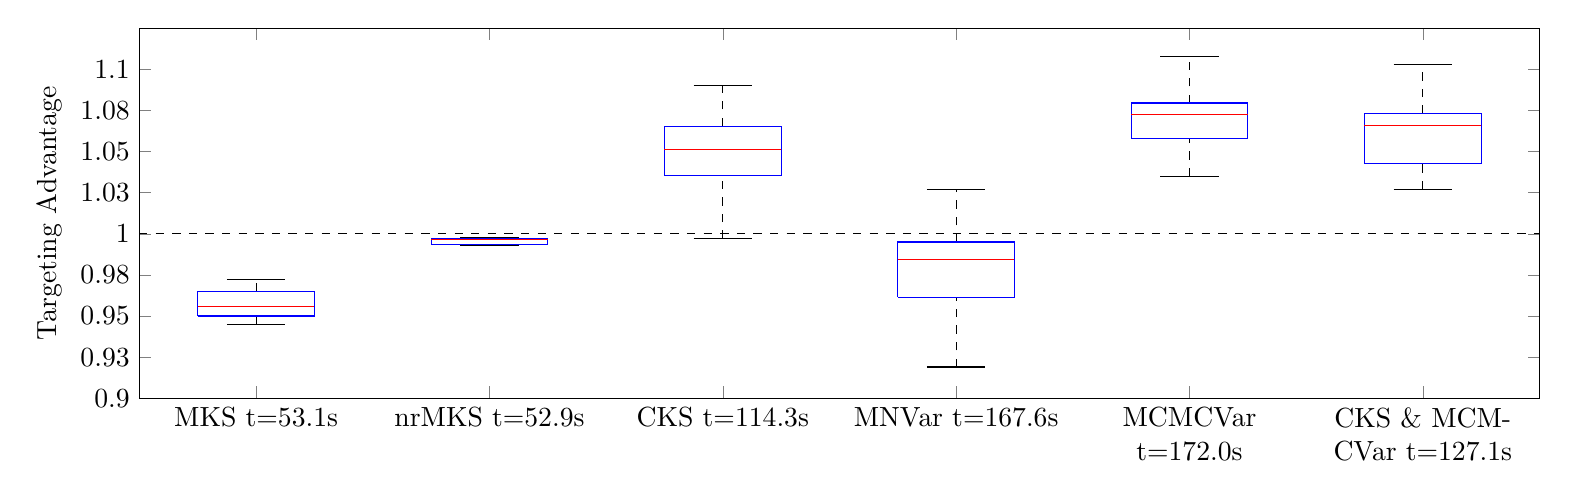
\begin{tikzpicture}

\begin{axis}[%
width=7in,
height=1.85in,
unbounded coords=jump,
scale only axis,
xmin=0.5,
xmax=6.5,
xtick={1, 2, 3, 4, 5, 6,7},%ugliness here
xticklabels={MKS t=53.1s,nrMKS t=52.9s,CKS t=114.3s,MNVar t=167.6s,MCMCVar t=172.0s,CKS \& MCMCVar t=127.1s},%and there
x tick label style={text width=3cm,align=center}, %font=\small,
ymin=0.90,
ymax=1.125,
ytick={.9,.925,.95,.975,1,1.025,1.05,1.075,1.1},
ylabel=Targeting Advantage
]
\addplot [color=black,dashed,forget plot]
  table[row sep=crcr]{1	0.965\\
1	0.972\\
};
\addplot [color=black,dashed,forget plot]
  table[row sep=crcr]{2	0.997\\
2	0.998\\
};
\addplot [color=black,dashed,forget plot]
  table[row sep=crcr]{3	1.0655\\
3	1.09\\
};
\addplot [color=black,dashed,forget plot]
  table[row sep=crcr]{4	0.995\\
4	1.027\\
};
\addplot [color=black,dashed,forget plot]
  table[row sep=crcr]{5	1.0795\\
5	1.108\\
};
\addplot [color=black,dashed,forget plot]
  table[row sep=crcr]{6	1.073\\
6	1.103\\
};
\addplot [color=black,dashed,forget plot]
  table[row sep=crcr]{1	0.945\\
1	0.95\\
};
\addplot [color=black,dashed,forget plot]
  table[row sep=crcr]{2	0.993\\
2	0.9935\\
};
\addplot [color=black,dashed,forget plot]
  table[row sep=crcr]{3	0.997\\
3	1.0355\\
};
\addplot [color=black,dashed,forget plot]
  table[row sep=crcr]{4	0.919\\
4	0.9615\\
};
\addplot [color=black,dashed,forget plot]
  table[row sep=crcr]{5	1.035\\
5	1.058\\
};
\addplot [color=black,dashed,forget plot]
  table[row sep=crcr]{6	1.027\\
6	1.0425\\
};
\addplot [color=black,solid,forget plot]
  table[row sep=crcr]{0.875	0.972\\
1.125	0.972\\
};
\addplot [color=black,solid,forget plot]
  table[row sep=crcr]{1.875	0.998\\
2.125	0.998\\
};
\addplot [color=black,solid,forget plot]
  table[row sep=crcr]{2.875	1.09\\
3.125	1.09\\
};
\addplot [color=black,solid,forget plot]
  table[row sep=crcr]{3.875	1.027\\
4.125	1.027\\
};
\addplot [color=black,solid,forget plot]
  table[row sep=crcr]{4.875	1.108\\
5.125	1.108\\
};
\addplot [color=black,solid,forget plot]
  table[row sep=crcr]{5.875	1.103\\
6.125	1.103\\
};
\addplot [color=black,solid,forget plot]
  table[row sep=crcr]{0.875	0.945\\
1.125	0.945\\
};
\addplot [color=black,solid,forget plot]
  table[row sep=crcr]{1.875	0.993\\
2.125	0.993\\
};
\addplot [color=black,solid,forget plot]
  table[row sep=crcr]{2.875	0.997\\
3.125	0.997\\
};
\addplot [color=black,solid,forget plot]
  table[row sep=crcr]{3.875	0.919\\
4.125	0.919\\
};
\addplot [color=black,solid,forget plot]
  table[row sep=crcr]{4.875	1.035\\
5.125	1.035\\
};
\addplot [color=black,solid,forget plot]
  table[row sep=crcr]{5.875	1.027\\
6.125	1.027\\
};
\addplot [color=blue,solid,forget plot]
  table[row sep=crcr]{0.75	0.95\\
0.75	0.965\\
1.25	0.965\\
1.25	0.95\\
0.75	0.95\\
};
\addplot [color=blue,solid,forget plot]
  table[row sep=crcr]{1.75	0.9935\\
1.75	0.997\\
2.25	0.997\\
2.25	0.9935\\
1.75	0.9935\\
};
\addplot [color=blue,solid,forget plot]
  table[row sep=crcr]{2.75	1.0355\\
2.75	1.0655\\
3.25	1.0655\\
3.25	1.0355\\
2.75	1.0355\\
};
\addplot [color=blue,solid,forget plot]
  table[row sep=crcr]{3.75	0.9615\\
3.75	0.995\\
4.25	0.995\\
4.25	0.9615\\
3.75	0.9615\\
};
\addplot [color=blue,solid,forget plot]
  table[row sep=crcr]{4.75	1.058\\
4.75	1.0795\\
5.25	1.0795\\
5.25	1.058\\
4.75	1.058\\
};
\addplot [color=blue,solid,forget plot]
  table[row sep=crcr]{5.75	1.0425\\
5.75	1.073\\
6.25	1.073\\
6.25	1.0425\\
5.75	1.0425\\
};
\addplot [color=red,solid,forget plot]
  table[row sep=crcr]{0.75	0.956\\
1.25	0.956\\
};
\addplot [color=red,solid,forget plot]
  table[row sep=crcr]{1.75	0.9965\\
2.25	0.9965\\
};
\addplot [color=red,solid,forget plot]
  table[row sep=crcr]{2.75	1.051\\
3.25	1.051\\
};
\addplot [color=red,solid,forget plot]
  table[row sep=crcr]{3.75	0.9845\\
4.25	0.9845\\
};
\addplot [color=red,solid,forget plot]
  table[row sep=crcr]{4.75	1.0725\\
5.25	1.0725\\
};
\addplot [color=red,solid,forget plot]
  table[row sep=crcr]{5.75	1.066\\
6.25	1.066\\
};
\addplot [color=black,dashed,forget plot]
  table[row sep=crcr]{0	1\\
1	1\\
2	1\\
3	1\\
4	1\\
5	1\\
6	1\\
7	1\\
};
\end{axis}
\end{tikzpicture}%}
  \end{center}

  
  \begin{tabular}{p{2.2cm}p{5cm}p{2.2cm}p{5cm}}
  \textbf{MKS:} & Minimum Knowledge Search & \textbf{nrMKS:} & non random MKS \\
  \textbf{CKS:} & Clustered Knowledge Search & \textbf{MNVar:} & Matrix Normal Variance Search \\
  \textbf{MCMCVar:} & Markov Chain Monte Carlo Variance Search & \textbf{CKS \& MCMCvar:} & CKS combined with MCMCVar calculated at 50 sample intervals
  \end{tabular}
  
    Box plot for 20 simulations of active sampling with offline PMF.
  
  t is the time taken for one run of 500 new sample requests.
  
  Values larger than 1 indicate better than random performance.
  
  Lookahead sampling was ignored for computational efficiency reasons.
  
    \caption{Comparison of multiple runs on $80 \times 50$ synthetic data}
    \label{fig:combined_compared}
\end{figure}

Here the performance of all the encountered algorithms so far is evaluated. For fair comparisons it was compared to the average random sampling performance rather than an individual instance(average of random sampling for $80 \times 50$ is found in appendix figure \ref{fig:RandomPMF}). This avoid instances of bad random sampling performance and very good targeted sampling performance creating artificially high values, as in figure \ref{fig:online_pmf_active}.

The first observation to be made is that the proposed MKS algorithm does not perform well, only ensuring close to expected random performance, the non random variation was found to slightly outperform the random variation due to the initial column and row knowledge maximisation (as seen in the knowledge matrix in figure \ref{fig:know_mat_it}).

The CKS search did yield better than random performance nearly consistently, which shows that the targeted approach was successful, though not as well as the more complex MCMCVar one.

Matrix Normal Variance Search (MNVar) did not results in the results found by Sutherland et. al, however this is most likely due to MNVar being sensitive to the parameters used and the parameters found by PMF do not complete empty rows and cells, meaning parameter quality can be very low at the start of the sampling process.

MCMCVar was found to perform best, consistently outdoing random selection, though at the cost of greater complexity. An attempt at reducing complexity while retaining targeting performance is done with the hybrid CKS MCMC algorithm. This resulted in a performance consistently above random sampling and was above to reduce the runtime of 500 sample requests by 27\%. While not very useful for small matrices, as active sampling rarely needs to be done in realtime, this is useful for very large databases such as the Netflix one.


Finally the Max-Min value search mentioned in section \ref{sec:as_goals} was tested but had an average targeting advantage of 0.8 and was only found to be useful to remove some over and under estimation errors, as expected.
% ------------------------------------------------------------------------


%%% Local Variables: 
%%% mode: latex
%%% TeX-master: "../thesis"
%%% End: 

\chapter{Evaluation and Observations}
\ifpdf
    \graphicspath{{Chapter4/Chapter4Figs/PNG/}{Chapter4/Chapter4Figs/PDF/}{Chapter4/Chapter4Figs/}}
\else
    \graphicspath{{Chapter4/Chapter4Figs/EPS/}{Chapter4/Chapter4Figs/}}
\fi

\markboth{\MakeUppercase{\thechapter. Evaluation and Observations}}{\thechapter. Evaluation and Observations}
\section{Test on Larger Datasets}
The final test was to try active sampling on larger and different datasets. For this the movielens dataset \cite{movielensdata}, Drugbank \cite{law2014drugbank} and HIVA \cite{hivadata} were used.
\subsection{Pre-Processing}
Most of the time the datasets came in various formats that had to be cleaned up and converted to matlab format. Additionally the movielens dataset had many incomplete entries (unrated movies). This meant creating a subset as non-sparse as possible to split up into useful test, validation and training sets. For the other datasets the data was split into respective training,test and validation sets, with an initial training set of about 2.5 \%.


\subsection{Dealing with large sizes}

The main challenge with using large datasets is the time taken, especially due to scaling up with the complexity of datasets. For this reason data was often reduced to manageable datasets and process in batches for training. This is advantageous when algorithms are bounded by $O(MN)$, $O(M^2N^2)$ and higher orders as halving data results in $O(\left(\frac{M}{2}\right)^2 \left(\frac{N}{2}\right)^2)+ O(\left(\frac{M}{2}\right)^2 \left(\frac{N}{2}\right)^2) = \frac{1}{8}O(M^2 N^2)$, which results in an improvement of nearly a factor of 10 for splitting it into two equal sets. For more datasets and high complexities this is even more interesting. The main disadvantage is that by reducing the data available to PMF and other algorithms in one batch that the model quality can be reduced. For this reason it was ensured that each batch have roughly $5000$ entries or more. This is a variant of the batch splitting that appears in the code published by Ruslan Salakhutdinov\cite{SalMnih2008} \footnote{\url{http://www.cs.toronto.edu/~rsalakhu/BPMF.html}}.
\subsection{Results}

\begin{figure}[!htbp]
  \begin{center}
    \resizebox{\textwidth}{!}{% This file was created by matlab2tikz v0.4.7 running on MATLAB 8.1.
% Copyright (c) 2008--2014, Nico Schlömer <nico.schloemer@gmail.com>
% All rights reserved.
% Minimal pgfplots version: 1.3
% 
% The latest updates can be retrieved from
%   http://www.mathworks.com/matlabcentral/fileexchange/22022-matlab2tikz
% where you can also make suggestions and rate matlab2tikz.
% 
\begin{tikzpicture}

\begin{axis}[%
width=2in,
height=2in,
axis on top,
scale only axis,
xmin=0.5,
xmax=515.5,
y dir=reverse,
ymin=0.5,
ymax=443.5,
name=plot2,
title={Random Request}
]
\addplot [forget plot] graphics [xmin=0.5,xmax=515.5,ymin=0.5,ymax=443.5] {movielens_full_mks-1.png};
\end{axis}

\begin{axis}[%
width=2in,
height=2in,
scale only axis,
xmin=0,
xmax=60,
ymin=0.5,
ymax=1,
ylabel={RMSE},
at=(plot2.left of south west),
anchor=right of south east,
title={Target Advantage:1.036},
legend style={at={(0.142803670610963,0.726939714277153)},anchor=south west,draw=black,fill=white,legend cell align=left}
]
\addplot [color=blue,solid]
  table[row sep=crcr]{1	0.982028046935178\\
2	0.981313847284314\\
3	0.980122834205141\\
4	0.980376744775176\\
5	0.979389858496978\\
6	0.980768893333339\\
7	0.980753479092152\\
8	0.980999432205153\\
9	0.981062593899508\\
10	0.980786948804123\\
11	0.980322903462218\\
12	0.97995450146891\\
13	0.979718111738063\\
14	0.979674421720633\\
15	0.979617209105709\\
16	0.979511809092559\\
17	0.979262807576767\\
18	0.979431897970538\\
19	0.979686035446558\\
20	0.979792911478351\\
21	0.978862616690479\\
22	0.978500604597058\\
23	0.978661511571657\\
24	0.97958028684088\\
25	0.978988157087365\\
26	0.979469147108749\\
27	0.979270929555654\\
28	0.979686075954478\\
29	0.979796501218589\\
30	0.979624612822433\\
31	0.98025669770191\\
32	0.979678467637759\\
33	0.978895553572444\\
34	0.979263159621612\\
35	0.979297130059643\\
36	0.979493063587379\\
37	0.97843109950656\\
38	0.976698288793067\\
39	0.973863899977724\\
40	0.971635293729348\\
41	0.96941635760875\\
42	0.965627489693154\\
43	0.96363913180515\\
44	0.962452152728478\\
45	0.9591732572088\\
46	0.952665582064301\\
47	0.951210405453268\\
48	0.946018508335472\\
49	0.943605911774556\\
50	0.940301621809507\\
51	0.935668521887269\\
52	0.939507093880165\\
53	0.932638029819088\\
54	0.933202528007017\\
55	0.9295501475103071\\
56	0.921986882000124\\
57	0.91800330237417\\
58	0.909023046892924\\
59	0.89156828622473\\
60	0.890785973072127\\
};
\addlegendentry{Random};

\addplot [color=black!50!green,solid]
  table[row sep=crcr]{1	0.970647651181982\\
2	0.981840888142382\\
3	0.981803933849183\\
4	0.982679424012043\\
5	0.982697357936221\\
6	0.982227862310657\\
7	0.982398625675358\\
8	0.981591863878341\\
9	0.980638743394689\\
10	0.981547249504257\\
11	0.981089358442673\\
12	0.980189414590985\\
13	0.979645170101084\\
14	0.979000082648651\\
15	0.97788637770358\\
16	0.977710799016321\\
17	0.976876287732414\\
18	0.976248991706231\\
19	0.975556094688078\\
20	0.974368466783688\\
21	0.973137866383247\\
22	0.972434350677177\\
23	0.971758115213478\\
24	0.969799473193526\\
25	0.969710472975677\\
26	0.969802155234243\\
27	0.968735886309691\\
28	0.968258785161049\\
29	0.96832148606297\\
30	0.967477285971869\\
31	0.966059705330264\\
32	0.96469080918169\\
33	0.962404386483437\\
34	0.96134784603003\\
35	0.960192336171133\\
36	0.95966227706608\\
37	0.958107408117533\\
38	0.956562363782058\\
39	0.955321060038214\\
40	0.944022873685131\\
41	0.952207549182605\\
42	0.939577587105911\\
43	0.938203495418684\\
44	0.926281810517993\\
45	0.924307301448261\\
46	0.913455063414406\\
47	0.911529372965638\\
48	0.908506423289442\\
49	0.90531894492551\\
50	0.891055623806149\\
51	0.886107203867645\\
52	0.899414049462608\\
53	0.870659367141099\\
54	0.8633611505573\\
55	0.865912508823454\\
56	0.852119968688436\\
57	0.836650679697913\\
58	0.824576707166225\\
59	0.814564920411805\\
60	0.814095354263708\\
};
\addlegendentry{Targeted};

\end{axis}

\begin{axis}[%
width=2in,
height=2in,
axis on top,
scale only axis,
xmin=0.5,
xmax=515.5,
y dir=reverse,
ymin=0.5,
ymax=443.5,
at=(plot2.right of south east),
anchor=left of south west,
title={Active Request}
]
\addplot [forget plot] graphics [xmin=0.5,xmax=515.5,ymin=0.5,ymax=443.5] {movielens_full_mks-2.png};
\end{axis}
\end{tikzpicture}%}
  	\textbf{MKS}
  \end{center}
  
  \begin{center}
    \resizebox{\textwidth}{!}{% This file was created by matlab2tikz v0.4.7 running on MATLAB 8.1.
% Copyright (c) 2008--2014, Nico Schlömer <nico.schloemer@gmail.com>
% All rights reserved.
% Minimal pgfplots version: 1.3
% 
% The latest updates can be retrieved from
%   http://www.mathworks.com/matlabcentral/fileexchange/22022-matlab2tikz
% where you can also make suggestions and rate matlab2tikz.
% 
\begin{tikzpicture}

\begin{axis}[%
width=2in,
height=2in,
axis on top,
scale only axis,
xmin=0.5,
xmax=515.5,
y dir=reverse,
ymin=0.5,
ymax=443.5,
name=plot2,
title={Random Request}
]
\addplot [forget plot] graphics [xmin=0.5,xmax=515.5,ymin=0.5,ymax=443.5] {movielens_full_mcmcvar-1.png};
\end{axis}

\begin{axis}[%
width=2in,
height=2in,
scale only axis,
xmin=0,
xmax=60,
ymin=0.5,
ymax=1,
ylabel={RMSE},
name=plot1,
at=(plot2.left of south west),
anchor=right of south east,
title={Target Advantage:1.094},
legend style={at={(0.137108164753053,0.598145377590488)},anchor=south west,draw=black,fill=white,legend cell align=left}
]
\addplot [color=blue,solid]
  table[row sep=crcr]{1	0.984852598373419\\
2	0.98691197114624\\
3	0.991102916409731\\
4	0.989101045253396\\
5	0.990274605940381\\
6	0.989587056411546\\
7	0.989682882893472\\
8	0.990838413768203\\
9	0.989713262684312\\
10	0.989113014658497\\
11	0.988784512058675\\
12	0.988516194961599\\
13	0.987287554463471\\
14	0.986337870690433\\
15	0.985603461818197\\
16	0.985586116422425\\
17	0.985127139707444\\
18	0.98458225014603\\
19	0.984066671341418\\
20	0.984049302438737\\
21	0.984253082695877\\
22	0.984209042402069\\
23	0.984499487432097\\
24	0.984431761218986\\
25	0.984418318245746\\
26	0.984420095564841\\
27	0.983962998861527\\
28	0.983621799088022\\
29	0.982765879514971\\
30	0.982733719064244\\
31	0.984167522109069\\
32	0.983741593983587\\
33	0.974887369453717\\
34	0.975466388653259\\
35	0.976177289831995\\
36	0.97672895276212\\
37	0.977140763032278\\
38	0.977496188147104\\
39	0.976908479938175\\
40	0.977358043875656\\
41	0.976977285457701\\
42	0.976372694481213\\
43	0.97659170605498\\
44	0.975696574578324\\
45	0.973777926273301\\
46	0.964773433765611\\
47	0.964600538710833\\
48	0.961304280477245\\
49	0.960795227647529\\
50	0.9609653553643494\\
51	0.9509037568851852\\
52	0.9508308171499821\\
53	0.9508955748504522\\
54	0.9505497720121432\\
55	0.94030272969043\\
56	0.947518677263209\\
57	0.942474651608353\\
58	0.93956529877619\\
59	0.934668518407651\\
60	0.928990531399978\\
};
\addlegendentry{Random};

\addplot [color=black!50!green,solid]
  table[row sep=crcr]{1	0.988165263625116\\
2	0.97072080088941\\
3	0.967925457816392\\
4	0.966185861064171\\
5	0.965911128878419\\
6	0.965970342420003\\
7	0.964358662199566\\
8	0.962814178844116\\
9	0.960431756057359\\
10	0.958033325707069\\
11	0.955062802073348\\
12	0.952068151961177\\
13	0.949416421294012\\
14	0.946080864196191\\
15	0.943059425083887\\
16	0.939767154794794\\
17	0.936981834582013\\
18	0.934574522932126\\
19	0.932062174718115\\
20	0.929989181248392\\
21	0.928022225056826\\
22	0.925425721658326\\
23	0.922515471521346\\
24	0.919426734120754\\
25	0.916445283037594\\
26	0.913549071853868\\
27	0.910767015392709\\
28	0.907644469299417\\
29	0.90471704042181\\
30	0.901824334452771\\
31	0.898877513488215\\
32	0.896404744967885\\
33	0.893838322761032\\
34	0.890722664282112\\
35	0.887443116440602\\
36	0.884700355396298\\
37	0.881689799019854\\
38	0.879313992714304\\
39	0.877594887703434\\
40	0.87565701075817\\
41	0.874756825275093\\
42	0.873865170823171\\
43	0.872829685081365\\
44	0.872908392754685\\
45	0.871104854494587\\
46	0.869485529662145\\
47	0.86532648067117\\
48	0.856438552267593\\
49	0.852866011449603\\
50	0.85049353314237\\
51	0.847972308837873\\
52	0.845603315546848\\
53	0.842987801014843\\
54	0.840631326715836\\
55	0.837045880920788\\
56	0.836129812560303\\
57	0.835775064772113\\
58	0.831313544523637\\
59	0.819074491394663\\
60	0.81568314654427\\
};
\addlegendentry{Targeted};

\end{axis}

\begin{axis}[%
width=2in,
height=2in,
axis on top,
scale only axis,
xmin=0.5,
xmax=515.5,
y dir=reverse,
ymin=0.5,
ymax=443.5,
name=plot4,
at=(plot1.below south west),
anchor=above north west,
title={Original (Incomplete)}
]
\addplot [forget plot] graphics [xmin=0.5,xmax=515.5,ymin=0.5,ymax=443.5] {movielens_full_mcmcvar-2.png};
\end{axis}

\begin{axis}[%
width=2in,
height=2in,
axis on top,
scale only axis,
xmin=0.5,
xmax=515.5,
y dir=reverse,
ymin=0.5,
ymax=443.5,
name=plot5,
at=(plot4.right of south east),
anchor=left of south west,
title={Active Request}
]
\addplot [forget plot] graphics [xmin=0.5,xmax=515.5,ymin=0.5,ymax=443.5] {movielens_full_mcmcvar-3.png};
\end{axis}

\begin{axis}[%
width=2in,
height=2in,
axis on top,
scale only axis,
xmin=0.5,
xmax=515.5,
y dir=reverse,
ymin=0.5,
ymax=443.5,
name=plot6,
at=(plot5.right of south east),
anchor=left of south west,
title={Targeted Prediction}
]
\addplot [forget plot] graphics [xmin=0.5,xmax=515.5,ymin=0.5,ymax=443.5] {movielens_full_mcmcvar-4.png};
\end{axis}

\begin{axis}[%
width=2in,
height=2in,
axis on top,
scale only axis,
xmin=0.5,
xmax=515.5,
y dir=reverse,
ymin=0.5,
ymax=443.5,
at=(plot6.above north west),
anchor=below south west,
title={Random Prediction}
]
\addplot [forget plot] graphics [xmin=0.5,xmax=515.5,ymin=0.5,ymax=443.5] {movielens_full_mcmcvar-5.png};
\end{axis}
\end{tikzpicture}%}
    \textbf{MCMCVar}
  \end{center}
  
  
   Each iteration represents adding a batch of 50 samples based on the selection criteria.
  
  The predictor used was PMF with $20$ features, $\lambda = 0.01$ and $\mu = 0.005$.
  
  The Active and Random request matrix may be better seen in colour.
    
    \caption{MovieLens Dataset Active Sampling Test on $443\times 515$ subgroup batch}
    \label{fig:movielens_full_mcmcvar}
\end{figure}


\begin{table}[H]
  \begin{center}
\begin{tabular}{l|l|l|l|}
&	\textbf{CKS}	& \textbf{MCMCVar} & \textbf{CKS MCMCVar Comb} \\ \hline
Targeting Advantage	& 1.036 &	1.094 &	1.073 \\ \hline
Time (hours) &	1.677 &	2.083	&1.833 \\ \hline
Time/sample (s)	& 2	& 2.5 &	2.2 \\ \hline
\end{tabular}
\end{center}
\caption{Active Sampling Results on MovieLens Dataset}
\label{table:movielens_res}
\end{table}


Figure \ref{fig:movielens_full_mcmcvar} and table \ref{table:movielens_res} show the sampling performance on the MovieLens database. This database is very similar in nature to the synthetic one, having discrete values ranging from 1 to 5. However as MovieLens is a "real" database the values are more concentrated around 3, due to users often being and rating a film 3 stars. This explains the better RMSE performance on a set of similar values. The prediction matrices visually show the average rating being closer to 3 (yellow and green representing 3 and 4). Due to time only one run was done for each algorithm and dataset. The performance of the CKS MCMCVar is, as expected, in between CKS and MCMVar in targeting advantage but its runtime is slightly better than the MCMCVar.

\begin{figure}[!htbp]
  \begin{center}
    \resizebox{\textwidth}{!}{% This file was created by matlab2tikz v0.4.7 running on MATLAB 8.1.
% Copyright (c) 2008--2014, Nico Schlömer <nico.schloemer@gmail.com>
% All rights reserved.
% Minimal pgfplots version: 1.3
% 
% The latest updates can be retrieved from
%   http://www.mathworks.com/matlabcentral/fileexchange/22022-matlab2tikz
% where you can also make suggestions and rate matlab2tikz.
% 
\begin{tikzpicture}

\begin{axis}[%
width=1.9in,
height=2in,
axis on top,
scale only axis,
xmin=0.5,
xmax=425.5,
y dir=reverse,
ymin=0.5,
ymax=94.5,
name=plot2,
title={Random Request}
]
\addplot [forget plot] graphics [xmin=0.5,xmax=425.5,ymin=0.5,ymax=94.5] {drugbank_mks-1.png};
\end{axis}

\begin{axis}[%
width=2in,
height=2in,
scale only axis,
xmin=0,
xmax=200,
ymin=0.17,
ymax=0.2,
ylabel={RMSE},
name=plot1,
at=(plot2.left of south west),
anchor=right of south east,
title={Target Advantage:1.087},
legend style={draw=black,fill=white,legend cell align=left}
]
\addplot [color=blue,solid]
  table[row sep=crcr]{1	0.196826613374851\\
2	0.196822102699619\\
3	0.196817574879202\\
4	0.196761558589051\\
5	0.196720244989688\\
6	0.196698751583184\\
7	0.196693559103845\\
8	0.196703041325511\\
9	0.19673067818992\\
10	0.196770820790956\\
11	0.196809506972088\\
12	0.196866318503207\\
13	0.196916391297849\\
14	0.196958496343147\\
15	0.196976375516096\\
16	0.196987091298918\\
17	0.196997816444646\\
18	0.197011123355403\\
19	0.197027018752967\\
20	0.197045509385881\\
21	0.197071471710442\\
22	0.197097562647291\\
23	0.197128765173989\\
24	0.197162598110185\\
25	0.197196569483331\\
26	0.197235683993435\\
27	0.19726974369708\\
28	0.197303943232123\\
29	0.197338283212181\\
30	0.197377887837708\\
31	0.197415122774613\\
32	0.197449887805815\\
33	0.197479654999463\\
34	0.197512084404899\\
35	0.197547183107262\\
36	0.197582523674699\\
37	0.19761810712476\\
38	0.197646035196942\\
39	0.197679177020605\\
40	0.197712463249597\\
41	0.197743149927921\\
42	0.197776427845599\\
43	0.197814958980522\\
44	0.197863785520986\\
45	0.19791277586521\\
46	0.197964499277688\\
47	0.198011056385056\\
48	0.198057776104965\\
49	0.198101984199233\\
50	0.198146255132022\\
51	0.19818531986928\\
52	0.198219162383117\\
53	0.19824776656877\\
54	0.198276515404854\\
55	0.19829729972817\\
56	0.198320711818997\\
57	0.198344263735553\\
58	0.198367956149309\\
59	0.198386461218061\\
60	0.198402378415963\\
61	0.198421043918599\\
62	0.198442465332166\\
63	0.198461292824381\\
64	0.198480258171749\\
65	0.198496733955091\\
66	0.198505224356023\\
67	0.198519109309821\\
68	0.19853037432523\\
69	0.198536252886381\\
70	0.198539251234753\\
71	0.198545021126881\\
72	0.19854536800334\\
73	0.198545711718606\\
74	0.198546175756878\\
75	0.198543973392917\\
76	0.198547223684329\\
77	0.198550599093741\\
78	0.198551176737141\\
79	0.198551751883633\\
80	0.198557817788559\\
81	0.198563765960484\\
82	0.198572414808899\\
83	0.198572725696378\\
84	0.198569944637143\\
85	0.198572829268228\\
86	0.198573001434707\\
87	0.198570453652211\\
88	0.198570747263772\\
89	0.198565327523754\\
90	0.198554305454512\\
91	0.198537662727755\\
92	0.19852673179857\\
93	0.198513040299136\\
94	0.198493699962227\\
95	0.198474183711422\\
96	0.19844898789189\\
97	0.198423746475729\\
98	0.198401218795048\\
99	0.198381272257069\\
100	0.198358517440467\\
101	0.198341413790304\\
102	0.198327199213941\\
103	0.19830724539179\\
104	0.198287253802189\\
105	0.198267369425171\\
106	0.198250532462076\\
107	0.198236463124996\\
108	0.198219416460174\\
109	0.198205435866955\\
110	0.198188323216662\\
111	0.198171177385281\\
112	0.198156676058176\\
113	0.198153617907412\\
114	0.198141893415235\\
115	0.198130144068725\\
116	0.198121361565256\\
117	0.198112705291531\\
118	0.198112738980752\\
119	0.198115629284568\\
120	0.198124395618289\\
121	0.198130441380415\\
122	0.198139509374007\\
123	0.198154489409684\\
124	0.198166324046653\\
125	0.198187130374285\\
126	0.198211002768375\\
127	0.198231870968079\\
128	0.198258724681868\\
129	0.198285619862936\\
130	0.198306581547669\\
131	0.198324652488388\\
132	0.198345676952225\\
133	0.198369805988217\\
134	0.198247960550521\\
135	0.198250997111752\\
136	0.19818248708571\\
137	0.198197767173026\\
138	0.198200955607289\\
139	0.198213171821764\\
140	0.198212937084605\\
141	0.198234393686785\\
142	0.198227881697908\\
143	0.198240013441828\\
144	0.198179600217567\\
145	0.198042594916363\\
146	0.198010882406586\\
147	0.198023535123459\\
148	0.197899093795251\\
149	0.197624575663976\\
150	0.197353131995106\\
151	0.197344093863371\\
152	0.197338382736218\\
153	0.197232655223357\\
154	0.196973011107666\\
155	0.19696101821541\\
156	0.196851852458083\\
157	0.196742692615299\\
158	0.196727398986962\\
159	0.196488667019868\\
160	0.196447203656828\\
161	0.196140181671912\\
162	0.195933825469556\\
163	0.195816396783929\\
164	0.195816505787085\\
165	0.195488185674253\\
166	0.195174743730206\\
167	0.195095982240107\\
168	0.194811839255991\\
169	0.194758720480649\\
170	0.194545737514367\\
171	0.19413605851022\\
172	0.193931628442677\\
173	0.193448723190485\\
174	0.193355366924184\\
175	0.193035065207151\\
176	0.192563935434621\\
177	0.192193075777004\\
178	0.19237371878947\\
179	0.1921922131758\\
180	0.191690229695904\\
181	0.191242296530849\\
182	0.190727786839977\\
183	0.19055356600314\\
184	0.190167330542975\\
185	0.190144555660148\\
186	0.189846649553177\\
187	0.189628661574737\\
188	0.189184265751363\\
189	0.188679864277698\\
190	0.188554026362073\\
191	0.188050784130347\\
192	0.18781833625948\\
193	0.187258310096698\\
194	0.186971777023232\\
195	0.18666826521095\\
196	0.186043013903858\\
197	0.185610781968886\\
198	0.18499715618931\\
199	0.18454253590226\\
200	0.184277218173401\\
201	0.184022491999213\\
202	0.184080132539489\\
203	0.183911057085701\\
204	0.1835686817632\\
205	0.183292775423172\\
206	0.183067904714137\\
207	0.182421149209129\\
208	0.182196115587564\\
209	0.181989028686077\\
210	0.18166802114925\\
211	0.181509890929687\\
212	0.181133054919555\\
213	0.180356320996808\\
214	0.179920777509649\\
215	0.179493011086263\\
216	0.179307949309784\\
217	0.179196710810504\\
218	0.179176960797155\\
219	0.179318409134389\\
220	0.179405651787231\\
221	0.178270128818522\\
222	0.17711796476038\\
223	0.177086612176444\\
224	0.176582650998019\\
225	0.175873950321181\\
};
\addlegendentry{Random};

\addplot [color=black!50!green,solid]
  table[row sep=crcr]{1	0.197040904797464\\
2	0.196462811149669\\
3	0.195851231725299\\
4	0.195293277678862\\
5	0.194791598210471\\
6	0.194381300442572\\
7	0.194059600560926\\
8	0.193795833517265\\
9	0.193582567135794\\
10	0.19341568447315\\
11	0.193299847989704\\
12	0.193221831986144\\
13	0.193169610519167\\
14	0.193129100190812\\
15	0.193110987651204\\
16	0.192969110812937\\
17	0.19284151261242\\
18	0.192738811913731\\
19	0.192660998806151\\
20	0.192603077395144\\
21	0.192546918169808\\
22	0.19251084480818\\
23	0.192490137440965\\
24	0.192492483607916\\
25	0.1924973669815\\
26	0.192517785003874\\
27	0.192540982651496\\
28	0.192550429292241\\
29	0.192543662713942\\
30	0.192458501459227\\
31	0.192378640227559\\
32	0.192212942390482\\
33	0.191749245053611\\
34	0.19127667690014\\
35	0.190803961665683\\
36	0.19033629129958\\
37	0.189868477859292\\
38	0.189394676831176\\
39	0.188923331663032\\
40	0.188454447293291\\
41	0.187990638639604\\
42	0.187529303647002\\
43	0.187067831483955\\
44	0.186606222308561\\
45	0.186149716642148\\
46	0.185703578961191\\
47	0.185257316331325\\
48	0.184813560613639\\
49	0.184374952620082\\
50	0.183942905049668\\
51	0.183516040757722\\
52	0.183089066850155\\
53	0.182659019713132\\
54	0.182234174212943\\
55	0.18180922146276\\
56	0.181384161711342\\
57	0.1809853843799\\
58	0.180610660031967\\
59	0.180308092097561\\
60	0.179817517126109\\
61	0.179425684265793\\
62	0.179334435979491\\
63	0.179252057608618\\
64	0.179166736655358\\
65	0.179081561215866\\
66	0.178996532119222\\
67	0.178858348544689\\
68	0.178720270488338\\
69	0.178582298692932\\
70	0.178444433906061\\
71	0.178306676880179\\
72	0.178165886843355\\
73	0.178009458795251\\
74	0.17785312566294\\
75	0.177633392254874\\
76	0.177413704208152\\
77	0.177194062145256\\
78	0.176974466693155\\
79	0.176766732349196\\
80	0.176559055011474\\
81	0.176351435341829\\
82	0.176146837857645\\
83	0.17593908847869\\
84	0.175731398471757\\
85	0.175523768516772\\
86	0.175319173801719\\
87	0.175114642836455\\
88	0.174919122325476\\
89	0.174911666676811\\
90	0.174904431450215\\
91	0.174890943916933\\
92	0.174874431455623\\
93	0.174789392451511\\
94	0.174688053551284\\
95	0.174586861667323\\
96	0.174544964018471\\
97	0.174503262156179\\
98	0.174455138605194\\
99	0.174317055193845\\
100	0.174179089810199\\
101	0.174044384840253\\
102	0.17392554690919\\
103	0.17380684472564\\
104	0.173745014054144\\
105	0.173673201612893\\
106	0.173601564527195\\
107	0.173530103813818\\
108	0.173455419771335\\
109	0.173380911268396\\
110	0.173306579334426\\
111	0.173194791585304\\
112	0.173072607356118\\
113	0.172950561500483\\
114	0.172828654968704\\
115	0.172699980843077\\
116	0.172564520119882\\
117	0.172429189706569\\
118	0.172290520579724\\
119	0.172134585150534\\
120	0.171981750368481\\
121	0.171832276118338\\
122	0.171754755731733\\
123	0.17169387731927\\
124	0.171633196011374\\
125	0.171572712948092\\
126	0.171512429277052\\
127	0.171455452990175\\
128	0.171488833067868\\
129	0.171522493837984\\
130	0.171552913645373\\
131	0.171583613795173\\
132	0.171611064327347\\
133	0.171642019359082\\
134	0.171683423017329\\
135	0.171725120615985\\
136	0.171760015271966\\
137	0.171798601153553\\
138	0.171833923189341\\
139	0.171869538325651\\
140	0.171943081439812\\
141	0.172030708907528\\
142	0.172118677815597\\
143	0.172206989762314\\
144	0.172302554230603\\
145	0.172405392806161\\
146	0.172508591180404\\
147	0.172612031226866\\
148	0.172718836048082\\
149	0.172829495661083\\
150	0.172940526511678\\
151	0.173051930322664\\
152	0.173156472690076\\
153	0.173257760203558\\
154	0.173359415925858\\
155	0.17346144159656\\
156	0.173567350645208\\
157	0.173673636234808\\
158	0.17378030014691\\
159	0.173890867203366\\
160	0.17400181928605\\
161	0.174116689562491\\
162	0.174235488217303\\
163	0.174354683674878\\
164	0.174470613799297\\
165	0.174594039377666\\
166	0.174706844315389\\
167	0.174823604816612\\
168	0.17494076729558\\
169	0.175058333677691\\
170	0.175168916274258\\
171	0.175276197969298\\
172	0.175383878872847\\
173	0.175491960931405\\
174	0.175596731580467\\
175	0.175701903766164\\
176	0.175811069229709\\
177	0.175935037079098\\
178	0.176040750760928\\
179	0.176146872393365\\
180	0.176242148055213\\
181	0.176345060979796\\
182	0.176452008339961\\
183	0.176559370860293\\
184	0.176667150613606\\
185	0.176748876777892\\
186	0.176827203613559\\
187	0.176894514342966\\
188	0.176958398030437\\
189	0.177022664760056\\
190	0.177087316558814\\
191	0.177152355467878\\
192	0.177217783542724\\
193	0.177287266866235\\
194	0.177357146946226\\
195	0.177438451881841\\
196	0.177520168186242\\
197	0.177602298027508\\
198	0.177684843588991\\
199	0.177775196696181\\
200	0.177869678630166\\
201	0.177964593474562\\
202	0.178056075857102\\
203	0.178151706336315\\
204	0.178247776235015\\
205	0.178344287876214\\
206	0.178441243599465\\
207	0.178549541930615\\
208	0.178658299124328\\
209	0.178778773541559\\
210	0.178899722557366\\
211	0.179017238099121\\
212	0.179099712190035\\
213	0.179233481508054\\
214	0.179398698079732\\
215	0.179567465111378\\
216	0.179734874443929\\
217	0.179900201915498\\
218	0.180062334384037\\
219	0.180219470467316\\
220	0.180368494816472\\
221	0.180515980508468\\
222	0.180660031930373\\
223	0.180773234355741\\
224	0.180942928124375\\
225	0.181052896045912\\
};
\addlegendentry{Targeted};

\end{axis}

\begin{axis}[%
width=2in,
height=2in,
axis on top,
scale only axis,
xmin=0.5,
xmax=425.5,
y dir=reverse,
ymin=0.5,
ymax=94.5,
name=plot4,
at=(plot1.below south west),
anchor=above north west,
title={Original}
]
\addplot [forget plot] graphics [xmin=0.5,xmax=425.5,ymin=0.5,ymax=94.5] {drugbank_mks-2.png};
\end{axis}

\begin{axis}[%
width=2in,
height=2in,
axis on top,
scale only axis,
xmin=0.5,
xmax=425.5,
y dir=reverse,
ymin=0.5,
ymax=94.5,
name=plot5,
at=(plot4.right of south east),
anchor=left of south west,
title={Active Request}
]
\addplot [forget plot] graphics [xmin=0.5,xmax=425.5,ymin=0.5,ymax=94.5] {drugbank_mks-3.png};
\end{axis}

\begin{axis}[%
width=2in,
height=2in,
axis on top,
scale only axis,
xmin=0.5,
xmax=425.5,
y dir=reverse,
ymin=0.5,
ymax=94.5,
name=plot6,
at=(plot5.right of south east),
anchor=left of south west,
title={Targeted Prediction}
]
\addplot [forget plot] graphics [xmin=0.5,xmax=425.5,ymin=0.5,ymax=94.5] {drugbank_mks-4.png};
\end{axis}

\begin{axis}[%
width=2in,
height=2in,
axis on top,
scale only axis,
xmin=0.5,
xmax=425.5,
y dir=reverse,
ymin=0.5,
ymax=94.5,
at=(plot6.above north west),
anchor=below south west,
title={Random Prediction}
]
\addplot [forget plot] graphics [xmin=0.5,xmax=425.5,ymin=0.5,ymax=94.5] {drugbank_mks-5.png};
\end{axis}
\end{tikzpicture}%}
  	\textbf{MKS}
  \end{center}
  
  \begin{center}
    \resizebox{\textwidth}{!}{% This file was created by matlab2tikz v0.4.7 running on MATLAB 8.1.
% Copyright (c) 2008--2014, Nico Schlömer <nico.schloemer@gmail.com>
% All rights reserved.
% Minimal pgfplots version: 1.3
% 
% The latest updates can be retrieved from
%   http://www.mathworks.com/matlabcentral/fileexchange/22022-matlab2tikz
% where you can also make suggestions and rate matlab2tikz.
% 
\begin{tikzpicture}

\begin{axis}[%
width=2in,
height=2in,
axis on top,
scale only axis,
xmin=0.5,
xmax=425.5,
y dir=reverse,
ymin=0.5,
ymax=94.5,
name=plot2,
title={Random Prediction}
]
\addplot [forget plot] graphics [xmin=0.5,xmax=425.5,ymin=0.5,ymax=94.5] {drugbank_mcmcvar-1.png};
\end{axis}

\begin{axis}[%
width=2in,
height=2in,
scale only axis,
xmin=0,
xmax=200,
ymin=0.15,
ymax=0.2,
ylabel={RMSE},
at=(plot2.left of south west),
anchor=right of south east,
title={Target Advantage:1.046},
legend style={draw=black,fill=white,legend cell align=left}
]
\addplot [color=blue,solid]
  table[row sep=crcr]{1	0.196828861786541\\
2	0.196826586614039\\
3	0.196738379453101\\
4	0.196719700543625\\
5	0.19671625506598\\
6	0.196732821772271\\
7	0.196754665705918\\
8	0.196774895197594\\
9	0.196806820358533\\
10	0.196842979101301\\
11	0.196864974431028\\
12	0.196873330069914\\
13	0.196888703917345\\
14	0.196906866148586\\
15	0.196929758666602\\
16	0.196947553305973\\
17	0.196965404014791\\
18	0.196988198602187\\
19	0.197018459197057\\
20	0.197043712651269\\
21	0.19706902510502\\
22	0.197094354368864\\
23	0.197117180734676\\
24	0.197135021393787\\
25	0.197152918722577\\
26	0.197165774186535\\
27	0.197176155691951\\
28	0.197186543209574\\
29	0.197196936745953\\
30	0.197207384672082\\
31	0.197217887101094\\
32	0.19722590773392\\
33	0.197228904669068\\
34	0.19723190232918\\
35	0.197239936144656\\
36	0.197250518260902\\
37	0.197263555774243\\
38	0.197276649262941\\
39	0.197287250256814\\
40	0.197300408029\\
41	0.197308518326929\\
42	0.197319187377387\\
43	0.197327356795462\\
44	0.197335580946999\\
45	0.197338742954447\\
46	0.197339397173823\\
47	0.197342613289367\\
48	0.197343318963413\\
49	0.197343917171263\\
50	0.197341998352463\\
51	0.197342648113291\\
52	0.197343243389467\\
53	0.19734636018922\\
54	0.197344375356862\\
55	0.197350021016533\\
56	0.197355669387135\\
57	0.197363903422449\\
58	0.197369557220509\\
59	0.19737267916156\\
60	0.197373266463948\\
61	0.197376443468392\\
62	0.197384752307273\\
63	0.197395658535737\\
64	0.197404028499238\\
65	0.197409859403403\\
66	0.197418239049235\\
67	0.197424075886746\\
68	0.197429915694513\\
69	0.19743581139574\\
70	0.197444262510686\\
71	0.197450164322894\\
72	0.197458677498402\\
73	0.197459417073547\\
74	0.197462714813585\\
75	0.197466013638593\\
76	0.197466750766865\\
77	0.197464866852164\\
78	0.197470736494038\\
79	0.197479232331047\\
80	0.197487785954753\\
81	0.197496291789582\\
82	0.197507430816656\\
83	0.197515893601909\\
84	0.197521781259257\\
85	0.197527671927585\\
86	0.197530982657378\\
87	0.197539518616713\\
88	0.197550699876034\\
89	0.197561888204076\\
90	0.197567848584798\\
91	0.197571220398038\\
92	0.197572000734888\\
93	0.197572780281983\\
94	0.197573559036041\\
95	0.197574336993764\\
96	0.197575114151846\\
97	0.197578549088828\\
98	0.197582041473666\\
99	0.197588195798738\\
100	0.197594353509273\\
101	0.197595241582803\\
102	0.197601350570017\\
103	0.197607462867226\\
104	0.197616249391527\\
105	0.197625041302358\\
106	0.197639132836296\\
107	0.197653286659347\\
108	0.197667502907424\\
109	0.197673747291371\\
110	0.197682621362508\\
111	0.197691556120107\\
112	0.197705757873831\\
113	0.197719969252003\\
114	0.19773687884999\\
115	0.197753800196113\\
116	0.197768094044686\\
117	0.197779757391943\\
118	0.197791428487773\\
119	0.197805751651922\\
120	0.197822784765804\\
121	0.197839829807157\\
122	0.197856886792529\\
123	0.197871249228678\\
124	0.19788833015186\\
125	0.197905423068903\\
126	0.197919869414628\\
127	0.197928951106883\\
128	0.197932659731007\\
129	0.197930925903436\\
130	0.197929128289712\\
131	0.197930055846752\\
132	0.19793371179527\\
133	0.197937428448219\\
134	0.197938414440751\\
135	0.197939460299204\\
136	0.197937830654958\\
137	0.197933522401093\\
138	0.197929083837296\\
139	0.19791914863954\\
140	0.197906520854173\\
141	0.197888376735745\\
142	0.197870216867663\\
143	0.197852110100729\\
144	0.197833987638819\\
145	0.197813087576962\\
146	0.197792169551992\\
147	0.197771233533219\\
148	0.197747509832461\\
149	0.197335881561211\\
150	0.19731218910844\\
151	0.197291251634754\\
152	0.197275778954097\\
153	0.197257583934342\\
154	0.196841288653397\\
155	0.196820278851365\\
156	0.196343584350884\\
157	0.196327973627554\\
158	0.195840664002518\\
159	0.195340635116957\\
160	0.19485851202513\\
161	0.194361218772293\\
162	0.19386981068432\\
163	0.193308004983808\\
164	0.19277948131444\\
165	0.192213982019214\\
166	0.191638827574976\\
167	0.191117478197164\\
168	0.190892520346041\\
169	0.19032687859798\\
170	0.189784655786693\\
171	0.189254215015036\\
172	0.1886990956688\\
173	0.188106494074244\\
174	0.187556259061254\\
175	0.186965399051859\\
176	0.18639879026825\\
177	0.1858468173876\\
178	0.185633051701024\\
179	0.184977634458322\\
180	0.184293665072193\\
181	0.18363155112564\\
182	0.18297515665311\\
183	0.182624243344478\\
184	0.181915655271903\\
185	0.181712392334501\\
186	0.180986605891002\\
187	0.180743701226972\\
188	0.180521988837747\\
189	0.180288588942216\\
190	0.180098864905733\\
191	0.179852013949018\\
192	0.179664788845028\\
193	0.179485785455135\\
194	0.179285285374626\\
195	0.17904833966188\\
196	0.178794855193298\\
197	0.178275685743588\\
198	0.178080343118211\\
199	0.177898781122661\\
200	0.177695087448723\\
201	0.177515897604629\\
202	0.177341031503853\\
203	0.177132392246068\\
204	0.176983234295631\\
205	0.176796129960323\\
206	0.176599744815143\\
207	0.176433312291038\\
208	0.176342782475211\\
209	0.176238008829256\\
210	0.176098002989197\\
211	0.175944944358251\\
212	0.175850579274155\\
213	0.175760953764954\\
214	0.17560709016306\\
215	0.175546446882359\\
216	0.175459452424132\\
217	0.175372607095662\\
218	0.17524610309278\\
219	0.175117597277416\\
220	0.175030197077116\\
221	0.174975526212023\\
222	0.174842512132036\\
223	0.174783924119919\\
224	0.174757291795919\\
225	0.174714853837687\\
226	0.174659828053824\\
227	0.174604180731015\\
228	0.174462136207838\\
229	0.174326246658496\\
230	0.174200534287747\\
231	0.174069758162805\\
232	0.173956179819065\\
233	0.173785347175998\\
234	0.173613617062424\\
235	0.173448753251896\\
236	0.173282831631317\\
237	0.173069599211512\\
238	0.172919734397947\\
239	0.172755311456033\\
240	0.172621610248091\\
241	0.172534784870304\\
242	0.172397786649164\\
243	0.17228066994618\\
244	0.172126645329501\\
245	0.171999285192462\\
246	0.171885973989095\\
247	0.171792082047363\\
248	0.171702771084763\\
249	0.17155033281134\\
250	0.17134607861053\\
251	0.171111056278443\\
252	0.170933618546238\\
253	0.170744591865506\\
254	0.170581056093331\\
255	0.170386285095429\\
256	0.170204494285422\\
257	0.170090624440476\\
258	0.170008289513276\\
259	0.169851950904672\\
260	0.169686242261436\\
261	0.169485649603067\\
262	0.16941562772017\\
263	0.169251443177724\\
264	0.169065838349183\\
265	0.163193553348023\\
266	0.162696508964063\\
267	0.162124417528766\\
268	0.161400831362584\\
269	0.16055425349518\\
270	0.159492855974162\\
271	0.158128966233424\\
272	0.156672195260169\\
273	0.154965797613724\\
274	0.152471986886297\\
275	0.148871410066093\\
276	0.143010329782293\\
277	0.133289915685765\\
278	0.110409895764836\\
279	0\\
};
\addlegendentry{Random};

\addplot [color=black!50!green,solid]
  table[row sep=crcr]{1	0.196828861786541\\
2	0.196850448141491\\
3	0.196910228674536\\
4	0.196893673668829\\
5	0.196851567496693\\
6	0.196830448595035\\
7	0.196809575885666\\
8	0.196812872383287\\
9	0.196819100841217\\
10	0.196827354619493\\
11	0.196837057561375\\
12	0.196854140937938\\
13	0.196871049915928\\
14	0.196890519850978\\
15	0.19690451009967\\
16	0.196914778473029\\
17	0.19692254028149\\
18	0.196920291964484\\
19	0.196915573776635\\
20	0.196908383075914\\
21	0.196908647646155\\
22	0.196906333852896\\
23	0.196911495912811\\
24	0.19691165275557\\
25	0.196909328946942\\
26	0.196914497230883\\
27	0.196919667590729\\
28	0.196917280675934\\
29	0.196914943411997\\
30	0.196910115646007\\
31	0.196902794692019\\
32	0.196897902295918\\
33	0.196893058945518\\
34	0.19688826474858\\
35	0.196883465406399\\
36	0.196878660909078\\
37	0.196873905813001\\
38	0.196869200226984\\
39	0.196867043947036\\
40	0.196867439789497\\
41	0.196867887259244\\
42	0.1968708906808\\
43	0.196876452883433\\
44	0.196884526480576\\
45	0.196890093911808\\
46	0.196900739203412\\
47	0.196921502994842\\
48	0.196942280570735\\
49	0.19696307194922\\
50	0.19697621463264\\
51	0.196994415286102\\
52	0.197007525320123\\
53	0.197023172539852\\
54	0.197038829730939\\
55	0.197054545154129\\
56	0.197070270645112\\
57	0.197093664144014\\
58	0.197117118957857\\
59	0.197140589627735\\
60	0.197158897650016\\
61	0.197177169953422\\
62	0.197195502004971\\
63	0.197211298325234\\
64	0.197221906718278\\
65	0.197232521372272\\
66	0.197243193295642\\
67	0.197248712732421\\
68	0.197251680333971\\
69	0.197254702657383\\
70	0.197255169467302\\
71	0.197250464594324\\
72	0.197245811875735\\
73	0.197241154133776\\
74	0.197236491358631\\
75	0.197229260734224\\
76	0.197219459404254\\
77	0.197209649194645\\
78	0.197202456351481\\
79	0.197197768262178\\
80	0.197195705348816\\
81	0.197196214602124\\
82	0.196836911422299\\
83	0.196452226807362\\
84	0.196050659395632\\
85	0.196048580939202\\
86	0.195612839719683\\
87	0.195224779060593\\
88	0.19521487013556\\
89	0.194791976526701\\
90	0.194348698597451\\
91	0.193973013200219\\
92	0.19356323801033\\
93	0.193203385046486\\
94	0.193206480184275\\
95	0.19280963488318\\
96	0.192448919292875\\
97	0.192022840041818\\
98	0.191667384207542\\
99	0.191303190484112\\
100	0.190949778639986\\
101	0.190556695566059\\
102	0.190174642831013\\
103	0.189683577465199\\
104	0.189189225416862\\
105	0.188717561738404\\
106	0.188248398180162\\
107	0.187770455991584\\
108	0.187274494601514\\
109	0.186766789129736\\
110	0.186273191626897\\
111	0.186121557820002\\
112	0.186021058240059\\
113	0.185931557807991\\
114	0.185442165846088\\
115	0.185409591344854\\
116	0.185332167241427\\
117	0.184858780658305\\
118	0.184797335117562\\
119	0.184729235280776\\
120	0.184596388628344\\
121	0.184461924889445\\
122	0.184267511794067\\
123	0.183727430937328\\
124	0.18361960281962\\
125	0.183471947602264\\
126	0.183389234254589\\
127	0.183191445460522\\
128	0.183010840190086\\
129	0.182851235242933\\
130	0.182704551559707\\
131	0.182573074881698\\
132	0.18249664681528\\
133	0.182464745059216\\
134	0.182439368028663\\
135	0.182387344539493\\
136	0.182341037389962\\
137	0.182303018811662\\
138	0.182258721051664\\
139	0.18219985168383\\
140	0.182158365456918\\
141	0.182105644351442\\
142	0.182040774382176\\
143	0.181960790417825\\
144	0.18186964380496\\
145	0.181781634349068\\
146	0.181695902868519\\
147	0.1816460305255\\
148	0.181643354763204\\
149	0.181571455858495\\
150	0.181543866652831\\
151	0.181491463558746\\
152	0.181427367888198\\
153	0.1812756939653\\
154	0.181157446308668\\
155	0.181039082264365\\
156	0.180952789870949\\
157	0.180832792976963\\
158	0.180679955288876\\
159	0.180541363912139\\
160	0.180388373787417\\
161	0.180291876371519\\
162	0.180169081288234\\
163	0.18001961290537\\
164	0.179899934864177\\
165	0.17978634087093\\
166	0.179659680360441\\
167	0.179566519846522\\
168	0.1794138556203\\
169	0.17925789483377\\
170	0.178991570971866\\
171	0.178743189991661\\
172	0.178499996618035\\
173	0.178212530168098\\
174	0.177915759553132\\
175	0.177636999951759\\
176	0.177301915257182\\
177	0.176928945579276\\
178	0.176618965708187\\
179	0.176299586659528\\
180	0.176019448936834\\
181	0.1757099556446\\
182	0.17546217177821\\
183	0.175186451668915\\
184	0.17489727384192\\
185	0.174623642348457\\
186	0.174354598906082\\
187	0.174095012619056\\
188	0.173864340603385\\
189	0.173607760607126\\
190	0.173337850720526\\
191	0.173065447600669\\
192	0.172789668806505\\
193	0.172510734406671\\
194	0.172211988754861\\
195	0.171954487279867\\
196	0.17169468347018\\
197	0.171497349913867\\
198	0.171326206166019\\
199	0.17124346665053\\
200	0.171154100781269\\
201	0.171064249222811\\
202	0.170996585862363\\
203	0.170958875838664\\
204	0.170911207971445\\
205	0.17087938231291\\
206	0.170887106586318\\
207	0.170921480536781\\
208	0.17096584477975\\
209	0.171010231484419\\
210	0.171044223991178\\
211	0.171075062032271\\
212	0.171112607495128\\
213	0.171149934365861\\
214	0.171194105356599\\
215	0.171258145454918\\
216	0.171315597134027\\
217	0.171363303171251\\
218	0.171427642870123\\
219	0.171491892199688\\
220	0.171539514076145\\
221	0.171580402920282\\
222	0.171631506622155\\
223	0.171706097992052\\
224	0.171747158009553\\
225	0.171774986265468\\
226	0.171802885794833\\
227	0.171827867509484\\
228	0.171828946917161\\
229	0.171863907903036\\
230	0.171895297625459\\
231	0.171933378721466\\
232	0.171944842210724\\
233	0.171956144322282\\
234	0.171991108513409\\
235	0.172012846897478\\
236	0.172011331780326\\
237	0.172003227316216\\
238	0.171978002773674\\
239	0.171986121110823\\
240	0.172018316505389\\
241	0.172009568400983\\
242	0.172045077459726\\
243	0.172067169317565\\
244	0.172065217253949\\
245	0.172083877611487\\
246	0.17207524270009\\
247	0.172052856813992\\
248	0.172068138330709\\
249	0.172083337930535\\
250	0.172115638361511\\
251	0.172120609976678\\
252	0.172108505474479\\
253	0.172123677906603\\
254	0.172131985932044\\
255	0.172133415599296\\
256	0.1721249230391\\
257	0.172129543180345\\
258	0.172114027523948\\
259	0.17205952591966\\
260	0.171980244106281\\
261	0.171922179802603\\
262	0.17184964261617\\
263	0.17177044818168\\
264	0.171666581830546\\
265	0.165722283636323\\
266	0.165242629416135\\
267	0.164674468084058\\
268	0.164020586789008\\
269	0.163237596821496\\
270	0.162295168018378\\
271	0.161154720030358\\
272	0.159657005001222\\
273	0.157760398847017\\
274	0.155156213186064\\
275	0.151406224870034\\
276	0.145586092364507\\
277	0.135823328330463\\
278	0.113047226720997\\
279	0\\
};
\addlegendentry{Targeted};

\end{axis}

\begin{axis}[%
width=2in,
height=2in,
axis on top,
scale only axis,
xmin=0.5,
xmax=425.5,
y dir=reverse,
ymin=0.5,
ymax=94.5,
at=(plot2.right of south east),
anchor=left of south west,
title={Targeted Prediction}
]
\addplot [forget plot] graphics [xmin=0.5,xmax=425.5,ymin=0.5,ymax=94.5] {drugbank_mcmcvar-2.png};
\end{axis}
\end{tikzpicture}%}
    \textbf{MCMCVar} with PPMF \cite{shan2010generalized}
  \end{center}
  Drugbank $94 \times 425$ subgroup.
  
   Each iteration represents adding a batch of 75 samples based on the selection criteria.
  
  The predictor used was PMF with $15$ features, $\lambda = 0.01$ and $\mu = 0.005$ for CKS.
  
   The predictor for MCMCVar and MCMCVAr/CKS was PPMF with $15$ features.
      
    \caption{Drugbank Dataset Active Sampling}
    \label{fig:drugbank}
\end{figure}
\nomenclature{PPMF}{Parametric PMF -  PMF and BPMF hybrid, uses variational inference for its learning process}

\begin{table}[H]
  \begin{center}
\begin{tabular}{l|l|l|l|}
&	\textbf{CKS}	& \textbf{MCMCVar} & \textbf{CKS MCMCVar Comb} \\ \hline
Targeting Advantage	& 1.087 &	1.046 &	1.064 \\ \hline
Time (hours) &	2.64 &	3.4	& 3.05 \\ \hline
Time/sample (s)	& 2	& 2.45 &	2.2 \\ \hline
\end{tabular}
\end{center}
Note that the number of samples in one iteration is different for the Drugbank Trial than the MovieLens one, explaining different runtimes.
\caption{Active Sampling Results on Drugbank Dataset}
\label{table:drugbank_res}
\end{table}

Figure \ref{fig:drugbank} and table \ref{table:drugbank_res} show the results of active sampling on the Drugbank dataset. The results are interesting because both active and random sampling algorithms spent some time randomly sampling values (due to having no information at all about the data) and once enough positive (red in the figure) values were found this data was used to successfully target other informative cells, leading to active sampling nearly always out-beating random sampling. On the downside the quality of the output for both random and active sampling was not very satisfactory. This is why the PPMF matrix completion variant was tested, though not found as useful as hoped.

\begin{figure}[!htbp]
  \begin{center}
    \resizebox{\textwidth}{!}{% This file was created by matlab2tikz v0.4.7 running on MATLAB 8.1.
% Copyright (c) 2008--2014, Nico Schlömer <nico.schloemer@gmail.com>
% All rights reserved.
% Minimal pgfplots version: 1.3
% 
% The latest updates can be retrieved from
%   http://www.mathworks.com/matlabcentral/fileexchange/22022-matlab2tikz
% where you can also make suggestions and rate matlab2tikz.
% 
\begin{tikzpicture}

\begin{axis}[%
width=2in,
height=2in,
axis on top,
scale only axis,
xmin=0.5,
xmax=1617.5,
y dir=reverse,
ymin=0.5,
ymax=200.5,
name=plot2,
title={Random Request}
]
\addplot [forget plot] graphics [xmin=0.5,xmax=1617.5,ymin=0.5,ymax=200.5] {hiva_mcmcmvar-1.png};
\end{axis}

\begin{axis}[%
width=2in,
height=2in,
scale only axis,
xmin=0,
xmax=300,
ymin=0.24,
ymax=0.3,
ylabel={RMSE},
name=plot1,
at=(plot2.left of south west),
anchor=right of south east,
title={Target Advantage:1.076},
legend style={draw=black,fill=white,legend cell align=left}
]
\addplot [color=blue,solid]
  table[row sep=crcr]{1	0.292373238121961\\
2	0.292398216373426\\
3	0.292393966086038\\
4	0.292328653412594\\
5	0.292244894864982\\
6	0.292201929220779\\
7	0.292163524811329\\
8	0.292131416626275\\
9	0.29208758937156\\
10	0.292052060672373\\
11	0.292029007256673\\
12	0.291997491577247\\
13	0.291956885409618\\
14	0.291925624039724\\
15	0.291890602873982\\
16	0.291853563742318\\
17	0.291821115662607\\
18	0.291787563754601\\
19	0.291754841942636\\
20	0.291720459316255\\
21	0.291692046454562\\
22	0.291666803578924\\
23	0.291644027526327\\
24	0.291624345756367\\
25	0.291604851205036\\
26	0.291579204403948\\
27	0.291552654835237\\
28	0.291531486858059\\
29	0.291504750256713\\
30	0.291490167510231\\
31	0.291474529934948\\
32	0.291460760640176\\
33	0.291448031940647\\
34	0.291434451906249\\
35	0.291416483006934\\
36	0.29139982993761\\
37	0.291394334583737\\
38	0.291383852493703\\
39	0.291376844551164\\
40	0.291368356567424\\
41	0.291355696418944\\
42	0.291339291205745\\
43	0.291328249188856\\
44	0.291317439649667\\
45	0.291300697567146\\
46	0.291267685281521\\
47	0.291243829361416\\
48	0.291217887683815\\
49	0.291193395192542\\
50	0.291172717751741\\
51	0.291153828415075\\
52	0.291137258401171\\
53	0.291115449588681\\
54	0.291092779655573\\
55	0.29106190404942\\
56	0.291038528303007\\
57	0.291007816391679\\
58	0.290976026254235\\
59	0.29093919238859\\
60	0.290908021223295\\
61	0.290876018255625\\
62	0.290843811018996\\
63	0.290809240822587\\
64	0.290780937165851\\
65	0.290741089242982\\
66	0.290698930778504\\
67	0.290661162368805\\
68	0.290626090856124\\
69	0.290589696127765\\
70	0.29055579027755\\
71	0.290524819882704\\
72	0.290491703859871\\
73	0.290450544152648\\
74	0.290424297691671\\
75	0.290405798489687\\
76	0.290384577564816\\
77	0.290369296304149\\
78	0.290350826950913\\
79	0.290317763676242\\
80	0.290295466163674\\
81	0.290272140173448\\
82	0.290252810253049\\
83	0.290237710785732\\
84	0.290225079257864\\
85	0.290215234485206\\
86	0.290204066853671\\
87	0.290198631725185\\
88	0.290195299314139\\
89	0.290188593422329\\
90	0.290178479326916\\
91	0.29016901551123\\
92	0.290162918337643\\
93	0.290156622593016\\
94	0.290151773607478\\
95	0.29014734943655\\
96	0.29014422461038\\
97	0.290146230737117\\
98	0.290144126389437\\
99	0.290145014832573\\
100	0.290146774703691\\
101	0.290148717772902\\
102	0.290160685626495\\
103	0.290161968541361\\
104	0.290160025599995\\
105	0.29014799371627\\
106	0.290131077633373\\
107	0.290118210995266\\
108	0.290114294010754\\
109	0.290107630310399\\
110	0.290100345637541\\
111	0.290084235209909\\
112	0.290065777472908\\
113	0.290056097873585\\
114	0.290039999048283\\
115	0.290030956698886\\
116	0.290021737831798\\
117	0.290013372467941\\
118	0.290001555819247\\
119	0.28999359407453\\
120	0.289983057395539\\
121	0.289969695006177\\
122	0.289950502989544\\
123	0.289938194669958\\
124	0.289917006459623\\
125	0.289896280322353\\
126	0.289870623441307\\
127	0.289844848486412\\
128	0.289816708719853\\
129	0.289786851583144\\
130	0.289755205455603\\
131	0.289720350858449\\
132	0.289693215969267\\
133	0.289668849312877\\
134	0.289649147938672\\
135	0.289629666331571\\
136	0.289605837393277\\
137	0.289578532366765\\
138	0.289547972679533\\
139	0.289514153201923\\
140	0.289485013872044\\
141	0.28945411689677\\
142	0.289420424920352\\
143	0.289387569311583\\
144	0.289351889245135\\
145	0.289308805204786\\
146	0.289267242888453\\
147	0.289230222339181\\
148	0.289191017066134\\
149	0.289156169535229\\
150	0.289121035901291\\
151	0.289090433918436\\
152	0.289057023234151\\
153	0.289028531573484\\
154	0.288992385630288\\
155	0.288956444309619\\
156	0.288924551046769\\
157	0.288892647148259\\
158	0.288855893622699\\
159	0.288824568941951\\
160	0.288790386313656\\
161	0.288757304008308\\
162	0.288721989006024\\
163	0.288691456989604\\
164	0.288656951864165\\
165	0.288632332762919\\
166	0.288609226009515\\
167	0.288587862465038\\
168	0.288564482416239\\
169	0.288550559398418\\
170	0.288534841245204\\
171	0.288513600873309\\
172	0.288497875609759\\
173	0.288483244669567\\
174	0.288468117748239\\
175	0.288449238471381\\
176	0.288427932411903\\
177	0.288406830030812\\
178	0.288384212215579\\
179	0.288365086549543\\
180	0.28834595471658\\
181	0.288320384102064\\
182	0.288290080715078\\
183	0.288262602331004\\
184	0.288233554713623\\
185	0.288215805930542\\
186	0.288192923882167\\
187	0.288173769650633\\
188	0.288155287035851\\
189	0.288132312633195\\
190	0.288112704214214\\
191	0.288096175230818\\
192	0.288076070047955\\
193	0.288061733394259\\
194	0.288037413136515\\
195	0.288011511888778\\
196	0.287990533287231\\
197	0.287973085048057\\
198	0.287952348058913\\
199	0.287934247132802\\
200	0.287922362892625\\
201	0.287904701364508\\
202	0.28788322661498\\
203	0.287871112525426\\
204	0.287856501403821\\
205	0.287839853057756\\
206	0.287827684818722\\
207	0.287804971456697\\
208	0.287784941512352\\
209	0.28776287935663\\
210	0.287747721243523\\
211	0.287741690529601\\
212	0.287736090950417\\
213	0.287728893955029\\
214	0.287702372932435\\
215	0.28762251181887\\
216	0.287600641174875\\
217	0.287530735843372\\
218	0.287508336017536\\
219	0.287504759548976\\
220	0.287486709414345\\
221	0.287398399543544\\
222	0.287305777030411\\
223	0.287229709968275\\
224	0.287206574783779\\
225	0.287092360874926\\
226	0.28698451491078\\
227	0.286885610644816\\
228	0.286778640913469\\
229	0.286690207487748\\
230	0.286569876299276\\
231	0.286443910298297\\
232	0.286329035065284\\
233	0.286226177661458\\
234	0.286104842415824\\
235	0.285969977307013\\
236	0.285851433583357\\
237	0.285721146704603\\
238	0.285607120553352\\
239	0.285483181971265\\
240	0.285355985145933\\
241	0.285237478661538\\
242	0.285117009009672\\
243	0.285015599705467\\
244	0.284967533055252\\
245	0.284860712439859\\
246	0.284804237353807\\
247	0.2847055461065\\
248	0.284583542956478\\
249	0.284479428232011\\
250	0.2844493518173\\
251	0.284417390370615\\
252	0.284366169814691\\
253	0.284271398514227\\
254	0.284267847786279\\
255	0.284253484235157\\
256	0.284222345424275\\
257	0.284204991678894\\
258	0.28417376472946\\
259	0.284175504807603\\
260	0.284180862950828\\
261	0.284172007611315\\
262	0.284149536893624\\
263	0.284148417895109\\
264	0.28416184737877\\
265	0.284162568895423\\
266	0.284178783035757\\
267	0.284180487344626\\
268	0.284179771108893\\
269	0.284182057790603\\
270	0.28418582673858\\
271	0.284191641623626\\
272	0.284196130691446\\
273	0.284200334004163\\
274	0.284201254848913\\
275	0.284201049224228\\
276	0.284198966161942\\
277	0.284191043166008\\
278	0.284172387597297\\
279	0.284162633548256\\
280	0.284148850368554\\
281	0.28413569276194\\
282	0.284118401716411\\
283	0.284101410911556\\
284	0.28409467939399\\
285	0.284088119453506\\
286	0.284081380402909\\
287	0.284073076735774\\
288	0.284046441156062\\
289	0.284032658885277\\
290	0.284018424749361\\
291	0.284014929849524\\
292	0.284005787223847\\
293	0.283992464192038\\
294	0.28398566984098\\
295	0.283961506250623\\
296	0.283941104535461\\
297	0.283944378492001\\
298	0.283936338808513\\
299	0.28391684300724\\
300	0.283903204990009\\
301	0.283878053918733\\
302	0.283854001777584\\
303	0.283836267292642\\
304	0.283819743059637\\
305	0.283791569750421\\
306	0.283777065446098\\
307	0.283772655229586\\
308	0.28375176354423\\
309	0.283745240707272\\
310	0.283741739110723\\
311	0.283734951556509\\
312	0.283723483827023\\
313	0.283707573227589\\
314	0.283688796833306\\
315	0.283671048817956\\
316	0.283652794374407\\
317	0.283623841946672\\
318	0.283592652899703\\
319	0.283584588711351\\
320	0.283538268808887\\
321	0.283505990184901\\
322	0.283497997925723\\
323	0.28347717561144\\
324	0.283511032407761\\
325	0.283531938317248\\
326	0.283534507517817\\
327	0.283573805101494\\
};
\addlegendentry{Random};

\addplot [color=black!50!green,solid]
  table[row sep=crcr]{1	0.292290260047884\\
2	0.292158992073775\\
3	0.29206992570394\\
4	0.291975746925648\\
5	0.291841349307887\\
6	0.29168361492049\\
7	0.291472135784802\\
8	0.291158305030697\\
9	0.290825495908654\\
10	0.290431766283808\\
11	0.290025157620882\\
12	0.289669079400157\\
13	0.289358659133366\\
14	0.289116116267901\\
15	0.288893684232295\\
16	0.288674019746468\\
17	0.288443770133612\\
18	0.288205455963401\\
19	0.287961653886713\\
20	0.287708832220575\\
21	0.287445698033168\\
22	0.287169456688049\\
23	0.286890700394956\\
24	0.286618064049637\\
25	0.286348414056939\\
26	0.286078905410457\\
27	0.28580589411655\\
28	0.285538259470617\\
29	0.285291456013282\\
30	0.285056294150772\\
31	0.284813561515942\\
32	0.284578096225523\\
33	0.284394606927102\\
34	0.284206346646747\\
35	0.284030650099739\\
36	0.283887173780484\\
37	0.283721738351154\\
38	0.283543282427405\\
39	0.283370021070066\\
40	0.28319151307841\\
41	0.282997283739453\\
42	0.282814483541754\\
43	0.28261750681874\\
44	0.28243330648165\\
45	0.282234489422277\\
46	0.282043194462688\\
47	0.281862795997003\\
48	0.281688850598554\\
49	0.281515663453543\\
50	0.281364459413168\\
51	0.281215907246657\\
52	0.281093509126144\\
53	0.280963753518616\\
54	0.280830445011469\\
55	0.280701874925047\\
56	0.280583891212401\\
57	0.280462816058526\\
58	0.280344860511115\\
59	0.280218429745272\\
60	0.280123106838246\\
61	0.280011266432346\\
62	0.279876348338584\\
63	0.279740674626269\\
64	0.279603004463465\\
65	0.279476030655761\\
66	0.279330195755939\\
67	0.279206004958533\\
68	0.279075987965252\\
69	0.278957978926893\\
70	0.278827487785844\\
71	0.278682993052239\\
72	0.278571528683193\\
73	0.278441651452575\\
74	0.278312950938588\\
75	0.278183127608768\\
76	0.27806036163677\\
77	0.277935272163323\\
78	0.277819315422914\\
79	0.277689585080003\\
80	0.277585711439781\\
81	0.277450200709405\\
82	0.277318386726584\\
83	0.277187330238942\\
84	0.277051147923649\\
85	0.276927852695341\\
86	0.276812101893174\\
87	0.276685229796413\\
88	0.276572443636332\\
89	0.276449185270696\\
90	0.276336132031105\\
91	0.276224658160074\\
92	0.276120114780254\\
93	0.275999248271378\\
94	0.275857441215861\\
95	0.275732828928598\\
96	0.275596629319748\\
97	0.275465000865371\\
98	0.275311174676254\\
99	0.275182694111024\\
100	0.275067991116944\\
101	0.274921636473938\\
102	0.274773956752201\\
103	0.274641428375237\\
104	0.274518919204\\
105	0.274397637182643\\
106	0.274267292350527\\
107	0.274140111978793\\
108	0.274008330501113\\
109	0.273866793047075\\
110	0.273726416921551\\
111	0.27360323594017\\
112	0.273471441551807\\
113	0.273347150837314\\
114	0.27321384258983\\
115	0.273081993884357\\
116	0.272955978441035\\
117	0.272829974342004\\
118	0.272708902015574\\
119	0.272587215277701\\
120	0.272466250547619\\
121	0.272346519297468\\
122	0.272234225451225\\
123	0.272135244125284\\
124	0.272048519703226\\
125	0.271962034507743\\
126	0.271879658773896\\
127	0.271799898603137\\
128	0.271712277420069\\
129	0.271616021000731\\
130	0.271534209244881\\
131	0.271460389219696\\
132	0.271387749397412\\
133	0.271309055297117\\
134	0.271225805599272\\
135	0.271159739609598\\
136	0.271084162082415\\
137	0.271019512467538\\
138	0.270946999565537\\
139	0.270884012404115\\
140	0.270794519846974\\
141	0.270720685942249\\
142	0.270653551854737\\
143	0.270575857535653\\
144	0.27050183546524\\
145	0.270422941174444\\
146	0.270350168622744\\
147	0.270268226801068\\
148	0.270199316664895\\
149	0.270129097872785\\
150	0.27006020323868\\
151	0.269995592553894\\
152	0.269935893976908\\
153	0.269874086413708\\
154	0.269816809209804\\
155	0.269760494625752\\
156	0.269704318480374\\
157	0.269649698081339\\
158	0.269583989589425\\
159	0.269521949035404\\
160	0.269453286667282\\
161	0.269373526721512\\
162	0.269305027732092\\
163	0.26922278348602\\
164	0.269136784463011\\
165	0.269053723173573\\
166	0.268968212609853\\
167	0.26887666302796\\
168	0.268785222314136\\
169	0.26871582099378\\
170	0.268631202494577\\
171	0.26853515361999\\
172	0.268437893222822\\
173	0.268318800517535\\
174	0.268219053996144\\
175	0.268104093865495\\
176	0.268000197489109\\
177	0.267869021644348\\
178	0.267753032888094\\
179	0.267642731080872\\
180	0.267525527387242\\
181	0.267408140610171\\
182	0.267286122023121\\
183	0.267176489897233\\
184	0.267050477358292\\
185	0.266937116825076\\
186	0.266818083299251\\
187	0.266708719580537\\
188	0.266600246166073\\
189	0.266494041748643\\
190	0.266409180314625\\
191	0.266308202227643\\
192	0.26621178296797\\
193	0.266130114774204\\
194	0.266047870748517\\
195	0.265959682427366\\
196	0.265876626707668\\
197	0.265805599599744\\
198	0.265729535475871\\
199	0.265663441383987\\
200	0.265600825243955\\
201	0.265551860379484\\
202	0.265527630568253\\
203	0.265489119395581\\
204	0.265452686791009\\
205	0.265402131636266\\
206	0.265365913265313\\
207	0.265319533577838\\
208	0.265266833667563\\
209	0.265228124051394\\
210	0.265173049418511\\
211	0.265125476806173\\
212	0.265068689011661\\
213	0.265018043943868\\
214	0.264969479423562\\
215	0.264926897043625\\
216	0.264866854534861\\
217	0.264802589442148\\
218	0.264730606260476\\
219	0.264647266397829\\
220	0.264565182015525\\
221	0.264489849483329\\
222	0.264402174794152\\
223	0.264309937265626\\
224	0.264222152492903\\
225	0.264134010952981\\
226	0.264037560858562\\
227	0.263938338319465\\
228	0.263831844583067\\
229	0.263730428850799\\
230	0.26362230543582\\
231	0.263509998615062\\
232	0.263409176508087\\
233	0.26332016823199\\
234	0.263227898640133\\
235	0.263142222115458\\
236	0.263061458385355\\
237	0.26297536590043\\
238	0.262879037583953\\
239	0.26280292650699\\
240	0.262727588937202\\
241	0.262652939437858\\
242	0.262580881884881\\
243	0.262491468137136\\
244	0.262398200752116\\
245	0.262330655665728\\
246	0.262269766148815\\
247	0.262207412020382\\
248	0.262140303793694\\
249	0.262078548897123\\
250	0.262017017202093\\
251	0.261962298266224\\
252	0.26190162426672\\
253	0.261852163358341\\
254	0.26181395541559\\
255	0.261783023792038\\
256	0.261739937279472\\
257	0.261710328000655\\
258	0.261665564679723\\
259	0.261622734635784\\
260	0.261584688966588\\
261	0.261507410730591\\
262	0.261450782136866\\
263	0.261418206874729\\
264	0.261346064574836\\
265	0.261281825716538\\
266	0.261220721029686\\
267	0.261164538804248\\
268	0.261090652494744\\
269	0.261013236642108\\
270	0.26092530615756\\
271	0.260862009904848\\
272	0.260780934405976\\
273	0.260699694161919\\
274	0.260612980706452\\
275	0.260519866725587\\
276	0.260439539495093\\
277	0.260359903795833\\
278	0.260281201852416\\
279	0.260196305871062\\
280	0.26010001089505\\
281	0.26002137552517\\
282	0.259931758492568\\
283	0.259830166227468\\
284	0.259722244132207\\
285	0.259627080979633\\
286	0.259530702074368\\
287	0.259438608399144\\
288	0.259346939731031\\
289	0.259248097201121\\
290	0.259189350701598\\
291	0.259096729678991\\
292	0.258983570304908\\
293	0.258905051507144\\
294	0.258818159505537\\
295	0.25873190921749\\
296	0.258645819502372\\
297	0.258554284843611\\
298	0.258470003510078\\
299	0.258394047348541\\
300	0.258285129541497\\
301	0.258207459638013\\
302	0.258130929501867\\
303	0.258058360541763\\
304	0.257968675246824\\
305	0.257879498941235\\
306	0.257791562667647\\
307	0.257709572101247\\
308	0.257619551281306\\
309	0.257494192019754\\
310	0.2573920434719\\
311	0.257295511613801\\
312	0.257206205479028\\
313	0.257112129643338\\
314	0.257008541398226\\
315	0.25691061774568\\
316	0.256799354228263\\
317	0.256692403886116\\
318	0.256586828566487\\
319	0.256472111382428\\
320	0.256377327021612\\
321	0.256279870490481\\
322	0.256161118535399\\
323	0.256028023056506\\
324	0.255898629974445\\
325	0.255706341151007\\
326	0.255861659409737\\
327	0.255797128815904\\
};
\addlegendentry{Targeted};

\end{axis}

\begin{axis}[%
width=2in,
height=2in,
axis on top,
scale only axis,
xmin=0.5,
xmax=1617.5,
y dir=reverse,
ymin=0.5,
ymax=200.5,
name=plot4,
at=(plot1.below south west),
anchor=above north west,
title={Original}
]
\addplot [forget plot] graphics [xmin=0.5,xmax=1617.5,ymin=0.5,ymax=200.5] {hiva_mcmcmvar-2.png};
\end{axis}

\begin{axis}[%
width=2in,
height=2in,
axis on top,
scale only axis,
xmin=0.5,
xmax=1617.5,
y dir=reverse,
ymin=0.5,
ymax=200.5,
name=plot5,
at=(plot4.right of south east),
anchor=left of south west,
title={Active Request}
]
\addplot [forget plot] graphics [xmin=0.5,xmax=1617.5,ymin=0.5,ymax=200.5] {hiva_mcmcmvar-3.png};
\end{axis}

\begin{axis}[%
width=2in,
height=2in,
axis on top,
scale only axis,
xmin=0.5,
xmax=1617.5,
y dir=reverse,
ymin=0.5,
ymax=200.5,
name=plot6,
at=(plot5.right of south east),
anchor=left of south west,
title={Targeted Prediction}
]
\addplot [forget plot] graphics [xmin=0.5,xmax=1617.5,ymin=0.5,ymax=200.5] {hiva_mcmcmvar-4.png};
\end{axis}

\begin{axis}[%
width=2in,
height=2in,
axis on top,
scale only axis,
xmin=0.5,
xmax=1617.5,
y dir=reverse,
ymin=0.5,
ymax=200.5,
at=(plot6.above north west),
anchor=below south west,
title={Random Prediction}
]
\addplot [forget plot] graphics [xmin=0.5,xmax=1617.5,ymin=0.5,ymax=200.5] {hiva_mcmcmvar-5.png};
\end{axis}
\end{tikzpicture}%}
  \end{center}
  HIVA $200 \times 1617$ subgroup.
  
   Each iteration represents adding a batch of 100 samples based on the selection criteria.
   
   Run too 4 hours and 30 minutes.
  
   The predictor was with $15$ features.
      
    \caption{HIVA Dataset Active Sampling: MCMC Variance Search}
    \label{fig:hiva_mcmcmvar}
\end{figure}
Figure \ref{fig:hiva_mcmcmvar} contains the result of MCMC Variance Search on the HIVA dataset, a binary biological dataset like Drugank. Here MCMCVar performed well instantly recovered the global picture faster than random selection.

\subsection{General Observations}

Often some algorithms would perform near random sampling performance on synthetic datasets such as CKS. However when using "real", larger scale, data the sampling performance was nearly always superior to random - potentially due to there being a higher likelihood of not being any useful data to sample and a guided approach scales better.

\section{Notes on General Active Sampling Performance}
\subsection{Future Work and Improvements}
The field of active sampling often explore various aims with the aim of improving to improve a model performance, such as minimising the variance in latent space to maximising local knowledge. At the beginning of the run the maximum model variance methods (lookahead) were found to perform better due to improving the certainty of unknown latent features but often lost their advantage later on in the sampling process as these features became more certain (this partly explains the large variance of the lookahead search). An individual element variance search was then found to perform better. Like the winner of the Netflix prize, a good active sampling algorithm would be a mixture of different kinds. This is partly what the CKS and MCMCVar hybrid did,by combining an algorithm that seeks to find more about badly classified items and MCMCVar which targets by uncertainty, though the aim was to try and retain MCMCVar performance and improving runtime. 

Thus the ideal one so far would start by an algorithm that first targets less known groups to be able to get good features and then perform a minimum/maximum search to avoid over and underestimation errors. Finally it would request all other samples on an uncertainty basis. A quick implementation of CKS followed by min-max search finishing by MCMCVar was tested on toy synthetic matrices but did not yield good performance. The main issues were around focusing on when was best to switch and how much to compromise on a period of worse RMSE to collect more information (CKS sometimes got beaten by random sampling but greatly helped later on in MCMCVar search).

Given more time a method based on the RMSE gradient would have been tested, changing interactively the selection criteria for best performance.


On a more general basis active sampling methods taking advantage of different matrix factorisation methods would be interesting. For example some systems derived specifically for movie recommendation take extra data, such as movie year release to take into account the decay of ratings over time. Others such as MMMF act more like Support Vector Machines \cite{active-mf} and inherently have active sampling relevant information such as uncertainty included in the model. 


\subsection{Real-World Application Consideration}
Active Sampling often gives a row and a column coordinate to target. However sometimes, for example on Amazon, we may want to only find about the best product to ask a user (i.e we are restricted to a single row). Using the criteria given by active sampling locally (i.e. choosing the local row optimum active search criteria) may result in an improvement of the model overall rather than the specific user (i.e. it may be better at helping determine the average product rating rather than specific ratings the user gets). Thus a focus on algorithms able to find the best item to enquire about to maximise user knowledge may be better short term if we aim to serve better a loyal customer.


\section{Observations on RMSE}
Throughout this project the main measure of performance was RMSE. This was used as the main objective numerical measure but often during simulations visual feedback was also used - as put in evidence by the included figures. It was also often found that a good RMSE is easily achievable simply by guessing the average value. For example the RMSE of  KPMF in figure \ref{fig:5pcmat} was nearly 50\% better than the one for PMF and still better than the one for BPMF. Yet for the guessed values, PMF and BPMF look closer to reality and in fact BPMF seems to better capture the distribution of values. Another example is in figure \ref{fig:eiffel_tower} where we have two examples of PMF done to restore a picture. The higher regularisation parameter was found to "smooth" out the picture, but with a similar effect to JPEG compression corruption. Despite this it achieved a very similar RMSE to the lower regularisation parameter. In fact other matrix factorisation variants tested during initial search stage, such as KPMF and PPMF\cite{shan2010generalized}, did achieve better RMSEs than PMF but were not chosen simply because they were found to only be good for certain situations (PPMF fared better for binary data) and often were just better than PMF at "guessing average".

In essence using RMSE does not encourage risk taking in guessing as the penalty is high and instead it favours the average. This problem was found throughout the project and meant that some active sampling techniques which sometimes gave a better visual output (such as MKS) had a worse RMSE due to "taking risks" in guessing some values that lie on the boundaries of the distribution of the data. This is a major problem as it is the outliers or edge case values that are of most interest to us as they are the rarest and often the most valuable. For example in drug interaction prediction, guessing that most drugs have a neutral reaction is a very good start, however the real game changer is guessing when a bad or very good interaction will occur, which is not possible when attempting to guess these outliers is penalised. 

This is not a newly discovered problem\cite{Wang09meansquared} and is not easily solved by changing error calculation. Thus  visual feedback is always preferred when available.
% ------------------------------------------------------------------------


%%% Local Variables: 
%%% mode: latex
%%% TeX-master: "../thesis"
%%% End: 

\def\baselinestretch{1}
\chapter{Conclusion}
\ifpdf
    \graphicspath{{Conclusions/ConclusionsFigs/PNG/}{Conclusions/ConclusionsFigs/PDF/}{Conclusions/ConclusionsFigs/}}
\else
    \graphicspath{{Conclusions/ConclusionsFigs/EPS/}{Conclusions/ConclusionsFigs/}}
\fi

%\def\baselinestretch{1.66}

This project has briefly introduced us to Probabilistic Matrix Factorisation methods and their variants, including their applications to various situations such as movie recommendation, drug discovery and image restoration. From this many essential concepts and algorithms relating to machine learning were covered such as regularisation, cost function optimisation and clustering. With this knowledge, active sampling was introduced as a formal method to request new samples from a matrix formatted dataset with the goal of increasing model performance. The motivation for active sampling included helping the scientific decision process as well as knowing what products are best to ask a user to improve recommendations.

The active sampling algorithms presented included some already existent ones, as well as a greedy approach. Two self proposed algorithms are proposed. One called Minimum Knowledge Search is very basic and serves more an educational purpose. The second one called Clustered Knowledge Search takes some of the concepts learnt from other algorithms to create a similarly performing sampling algorithm.

Performance was first tested on smaller datasets and then on larger ones - with satisfactory performance of the proposed Clustered Knowledge Search which performs similarly to more complex algorithms with a smaller overhead, and was noticeably so on very large datasets - though at the cost of targeting accuracy. The higher targeting efficiency of the Markov Chain Monte Carlo Variational Search technique was also appreciated for its good performance.

%%% ----------------------------------------------------------------------

% ------------------------------------------------------------------------

%%% Local Variables: 
%%% mode: latex
%%% TeX-master: "../thesis"
%%% End: 

\backmatter % book mode only



\bibliographystyle{deplainnat}
%\bibliographystyle{Classes/CUEDbiblio}
%\bibliographystyle{Classes/jmb}
%\bibliographystyle{Classes/jmb} % bibliography style
\renewcommand{\bibname}{References} % changes default name Bibliography to References
\bibliography{References/references} % References file


\appendix
\renewcommand{\thesection}{A.\arabic{section}}
\setcounter{figure}{0} \renewcommand{\thefigure}{A.\arabic{figure}}
\chapter{Appendix A}
\markboth{\MakeUppercase{\thechapter. Appendix}}{\thechapter. Appendix}
\section{Probabilistic Matrix Factorization}
\subsection{Details of derivation}
%Full work
In equation \ref{eq:pmf_ml_log} we had a partial expression of log maximum likelihood the full equation is:
\begin{align*}
\ln (P(U,V|R,\sigma,\sigma_U^2\mathbf{I},\sigma_V^2\mathbf{I})) &= - \frac{1}{2 \sigma^2} \sum_{i=1}^{N} \sum_{j=1}^{M} Z_{ij}(R_{ij}-U_i^TV_j)^2 - \frac{1}{2\sigma_U^2} \sum_{i=1}^{N} \|U_i\|_{Fro}^2 
  - \frac{1}{2\sigma_V^2} \sum_{j=1}^{M} \|V_j\|_{Fro}^2 
\\& -\frac{1}{2}\left( \left( \sum_{i=1}^{N} \sum_{j=1}^{M} Z_{ij} \ln(\sigma^2)\right)+ ND\ln(\sigma^2) + MD \ln(\sigma^2)\right) + C 
\end{align*}
Thus the remaining is still dependant on the parameters but independant of $U$ and $V$.

The Frobenius Norm is defined as:
\begin{equation}
\|A\|_{Fro}=\sqrt{\sum_{i=1}^m\sum_{j=1}^n |a_{ij}|^2}=\sqrt{\operatorname{trace}(A^{{}^*}A)}
\end{equation}

Finally for practicality we symmetrise $\lambda_U$ and $\lambda_V$ from equation \ref{eq:pmf_err_func} to be a single regularisation parameter $\lambda$.

%combining regularising params
\subsection{$\lambda$ as a Lagrange multiplier}
\label{sec:lag_lambd_optim}
%lambda param if optimised will tend to 0
%prove and say that neeeded as if 0 then constraint removed
In the situation that we want to optimise a function $f(x)$ with a constraint $g(x)=c$ we have:
\begin{align*}
\text{maximize} \qquad & f(x) \\
\text{s.t.} \qquad & g(x)=c \\
\Lambda(x,\lambda) &= f(x) + \lambda \cdot \left(g(x)-c\right)
\end{align*}
It is easy to see how the $\lambda$ from equation \ref{eq:pmf_err_func} also corresponds to a Lagrange parameter. Indeed we have $\sum_{i=1}^{N} \sum_{j=1}^{M} Z_{ij}(R_{ij}-U_i^TV_j)^2$ as $f(x)$ and $\sum_{i=1}^{N} \|U_i\|_{Fro}^2 +  \sum_{j=1}^{M} \|V_j\|_{Fro}^2$ as $g(x)$ with $c=0$. Thus essentially we are restricting $U$ and $V$ to be close to zero - essential if we are to avoid overfitting. This is why we do not want $\lambda = 0$ as it would remove this constraint. In fact using the Widrow-Hoff learning rule to update $\lambda$ iteratively would cause it to tend to zero and remove the constraint, explaining why this parameter cannot be optimised like $U$ and $V$.

\section{Bayesian Probabilistic Matrix Factorization}
\label{sec:app_bpmf}

The parameters of BPMF are placed upon a Gaussian-Wishart distribution  with the parameter $W_0$:
\begin{equation*}
\mathcal{W}(\Lambda| W_0,\nu_0) = \frac{1}{C} |\Lambda|^{(\nu_0-D-1)/2} \exp \left(-\frac{1}{2}\text{Tr}(W_0^{-1}\Lambda)\right)
\end{equation*}
$C$ is a normalising constant.

Details on the Gibbs sampling process are found in section \ref{sec:mcmcvar}.

The exact details and sample code can be found on \url{http://www.cs.toronto.edu/~rsalakhu/BPMF.html} and the published paper.

\section{Synthetic Data Generation}

Synthetic Data was generated to replicate a movie database, with a few users types and the other users being some variation of their group. For example there would be the base "$16$ year old boy" profile as well as the "young adult" profile. From this random users with a varying mix (for example 80\% $16$ year old and 20\% young adult) between the base profiles are made.

The code used is the following:
 \lstinputlisting[label=synthdata,caption=Code to generate synthetic Data]{Code/create_synthetic_data.m}
\section{Clustering}
Clustering is used in the CKS algorithm, section \ref{sec:cks}.

For this the K-Means algorithm was used due to its simplicity.  However other more complex algorithms could have been used - though this was not the focus of research on this report.
\subsection{K-Means}
The K-Means algorithm works given a set $\mathbf{X} = [ \mathbf{x}_1 \dots \mathbf{x}_n]$ that we want to cluster around $k$ clusters\footnote{$k<n$}. For this we minimise the cost function:

\begin{equation*}
\underset{\mathbf{S}} {\operatorname{arg\,min}}  \sum_{i=1}^{k} \sum_{\mathbf x_j \in S_i} \left\| \mathbf x_j - \boldsymbol\mu_i \right\|^2 
\end{equation*}

With $\mu_i$ being the mean vector belonging to the $i$th cluster.

The optimum is typically found by iterative refinement in a similar way to mean squares estimation.
%Full work
% ------------------------------------------------------------------------

%%% Local Variables: 
%%% mode: latex
%%% TeX-master: "../thesis"
%%% End: 

\renewcommand{\thesection}{B.\arabic{section}}
\setcounter{figure}{0} \renewcommand{\thefigure}{B.\arabic{figure}}
\ifpdf
    \graphicspath{{Appendix2/Appendix2Figs/PN1G/}{Appendix2/Appendix2Figs/PDF/}{Appendix2/Appendix2Figs/}}
\else
    \graphicspath{{Appendix2/Appendix2Figs/EPS/}{Appendix2/Appendix2Figs/}}
\fi
\setcounter{section}{0}
\chapter{Appendix B}
\markright{Appendix B}
\section{Test Data and Figures}

\begin{figure}[!htbp]
  \begin{center}
    \resizebox{\textwidth}{!}{% This file was created by matlab2tikz v0.4.7 running on MATLAB 8.1.
% Copyright (c) 2008--2014, Nico Schlömer <nico.schloemer@gmail.com>
% All rights reserved.
% Minimal pgfplots version: 1.3
% 
% The latest updates can be retrieved from
%   http://www.mathworks.com/matlabcentral/fileexchange/22022-matlab2tikz
% where you can also make suggestions and rate matlab2tikz.
% 
\begin{tikzpicture}

\begin{axis}[%
width=2.5in,
height=2.5in,
axis on top,
scale only axis,
xmin=0.5,
xmax=200.5,
y dir=reverse,
ymin=0.5,
ymax=200.5,
name=plot2,
title={BPMF $\beta$=5 D=90 RMSE=0.5453}
]
\addplot [forget plot] graphics [xmin=0.5,xmax=200.5,ymin=0.5,ymax=200.5] {test-1.png};
\end{axis}

\begin{axis}[%
width=2.5in,
height=2.5in,
axis on top,
scale only axis,
xmin=0.5,
xmax=200.5,
y dir=reverse,
ymin=0.5,
ymax=200.5,
name=plot1,
at=(plot2.left of south west),
anchor=right of south east,
title={PMF $\lambda$=0.01 D=90 RMSE=0.5046}
]
\addplot [forget plot] graphics [xmin=0.5,xmax=200.5,ymin=0.5,ymax=200.5] {test-2.png};
\end{axis}

\begin{axis}[%
width=2.5in,
height=2.5in,
axis on top,
scale only axis,
xmin=0.5,
xmax=200.5,
y dir=reverse,
ymin=0.5,
ymax=200.5,
name=plot4,
at=(plot1.below south west),
anchor=above north west,
title={PMF $\lambda$=0.1 D=30 RMSE=0.5192}
]
\addplot [forget plot] graphics [xmin=0.5,xmax=200.5,ymin=0.5,ymax=200.5] {test-3.png};
\end{axis}

\begin{axis}[%
width=2.5in,
height=2.5in,
axis on top,
scale only axis,
xmin=0.5,
xmax=200.5,
y dir=reverse,
ymin=0.5,
ymax=200.5,
name=plot5,
at=(plot4.right of south east),
anchor=left of south west,
title={Original Data}
]
\addplot [forget plot] graphics [xmin=0.5,xmax=200.5,ymin=0.5,ymax=200.5] {test-4.png};
\end{axis}

\begin{axis}[%
width=2.5in,
height=2.5in,
axis on top,
scale only axis,
xmin=0.5,
xmax=200.5,
y dir=reverse,
ymin=0.5,
ymax=200.5,
name=plot6,
at=(plot5.right of south east),
anchor=left of south west,
title={Data available to algorithms}
]
\addplot [forget plot] graphics [xmin=0.5,xmax=200.5,ymin=0.5,ymax=200.5] {test-5.png};
\end{axis}

\begin{axis}[%
width=2.5in,
height=2.5in,
axis on top,
scale only axis,
xmin=0.5,
xmax=200.5,
y dir=reverse,
ymin=0.5,
ymax=200.5,
at=(plot6.above north west),
anchor=below south west,
title={KPMF $\sigma$=10 D=90 RMSE=0.6774}
]
\addplot [forget plot] graphics [xmin=0.5,xmax=200.5,ymin=0.5,ymax=200.5] {test-6.png};
\end{axis}
\end{tikzpicture}%}
    \caption{Image Restoration with Matrix Factorisation with 75\% complete data}
    \label{Image Restore}
  \end{center}
\end{figure}

\begin{figure}[!htbp]
  \begin{center}
    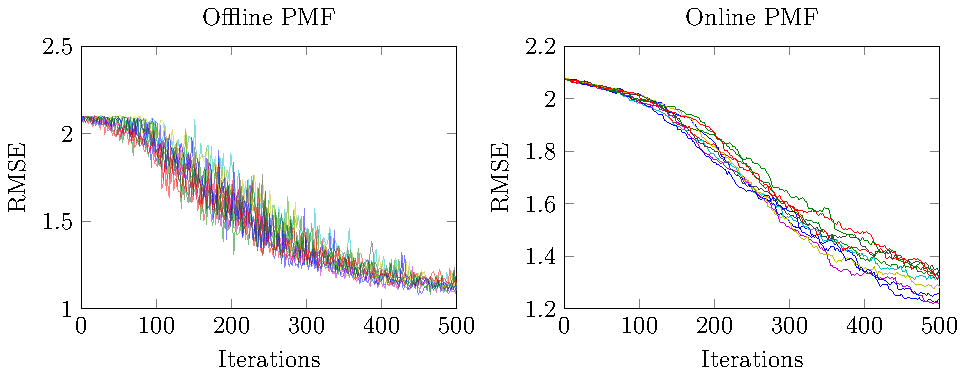
\includegraphics[width=\textwidth]{random_pmf_err}

10 different random sampling simulations on synthetic data.

    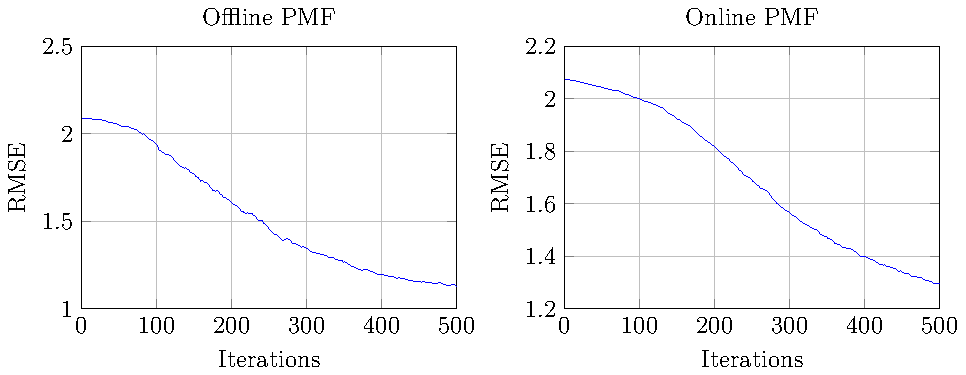
\includegraphics[width=\textwidth]{random_pmf_err_av}
  
Average of 10 simulations.
\end{center}
Original data complete at 1.25\% (with another 1.25\% as validation data)

$\lambda = 0.01$, $D=30$
    \caption{Random Sampling Performance}
    \label{fig:RandomPMF}
\end{figure}


\begin{figure}[!htbp]
  \begin{center}
    \resizebox{\textwidth}{!}{% This file was created by matlab2tikz v0.4.7 running on MATLAB 8.1.
% Copyright (c) 2008--2014, Nico Schlömer <nico.schloemer@gmail.com>
% All rights reserved.
% Minimal pgfplots version: 1.3
% 
% The latest updates can be retrieved from
%   http://www.mathworks.com/matlabcentral/fileexchange/22022-matlab2tikz
% where you can also make suggestions and rate matlab2tikz.
% 
\begin{tikzpicture}

\begin{axis}[%
width=2.20519323671498in,
height=1.97916666666667in,
axis on top,
scale only axis,
xmin=0.5,
xmax=50.5,
y dir=reverse,
ymin=0.5,
ymax=80.5,
name=plot2,
title={Targeted RMSE:1.026}
]
\addplot [forget plot] graphics [xmin=0.5,xmax=50.5,ymin=0.5,ymax=80.5] {eiffel_targeted-1.png};
\end{axis}

\begin{axis}[%
width=2.20519323671498in,
height=1.97916666666667in,
axis on top,
scale only axis,
xmin=0.5,
xmax=50.5,
y dir=reverse,
ymin=0.5,
ymax=80.5,
at=(plot2.left of south west),
anchor=right of south east,
title={Random RMSE:1.150}
]
\addplot [forget plot] graphics [xmin=0.5,xmax=50.5,ymin=0.5,ymax=80.5] {eiffel_targeted-2.png};
\end{axis}

\begin{axis}[%
width=2.20519323671498in,
height=1.97916666666667in,
scale only axis,
xmin=0,
xmax=500,
xlabel={Discovered Samples},
xmajorgrids,
ymin=1,
ymax=2.5,
ylabel={RMSE},
ymajorgrids,
at=(plot2.right of south east),
anchor=left of south west,
title={Target Advantage:1.121},
legend style={draw=black,fill=white,legend cell align=left}
]
\addplot [color=blue,solid]
  table[row sep=crcr]{1	2.31404110645431\\
2	2.31425676410772\\
3	2.31445314839852\\
4	2.31464224670157\\
5	2.3148230859133\\
6	2.31500347878772\\
7	2.31517197314324\\
8	2.31533090214101\\
9	2.31548026212016\\
10	2.31561882833117\\
11	2.31574629352643\\
12	2.31586035565615\\
13	2.31596047556861\\
14	2.31604673729122\\
15	2.31612181590995\\
16	2.31618349045928\\
17	2.31622852518408\\
18	2.31625403286526\\
19	2.31625938910281\\
20	2.31624340397645\\
21	2.31620913357688\\
22	2.31615681412815\\
23	2.31608368123415\\
24	2.31599115706155\\
25	2.31588245005086\\
26	2.31576070749188\\
27	2.3156320303397\\
28	2.31549541257714\\
29	2.31535313799507\\
30	2.31520443325658\\
31	2.31505407474224\\
32	2.31490762190249\\
33	2.31477104322384\\
34	2.31464577823891\\
35	2.31453556266216\\
36	2.31367512137507\\
37	2.31133141183075\\
38	2.30893215992846\\
39	2.30650971262684\\
40	2.30412301276157\\
41	2.30174438542043\\
42	2.29825704023954\\
43	2.29396998338987\\
44	2.28955234333315\\
45	2.28553444213561\\
46	2.28269614348167\\
47	2.27989622368111\\
48	2.27686664953449\\
49	2.27365171102934\\
50	2.27023196965582\\
51	2.26767360984365\\
52	2.26563391361735\\
53	2.26313220664701\\
54	2.26028793925186\\
55	2.25709664736405\\
56	2.25396599323182\\
57	2.25088044068646\\
58	2.24797896815248\\
59	2.24521913427738\\
60	2.24274670183256\\
61	2.23992279056988\\
62	2.23750986731172\\
63	2.23516068852215\\
64	2.23330542066572\\
65	2.23086453116089\\
66	2.2276147279155\\
67	2.22402311282556\\
68	2.21968208736963\\
69	2.21472898482275\\
70	2.21011626628004\\
71	2.20516774286581\\
72	2.20075266788708\\
73	2.1963649015196\\
74	2.19142907996696\\
75	2.18708551114042\\
76	2.18291178800323\\
77	2.17924383977798\\
78	2.17571829649391\\
79	2.1715380888313\\
80	2.16725190729356\\
81	2.16298075377251\\
82	2.15810449879445\\
83	2.15292846205056\\
84	2.14798517609918\\
85	2.14235341644846\\
86	2.13638253886028\\
87	2.12961373481339\\
88	2.1229212739864\\
89	2.11647192798464\\
90	2.11011374985976\\
91	2.10387460599727\\
92	2.09900652328492\\
93	2.09432514790324\\
94	2.08963270718528\\
95	2.08541542179971\\
96	2.08123727813863\\
97	2.07778329008597\\
98	2.07394228885339\\
99	2.06994299047714\\
100	2.06679641801406\\
101	2.06360287140035\\
102	2.06067533630061\\
103	2.05871968567553\\
104	2.05741030392604\\
105	2.05757575632287\\
106	2.05804050046423\\
107	2.05952591243483\\
108	2.06132085158814\\
109	2.06274009832885\\
110	2.0637617846477\\
111	2.06468704623101\\
112	2.06574442631035\\
113	2.06631754050325\\
114	2.06635819082058\\
115	2.06593488729644\\
116	2.06496725444543\\
117	2.06401220274222\\
118	2.0630782332167\\
119	2.06193635207706\\
120	2.06048682458899\\
121	2.05871880217036\\
122	2.0563480204811\\
123	2.05414150344562\\
124	2.05213112336069\\
125	2.04996804171759\\
126	2.04760419035381\\
127	2.04509504656717\\
128	2.04291044538646\\
129	2.04022121803992\\
130	2.0366001720942\\
131	2.03251774271153\\
132	2.02822169638034\\
133	2.02391300233605\\
134	2.02002760422263\\
135	2.01599156130752\\
136	2.01200496345005\\
137	2.00821986163712\\
138	2.00482293919736\\
139	2.00174458210825\\
140	1.99971890284615\\
141	1.99789641480728\\
142	1.9957113768081\\
143	1.99353458222666\\
144	1.99059396165287\\
145	1.98675682851332\\
146	1.98317966584436\\
147	1.9801327821626\\
148	1.97764453794438\\
149	1.9753179673464\\
150	1.97258209449641\\
151	1.9699980130529\\
152	1.96605677583408\\
153	1.96295453677439\\
154	1.96098705423561\\
155	1.95881944915206\\
156	1.95552175575229\\
157	1.9522892400729\\
158	1.947695534894\\
159	1.94338425183434\\
160	1.93944218286694\\
161	1.93696704180037\\
162	1.93398755698765\\
163	1.93069293982857\\
164	1.92656934096279\\
165	1.92218081730403\\
166	1.91706703784556\\
167	1.91277626882804\\
168	1.90787895696652\\
169	1.90220432406231\\
170	1.89624521080799\\
171	1.89238799984753\\
172	1.88754110395697\\
173	1.88328154031879\\
174	1.88015771048206\\
175	1.87741123515482\\
176	1.87496408674419\\
177	1.87348107542113\\
178	1.87191880507184\\
179	1.87017675864246\\
180	1.86636775725631\\
181	1.86310983159721\\
182	1.85947747265745\\
183	1.8555827401434\\
184	1.85105978090019\\
185	1.84631313994686\\
186	1.84005709784503\\
187	1.8332499095589\\
188	1.82598753773178\\
189	1.81881957264238\\
190	1.81224096037214\\
191	1.80618699488285\\
192	1.80033034533977\\
193	1.79532785916755\\
194	1.79060556210099\\
195	1.78732780682547\\
196	1.78556853519003\\
197	1.78405362022411\\
198	1.78297399133508\\
199	1.78148452879606\\
200	1.77996510610784\\
201	1.77829005674299\\
202	1.7764929442072\\
203	1.77429300771002\\
204	1.7714152201878\\
205	1.76868676240815\\
206	1.7668056822737\\
207	1.76522125238592\\
208	1.76455179919605\\
209	1.76420858677775\\
210	1.76455393958375\\
211	1.76523335023632\\
212	1.76538461489872\\
213	1.76597837651021\\
214	1.76620173405808\\
215	1.76546532651268\\
216	1.76396082815346\\
217	1.76214145061607\\
218	1.76026773391705\\
219	1.75743840369648\\
220	1.75287278411311\\
221	1.74860158866225\\
222	1.7422724987361\\
223	1.73462323404525\\
224	1.72694205025914\\
225	1.71843061991188\\
226	1.70951811417603\\
227	1.69986192414951\\
228	1.68962918229449\\
229	1.68057605031386\\
230	1.67150501766814\\
231	1.66400684376912\\
232	1.65655022903279\\
233	1.64960011995681\\
234	1.64397254066184\\
235	1.63795198071727\\
236	1.63219735421561\\
237	1.62577826333049\\
238	1.61870022642254\\
239	1.61104620172168\\
240	1.60377773687994\\
241	1.59726499495644\\
242	1.59081340798708\\
243	1.58294438009457\\
244	1.5748601183041\\
245	1.56700968406842\\
246	1.55898839455494\\
247	1.55013000234112\\
248	1.54206085435789\\
249	1.53472855290209\\
250	1.52785969041305\\
251	1.52064555367461\\
252	1.51460723671974\\
253	1.50922398293897\\
254	1.50395232977853\\
255	1.50077181553249\\
256	1.49974426459448\\
257	1.49934957451923\\
258	1.4986769691068\\
259	1.49678699654613\\
260	1.49533445058535\\
261	1.4940934887377\\
262	1.49336170207339\\
263	1.49236686793284\\
264	1.49130382239467\\
265	1.4893922274161\\
266	1.48793352060723\\
267	1.48495389929656\\
268	1.48314301738427\\
269	1.48014285084888\\
270	1.47775221171514\\
271	1.47476598856971\\
272	1.47187322300268\\
273	1.46856816159847\\
274	1.46529818280839\\
275	1.46111021993423\\
276	1.4576935276672\\
277	1.45436240615844\\
278	1.45096899407841\\
279	1.44459474276816\\
280	1.43784659108841\\
281	1.43092243207188\\
282	1.42426220456286\\
283	1.41814043602794\\
284	1.41218729563923\\
285	1.40651477340576\\
286	1.40045352950293\\
287	1.39548242948141\\
288	1.39286901396478\\
289	1.3910515719995\\
290	1.38924755035503\\
291	1.38737689176505\\
292	1.38590022022086\\
293	1.38458249045794\\
294	1.38328453455804\\
295	1.38254836201366\\
296	1.38108533644439\\
297	1.37954055278099\\
298	1.3776923532805\\
299	1.37575120062471\\
300	1.37377388163956\\
301	1.37093306748052\\
302	1.36766933434279\\
303	1.36329401718814\\
304	1.35849014149051\\
305	1.35478622889932\\
306	1.35049390680744\\
307	1.34586286295709\\
308	1.34163124354616\\
309	1.33766768026547\\
310	1.33386724219489\\
311	1.32943490937536\\
312	1.32614031863094\\
313	1.32249266607618\\
314	1.31798137336285\\
315	1.31377392077356\\
316	1.30955420575781\\
317	1.30506928628429\\
318	1.3001843878094\\
319	1.29474511316326\\
320	1.28934435535143\\
321	1.28198062559397\\
322	1.27462383842209\\
323	1.26716352049109\\
324	1.25887633674218\\
325	1.25112835303693\\
326	1.24336672130161\\
327	1.23454177718307\\
328	1.22622188281774\\
329	1.21778876855187\\
330	1.21106760667605\\
331	1.2054302957322\\
332	1.2002172877545\\
333	1.19623728555625\\
334	1.1924473615307\\
335	1.18859067361414\\
336	1.18607494982103\\
337	1.18430580723422\\
338	1.18366502803976\\
339	1.18314272926967\\
340	1.18173438363381\\
341	1.1819971420057\\
342	1.18233657371344\\
343	1.18186810205928\\
344	1.18169818328992\\
345	1.17908462155883\\
346	1.17597464040899\\
347	1.17300140750746\\
348	1.16937264513645\\
349	1.16622900615379\\
350	1.16271980237193\\
351	1.15831341790407\\
352	1.15453229329104\\
353	1.15118918566305\\
354	1.1500019860983\\
355	1.14870343679925\\
356	1.14678494281984\\
357	1.14608200911847\\
358	1.14524409793541\\
359	1.14302371321857\\
360	1.14157043595355\\
361	1.14015680719264\\
362	1.13808846556812\\
363	1.13653692457014\\
364	1.13544875888625\\
365	1.13499696672541\\
366	1.13446572014099\\
367	1.13405179565849\\
368	1.13412112512648\\
369	1.13452300223401\\
370	1.13480353107401\\
371	1.1338669722912\\
372	1.13294576232921\\
373	1.132210338563\\
374	1.13071617048058\\
375	1.12914031490681\\
376	1.128124706498\\
377	1.12744817632259\\
378	1.12556482665768\\
379	1.12443979316368\\
380	1.12478371786562\\
381	1.12488314142209\\
382	1.12471185282376\\
383	1.12510422313935\\
384	1.12535745156609\\
385	1.12506060368295\\
386	1.12434607261844\\
387	1.12478231671223\\
388	1.12441408052388\\
389	1.12374740746535\\
390	1.12307245067258\\
391	1.12224135194087\\
392	1.1215611240691\\
393	1.1210098422898\\
394	1.12034029137756\\
395	1.11933093895885\\
396	1.11756155263503\\
397	1.11584301135065\\
398	1.11442383961708\\
399	1.11276340231533\\
400	1.11089757263032\\
401	1.10927453118418\\
402	1.10791579506042\\
403	1.10744268242344\\
404	1.10732375320097\\
405	1.1074633022322\\
406	1.10806357081508\\
407	1.10793646890823\\
408	1.10794014435402\\
409	1.10839819512728\\
410	1.10730938175033\\
411	1.10617439324513\\
412	1.10453466388317\\
413	1.10304768922282\\
414	1.10301761356726\\
415	1.10279732761721\\
416	1.10375828039174\\
417	1.10436974558807\\
418	1.10426536456825\\
419	1.10464643864108\\
420	1.1044447879411\\
421	1.10365653993683\\
422	1.10256528887274\\
423	1.09943096337995\\
424	1.09615128131274\\
425	1.09167467091655\\
426	1.08679093852122\\
427	1.08156201467031\\
428	1.07693291616992\\
429	1.07325532038483\\
430	1.0706171877207\\
431	1.06827479097178\\
432	1.06705310232508\\
433	1.0657078321307\\
434	1.06575731746021\\
435	1.06684691277451\\
436	1.06888355298626\\
437	1.07103008848007\\
438	1.07254064176797\\
439	1.07328740480429\\
440	1.07307719095926\\
441	1.07213068209425\\
442	1.07198310934042\\
443	1.07127118163626\\
444	1.06952555473331\\
445	1.06792544667732\\
446	1.0661196179934\\
447	1.06417255961584\\
448	1.06270293503517\\
449	1.06209465557552\\
450	1.06209292254494\\
451	1.06160732920945\\
452	1.06112383559056\\
453	1.06111994158496\\
454	1.06113358993323\\
455	1.06100267653073\\
456	1.06139992254746\\
457	1.06113685194682\\
458	1.06089072855103\\
459	1.06065937068311\\
460	1.06058574796627\\
461	1.06024130901433\\
462	1.06004417084353\\
463	1.05980345998416\\
464	1.05931545814962\\
465	1.05805228352948\\
466	1.05652533583289\\
467	1.05469460630483\\
468	1.05255148442967\\
469	1.04970406114713\\
470	1.04712866146986\\
471	1.04453784588575\\
472	1.04153123897601\\
473	1.039413252842\\
474	1.03765015459116\\
475	1.03641738638663\\
476	1.03532465856552\\
477	1.03374122849738\\
478	1.03258515498343\\
479	1.03134414645722\\
480	1.03024344178858\\
481	1.02961201270084\\
482	1.02847522014646\\
483	1.02696751681409\\
484	1.02520036828126\\
485	1.02337445197715\\
486	1.02168885737384\\
487	1.01919851361261\\
488	1.01650833460998\\
489	1.01382105523529\\
490	1.01112603215788\\
491	1.00840923638358\\
492	1.00590052369843\\
493	1.00589367775222\\
494	1.00761346036835\\
495	1.00919069115692\\
496	1.01159515941495\\
497	1.01459282615493\\
498	1.01999106895151\\
499	1.02786397477042\\
500	1.02605019636602\\
};
\addlegendentry{Random Sampling};

\addplot [color=black!50!green,solid]
  table[row sep=crcr]{1	2.31355651732015\\
2	2.31356566020658\\
3	2.31323047111064\\
4	2.31247525805625\\
5	2.31193696428279\\
6	2.31145193854417\\
7	2.31093760321731\\
8	2.31043973508214\\
9	2.30986109424655\\
10	2.3093435655076\\
11	2.30898671085035\\
12	2.30864489318465\\
13	2.30820843383207\\
14	2.30775296516415\\
15	2.3073548669485\\
16	2.3068288178598\\
17	2.30619055608816\\
18	2.3057069522827\\
19	2.30520927923926\\
20	2.30475000571301\\
21	2.30413569269437\\
22	2.30352414106385\\
23	2.30301512054566\\
24	2.3024955382434\\
25	2.30193859105076\\
26	2.30153708217051\\
27	2.3010051379223\\
28	2.30051534877654\\
29	2.29994291447892\\
30	2.29945023083487\\
31	2.29907116399319\\
32	2.29863697599032\\
33	2.29788191061376\\
34	2.29726981760918\\
35	2.29651062249013\\
36	2.29585655690555\\
37	2.29517344939967\\
38	2.29456680352742\\
39	2.29402472387361\\
40	2.29351516122654\\
41	2.29302829618564\\
42	2.29288682775964\\
43	2.29271841968344\\
44	2.29235791588622\\
45	2.29201660391197\\
46	2.2915751014021\\
47	2.29103424305738\\
48	2.29055564978351\\
49	2.29003343570519\\
50	2.28943130927127\\
51	2.28886570753181\\
52	2.28833922852935\\
53	2.28818564129896\\
54	2.28799540746367\\
55	2.28789202646634\\
56	2.28771875306846\\
57	2.28750145398787\\
58	2.28728428827398\\
59	2.28710510092621\\
60	2.28670656189732\\
61	2.28634603564762\\
62	2.28588314710729\\
63	2.28541111526559\\
64	2.28494262057855\\
65	2.28453364231402\\
66	2.28413089674552\\
67	2.28359477312381\\
68	2.28302093814265\\
69	2.28268708600367\\
70	2.28223511042373\\
71	2.28176184232033\\
72	2.28126717242594\\
73	2.28079297446668\\
74	2.2803656355735\\
75	2.27969874316544\\
76	2.27903953062867\\
77	2.27846202017233\\
78	2.27756814411681\\
79	2.27681290586573\\
80	2.27597403032839\\
81	2.27513707695037\\
82	2.27402024188753\\
83	2.27294902076212\\
84	2.27199835395819\\
85	2.2710276898839\\
86	2.2697347194763\\
87	2.26879429251342\\
88	2.26784079969352\\
89	2.26677967604171\\
90	2.26557021962211\\
91	2.26466243103099\\
92	2.26381607500521\\
93	2.26311471463644\\
94	2.26244964810105\\
95	2.26186807087349\\
96	2.26076155132473\\
97	2.25963258314019\\
98	2.25875329679297\\
99	2.25791141761088\\
100	2.25686573858731\\
101	2.25572592405795\\
102	2.25454928031301\\
103	2.25336322475232\\
104	2.25250255897708\\
105	2.25187232412626\\
106	2.25134479889169\\
107	2.25071510560578\\
108	2.25017918279445\\
109	2.2496880591161\\
110	2.24925324488465\\
111	2.24873767854012\\
112	2.2480038241248\\
113	2.24726301382025\\
114	2.2463969005488\\
115	2.24525240300209\\
116	2.24364835947216\\
117	2.24207123746162\\
118	2.24055931690706\\
119	2.2389567149643\\
120	2.23732229795761\\
121	2.23573699257113\\
122	2.23388171450245\\
123	2.23230185160125\\
124	2.23056109236963\\
125	2.22920217097624\\
126	2.22769863239408\\
127	2.22622243126376\\
128	2.22488642875253\\
129	2.22344695353128\\
130	2.22241580881377\\
131	2.22132801809208\\
132	2.21983992700348\\
133	2.2188245202822\\
134	2.21786568663174\\
135	2.21717745623723\\
136	2.2162851450052\\
137	2.21530871655536\\
138	2.21421916340668\\
139	2.21295558426731\\
140	2.21160435511528\\
141	2.21067295864196\\
142	2.20881540464901\\
143	2.20666734262386\\
144	2.20441060304785\\
145	2.20198414893878\\
146	2.19952582066733\\
147	2.19721614269807\\
148	2.19463938148753\\
149	2.19215652308599\\
150	2.18965317861941\\
151	2.18756822103205\\
152	2.18583830802001\\
153	2.18383660214736\\
154	2.18197198507573\\
155	2.18031696791109\\
156	2.17888854851298\\
157	2.17756213707072\\
158	2.17584279038011\\
159	2.17392945355654\\
160	2.17194265066163\\
161	2.16922434846855\\
162	2.16646160304178\\
163	2.1637116361189\\
164	2.16082364107209\\
165	2.15734057141862\\
166	2.15415698703494\\
167	2.1514066367975\\
168	2.14890651673209\\
169	2.14615350277454\\
170	2.14413273742008\\
171	2.14226017846\\
172	2.13968757996299\\
173	2.13661498013055\\
174	2.13333588295244\\
175	2.1300507050753\\
176	2.12630887857031\\
177	2.12224582471576\\
178	2.11867192574391\\
179	2.11507407032549\\
180	2.11098507086203\\
181	2.10770840563658\\
182	2.104889290405\\
183	2.10235072708847\\
184	2.09951807674364\\
185	2.0972354818042\\
186	2.09493842382219\\
187	2.09235206888047\\
188	2.08900492840267\\
189	2.08606462750574\\
190	2.08312144461488\\
191	2.07977788123497\\
192	2.07594546043688\\
193	2.07211457762552\\
194	2.0681843622986\\
195	2.06414321669297\\
196	2.0604906162847\\
197	2.05753233894327\\
198	2.05423201899248\\
199	2.05069876932702\\
200	2.0473679821959\\
201	2.04481918340028\\
202	2.04213791189998\\
203	2.0390743216435\\
204	2.03626366356825\\
205	2.03344259229105\\
206	2.0296496053707\\
207	2.02654219782157\\
208	2.02333550605557\\
209	2.01963165431823\\
210	2.01598638265753\\
211	2.01245431170046\\
212	2.0095302379501\\
213	2.00627564993958\\
214	2.00267460524632\\
215	1.99927350947372\\
216	1.99545176179751\\
217	1.99212371143856\\
218	1.98913316041108\\
219	1.98537883499722\\
220	1.98155635848432\\
221	1.97741610291749\\
222	1.97382064045637\\
223	1.97017401900578\\
224	1.96711881540769\\
225	1.96430821015927\\
226	1.96141564832038\\
227	1.958557223124\\
228	1.95586161344697\\
229	1.95321428321351\\
230	1.95005995767043\\
231	1.94599291440712\\
232	1.94224746827753\\
233	1.93889185079\\
234	1.9349160046348\\
235	1.93013694909405\\
236	1.92471823088953\\
237	1.91993477586086\\
238	1.91466202965007\\
239	1.90985163871627\\
240	1.90455524692571\\
241	1.89900895505723\\
242	1.89326806440131\\
243	1.88814590029984\\
244	1.88326580482791\\
245	1.87883905898706\\
246	1.87425890519452\\
247	1.87025848495357\\
248	1.86614586161227\\
249	1.86331840911406\\
250	1.86071537435874\\
251	1.85796650288101\\
252	1.8547408156344\\
253	1.85080737366106\\
254	1.84665078127658\\
255	1.84256870039945\\
256	1.83861585051675\\
257	1.83465159601838\\
258	1.82973671167983\\
259	1.82400045341437\\
260	1.81822594015466\\
261	1.81227032416754\\
262	1.80743203667508\\
263	1.80275653585674\\
264	1.79683008994035\\
265	1.79063059871071\\
266	1.78427029327884\\
267	1.77833648132276\\
268	1.77361240352778\\
269	1.76842008591514\\
270	1.76389218607563\\
271	1.75886923726544\\
272	1.75405254603892\\
273	1.75066941134979\\
274	1.7477370775049\\
275	1.74453956434007\\
276	1.74127279251289\\
277	1.73738817239367\\
278	1.73415377285533\\
279	1.73099936742665\\
280	1.72738630448789\\
281	1.72360531961805\\
282	1.71896026865338\\
283	1.71411201511617\\
284	1.70979863797483\\
285	1.70519048249347\\
286	1.70087936184304\\
287	1.69590395804856\\
288	1.6911186405967\\
289	1.68697888833162\\
290	1.68214326790307\\
291	1.67743869335299\\
292	1.67083854877209\\
293	1.66462757707148\\
294	1.65866560560533\\
295	1.65227835438196\\
296	1.64715820248178\\
297	1.64152075278102\\
298	1.63621000524499\\
299	1.62965407947917\\
300	1.62371612644748\\
301	1.61951417326594\\
302	1.61332497433663\\
303	1.60883886710821\\
304	1.60478796805914\\
305	1.59966460807922\\
306	1.5940661309777\\
307	1.58860722800978\\
308	1.58481146956848\\
309	1.58095711321011\\
310	1.57677553295084\\
311	1.57441617524935\\
312	1.57056676613693\\
313	1.56688659176\\
314	1.56392603430254\\
315	1.561750734419\\
316	1.55820990489985\\
317	1.55576847191101\\
318	1.55360732752056\\
319	1.55154203165938\\
320	1.54884192548582\\
321	1.54646641493389\\
322	1.54366942364416\\
323	1.54046459151378\\
324	1.53697110487591\\
325	1.5354765525073\\
326	1.53361153397819\\
327	1.5314066375921\\
328	1.52963474571191\\
329	1.52648326253657\\
330	1.52298013008416\\
331	1.51795679651879\\
332	1.51310225213702\\
333	1.50871799102033\\
334	1.50376595715692\\
335	1.49873932647599\\
336	1.49280938967234\\
337	1.4863361877881\\
338	1.48166767130697\\
339	1.47736447537105\\
340	1.47387018589748\\
341	1.47054689114904\\
342	1.46610408819733\\
343	1.46081470600565\\
344	1.45486404158116\\
345	1.45026723130047\\
346	1.44610228283337\\
347	1.44152533000746\\
348	1.43619611716834\\
349	1.4311557371892\\
350	1.42562613008549\\
351	1.4207122329411\\
352	1.41650240542642\\
353	1.41305398323408\\
354	1.40915033939929\\
355	1.40540508037387\\
356	1.40150969069792\\
357	1.39800144746147\\
358	1.39475162841027\\
359	1.3919500355791\\
360	1.38914433808517\\
361	1.386423698983\\
362	1.38284605066004\\
363	1.37941175521707\\
364	1.37575801931725\\
365	1.37320810514657\\
366	1.37112538095449\\
367	1.36783687539288\\
368	1.36441412118992\\
369	1.36113338263728\\
370	1.3579560438647\\
371	1.35468091401008\\
372	1.35020457016068\\
373	1.34611497351895\\
374	1.34111855903329\\
375	1.33516199651132\\
376	1.33145801863336\\
377	1.32818208120271\\
378	1.32567420348368\\
379	1.32217228766702\\
380	1.31964647284392\\
381	1.31816388305518\\
382	1.31583119173864\\
383	1.31351763448467\\
384	1.31202299607488\\
385	1.31056639349238\\
386	1.30826900045043\\
387	1.30523035684101\\
388	1.30288138884817\\
389	1.30093762171791\\
390	1.29919037542968\\
391	1.29811075128451\\
392	1.2974738594748\\
393	1.29711022871794\\
394	1.2964452310665\\
395	1.29533623856166\\
396	1.2946520691074\\
397	1.29424866093843\\
398	1.29351565681501\\
399	1.29217918793326\\
400	1.29083999199595\\
401	1.28925463990045\\
402	1.28794199039559\\
403	1.28593205195636\\
404	1.28466638407692\\
405	1.28312433490653\\
406	1.28103104161751\\
407	1.27903128629618\\
408	1.27802180788597\\
409	1.27770980550536\\
410	1.27784576679104\\
411	1.27741453962001\\
412	1.27742121002841\\
413	1.27780035373636\\
414	1.27794515392025\\
415	1.27803689352109\\
416	1.27819249138332\\
417	1.27737542603794\\
418	1.2759607006949\\
419	1.2738828867809\\
420	1.27140033592091\\
421	1.26685396905252\\
422	1.26228056154393\\
423	1.2576233407123\\
424	1.25288458626841\\
425	1.24709661094785\\
426	1.24202231376621\\
427	1.2367316677216\\
428	1.23367805614844\\
429	1.23143821712816\\
430	1.23132470414198\\
431	1.23115382844202\\
432	1.23100088575675\\
433	1.2314537007536\\
434	1.23229911512576\\
435	1.23293909744274\\
436	1.23367727907891\\
437	1.23307984357647\\
438	1.23206684418599\\
439	1.2309110534019\\
440	1.22987252513006\\
441	1.22913957989914\\
442	1.22887892265067\\
443	1.22829587705842\\
444	1.22757450227168\\
445	1.22597517797487\\
446	1.22400538888464\\
447	1.22388583392221\\
448	1.22373458451004\\
449	1.2233521087221\\
450	1.22263785526085\\
451	1.22131852412864\\
452	1.22062026386659\\
453	1.22021292428176\\
454	1.22033195199516\\
455	1.22052368021259\\
456	1.21910421187171\\
457	1.21675382408037\\
458	1.21413943195238\\
459	1.21161529390472\\
460	1.20913328073211\\
461	1.20583117941093\\
462	1.20261026283376\\
463	1.19988553048394\\
464	1.19728789330464\\
465	1.19408323906272\\
466	1.19312738840717\\
467	1.19190374852315\\
468	1.19167086161593\\
469	1.19119287651117\\
470	1.19092384476178\\
471	1.19046602519544\\
472	1.18993201988666\\
473	1.18934112757251\\
474	1.18934462673543\\
475	1.18894310518462\\
476	1.1886832344409\\
477	1.18760710819821\\
478	1.18659014254121\\
479	1.18648505220062\\
480	1.18636317524915\\
481	1.18638130170429\\
482	1.18633115092021\\
483	1.18564678128192\\
484	1.18381768014321\\
485	1.18231248589041\\
486	1.18085508989434\\
487	1.17852263282527\\
488	1.17582717816612\\
489	1.1722988935254\\
490	1.17012608816856\\
491	1.16824489926652\\
492	1.16577577368752\\
493	1.16353777731863\\
494	1.16130843133576\\
495	1.15904659832518\\
496	1.15760989371068\\
497	1.15788520543675\\
498	1.15415533619797\\
499	1.15273699895913\\
500	1.1501807272355\\
};
\addlegendentry{Targeted};

\end{axis}
\end{tikzpicture}%}
\end{center}
Original data complete at 1.25\% (with another 1.25\% as validation data)

Data is downsampled and rounded Eiffel tower image to fit $[1,5]$.

Online PMF, $\lambda = 0.01$, $D=30$
    \caption{Minimum Knowledge Search on Eiffel Tower}
    \label{fig:eiffel_active_mks}
\end{figure}

\begin{figure}[!htbp]
  \begin{center}
  \resizebox{\textwidth}{!}{% This file was created by matlab2tikz v0.4.7 running on MATLAB 8.1.
% Copyright (c) 2008--2014, Nico Schlömer <nico.schloemer@gmail.com>
% All rights reserved.
% Minimal pgfplots version: 1.3
% 
% The latest updates can be retrieved from
%   http://www.mathworks.com/matlabcentral/fileexchange/22022-matlab2tikz
% where you can also make suggestions and rate matlab2tikz.
% 
\begin{tikzpicture}

\begin{axis}[%
width=2.22901570048309in,
height=2.67421875in,
scale only axis,
xmin=0,
xmax=500,
xlabel={Discovered Samples},
xmajorgrids,
ymin=1,
ymax=2.4,
ylabel={RMSE},
ymajorgrids,
name=plot2,
title={Target Advantage:1.036}
]
\addplot [color=blue,solid,forget plot]
  table[row sep=crcr]{1	2.08955683240127\\
4	2.08120851852688\\
7	2.07534150943872\\
10	2.07113303496436\\
13	2.06449693474286\\
16	2.05704264681726\\
19	2.05270905397449\\
22	2.04703296014939\\
25	2.04208407964867\\
28	2.04378475917784\\
31	2.04058668635071\\
34	2.03556993833398\\
37	2.03064629409764\\
40	2.02436925212641\\
43	2.01630214197685\\
46	2.00858306459747\\
49	2.00474788950457\\
52	1.99800714102804\\
55	1.99003168036556\\
58	1.98764933705001\\
61	1.98809106918327\\
64	1.98630261502406\\
67	1.99195388990038\\
70	1.98620506412944\\
73	1.98445532070391\\
76	1.98382450546172\\
79	1.98455966024057\\
82	1.97646683456422\\
85	1.96064124215243\\
88	1.95283686987202\\
91	1.93738612400345\\
94	1.93214600524994\\
97	1.91391960242186\\
100	1.91008773200848\\
103	1.89804432538063\\
106	1.88349742225093\\
109	1.86923963085806\\
112	1.85975494582399\\
115	1.84732426623339\\
118	1.8398495885267\\
121	1.832029971429\\
124	1.83430118916913\\
127	1.80795489907222\\
130	1.77619551220851\\
133	1.75970980909346\\
136	1.7363092025138\\
139	1.7308471324561\\
142	1.7189590414173\\
145	1.71191578824767\\
148	1.70437376954023\\
151	1.70916406262316\\
154	1.68804972090553\\
157	1.67252104282444\\
160	1.6456634847308\\
163	1.6189741819892\\
166	1.60464948168617\\
169	1.60621676416582\\
172	1.57284008241142\\
175	1.55963179728716\\
178	1.56046771701689\\
181	1.54846115155033\\
184	1.53460295704343\\
187	1.50195343564028\\
190	1.51350246604894\\
193	1.50136850325632\\
196	1.500017435562\\
199	1.48872959731716\\
202	1.45955281676692\\
205	1.45183610033175\\
208	1.44470401288984\\
211	1.43038999419091\\
214	1.41621633424817\\
217	1.40895193528978\\
220	1.40490722731198\\
223	1.396597683391\\
226	1.37752238107544\\
229	1.37177035643585\\
232	1.3698549459506\\
235	1.36553827006921\\
238	1.35426931375028\\
241	1.34750221013096\\
244	1.34244396515889\\
247	1.34136835659876\\
250	1.32563093220512\\
253	1.32325186841771\\
256	1.31697368837166\\
259	1.31529664088897\\
262	1.30886539752246\\
265	1.30108529262825\\
268	1.29502695609685\\
271	1.29228516232994\\
274	1.28792343170974\\
277	1.27880846069708\\
280	1.26935057885263\\
283	1.26864585571813\\
286	1.26427846155713\\
289	1.2591742299134\\
292	1.26431376521135\\
295	1.26994369095501\\
298	1.27092981547445\\
301	1.26880710014083\\
304	1.26349607498073\\
307	1.25935107064976\\
310	1.2548235719608\\
313	1.25282164688069\\
316	1.24925235677718\\
319	1.24874124430829\\
322	1.25197381221379\\
325	1.25266164126656\\
328	1.24966641544741\\
331	1.2443374114334\\
334	1.24173225322926\\
337	1.23843352871422\\
340	1.23818825005499\\
343	1.23902379365268\\
346	1.23499772792284\\
349	1.23310897961122\\
352	1.23218725326399\\
355	1.23832991175924\\
358	1.238352173016\\
361	1.23102789884616\\
364	1.23171407062859\\
367	1.23140279669778\\
370	1.23099437531552\\
373	1.2311049103155\\
376	1.22607044586302\\
379	1.21978483012963\\
382	1.22116626892908\\
385	1.21695925522813\\
388	1.21708073601571\\
391	1.21110506887662\\
394	1.20724445965935\\
397	1.20642265008572\\
400	1.20622462881926\\
403	1.20412882474165\\
406	1.20083061242515\\
409	1.19837280792117\\
412	1.20172505403672\\
415	1.20319101683298\\
418	1.20191803799231\\
421	1.19830110356644\\
424	1.20109288641826\\
427	1.20291675388244\\
430	1.20261455828073\\
433	1.19846430481434\\
436	1.19890943711771\\
439	1.19618381857365\\
442	1.1904762367084\\
445	1.18813768343454\\
448	1.18471312579485\\
451	1.1864199656993\\
454	1.18810129570592\\
457	1.18920911889499\\
460	1.18916307499863\\
463	1.18851670119718\\
466	1.18460260788554\\
469	1.17787772718249\\
472	1.16776406720888\\
475	1.16028534380028\\
478	1.15724755862622\\
481	1.15250980635763\\
484	1.14852187450615\\
487	1.14589696645781\\
490	1.14618821808225\\
493	1.14132401541564\\
496	1.13114833734571\\
499	1.13285082354089\\
500	1.08992714273505\\
};
\addplot [color=black!50!green,solid,forget plot]
  table[row sep=crcr]{1	2.08737177550677\\
4	2.08467184403021\\
7	2.08298650087891\\
10	2.08348084945761\\
13	2.08235832565932\\
16	2.08278336567022\\
19	2.07997182596675\\
22	2.07911563225928\\
25	2.07822621974444\\
28	2.07619799809029\\
31	2.07509690461574\\
34	2.07037368540558\\
37	2.06796467565784\\
40	2.06249287777274\\
43	2.06005976089149\\
46	2.05720714465723\\
49	2.0496930022108\\
52	2.04530723149985\\
55	2.03888774106181\\
58	2.03873361093176\\
61	2.03199201729195\\
64	2.02591876819778\\
67	2.01848311414454\\
70	2.01262361605077\\
73	2.00395155190626\\
76	1.99462540594667\\
79	1.9852882756053\\
82	1.98091641778124\\
85	1.97347796749868\\
88	1.96446618648546\\
91	1.95785514086079\\
94	1.95138422004017\\
97	1.94229146720604\\
100	1.93366901648982\\
103	1.92342241018382\\
106	1.92051777604366\\
109	1.91496899516326\\
112	1.90839163752708\\
115	1.89586488086919\\
118	1.88066140255096\\
121	1.87395392292007\\
124	1.87550781674251\\
127	1.87264828173258\\
130	1.85683936289269\\
133	1.83307619089402\\
136	1.81464118524864\\
139	1.82249171408737\\
142	1.81510203517035\\
145	1.81115487870425\\
148	1.78991566680894\\
151	1.78768268232496\\
154	1.77419933459181\\
157	1.75914470656101\\
160	1.74201480568861\\
163	1.73337351081135\\
166	1.73037832871174\\
169	1.72524028710671\\
172	1.7172640519419\\
175	1.70530684126998\\
178	1.69022289382998\\
181	1.67781688837803\\
184	1.6651866018857\\
187	1.65786833325152\\
190	1.64163461056598\\
193	1.64621427296132\\
196	1.6386410457844\\
199	1.64045407738492\\
202	1.61837347420205\\
205	1.60981307131975\\
208	1.59221952958318\\
211	1.58892920883708\\
214	1.58329322993786\\
217	1.58301614026078\\
220	1.567965103681\\
223	1.55038370751194\\
226	1.53919574761702\\
229	1.53327736766467\\
232	1.52476495571093\\
235	1.50581086034833\\
238	1.49171998420279\\
241	1.49342951724959\\
244	1.5007717380585\\
247	1.50204426605883\\
250	1.49192696470451\\
253	1.48121566474336\\
256	1.46672052014451\\
259	1.45844805265428\\
262	1.44355779059618\\
265	1.43703738035327\\
268	1.4253302052287\\
271	1.42074401790011\\
274	1.41449212897748\\
277	1.40253724549153\\
280	1.40069222665835\\
283	1.39180532175089\\
286	1.38940725648008\\
289	1.38487970543042\\
292	1.38110597813458\\
295	1.3745230010058\\
298	1.36230351141792\\
301	1.3501871378517\\
304	1.3412095644929\\
307	1.33173351861769\\
310	1.32304550636488\\
313	1.31840292381511\\
316	1.31334104190201\\
319	1.31933152266431\\
322	1.31495091989763\\
325	1.31047964925082\\
328	1.29756420173432\\
331	1.29097480308478\\
334	1.28685145817632\\
337	1.27805122623317\\
340	1.27212012515377\\
343	1.26156765537743\\
346	1.2546533090913\\
349	1.2459105816125\\
352	1.24972460480505\\
355	1.24957136202949\\
358	1.25251678013392\\
361	1.25017249793226\\
364	1.24889540351554\\
367	1.24207233711686\\
370	1.23558814397032\\
373	1.22809686061264\\
376	1.23060254216309\\
379	1.22558605980194\\
382	1.22682227549603\\
385	1.21920191679697\\
388	1.21968643397675\\
391	1.21442053358153\\
394	1.21472677378805\\
397	1.2076025372052\\
400	1.20488826736279\\
403	1.20264160565174\\
406	1.19732675748935\\
409	1.19427745019973\\
412	1.18787560986912\\
415	1.18824687142166\\
418	1.18569285163679\\
421	1.18301310411735\\
424	1.17815756614337\\
427	1.1733234895432\\
430	1.170920066358\\
433	1.16705564895868\\
436	1.16758311592514\\
439	1.16291304863818\\
442	1.15974434515618\\
445	1.15677495393665\\
448	1.15445458443966\\
451	1.15467135208282\\
454	1.15233728237269\\
457	1.15149389611694\\
460	1.1479855493612\\
463	1.14753512073225\\
466	1.14791346977819\\
469	1.14654344230593\\
472	1.14456063957849\\
475	1.13791032233366\\
478	1.13570570496753\\
481	1.13306893975319\\
484	1.13318773014601\\
487	1.13032176593801\\
490	1.12855069123371\\
493	1.12682279115302\\
496	1.12434455628116\\
499	1.11658124448945\\
500	1.10494857330348\\
};
\end{axis}

\begin{axis}[%
width=2.22901570048309in,
height=2.67421875in,
axis on top,
scale only axis,
xmin=0.5,
xmax=50.5,
y dir=reverse,
ymin=0.5,
ymax=80.5,
at=(plot2.left of south west),
anchor=right of south east,
title={Targeted RMSE:1.090}
]
\addplot [forget plot] graphics [xmin=0.5,xmax=50.5,ymin=0.5,ymax=80.5] {cks_end_synth-1.png};
\end{axis}

\begin{axis}[%
width=2.22901570048309in,
height=2.67421875in,
axis on top,
scale only axis,
xmin=0.5,
xmax=50.5,
y dir=reverse,
ymin=0.5,
ymax=80.5,
at=(plot2.right of south east),
anchor=left of south west,
title={Targeted Samples}
]
\addplot [forget plot] graphics [xmin=0.5,xmax=50.5,ymin=0.5,ymax=80.5] {cks_end_synth-2.png};
\end{axis}
\end{tikzpicture}%}
Average of 10 simulations.
\end{center}
Original data complete at 1.25\% (with another 1.25\% as validation data)

Note how the performance at the beginning is very good but as soon as information about most clusters is gained performance is worse due to an area of little information in a cluster of high information being ignored.

$\lambda = 0.01$, $D=7$
    \caption{CKS Performance on Synthetic Data - Local Cluster Oversight}
    \label{fig:cks_end_synth}
\end{figure}

\section{Code}

This contains samples of the main code used throughout the project. The full code can be found on \url{https://github.com/sg3510/al_proj/}
\subsection{PMF}
A version with validation set and overfitting is present on github.
\lstinputlisting[label=pmfcode,caption=PMF Gradient Descent]{Code/matrixfactoriser/pmf_func.m}

\subsection{CKS}
\lstinputlisting[label=ckscode,caption=Clustered Knowledge Selection criteria generation]{Code/routines/CKS_UV_cluster.m}

\subsection{Matrix-Normal Variance calculation}

\lstinputlisting[label=mnvarcode,caption=Minimum Variance Calculation]{Code/routines/MN_V.m}

\lstinputlisting[label=e2calc,caption=2 Input sample expectation based on parameters]{Code/routines/expect_norm2.m}

\lstinputlisting[label=e4calc,caption=4 Input sample expectation based on parameters]{Code/routines/expect_norm2.m}


\subsection{Main Runtime Code for active sampling simulation}
\lstinputlisting[label=maincalc,caption=Code base for Active Sampling]{Code/main.m}
% ------------------------------------------------------------------------

%%% Local Variables: 
%%% mode: latex
%%% TeX-master: "../thesis"
%%% End: 

\end{document}
